% Hint: "include" did not work for me using:
% This is pdfTeX, Version 3.1415926-2.4-1.40.13 (TeX Live 2012/Debian)
% Replaced "include" with "input" to make it work.

% $Id: header.tex 1229 2009-10-23 13:58:42Z inf6254 $
%%%%%%%%%%%%%%%%%%%%%%%%%%%%%%%%%%%%%%%%%%%%%%%%%%%%%%%%%%%%%%%%%%%%%%%
\documentclass
  [ %twoside            % beidseitiger Druck
  , openright           % Kapitel beginnen auf einer rechten Seite
  , listof=totoc        % Verzeichnisse im Inhaltsverzeichnis
  , bibliography=totoc  % Literaturverzeichnis im Inhaltsverzeichnis
  , parskip=half        % Absätze durch einen vergrößerten Zeilenabstand getrennt
%  , draft              % Entwurfsversion
  ]{scrreprt}           % Dokumentenklasse: KOMA-Script Buch

\bibliographystyle{alpha}


%%%%%%%%%%%%%%%%%%%%%%%%%%%%%%%%%%%%%%%%%%%%%%%%%%%%%%%%%%%%%%%%%%%%%%%
% Packages
%%%%%%%%%%%%%%%%%%%%%%%%%%%%%%%%%%%%%%%%%%%%%%%%%%%%%%%%%%%%%%%%%%%%%%%
\usepackage{scrhack}

 
\usepackage{ifpdf}
\ifpdf
  \usepackage{ae}               % Fonts für pdfLaTeX, falls keine cm-super-Fonts installiert
  \usepackage{microtype}        % optischer Randausgleich, falls pdflatex verwandt
  \usepackage[pdftex]{graphicx} % Grafiken in pdfLaTeX
\else
  \usepackage[dvips]{graphicx}  % Grafiken und normales LaTeX
\fi

\usepackage[a4paper,
            inner=2.0cm,outer=2.0cm,bindingoffset=0.5cm,
            top=1.5cm,bottom=1.5cm,
            footskip=1.0cm,includeheadfoot]{geometry}
            
\usepackage[utf8]{inputenc}         % Input encoding (allow direct use of special characters like "ä")
%\usepackage[english]{babel}
\usepackage[ngerman]{babel}
\usepackage[T1]{fontenc}
\usepackage[automark]{scrlayer-scrpage} % Schickerer Satzspiegel mit KOMA-Script
\usepackage{setspace}           	    % Allow the modification of the space between lines
\usepackage{booktabs}           	    % Netteres Tabellenlayout
\usepackage{multicol}                   % Mehrspaltige Bereiche
\usepackage{quotchap}                   % Beautiful chapter decoration
\usepackage{acronym}                    % list of acronyms and abbreviations
\usepackage{subfig}                     % allow sub figures
\usepackage{tabularx}                   % Tabellen mit fester Breite
\usepackage{lipsum}                     % für Blindtexte
\usepackage{titlesec}                   % für eigene Überschriftenstile
\usepackage{nameref}                    % Namen von refs bekommen (Kapitel etc.)
\usepackage{todonotes}                  % ToDo-Kommentare und Auflistung
\usepackage{float}                      % Bilder positionieren
\usepackage{interval}                   % Intervalle
\usepackage{amssymb}                    % Mathekrams, z.B. \mathbb für Mengen
\usepackage{amsmath}                    % Noch mehr Mathekrams, für argmax etc.
\usepackage[ruled,vlined]{algorithm2e}  % Pseudocode, Algorithmenbeschreibung
\usepackage{listings}                   % Nice listings with frames etc.
\usepackage{lstautogobble}              % Auto gobbling for listings.
\usepackage{stackengine}                % Stacking of objects
 


%%%%%%%%%%%%%%%%%%%%%%%%%%%%%%%%%%%%%%%%%%%%%%%%%%%%%%%%%%%%%%%%%%%%%%%
% User Commands
%%%%%%%%%%%%%%%%%%%%%%%%%%%%%%%%%%%%%%%%%%%%%%%%%%%%%%%%%%%%%%%%%%%%%%%

\newcommand*{\Name}[1]{\textsc{#1}}
\newcommand*{\Befehl}[1]{\texttt{#1}}
\newcommand*{\Fachbegriff}[1]{\emph{#1}}
\newcommand*{\FachbegriffMitAbk}[2]{\emph{#1} (#2)}
\newcommand*{\ErsterFachbegriffMitAbk}[3]{\emph{#1} (#2)\acused{#3}}
\newcommand*{\sogenannt}[1]{\glqq{}#1\grqq{}}
\newcommand*{\aufzaehlung}[1]{\glqq{}#1\grqq{}}
\newcommand{\hiddensection}[1]{ \stepcounter{section} \section*{#1}}
\newcommand*{\inlinecode}[1]{\texttt{#1}}
\newcommand*{\filepath}[1]{\texttt{#1}}


\DeclareMathOperator*{\mathmax}{max}
\DeclareMathOperator*{\mathmin}{min}
\DeclareMathOperator*{\argmax}{arg\,max}
\DeclareMathOperator*{\argmin}{arg\,min}


%%%%%%%%%%%%%%%%%%%%%%%%%%%%%%%%%%%%%%%%%%%%%%%%%%%%%%%%%%%%%%%%%%%%%%%
% Layout
%%%%%%%%%%%%%%%%%%%%%%%%%%%%%%%%%%%%%%%%%%%%%%%%%%%%%%%%%%%%%%%%%%%%%%%

\lstset{ % For custom listings
    numbers=left, 
    numberstyle=\small, 
    numbersep=15pt, 
    frame = single, 
    language=Java, 
    framexleftmargin=25pt,
    autogobble=true
}

\pagestyle{scrheadings}
% \pagestyle{empty}
\clubpenalty = 10000
\widowpenalty = 10000
\displaywidowpenalty = 10000

\makeatletter
\renewcommand{\fps@figure}{htbp}
\makeatother


%% Document properties %%%%%%%%%%%%%%%%%%%%%%%%%%%%%%%%%%%%%%%%%%%%%%%%
\newcommand{\projname}{Reinforcement-Utility-Village}

% Der Titel ist Banane, hier soll einfach irgendwas stehen
\newcommand{\titel}{Anwendung von Reinforcement Learning zur Entwicklung authentischer Spielwelten mithilfe bedürfnisbasierter Agenten}
\newcommand{\authorname}{Tobias Jansing}
\newcommand{\thesisname}{Master Thesis}
\newcommand{\untertitel}{Ein alternativer Ansatz zur Entwicklung von \textit{Non-Player-Characters} anhand einer Dorfsimulation mit Unity}
\newcommand{\Datum}{26 Februar 2020}

\ifpdf
  \usepackage{hyperref}
  \definecolor{darkblue}{rgb}{0,0,.5}
  \hypersetup
  	{ colorlinks=true
  	, breaklinks=true
    , linkcolor=darkblue
    , menucolor=darkblue
    , urlcolor=darkblue
    , citecolor=darkblue
    , pdftitle={\projname -- \untertitel}
    , pdfsubject={\thesisname}
    , pdfauthor={\authorname}
    }
\else
\fi

%% Listings %%%%%%%%%%%%%%%%%%%%%%%%%%%%%%%%%%%%%%%%%%%%%%%%%%%%%%%%%
\usepackage{listings}
\KOMAoptions{listof=totoc} % necessary because of scrhack
\renewcommand{\lstlistlistingname}{List of Listings}
\lstset
  { basicstyle=\small\ttfamily
  , breaklines=true
  , captionpos=b
  , showstringspaces=false
  , keywordstyle={}
  }

\lstnewenvironment{inlinehaskell}
{\spacing{1}\lstset{language=haskell,nolol,aboveskip=\bigskipamount}}
{\endspacing}

\lstnewenvironment{inlinexml}
{\spacing{1}\lstset{language=XML,nolol,aboveskip=\bigskipamount}}
{\endspacing}

\newcommand{\haskellinput}[2][]{
  \begin{spacing}{1}
  \lstinputlisting[language=Haskell,nolol,aboveskip=\bigskipamount,#1]{#2}
  \end{spacing}
}

\newcommand{\haskellcode}[2][]{\mylisting[#1,language=Haskell]{#2}}

\newcommand{\mylisting}[2][]{
\begin{spacing}{1}
\lstinputlisting[frame=lines,aboveskip=2\bigskipamount,#1]{#2}
\end{spacing}
}


\begin{document}




%%%%%%%%%%%%%%%%%%%%%%%%%%%%%%%%%%%%%%%%%%%%%%%%%%%%%%%%%%%%%%%%%%%
%%%%%%%%%%%%%%%%%%%%%%%%% ! TITLE STYLES ! %%%%%%%%%%%%%%%%%%%%%%%%
%%%%%%%%%%%%%%%%%%%%%%%%%%%%%%%%%%%%%%%%%%%%%%%%%%%%%%%%%%%%%%%%%%%
% Chapter numbering depth. This does not change the structure of the chapter listing!
\setcounter{secnumdepth}{3} 

\titleformat{\section}
{\normalfont\Large\bfseries}{\thesection}{1em}{}
\titleformat{\subsection}
{\normalfont\large\bfseries}{\thesubsection}{1em}{}
\titleformat{\subsubsection}
{\normalfont\normalsize\bfseries}{\thesubsubsection}{1em}{}
\titleformat{\paragraph}[runin]
{\normalfont\normalsize\bfseries}{\theparagraph}{1em}{}
\titleformat{\subparagraph}[runin]
{\normalfont\normalsize\bfseries}{\thesubparagraph}{1em}{}

%%%%%%%%%%%%%%%%%%%%%%%%%%%%%%%%%%%%%%%%%%%%%%%%%%%%%%%%%%%%%%%%%%%
%%%%%%%%%%%%%%%%%%%%%%%%%%%% ! TODOS ! %%%%%%%%%%%%%%%%%%%%%%%%%%%%
%%%%%%%%%%%%%%%%%%%%%%%%%%%%%%%%%%%%%%%%%%%%%%%%%%%%%%%%%%%%%%%%%%%
% \listoftodos

%%%%%%%%%%%%%%%%%%%%%%%%%%%%%%%%%%%%%%%%%%%%%%%%%%%%%%%%%%%%%%%%%%%
%%%%%%%%%%%%%%%%%%%%%%%%%%%% ! START ! %%%%%%%%%%%%%%%%%%%%%%%%%%%%
%%%%%%%%%%%%%%%%%%%%%%%%%%%%%%%%%%%%%%%%%%%%%%%%%%%%%%%%%%%%%%%%%%%
\titlehead{
  \centering
  
\includegraphics[width=.5\textwidth]{images/fhw}\\
  \bigskip
  \textsc{\Large Department of Computer Science}
}

\subject{\thesisname}
\title{\titel}
\subtitle{\Large \untertitel}
\date{\vspace{-1cm}{\small Eingereicht am:}\\\medskip\Datum}
\author{}
\publishers{\vfill
  \normalsize
  \begin{minipage}{13cm}
  
    \raggedright
    {\small Eingereicht von:} \\
    \smallskip
  	{\Large \authorname}\\
     Billwerder Neuer Deich 6\\
     20539 Hamburg\\
     Tel.: (+49\,157)~52\,56\,65\,78\\
     E-mail: tob.jansing@gmail.com\\

    
    \bigskip
    \bigskip
       
    \begin{multicols}{2}
      \raggedright{\small Referent:}\\
      \smallskip{\large Prof. Dr. Ulrich Hoffmann}\\
      Fachhochschule Wedel\\
      Feldstraße 143\\
      22880 Wedel\\
      Phone: (041\,03)~80\,48-41\\
      E-mail: uh@fh-wedel.de\\


      \raggedleft{\small Koreferent:}\\
      \smallskip{\large Prof. Dr. Michael Predeschly}\\
      Fachhochschule Wedel\\
      Feldstraße 143\\
      22880 Wedel\\
      Phone: (041\,03)~80\,48-45\\
      E-mail: mpr@fh-wedel.de\\
    \end{multicols}
 \end{minipage}
}

\uppertitleback{
  {\huge \titel}\bigskip\\  
  {\Large \untertitel}\bigskip\\
  {\large \thesisname von \authorname}
  % \begin{abstract}
  % Das ist ein Einleitungstext!
  % \end{abstract}
}

% \lowertitleback{
    % warum wird das nicht angezeigt?!?
    % Copyright {\small \copyright} 2020 \authorname \bigskip\\
    % IRGENDEIN COYPRIGHT TEXT MUSS DER HIER SEIN?
    % Layout done with {\rmfamily \LaTeXe}, {\sffamily \KOMAScript} and {\rmfamily % B\textsc{ib}\TeX}.
% }

\maketitle



\pagenumbering{roman}
\hiddensection{Kurzfassung}
Die vorliegende Arbeit stellt einen neuen Ansatz für die Erzeugung glaubwürdiger \acp{npc} in Videospielen vor. Der Fokus liegt auf dem Entscheidungsprozess von intelligenten Agenten für die Darstellung eines authentischen Verhaltens. Anstelle von klassischen Methoden wie \Fachbegriff{State Machines} basiert der entwickelte Ansatz auf \Fachbegriff{Reinforcement Learning} und \Fachbegriff{Utility Based Agents}. Dabei handelt es sich um  bedürfnisorientierte Agenten, die über menschliche Attribute verfügen. Sie lernen ihre Entscheidungen so zu wählen, dass ihre Bedürfnisfunktion maximiert wird.

Als Voraussetzung für das Verfahren werden Grundlagen zu intelligenten Agenten sowie im Machine Learning-Bereich mit starkem Fokus auf Reinforcement Learning geschaffen. In der Spieleindustrie etablierte Technologien für die Entwicklung von \acp{npc} werden diskutiert, um einen direkten Vergleich mit dem eigenen Verfahren herstellen zu können.
Der Hauptteil der Arbeit besteht aus einer Implementierung des Verfahrens anhand eines bewohnten Dorfsystems als Umgebung für lernende Agenten mithilfe der Game Engine Unity. Die entstandene Architektur sowie ihre einzelnen Komponenten werden ausführlich diskutiert.

Ferner werden darauf aufbauend zwei zusätzliche Ansätze entwickelt, um verschiedene Methoden gegeneinander abzuwägen und Vergleiche zu ziehen. Genauer werden eine regelbasierte Vorgehensweise sowie \acp{goap} verwendet.

Schlussendlich folgt ein Überblick über mögliche weiterführende Entwicklungen und ein Fazit zu den Implementierungen mit einem Fokus auf die Beurteilung der Glaubwürdigkeit der \acp{npc} und die Schwierigkeiten der jeweiligen Technologien. Dabei werden der Erfolg des entwickelten Ansatzes auch im Hinblick auf sowohl vergleichbare als auch unterschiedliche relevante Verfahren bewertet und seine Schwierigkeiten sowie Vorteile herausgestellt. Zuletzt liefert ein Ausblick Informationen über mögliche zukünftige Forschung.




\newpage




\hiddensection{Abstract}
This study introduces a new approach towards the creation of believable \FachbegriffMitAbk{non-playable-characters}{npcs} in videogames. Its focus is set on improving the internal decision process utilized in intelligent agents to induce a more authentic environment for the player. A Machine Learning approach is applied using \Fachbegriff{Reinforcement Learning} rather than classical methods like \Fachbegriff{Finite State Machines}. Furthermore the agent is encouraged to display humanlike behavior by maximizing need-based utility functions.

As a preliminary requirement for the proposed method, fundamental knowledge is provided by illustrating underlying concepts such as intelligent agents and Reinforcement Learning. Well-established technologies for the definition of NPC behavior is discussed in order to create a direct comparison to the designed process. The main part of the thesis comprises the implementation of said method by developing a village simulation as an environment for learning agents using the game engine \Fachbegriff{Unity}. A general outline of the architecture as well as a detailed description of the various components employed in this system is then conducted.

Moreover, two additional methods are applied to create a direct comparison to draw conclusions and weigh the benefits and tracks of the different approaches. Specifically this includes a rule-based approach as well as \Fachbegriff{Goal Oriented Action Planning} (GOAP).
Finally an overview about further improvements and a conclusion about the generated approaches is given. The latter includes an assessment of the believability of the respective methods and their difficulies as well as advantages of the underlying technology determining the success of the method. An outlook then provides an overview about possible further research.


% alter text: 

%Authentic behavior of \FachbegriffMitAbk{non-playable-characters}{npcs} is paramount for the creation of immersive and plausible virtual worlds.
%The believability and atmosphere of a player's environment is largely influenced by the actions of the NPCs inhabiting it and their achieved degree of humanlike behavior. This includes not only interactable NPCs but also background characters that are often used to populate a world by enhancing its authenticity and making it feel more alive. Those mentioned features were continuously improved since the popularization of video games - however when observing specific NPCs separately, it becomes apparent that they often do not convey humanlike behavior but instead seem predictable and hardly autonomous.

%This thesis focuses on finding a possible solution for the aforementioned problem while focusing on meaningful actions that NPCs can take and connected decision processes rather than visual aspects. An approach for a \Fachbegriff{Reinforcement Learning} based implementation with \textit{utility-based} or \textit{need-based} agents is suggested. A Unity prototype is developed to demonstrate the agents in action. Their purpose is to learn authentic behavior themselves by utilizing their human-based need values and therefore creating humanlike manners and a valid dynamic daily routine.
%As a prerequisite, fundamental Machine Learning principles, specifically in the field of \textit{Reinforcement Learning} are examined. The focus lies on implementation possibilities in the game engine \Fachbegriff{Unity}.

%Further more an introduction into the history and current state of \Fachbegriff{intelligent agents} or \Fachbegriff{game AI} in videogames is conducted.
%Based on this knowledge additional approaches utilizing different popular gaming AI technologies are discussed and developed to compare the results and draw conclusions.

%Finally an outlook is given into possible further research. The results are evaluated and conclusions are drawn to estimate the authenticity of the generated NPCs as well as the success of the developed approach by comparing it to other standard technologies.

\newpage

%%%%%%%%%%%%%%%%%%%%%%%%%%%%%%%%%%%%%%%%%%%%%%%%%%%%%%%%%%%%%%%%%%%
%%%%%%%%%%%%%%%%%%%%%%%%%%%% ! LISTS ! %%%%%%%%%%%%%%%%%%%%%%%%%%%%
%%%%%%%%%%%%%%%%%%%%%%%%%%%%%%%%%%%%%%%%%%%%%%%%%%%%%%%%%%%%%%%%%%%
\tableofcontents
\clearpage
\pagenumbering{Roman}
\listoffigures
%% File is not used anymore. It was decided that an acronym listing offers no benefits.

\chapter*{Abkürzungsverzeichnis}
\addcontentsline{toc}{chapter}{Abkürzungsverzeichnis}
\begin{acronym}


\acrodef{npc}[NPC]{\Fachbegriff{Nicht-Spieler-Charakter}}
\acrodefplural{npc}[NPCs]{\Fachbegriff{Nicht-Spieler-Charaktere}}

\acrodef{ai}[AI]{\Fachbegriff{Artificial Intelligence}}
\acrodefplural{ai}[AIs]{\Fachbegriff{Artificial Intelligences}}

\acrodef{reinforcement_learning}[RiL]{\Fachbegriff{Reinforcement Learning}}

\acrodef{ki}[KI]{\Fachbegriff{Künstliche Intelligenz}}
\acrodefplural{ki}[KIs]{\Fachbegriff{Künstliche Intelligenzen}}

\acrodef{gan}[GAN]{\Fachbegriff{Generative Adversarial Network}}
\acrodefplural{gan}[GANs]{\Fachbegriff{Generative Adversarial Networks}}

\acrodef{goap}[GOAP]{\Fachbegriff{Goal Oriented Action Planning}}

\acrodef{gdc}[GDC]{\Fachbegriff{Game Developers Conference}}

\acrodef{markov_problem}[MDP]{\Fachbegriff{Markov Decision Problem}}
\acrodefplural{markov_problem}[MDPs]{\Fachbegriff{Markov Decision Problems}}

\acrodef{pomdp}[POMDP]{\Fachbegriff{Partially Observable Markov Decision Process}}
\acrodefplural{pomdp}[POMDPS]{\Fachbegriff{Partially Observable Markov Decision Processes}}

\acrodef{ppo}[PPO]{\Fachbegriff{Proximal Policy Optimization}}

\acrodef{trpo}[TRPO]{\Fachbegriff{Trust Region Policy Optimization}}

\acrodef{sac}[SAC]{\Fachbegriff{Soft Actor Critic}}

\acrodef{mvc}[MVC]{\Fachbegriff{Model-View-Controller}}


\end{acronym}

\lstlistoflistings
\cleardoublepage
\newpage



%%%%%%%%%%%%%%%%%%%%%%%%%%%%%%%%%%%%%%%%%%%%%%%%%%%%%%%%%%%%%%%%%%%
%%%%%%%%%%%%%%%%%%%%%%%%%%%% ! ACRONYMS ! %%%%%%%%%%%%%%%%%%%%%%%%%%%%
%%%%%%%%%%%%%%%%%%%%%%%%%%%%%%%%%%%%%%%%%%%%%%%%%%%%%%%%%%%%%%%%%%%
% For some reason if I don't put this in the acronym environment, I cannot define those acryonyms in a separate file.
\acrodef{npc}[NPC]{\Fachbegriff{Nicht-Spieler-Charakter}}
\acrodefplural{npc}[NPCs]{\Fachbegriff{Nicht-Spieler-Charaktere}}
\acrodef{ai}[AI]{\Fachbegriff{Artificial Intelligence}}
\acrodefplural{ai}[AIs]{\Fachbegriff{Artificial Intelligences}}
\acrodef{reinforcement_learning}[RiL]{\Fachbegriff{Reinforcement Learning}}
\acrodef{ki}[KI]{\Fachbegriff{Künstliche Intelligenz}}
\acrodefplural{ki}[KIs]{\Fachbegriff{Künstliche Intelligenzen}}
\acrodef{gan}[GAN]{\Fachbegriff{Generative Adversarial Network}}
\acrodefplural{gan}[GANs]{\Fachbegriff{Generative Adversarial Networks}}
\acrodef{goap}[GOAP]{\Fachbegriff{Goal Oriented Action Planning}}
\acrodef{gdc}[GDC]{\Fachbegriff{Game Developers Conference}}
\acrodef{markov_problem}[MDP]{\Fachbegriff{Markov Decision Problem}}
\acrodefplural{markov_problem}[MDPs]{\Fachbegriff{Markov Decision Problems}}
\acrodef{pomdp}[POMDP]{\Fachbegriff{Partially Observable Markov Decision Process}}
\acrodefplural{pomdp}[POMDPS]{\Fachbegriff{Partially Observable Markov Decision Processes}}
\acrodef{ppo}[PPO]{\Fachbegriff{Proximal Policy Optimization}}
\acrodef{trpo}[TRPO]{\Fachbegriff{Trust Region Policy Optimization}}
\acrodef{sac}[SAC]{\Fachbegriff{Soft Actor Critic}}
\acrodef{mvc}[MVC]{\Fachbegriff{Model-View-Controller}}



%%%%%%%%%%%%%%%%%%%%%%%%%%%%%%%%%%%%%%%%%%%%%%%%%%%%%%%%%%%%%%%%%%%
%%%%%%%%%%%%%%%%%%%%%%%%%%% ! CHAPTERS ! %%%%%%%%%%%%%%%%%%%%%%%%%%
%%%%%%%%%%%%%%%%%%%%%%%%%%%%%%%%%%%%%%%%%%%%%%%%%%%%%%%%%%%%%%%%%%%
\pagenumbering{arabic}

\chapter{Einleitung}\label{einleitung}
In der heutigen Zeit gewinnen Videospiele immer mehr an Bedeutung und verdrängen dabei zunehmend klassische Medien der Entertainment-Branche. So hat der bisher finanziell erfolgreichste Film \Fachbegriff{Avengers: Endgame} insgesamt einen Umsatz von etwa \$2,8 Milliarden erzielt \cite{endgame}; das Spiel \Fachbegriff{Grand Theft Auto V} hingegen konnte mehr als \$6 Milliarden \cite{gta5} und \Fachbegriff{World of Warcraft} sogar Einnahmen von \$9,23 Milliarden bereits im Jahr 2016 \cite{wow} erzielen. Mit der steigenden Relevanz des Marktes sowie dem verfügbaren Kapital in der Branche steigen ebenfalls die Erwartungen der Spieler an das Spielerlebnis. Auf dem visuellen Level äußert sich dies in einer stetig verbesserten Grafikqualität und damit verbundenen höheren Hardwareanforderungen.

Gleichzeitig ist ein ähnlich großes Wachstum in der Machine Learning-Branche zu verzeichnen. Gestiegene Möglichkeiten und kontinuierliche Entwicklungen besonders im Bereich des \Fachbegriff{Deep Learning} haben dazu geführt, dass immer mehr Firmen vermehrt auf \Fachbegriff{Künstliche Intelligenz} bauen und KI-gestützte Prozesse für intelligentere Verfahren verwenden. Kürzliche Erfolge haben gezeigt, dass mit Technologien wie \Fachbegriff{Reinforcement Learning} Systeme entwickelt werden können, deren Intelligenz in ihrem Expertenbereich über die kognitiven Fähigkeiten von menschlichen Anwendern und selbst professionellen Esports-Spielern hinausgeht \cite{openai_five_win}. Somit wurden auch in der Spieleindustrie Durchbrüche erzielt.

Im Vergleich zu älteren Spielen haben heutige \acp{npc} hinsichtlich ihrer Glaubwürdigkeit eine enorme Steigerung erfahren. Generell konnte die Qualität und Überzeugungsfähigkeit virtueller Spielwelten seit der Popularisierung von Videospielen kontinuierlich gesteigert werden. Der hohe grafische Standard erzeugt dabei gerade in Verbindung mit neuen Technologien wie \Fachbegriff{Virtual Reality} aber auch einen hohen Erwartungslevel an die Authentizität von \acp{npc} \cite{skyrim_cif-ck_paper}. Der Kontrast zwischen visueller Qualität und der Authenzität der Umgebung des Spielers steht allerdings im direkten Konflikt zu den Erwartungen der Spieler.
Bei näherer Betrachtung zeigen diese häufig trotz der Verbesserungen einen sehr niedrigen Level von Dynamik und Lebendigkeit. Für sich betrachtet wirken einzelne \acp{npc} häufig berechenbar und wenig eigenständig, obwohl die Atmosphäre eines Spiels maßgeblich davon abhängt, wie lebendig diese wirken. Die Glaubwürdigkeit der Umgebung des Spielers wird direkt durch die gewählten Aktionen eines \acp{npc} beeinflusst und erhöht sich mit einem möglichst menschlich wirkenden Verhalten. Dazu zählen nicht nur interaktionsfähige \acp{npc} sondern ebenfalls Hintergrundcharaktere die häufig verwendet werden, um Orte zu bevölkern und diese lebendig wirken zu lassen. 

Der erreichte Immersionslevel steht also im Kontrast zu der weit fortgeschrittenen visuellen Qualität aktueller Spiele, die dem Spieler eine höchst realistische Welt vorgeben. Die erreichte Authentizität unterscheidet sich dabei enorm vom betrachteten Spiel und dem für die Entwicklung von \acp{npc} betriebenen Aufwand. Idealerweise versucht man, die Illusion zu schaffen, jeder NPC hätte eine eigene Persönlichkeit und käme durch die Umstände seines persönlichen Lebens verschiedenen Pflichten und Aktivitäten nach.

% auf menschlcibe bedürfnisse eingehen? später erst oder?

In der Spieleindustrie typische Methoden basieren dabei verstärkt auf \Fachbegriff{Scripting}, sodass das Verhalten von Hintergrund-NPCs oft durch \sogenannt{hardcoding} definiert wird \cite{fallon:believable_background_characters}. Die resultierenden Entscheidungsbäume bestimmen dem Agenten, mit welchen Aktionen er auf äußere Einflüsse zu reagieren hat. Dabei kann es sich um einen sehr zeitaufwändigen Prozess handeln. Eine Ursache für statisches Verhalten ist oft unzureichendes \Fachbegriff{Scripting}, was sich durch repetitive Tagesabläufe, statisch festgelegte Zeitpunkte und Orte für Aktionen oder sogar das vollständige Fehlen von Änderungen der Aktionen der Agenten äußert. In diesem Fall muss viel Aufwand betrieben werden, um möglichst viele vorstellbare Szenarien abzudecken, sodass ein dynamisch wirkendes Ergebnis entstehen kann \cite{skyrim_cif-ck_interview}.

Das 2018 erschienene Spiel \Fachbegriff{Red Dead Redemption 2} \cite{rdr2} gilt weithin als eines der Spiele mit den immersivsten und lebendigsten virtuellen Welten. Für jeden \ac{npc} wurde hier eine 80-seitige Hintergrundgeschichte entwickelt, um diesem eine Hintergrundgeschichte zu vermitteln. Dadurch wird ein grober Eindruck über den nötigen Scripting-Aufwand für die Umsetzung solch einer Persönlichkeit vermittelt \cite{rdr2_script_pages}.

Die Leistung eines derart hohen Aufwands mit den verbundenen nötigen Kapazitäten ist in der Regel jedoch nicht realistisch. Fehlende Ressourcen und Zeit oder der Fokus auf andere Bereiche des Spiels resultiert in der sehr kompetitiven Spielebranche daher häufig in einem statischen Verhalten der Agenten und einem limitierten Entscheidungsprozess für die Ausführung von Aktionen. 

Im Rollenspiel \Fachbegriff{The Elder Scrolls V: Skyrim} \cite{skyrim} existieren eine Anzahl von Dörfern und kleineren Städten in einer offenen Welt. Es gibt eine begrenzte Anzahl von Charakteren, jeder von ihnen hat einen Namen. Die meisten Charaktere sind an ein Dorf gebunden, in dem sie sich dauerhaft aufhalten. Dem durchschnittlichen Spieler fällt zunächst nicht auf, dass der Großteil der \acp{npc} ein deutlich statisches Verhalten aufweist. Kehrt man jedoch zu unterschiedlichen Tageszeiten an den selben Ort zurück, so fallen repetitive Muster auf - beispielsweise halten sich in der Dorftaverne dieselben Personen an den gleichen Orten auf wie bereits zuvor. Dies gilt nicht für alle NPCs - einige Wichtigere, mit dem der Spieler oft interagiert, verfügen über deutlich größere Entscheidungsbäume als andere - es raubt den Übrigen allerdings einen großen Teil der Glaubwürdigkeit. Zahlreiche Community-Mods sollen die statischen \acp{npc} verbessern und ihnen ein lebendigeres Verhalten verleihen. Das zeigt den Wunsch von Spielern nach glaubwürdig agierenden \acp{npc}.

In dem Spiel \Fachbegriff{The Witcher 3: Wild Hunt} \cite{witcher_3} wird die virtuelle Welt grafisch auf eine äußerst realistische Art dargestellt. Neben einer hohen visuellen Qualität durch Beleuchtungseffekte und Shader werden ebenfalls die Tageszeiten mit korrekter Beleuchtung sowie Wetterbedingungen mit Einflüssen auf die Flora glaubhaft simuliert, wie in den Abbildungen \ref{fig:witcher_weather_1} und \ref{fig:witcher_weather_2} zu sehen. Obwohl das Spiel bereits 2015 veröffentlicht wurde, zeigt sich auf den ersten Blick eine sehr glaubhafte, realistische Darstellung der Spieltwelt. Diese Darstellung steht im direkten Kontrast zu den \acp{npc}, die die Spielwelt befüllen.

\begin{figure}[H]
\centering
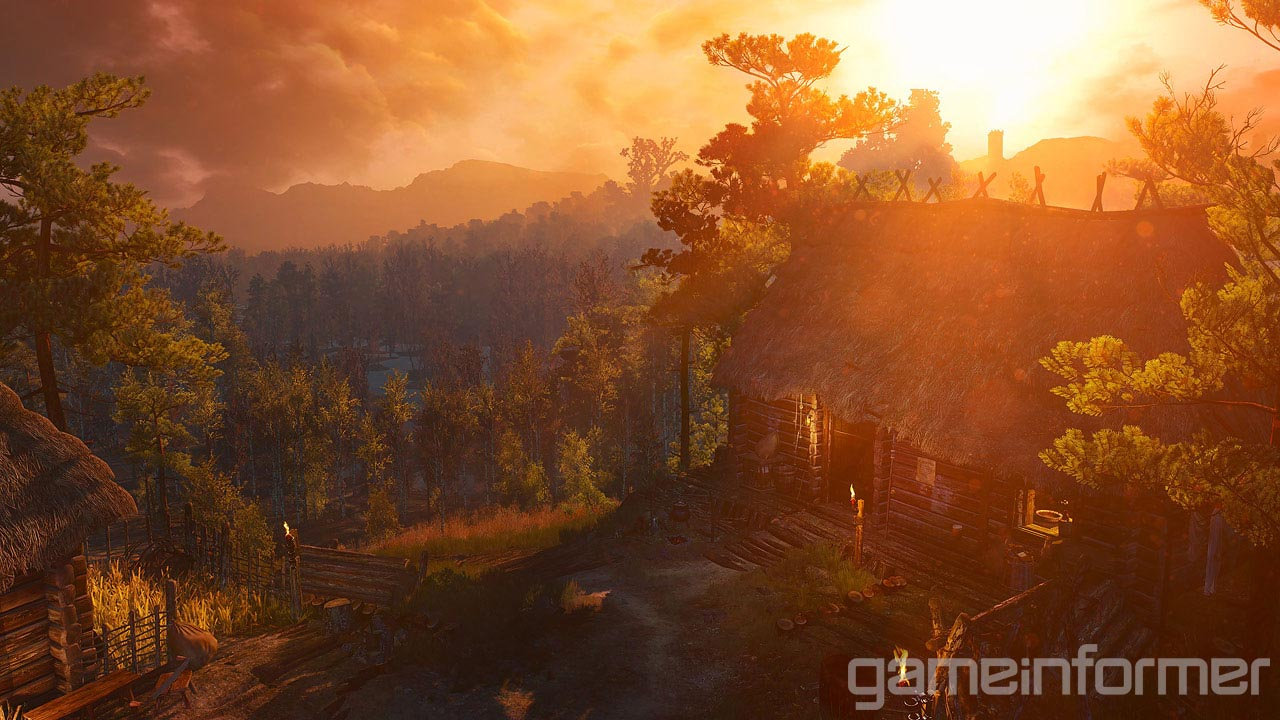
\includegraphics[scale=0.29]{images/einleitung/witcher_weather_1.jpg}
\caption{Grafik in \Fachbegriff{The Witcher 3: Wild Hunt}, Sonnenuntergang \cite{witcher_3_weather}}
\label{fig:witcher_weather_1}
\end{figure}

\begin{figure}[H]
\centering
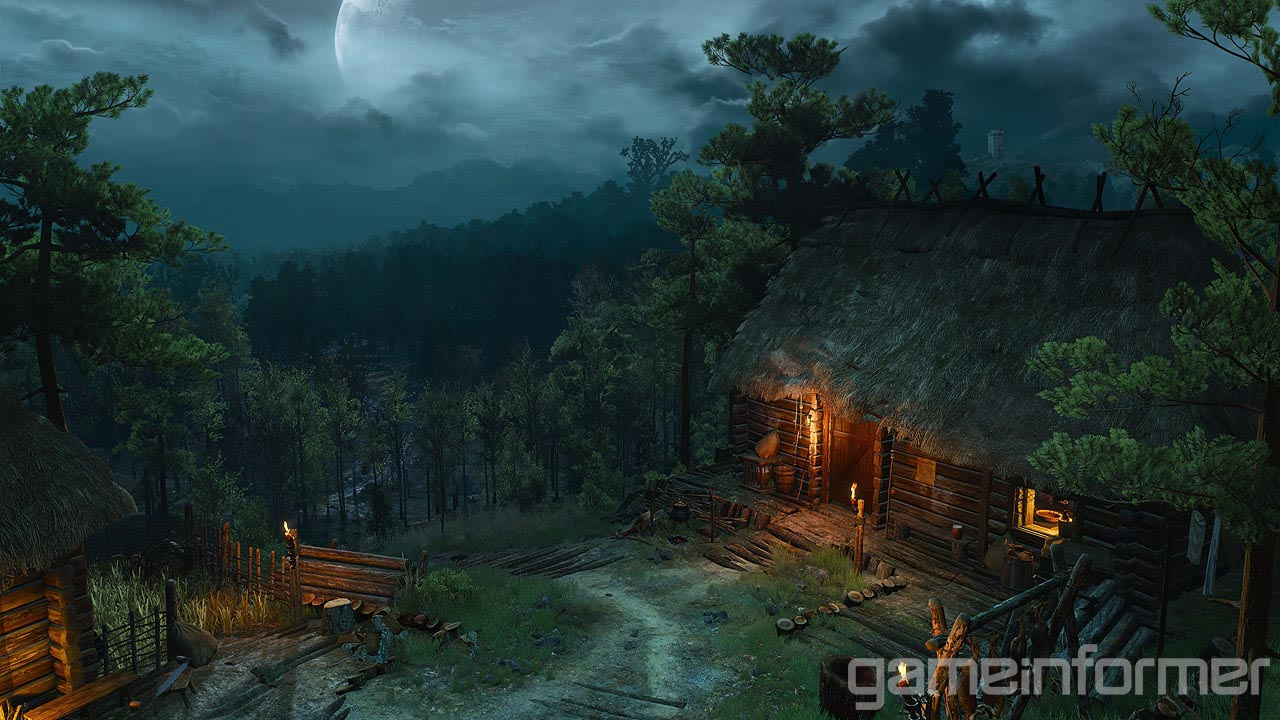
\includegraphics[scale=0.29]{images/einleitung/witcher_weather_2.jpg}
\caption{Grafik in \Fachbegriff{The Witcher 3: Wild Hunt}, Nacht \cite{witcher_3_weather}}
\label{fig:witcher_weather_2}
\end{figure}

Aufgrund der Größe der Städte im Vergleich zu Skyrim muss eine deutlich größere Menge von NPCs verwendet werden. Wegen der höheren Anzahl handelt es sich bei dem Großteil dieser NPCs um namenlose, unbekannte Charaktere. Eine festgelegte Anzahl bekannter NPCs würde hier nicht ausreichen, um die deutlich größere Spielwelt zu füllen. Begibt sich der Spieler an einen Ort, so werden diese Hintergrundcharaktere hinzugefügt und nach dem Verlassen des Ortes wieder entfernt. Diese dienen weniger dem Spielfortschritt sondern der Bevölkerung der Spielwelt. Besonders wegen der Anzahl der Charaktere fällt nicht sofort auf, dass diese stets die gleichen Aktivitäten ausüben. Verfolgt man hingegen einen NPC, so wird schnell ersichtlich, dass sehr einfache Handlungsmuster vorliegen, die sich stets wiederholen. Beispielsweise gehen \acp{npc} endlos zufällig durch die Stadt oder stehen kontinuierlich auf dem Markplatz, anstatt dass sie ihre Aktivitäten zu einem gewissen Zeitpunkt abbrechen, auf ihre Umwelt reagieren und eine neue, sinnvolle Tätigkeit suchen. Dadurch wird die Immersion der Spielwelt verringert. Die Agenten verfügen über keinen sinnvollen Tagesablauf, der mit ihren persönlichen Präferenzen oder Eigenschaften wie ihrem Alter, ihrem Geschlecht oder ihrem Beruf übereinstimmt. Um eine überzeugende Welt darzustellen verfügen Spieler über eine bestimmte Erwartungshaltung, die nicht vollständig erfüllt wird. Beispielsweise sollte ein NPC dem gefolgt wird nach einer gewissen Zeit seinen Wohnort erreichen, sich dann zur Abendzeit schlafen legen und anschließend morgens zur Arbeit gehen.

Die oben beschriebenen statischen Verhaltensmuster lassen sich trotz einer Zunahme der Immersion in anderen Bereichen in den meisten Spielen feststellen. Die vorliegende Arbeit fokussiert sich auf einen Lösungsansatz für diese zugrunde liegende Problematik. Dabei wird der Fokus nicht auf den visuellen Aspekt gelegt, sondern auf das Finden sinnvoller \ac{npc}-Aktionen und dem damit verbundenen Entscheidungsprozess. Ein möglichst menschlich wirkendes Verhalten soll durch eine sinnvolle Auswahl von Tätigkeiten vermittelt werden. Dabei wird ein Machine Learning-Ansatz gewählt, um statt aufwändigem Scripting einen Lernprozess der Agenten anzuregen, sodass weniger manuelle Arbeit nötig ist. Konkret sollen \acp{npc} entwickelt werden, die sich als Hintergrundcharaktere in einer entwickelten Dorfsimulation, um die Spieltwelt lebendig wirken zu lassen.

Das Verhalten der Agenten soll einen sinnvollen Tagesablauf abbilden, der von ihren Attributen, Bedürfnissen und z.B. dem Beruf des \ac{npc} abhängt. Sie erhalten eine Auswahl aus verschiedenen Aktionen, mit denen sie ihre Bedürfnisse befriedigen können, die auf grundsätzlichen menschlichen Bedürfnissen basieren. Dieses Vorgehen wird gewählt, weil gezeigt wurde, dass die Verwendung von menschlichen Eigenschaften wie Bedürfnissen zur Glaubwürdigkeit von Charakteren beitragen können \cite{fallon:believable_background_characters}. Konkret handelt es sich bei den verwendeten Bedürfnissen um interne Funktionen für Eigenschaften wie Hunger, Durst oder Kommunikation. Man spricht von \Fachbegriff{Utility Based Agents} (siehe Abschnitt \ref{utility_agents}). Weiterhin verfügen sie über statische Attribute wie Sportlichkeit, Kommunikationsfreudigkeit oder Intelligenz, die ihre Persönlichkeit definieren sollen. Generell soll dadurch ein möglichst menschliches Verhalten angeregt werden.

Im Folgenden wird kurz die jeweilige Thematik vorgestellt, mit der sich die einzelnen Kapitel der Thesis befassen.

\paragraph{Kapitel \ref{intelligente_agenten} - \nameref{intelligente_agenten}:}
Als erstes behandelt dieses Grundlagenkapitel die Funktionsweise intelligenter Agenten. Dabei werden unterschiedliche typische Verfahren beleuchtet, die für die Entwicklung intelligenter Agenten relevant sind.

\paragraph{Kapitel \ref{reinforcement_learning} - \nameref{reinforcement_learning}:}
\Fachbegriff{Reinforcement Learning} wird als ein Kernkonzept für die Entwicklung lernender Agenten vorgestellt. Zunächst wird dafür auf die generelle Verwendung maschinellen Lernens in Spielen eingegangen. Wichtige Grundlagen wie \Fachbegriff{Markov Decision Problems} werden näher erläutert. Die generelle Funktionsweise sowie der mathematische Hintergrund von modellfreien und modellbasierten Verfahren werden vorgestellt. Weiterhin werden ausgewählte relevante Algorithmen aus dem Bereich, insbesondere der in dieser Arbeit verwendete Algorithmus \ac{ppo}, erläutert. Zuletzt werden Beispiele zum State-of-the-Art von Reinforcement Learning beschrieben.

\paragraph{Kapitel \ref{ml_games_beispiele} - \nameref{ml_games_beispiele}:}
In diesem Kapitel werden verschiedene Anwendungsfälle für Machine Learning in Videospielen beschrieben und in Kategorien eingeteilt. Dabei wird der Fokus nicht nur auf intelligente Agenten, sondern auf generelle Lösungen für die Verbesserung der Authentizität von Spielwelten gelegt. Es soll gezeigt werden, dass es Anwendungsbereiche gibt, in der die Verwendung von Machine Learning Verbesserungen hinsichtlich des Immersionslevels von Spielwelten erzielen kann.

\paragraph{Kapitel \ref{ml_unity} - \nameref{ml_unity}:}
Das Kapitel geht auf die Entwicklung von lernenden intelligenten Agenten innerhalb der Game Engine \Fachbegriff{Unity} ein. Das Hauptthema ist hier die Einführung in das \Fachbegriff{ML-Agents Toolkit}-Framework inklusive der Erläuterung der wichtigsten Konzepte. Zur Veranschaulichung wird ein beispielhaftes Projekt entwickelt und vorgestellt, um wesentliche Aspekte sowie die wichtigsten Komponenten herauszustellen.

\paragraph{Kapitel \ref{entwicklung_dorf} - \nameref{entwicklung_dorf}:}
Der entwickelte Ansatz einer Dorfsimulation mit lernenden, bedürfnisbasierten Agenten wird in diesem Kapitel dokumentiert. Die Anforderungen und generellen Eigenschaften der Simulation werden zunächst beschrieben. Die Architektur des Verfahrens wird anschließend erst generell und dann im Detail vorgestellt. Das Resultat in Form des modellierten Dorfes mit der zugrunde liegenden Architektur sowie den entwickelten Agenten, die sich in der Dorfsimulation bewegen und Aktionen ausführen, werden vorgestellt.

\paragraph{Kapitel \ref{agenten_training} - \nameref{agenten_training}:}
In diesem Kapitel wird der Trainingsvorgang beschrieben, der für den Lernvorgang der Agenten nötig gewesen ist. Dabei wird der Ablauf besprochen, zugrunde liegende Theorien erläutert und Probleme sowie ihre Lösungen gezeigt. Weiterhin werden die Güteüberprüfung des Trainings diskutiert und die Ergebnisse des Trainings vorgestellt. Dabei spielt die Wahl der Hyperparameter sowie die Wahl der Belohnungen der Agenten eine kritische Rolle.

\paragraph{Kapitel \ref{weitere_ansaetze} - \nameref{weitere_ansaetze}:}
Zusätzlich zu dem auf \Fachbegriff{Reinforcement Learning} basierenden Ansatz wurden zwei weitere Verfahren für die Entwicklung intelligenter Agenten genutzt. Zunächst wird die Implementierung dieser Ansätze besprochen. Anschließend werden Unterschiede, Vorteile und Nachteile der drei entwickelten Verfahren untersucht.


\paragraph{Kapitel \ref{fazit} - \nameref{fazit}:}
Schlussendlich wird ein Fazit zur vorliegenden Arbeit getätigt. Es beginnt mit einer rückblickenden Zusammenfassung aller Kapitel. Es wird eine Bewertung der entwickelten Dorfsimulation und den lernenden Agenten vorgenommen. Generelle Probleme mit \Fachbegriff{Machine Learning} und \Fachbegriff{Reinforcement Learning} sowie spezifische Schwierigkeiten, die in der Thesis entstanden sind, werden diskutiert. Ein Ausblick soll schließlich Vorschläge zu Verbesserungsmöglichkeiten und weiterer Forschung geben. 


\chapter{Intelligente Agenten in Videospielen}\label{intelligente_agenten}
\Fachbegriff{Intelligente Agenten} sind autonom handelnde Entitäten, deren Handlungen von bestimmten Zielen abhängen. Sie sammeln Beobachtungen aus einer simulierten oder realen Umgebung, auf deren Basis sie Entscheidungen treffen und die unter Umständen für einen Lernvorgang genutzt werden können. Oft wird dabei auch von \ac{ai} bzw. \ac{ki} gesprochen. Intelligente Agenten werden häufig in Spielen verwendet, um unterschiedliche Arten von \Fachbegriff{Nicht-Spieler-Charakteren} (NPCs) zu simulieren. In der Spielwelt haben diese virtuellen Charaktere in der Regel eine visuelle Repräsentation, beispielsweise anhand einer Person oder eines Tieres, mit der der Spieler interagieren kann. Sie können sowohl eine neutrale Rolle einnehmen (Händler, Dorfbewohner), als auch eine dem Spieler gegenüber feindliche oder freundliche Gesinnung aufweisen (Gegner, Gefährte).

Es gibt eine Vielzahl von Technologien die für die Entscheidungsfindung intelligenter Agenten genutzt werden können. Sowohl die Wahl des Verfahrens als auch der aufgebrachte Aufwand spielen eine kritische Rolle für die Authentizität und die erreichte Intelligenz des Agenten. Im Laufe der Jahre haben diese fortwährend an Komplexität gewonnen. Dabei wird der Versuch unternommen, biologische Verhaltensmuster nachzuahmen, um eine Art von pseudo-intelligentem Verhalten zu erschaffen. Die Definition von \textit{Intelligenz} oder \Fachbegriff{künstlicher Intelligenz} ist dabei allerdings unpräzise, da es keine allgemeingültige Definition gibt.

Nach Russel und Norvig \cite{art_int_mod_app} könnte bereits eine simple Maschine wie ein Thermostat als intelligenter Agent bezeichnet werden, da er eigenständig auf äußere Einflüsse reagiert. Laut dieser Definition könnten auch Software-Agenten wie Mining-Bots, die scheinbar eigenständig Daten sammeln, als intelligente Agenten bezeichnet werden. Nikola Kasabov \cite{kasabov} bietet hingegen eine vollkommen andere  Definition intelligenter Agenten anhand einer Menge von Anforderungen an den Agenten:

\begin{itemize}
    \item Regeln für Problemlösungen müssen inkrementell angepasst werden.
    \item Die Anpassung muss in Echtzeit stattfinden.
    \item Eine Selbstanalyse bezüglich des Verhaltens und des Erfolgs muss stattfinden.
    \item Ein Lernvorgang durch Interaktion mit der Umgebung muss gegeben sein.
    \item Der Lernvorgang muss mit einer ausreichenden Datenmenge schnell ablaufen.
    \item Es muss ein Gedächtnis vorhanden sein.
    \item Parameter für die Realisierung von Kurz- und Langzeitgedächtnis sowie das Vergessen von Erinnerungen müssen gegeben sein.
\end{itemize}

Kein intelligenter Agent in einem Spiel ist bisher in der Lage, diesen Anforderungen gerecht zu werden. Alternative Definitionen gehen in der Regel nicht über die Anforderung hinaus, dass der Agent selbst handeln muss.

Der Begriff \Fachbegriff{Intelligenter Agent} wird daher im Folgenden stets als Software-Agent in Umfeld einer simulierten Realität anhand von Videospielen definiert, der selbst Entscheidungen trifft. Ziel dieses Agenten ist eine sinnvolle Entscheidungsfindung zwecks einer Interaktion mit dem Spieler. Dabei soll so weit wie möglich eine scheinbare Imitation menschlichen Verhaltens umgesetzt werden, es werden allerdings keine weiteren Anforderungen an Lernvorgänge oder ein Gedächtnis gestellt. Dafür kann eine analytische, formale Vorgehensweise der Verfahren für die Entwicklung von Algorithmen für Agenten verwendet werden. Alternativ wird der Versuch unternommen, biologische oder kognitive Prozesse zu imitieren, um intelligentes Verhalten zu simulieren. Unabhängig von der gewählten Technologie soll lediglich der Eindruck von Intelligenz erweckt werden, ohne dass dabei tatsächliche Intelligenz erreicht werden muss. Die von Kasabov definierten Kriterien bezüglich eines Lernvorgangs oder einem Gedächtnisvermögen etc. sind daher nur optionale Eigenschaften.
Im folgenden Abschnitt werden einige etablierte Methoden für die Entscheidungsfindung intelligenter Agenten vorgestellt.


\section{Finite State Machines}
Bei \Fachbegriff{Finite State Machines} oder \Fachbegriff{Endlichen Automaten} handelt es sich um abstrakte Zustandsmaschinen, die sich in jeweils einem von mehreren Zuständen befinden können \cite{ai_for_game_devs} \cite{rich_basic_game_ai_course} \cite{cmsc_425} \cite{state_machine_flora_game} \cite{game_ai_by_example}. Das Ziel des Verfahrens ist eine reduzierte Abbildung der Wirklichkeit anhand eines Modells, welches durch die State Machine beschrieben wird. Die State Machine stellt also nur den Ansatz einer Simulation der Wirklichkeit dar, sowie auch alle weiteren vorgestellten Technologien für intelligente Agenten. Dafür müssen Zustände und Zustandsübergänge bzw. \Fachbegriff{States} und \Fachbegriff{Transitions} definiert werden. Die Zustandsübergänge schaffen Verbindungen in andere Zustände und werden durch bestimmte Konditionen gestartet, sogenannte \Fachbegriff{Trigger}. Ein populäres Beispiel für Spiele, in denen State Machines zum Einsatz kommen, ist das 1992 veröffentliche \Fachbegriff{Wolfenstein 3D} \cite{wolfenstein}.

\begin{figure}[H]
\centering
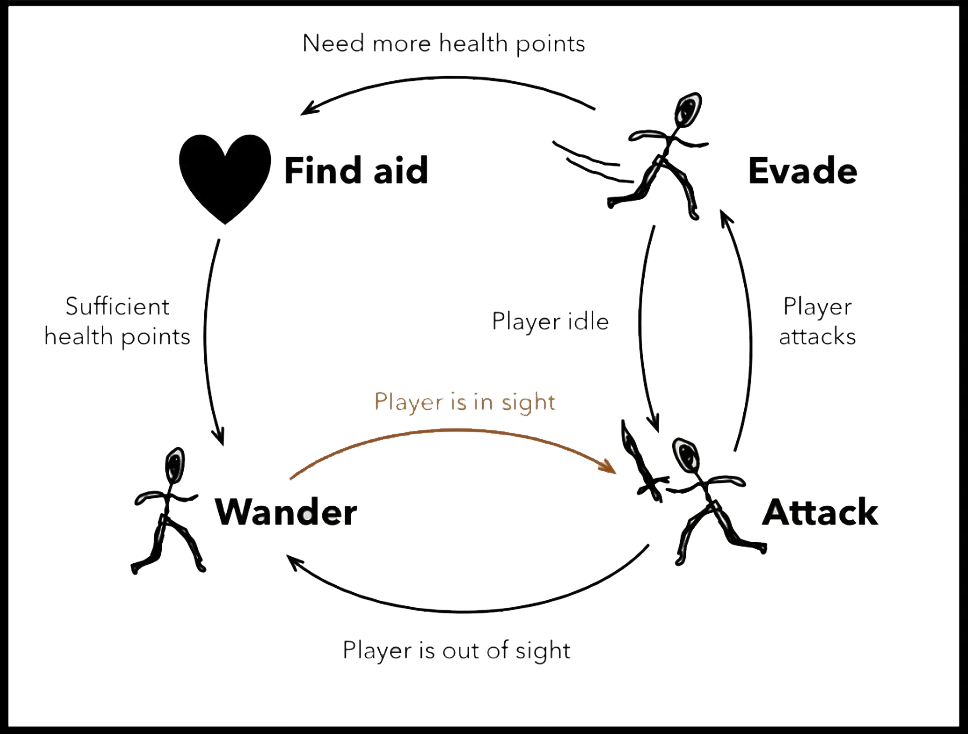
\includegraphics[scale=0.3]{images/chapter_2_int_agents/state_machine.png}
\caption{Beispielhafte Finite State Machine \cite{art_int_vid_games_towardsdatascience}}
\label{fig:state_machine_1}
\end{figure}

Die Abbildung \ref{fig:state_machine_1} zeigt eine Finite Sate Machine anhand eines simplifizierten Beispiels. Es werden die Zustände \aufzaehlung{Find aid}, \aufzaehlung{Wander}, \aufzaehlung{Attack} und \aufzaehlung{Evade} für einen NPC definiert. Wenn der NPC sich im \textit{Wander}-Zustand befindet, so kann er lediglich in den \textit{Attack}-Zustand wechseln. Der Trigger dafür ist die Sichtbarkeit des Spielers. Sobald die Triggerkondition eintrifft, findet ein Zustandsübergang in den \textit{Attack}-Zustand statt. Für diesen Zustand gibt es nun zwei mögliche Zustandsübergänge: Wenn der Spieler ebenfalls angreift, so wechselt der NPC in den \textit{Evade}-Zustand und versucht, vor dem Spieler zu flüchten. Wenn der Spieler außer Sicht ist, wechselt er zurück in den \textit{Wander}-Zustand. Aus dem \textit{Evade}-Zustand heraus kann der NPC zurück in den \textit{Attack}-Zustand wechseln, wenn der Spieler sich im \Fachbegriff{Idle}-Modus befindet, also nichts tut. Weiterhin wechselt der NPC in den \textit{Find Aid}-Zustand, sobald seine Lebenspunkte unter einem bestimmten Wert liegen. Wenn seine Lebenspunkte aufgefüllt wurden findet ein Zustandsübergang in den \textit{Wander}-Zustand statt.

Die folgenden Codebeispiele (siehe Listings \ref{lst:fsm_state} bis \ref{lst:fsm_getactions}) zeigen eine mögliche minimalistische Implementierung der State Machine: 

\begin{tabular}{ll}
\begin{minipage}{.48\textwidth}
\begin{lstlisting}[linewidth=7.25cm, label=lst:fsm_state, caption=State Class, xleftmargin=1.9cm]
class State {
    var action;
    var entryAction;
    var exitAction;
    var transitions;
}
\end{lstlisting}
\end{minipage}
\hfill

\begin{minipage}{.48\textwidth}
\begin{lstlisting}[linewidth=7.25cm, label=lst:fsm_transition, caption=Transition Class, xleftmargin=1.7cm]
class Transition {
    var state;
    function isActive;
}
\end{lstlisting}
\end{minipage}
\end{tabular}

\begin{minipage}{\linewidth}
\begin{lstlisting}[linewidth=16.4cm, label=lst:fsm_example-state, caption=Beispiel-State, xleftmargin=1cm]
class AttackState extends State {
  var action = new AttackAction();
  var entryAction = new MoveAndDrawSwordAction();
  var exitAction = new SheathSwordAction();
  var transitions = [new WanderAttackTransition(),
    new EvadeAttackTransition()];
}
\end{lstlisting}
\end{minipage}

\begin{minipage}{\linewidth}
\begin{lstlisting}[linewidth=16.4cm, label=lst:fsm_example-transition, caption=Beispiel-Transition, xleftmargin=1cm]
class WanderAttackTransition extends Transition {
  var state = new AttackState();
  function isActive() {
    return isPlayerClose();
  }
}
\end{lstlisting}
\end{minipage}

\begin{minipage}{\linewidth}
\hspace{2cm} \begin{lstlisting}[linewidth=16.4cm, label=lst:fsm_getactions, caption=State Machine Controller, xleftmargin=1cm]
class StateController {
    [...]

    function getActions() {
        activeTransition = null;
        foreach (transition in currentState.transitions) {
            if (transition.isActive()) {
                activeTransition = transition;
                break;
            }
        }
        if (activeTransition != null) {
            newState = activeTransition.state;
            actions += currentState.exitAction;
            actions += newState.entryAction;
            actions += newState.action;
            currentState = newState;
            return actions;
        } else return [currentState.action];
    }
}
\end{lstlisting}
\end{minipage}

Zunächst werden die Klassen \inlinecode{State} und \inlinecode{Transition} definiert. \inlinecode{State} benötigt die ausführbare Hauptaktion \inlinecode{action}, sowie eine Eingangs- und Ausgangsaktion, wie beispielsweise eine bestimmte Animation, die für einen flüssigen Übergang der Zustände ausgeführt wird. Für den Zustand \inlinecode{AttackState} werden daher entsprechende Aktionen für das Aufnehmen sowie Verstauen eines Schwertes definiert. Die Hauptaktion \inlinecode{AttackAction} sorgt dafür, dass eine Attacke ausgeführt wird. Weiterhin werden zwei Zustandsübergänge \inlinecode{WanderAttackTransition} und \inlinecode{EvadeAttackTransition} definiert, da der \ac{npc} entweder aus dem \Fachbegriff{Wander}- oder aus dem \Fachbegriff{Evade}-Zustand in den \Fachbegriff{Attack}-Zustand wechseln kann.
Jede Transition verfügt dabei über den Zielzustand und über eine Funktion \texttt{isActive}, die angibt, ob die Transition aktiv ist. Die \texttt{WanderAttackTransition} definiert daher \texttt{AttackState} als Zielzustand und prüft innerhalb von \texttt{isActive}, ob ein Spieler in der Nähe ist.
Der \texttt{StateController} prüft nun mittels der Funktion \texttt{getActions} in regelmäßigen Abständen oder nach dem Ausführen von Einzelaktionen durch das Aufrufen der \texttt{isActive}-Funktionen für alle Transitions, ob neue Zustandsübergänge verfügbar sind. Sobald eine solche gefunden wird, wird der neue Zustand gesetzt und sowohl die Ausgangsaktion des aktuellen Zustands, sowie die Eingangs- und die Hauptaktion des neuen Zustands werden in die Liste der auszuführenden Aktionen aufgenommen. Ansonsten wird stets die Hauptaktion des aktuellen Zustands weiterhin ausgeführt.

Nach diesem einfachen Schema werden Zustände und ihre Übergänge definiert. Der \Fachbegriff{StateController} stellt anschließend sicher, dass Zustandsübergänge automatisch eingeleitet werden. In diesem Beispiel wird immer der erste mögliche Zustandsübergang genommen, theoretisch könnte man den Übergängen nun aber Prioritäten zuweisen. Die Architektur und das Anlegen neuer Zustände sind simpel und effizient. Bei der Darstellung aller möglichen Zustände eines echten, komplexen Spiels werden jedoch schnell Grenzen erreicht, da eine hohe Menge von Zuständen und Übergängen erreicht wird. Aufgrund des hohen Determinismus von State Machines in ihrere einfachen Form eignen sie sich weiterhin nicht für den Einsatz in jedem Spiel. Man stelle sich ein Strategiespiel vor, in dem State Machines für NPC-Gegner verwendet werden. Diese Gegner würden jedes Mal auf die gleiche Art und Weise auf bestimmte Situationen reagieren. Das ist zum einen problematisch, weil dadurch statt einem authentischen, dynamischen Verhalten lediglich eine repetitive Spielerfahrung zustandekommt und zum anderen, weil derartiges Verhalten vorhersehbar ist und daher leicht durch den Spieler ausgenutzt werden kann.


\paragraph{Hierarchical State Machines}
% https://www.cs.umd.edu/class/spring2019/cmsc425/handouts/lect21-ai-dec-making.pdf
State Machines haben zusätzlich das Problem, dass die Anzahl der Zustände schnell große und daher unübersichtliche Ausmaße annehmen kann. Außerdem ist es nur möglich, einen einzelnen Zustand zur Zeit einzunehmen, wodurch nur sehr eingeschränktes Verhalten realisiert werden kann. Möchte man beispielsweise modellieren, dass ein NPC zur selben Zeit verwundet ist und gleichzeitig den Spieler angreift, muss dafür ein eigener neuer Zustand \Fachbegriff{IsAttackingWhileWounded} entworfen werden. Wenn man erreichen will, dass der Spieler in jedem bereits entworfenen Zustand ebenfalls verwundet sein kann, muss dann eine Vielzahl neuer Zustände entworfen werden. So resultiert die Kombination aus allen möglichen Zuständen für die Erstellung neuer Sub-Zustände und Sub-Transitions oft in vollkommen unbrauchbaren Zustandsmengen, die nicht mehr verwaltet werden können.

Eine mögliche Lösung für diese Probleme ist die Entwicklung von State Machines in einer hierarchischen Struktur. Dafür gibt es eine Anzahl von \Fachbegriff{High-Level}-Zuständen, die einen allgemeinen, übergeordneten Kontext für das Charakterverhalten darstellen. In jedem dieser High-Level-Zuständen gibt es dann mehrere \Fachbegriff{Sub-Level}-Zustände, die für spezifischeres Verhalten sorgen. Solche Systeme werden als \Fachbegriff{Hierarchical State Machines} bezeichnet \cite{cmsc_425}. Die Struktur des Verfahrens lässt gewisse Gemeinsamkeiten zu UML-Diagrammen erkennen, in denen ebenfalls hierarchisch geschachtelte Gruppen von Aktionen gebildet werden.

Als weiteres Beispiel wird ein Agent angeführt, der die Zustände \aufzaehlung{On Guard}, \aufzaehlung{Fight} und \aufzaehlung{Run Away} mit Transitions untereinander besitzt. Jetzt soll ein neuer Zustand \aufzaehlung{Get Food} eingeführt werden, der zu jeder Situation eintreten kann, sobald der Agent hungrig ist. Von jedem möglichen Zustand müsste dann ein Übergang zu dem neuen Zustand geschaffen werden (siehe Abbildung \ref{fig:hierchical_state_machine_bot_1}).

\begin{figure}[H]
\centering
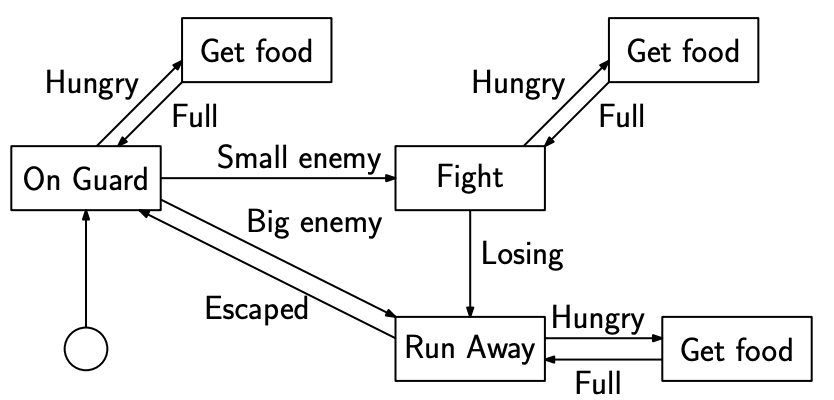
\includegraphics[scale=0.74]{images/chapter_2_int_agents/hierarchical_state_machine_1_without.png}
\caption{Hinzufügen eines neues Zustands, normale State Machine}
\label{fig:hierchical_state_machine_bot_1}
\end{figure}

\begin{figure}[H]
\centering
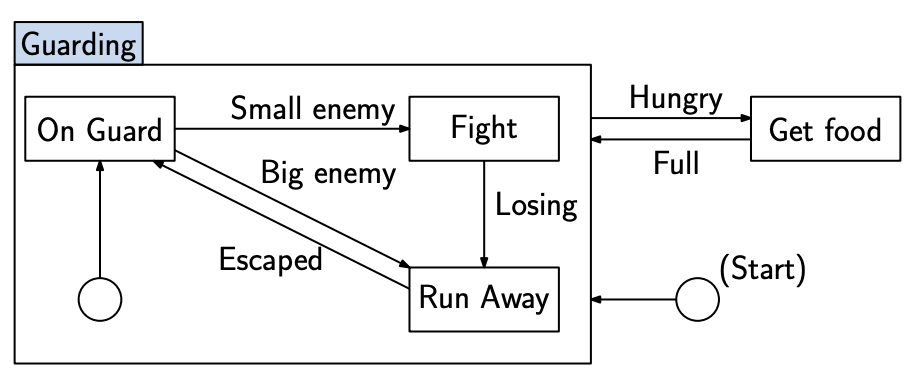
\includegraphics[scale=0.7]{images/chapter_2_int_agents/hierarchical_state_machine_2_with.png}
\caption{Hinzufügen eines neues Zustands, hierarchische State Machine}
\label{fig:hierchical_state_machine_bot_2}
\end{figure}

Abbildung \ref{fig:hierchical_state_machine_bot_2} zeigt den gleichen Vorgang des Ergänzens um einen weiteren Zustand mit einer hierarchischen State Machine, statt einer herkömmlichen. Es wird ein neuer High-Level-State \Fachbegriff{Guarding} gebildet, der die bereits vorhandenen Zustände enthält. Dieser neue \sogenannt{Super-State} verfügt nun über einen Startpunkt, der nur dann angesprochen wird, wenn man das erste mal den Super-State betritt. Die Zustandsübergänge von jedem Sub-Zustand des Super-States sind implizit gegeben. Das könnte beispielsweise funktionieren, indem ein Stack verwendet wird, der die aktiven Zustände nach ihren Level sortiert, sodass der Zustand mit dem höchsten Level immer an der ersten Stelle des Stacks steht. Um mögliche Transitions zu prüfen, würde dann vom letzten bis zum ersten Element geprüft werden, ob ein Zustand für die bestimmte Aktion verfügbar ist \cite{cmsc_425}.

Die Architektur der State Machine wird dadurch simplifiziert und modularisiert, da insgesamt deutlich weniger Zustände verwaltet und erzeugt werden müssen. Weiterhin können insgesamt mehr Zustände verarbeitet werden, weil die Transitions vieler Zustände automatisch implizit definiert werden.



\section{Decision Trees}
% unreal tournament 2004: https://www.researchgate.net/publication/221308927_Decision_Tree-Based_Algorithms_for_Implementing_Bot_AI_in_UT2004
Ein klassisches Verfahren für die Entscheidungsfindung intelligenter Agenten beruht auf der Verwendung von \Fachbegriff{Decision Trees}. Dabei wird eine einfache Baumstruktur aus möglichen Entscheidungen gebildet. Genauer handelt es sich um einen gewurzelten Baum. Häufig findet man binäre Bäume vor. Das Verfahren ist besonders sinnvoll, wenn der Agent aus vielen mögliche Entscheidungen zur selben Zeit auswählen muss. Je nachdem welche Entscheidung gewählt wurde, öffnet sich ein neuer Zweig des Baumes, unter Umständen mit weiteren Entscheidungen und möglichen Abstiegen.
Die Knoten des Baumes werden als \sogenannt{Decision Point}, also \Fachbegriff{Entscheidungsknoten}, bezeichnet. Jeder Entscheidungsknoten prüft eine bestimmte binäre Bedingung, beispielsweise: \textit{Ist der Spieler sichtbar?}. Damit wird eine Bedingung für den Abstieg des Baumes aufgestellt. Die Antwort auf die Bedingung ist dafür verantwortlich, ob ein Abstieg in den linken oder rechten Zweig des Entscheidungsknotens erfolgt. Bei einem binären Baum handelt es sich um \sogenannt{Ja-oder-Nein}-Fragen. Abbildung \ref{fig:decision_tree_1} zeigt ein Beispiel für einen typischen, stark simplifizierten Entscheidungsbaum für einen kämpfenden NPC.

\begin{figure}[H]
\centering
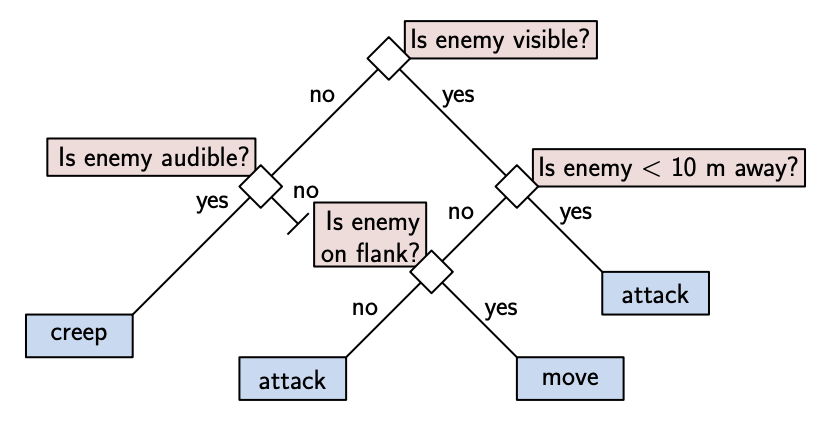
\includegraphics[scale=0.85]{images/chapter_2_int_agents/decision_tree_example_1.png}
\caption{Beispielhafter Decision Tree \cite{cmsc_425}}
\label{fig:decision_tree_1}
\end{figure}

% beispiele? besonderheiten?
% man könnte heir die erweiterten bäume mit aufnehmen..
% https://www.cs.umd.edu/class/spring2019/cmsc425/handouts/lect21-ai-dec-making.pdf


Decision Trees sind einfach zu verstehen und können leicht implementiert werden. Zusätzlich bieten sie eine hohe Performanz. Neben der Entscheidungsfindung von NPCs haben sie noch weitere Anwendungsbereiche in Videospielen. Beispielsweise werden Bäume für Questsysteme eingesetzt. Das Spiel \Fachbegriff{Witcher 3} \cite{witcher_3} verwendet beispielsweise Decision Trees, um je nach den Handlungen des Spielers im Spiel den Ablauf vom Ende des Spiels festzulegen.

% Monte Carlo search trees
% https://towardsdatascience.com/artificial-intelligence-in-video-games-3e2566d59c22



\section{Behavior Trees}
\Fachbegriff{Behavior Trees} sind eine Weiterentwicklung von Finite State Machines, bei der Baumstrukturen genutzt werden. Sie gehen von einem modularen komponentenbasierten System für das Verhalten bzw. \textit{Behavior} von Agenten aus und verwendet dafür gewurzelte Bäume \cite{cmsc_425} \cite{ai_for_game_devs} \cite{gamasutra_behavior_tree}. Der erste Einsatz von Behavior Trees erfolgte im Jahr 2004 im erfolgreichen Spiel \Fachbegriff{Halo 2} \cite{halo_behavior_tree_gdc} \cite{halo_2}.
Ein beispielhafter Behavior Tree ist in Abbildung \ref{fig:behavior_tree_1} zu sehen.

\begin{figure}[H]
\centering
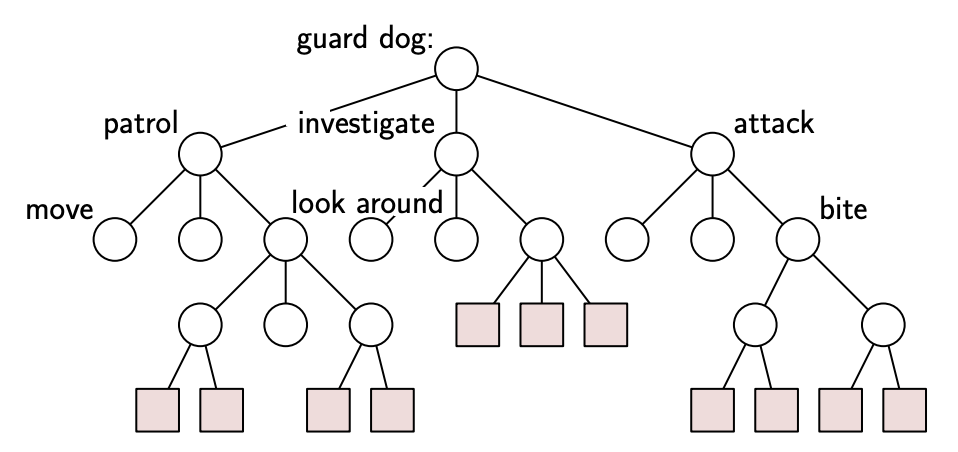
\includegraphics[scale=0.8]{images/chapter_2_int_agents/behavior_tree_1.png}
\caption{Beispielhafter Behavior Tree \cite{cmsc_425}}
\label{fig:behavior_tree_1}
\end{figure}

Die Knotenpunkte des Baumes enthalten sogenannte \Fachbegriff{Tasks} - spezifische Aufgaben, die ein explizites Ziel verfolgen. Tasks besteht aus einer Menge von Konditionen die bestimmen, welcher Task aktiv ist, sowie Aktionen, die die Ausführung des Tasks enkodieren. Da Tasks fehlschlagen können, geben diese bei der Ausführung einen von drei Statusberichten an: \textit{Running}, \textit{Success} oder \textit{Failure}. Alle im Baum enthaltenen Tasks sind Akteuren des Spiels zugewiesen. Die Granularität der Tasks erhöht sich mit steigender Tiefe des Baumes. Jeder Task beschreibt dabei ein Sub-Verhalten, das eine bestimmte Aufgabe im Kontext des übergeordneten Knotens übernimmt. Die Wurzel des Baumes beschreibt das generelle Verhalten für eine bestimmte Entität. Sie könnte beispielsweise das Verhalten \Fachbegriff{Gegner} oder \Fachbegriff{Wachhund} darstellen. 
Einzelne Top-Level-Tasks (Knoten direkt unter der Wurzel) beschreiben allgemeines Verhalten, wie beispielsweise \aufzaehlung{Angreifen}, \aufzaehlung{Umschauen} oder \aufzaehlung{Patroullieren}. Die Sub-Tasks von \textit{Angreifen} könnten zum Beispiel \textit{Schlagen} oder \textit{Schießen} sein.

Die Blätter des Baumes beschreiben die tatsächliche Interaktion der Entität mit dem Spiel und die Ausführung von Aktionen. Sie beinhalten Konditionen, die erfüllt sein müssen, und Aktionen, die dann ausgeführt werden. Für das Beispiel des Wachhundes könnten die Konditionen den Zustand des Hundes (\textit{Ist der Hund hungrig? Ist der Hund verletzt?}) oder den allgemeinen Spielzustand betreffen (\textit{Ist ein Gegner in der Nähe?}). Die mit den Konditionen verbundenen Aktionen verändern dann dessen Zustand - der Hund könnte beispielsweise den Spieler beißen und seine Lebenspunkte verringern oder einfach eine Animation abspielen. Die Konditionen können auch als Filter betrachtet werden, die bestimmen, welche Aktionen ausgeführt werden\cite{cmsc_425}.


\paragraph{Task Composition}
Behavior Trees bieten verschiedene Möglichkeiten für die Komposition von Tasks. Typischerweise werden Tasks entweder sequentiell oder ausgewählt abgearbeitet.

Bei der sequentiellen Ausführung von Tasks wird eine Liste von Tasks nacheinander verarbeitet (\Fachbegriff{Sequences}). Sobald ein Task fehlschlägt, wird die Sequenz terminiert. Eine beispielhafte Ausführung wird anhand der Abbildung \ref{fig:behavior_tree_2} verdeutlicht. Der Pfeil in der Grafik steht für die sequenzielle Ausführung der Aktionen.

\begin{figure}[H]
\centering
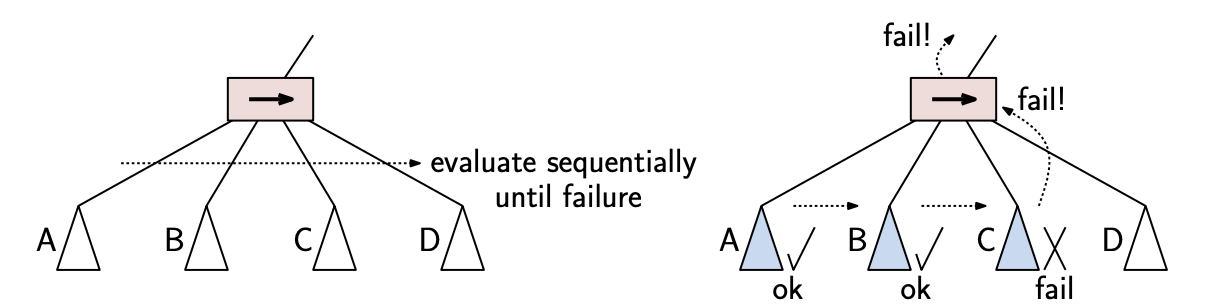
\includegraphics[scale=0.75]{images/chapter_2_int_agents/behavior_tree_2.png}
\caption{Sequenzielle Ausführung in Behavior Tree \cite{cmsc_425}}
\label{fig:behavior_tree_2}
\end{figure}

Bei der ausgewählten Ausführung (\Fachbegriff{Selector}) wird maximal ein Task aus einer Menge von Tasks ausgewählt. Sobald der erste Task einen erfolgreiche Statusbericht versendet, wird die Ausführung terminiert. Abbildung \ref{fig:behavior_tree_3} zeigt eine beispielhafte ausgewählte Ausführung. Das Fragezeichen verdeutlicht in der Abbildung den Selector, eine ausgewählte Ausführung bis zum ersten Erfolg.

\begin{figure}[H]
\centering
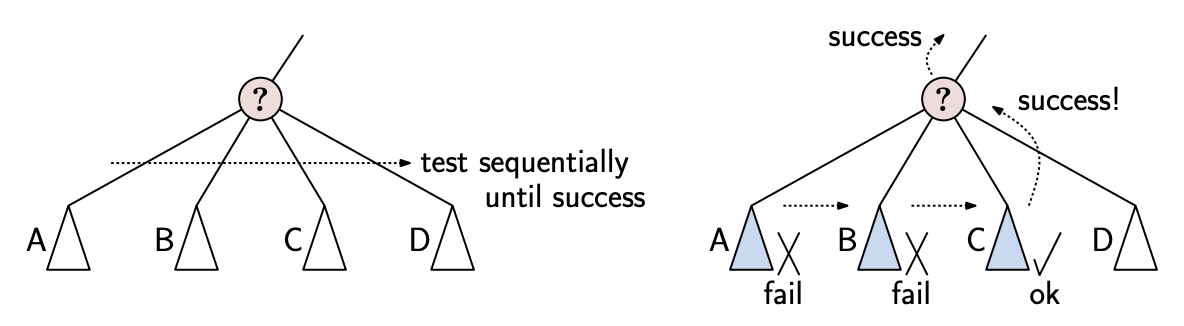
\includegraphics[scale=0.75]{images/chapter_2_int_agents/behavior_tree_3.png}
\caption{Ausgewählte Ausführung in Behavior Tree \cite{cmsc_425}}
\label{fig:behavior_tree_3}
\end{figure}

Mit Sequences und Selector werden den Behavior Trees einige Möglichkeiten hinzugefügt, die für Finite State Machines nicht verfügbar sind. Sequences und Selector können kombiniert werden, um ein komplexeres Verhalten zu realisieren. Einzelne Teilbäume dieses Verhaltens können dann auf Sequences und andere Teilbäume auf Selector basieren.
In Abbildung \ref{fig:behavior_tree_4} ist ein konkretes Beispiel für eine Kombination von Selector und Sequence zu erkennen, in dem ein NPC auf verschiedene Art und Weise je nach Beschaffenheit des Spielzustands versucht, in einen Raum zu gelangen. Anhand der Symbole in der Grafik (\sogenannt{!} und \sogenannt{?}) ist die Kombination von Selector und Sequence erkennbar. Der Agent betritt unmittelbar den Raum, wenn die Tür offen ist. Falls dies nicht gelungen ist, bewegt er sich zunächst zur Tür und versucht anschließend, diese zu öffnen. Wenn auch dies scheitert, wird die Tür aufgebrochen, sodass der Agent schlussendlich den Raum betreten kann.

\begin{figure}[H]
\centering
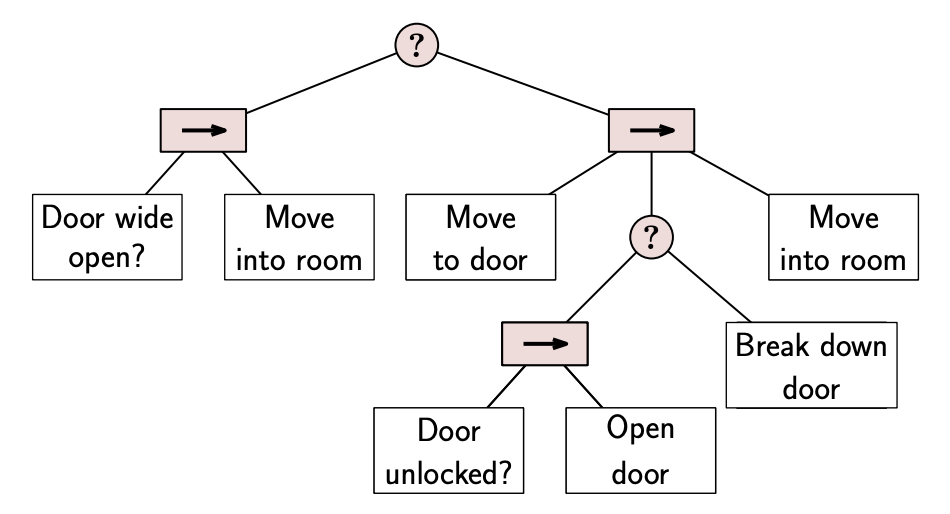
\includegraphics[scale=0.75]{images/chapter_2_int_agents/behavior_tree_4.png}
\caption{Kombination sequenzieller und ausgewählter Ausführung in Behavior Tree \cite{cmsc_425}}
\label{fig:behavior_tree_4}
\end{figure}

Aus der Sicht des Software-Engineering werden dem Programmierer mit Behavior Trees ein besser strukturierter Kontext für die Entwicklung von Verhalten zur Verfügung gestellt \cite{cmsc_425}. Da sie alle Vorteile von Finite State Machines bieten und darüber hinaus über eine hohe Performanz verfügen, sind Behavior Trees zu einer sinnvollen Alternative zu State Machines geworden \cite{behavior_tree_article}. Sie werden daher zunehmend in großem Maßstab in erfolgreichen und komplexen Spielen wie \Fachbegriff{Halo}, \Fachbegriff{Bioshock} oder \Fachbegriff{Spore} verwendet \cite{behavior_tree_wiki}.




\section{Goal Oriented Action Planning (GOAP)}\label{goap}
\ac{goap} ist ein System für die Planung und Ausführung von Aktionen für einen Agenten und wurde zunächst für das Spiel \Fachbegriff{F.E.A.R.} entwickelt \cite{goap_fear}. Es erlaubt einem Agenten die Planung einer Sequenz von Aktionen zum Erreichen eines bestimmten Ziels. GOAP bietet gegenüber Finite State Machines den Vorteil, dass keine großen Mengen von Zuständen und Zustandsübergängen definiert werden müssen \cite{goap_gamedevelopment} \cite{game_ai_by_example}. Anstelle von Zuständen werden hier modulare, voneinander entkoppelte Aktionen verwendet \cite{goap_haw}.

GOAP verlangt für die Entscheidungsfindung lediglich die Definition von \Fachbegriff{Goals} und \Fachbegriff{Aktionen} \cite{ai_for_game_devs}. Goals sind festgelegte Konditionen, die ein Agent erfüllen möchte. Um ein Goal zu erreichen, werden Aktionen ausgeführt, die den Spielzustand verändern. Eine Kette aus Aktionen wird aufgebaut, die den Spielzustand so verändern, dass die Konditionen des Goals erfüllt sind. Bei einer Aktion kann es sich beispielsweise um das simple Öffnen einer Tür oder das Aufnehmen eines Gegenstands in das Inventar des NPCs handeln. Die vom Agenten ausgeführten Aktionen haben jeweils eine Menge von Bedingungen (\Fachbegriff{Preconditions}), die für die Ausführung der Aktion vorausgesetzt werden, sowie eine Menge von Effekten als eine Folge der Aktion. Diese sorgen dafür, dass die Bedingung eines Goals schlussendlich erfüllt wird.

Aus den einzelnen Aktionen erstellt der sogenannte \Fachbegriff{GOAP Planner} eine Sequenz zum Erreichen eines Ziels. Es handelt sich um eine zentrale Verwaltungs- und Planungseinheit für die Ausführung von Aktionen im GOAP-System. Der GOAP Planner kennt die Bedingungen der Goals sowie die Preconditions und Effekte der Aktionen. Auf dieser Grundlage ist er in der Lage zu erkennen, welche Effekte welcher Aktionen benötigt werden, um das Goal zu erreichen. Dadurch kennt der GOAP Planner auch die Preconditions der benötigten Aktionen und kümmert sich ebenfalls darum, dass diese Bedingungen erfüllt werden. Dafür werden unter Umständen weitere Aktionen in die Sequenz eingefügt. Der Planner stellt sicher, dass die benötigten Ketten von Aktionen in der richtigen Reihenfolge ausgeführt werden.
Konkret sucht der GOAP Planner zunächst nach allen vorhandenen Goals. Für diese erstellt er rückwärts vom Goal aus gehend eine Baumstruktur. Diese besteht aus allen möglichen Sequenzen von Aktionen, die zum jeweiligen Ziel führen. Dabei wird der jeweils kürzeste Weg gewählt, der zum Ziel führt. Die Pläne des Agenten sind nicht statisch, sondern werden erst zur Laufzeit generiert, sodass dieser sich dynamisch an die jeweiligen Umstände seiner Umgebung anpassen kann. In der Abbildung \ref{fig:goap_1} ist eine beispielhafte Sequenz in einem GOAP-System zu erkennen.

\begin{figure}[H]
\centering
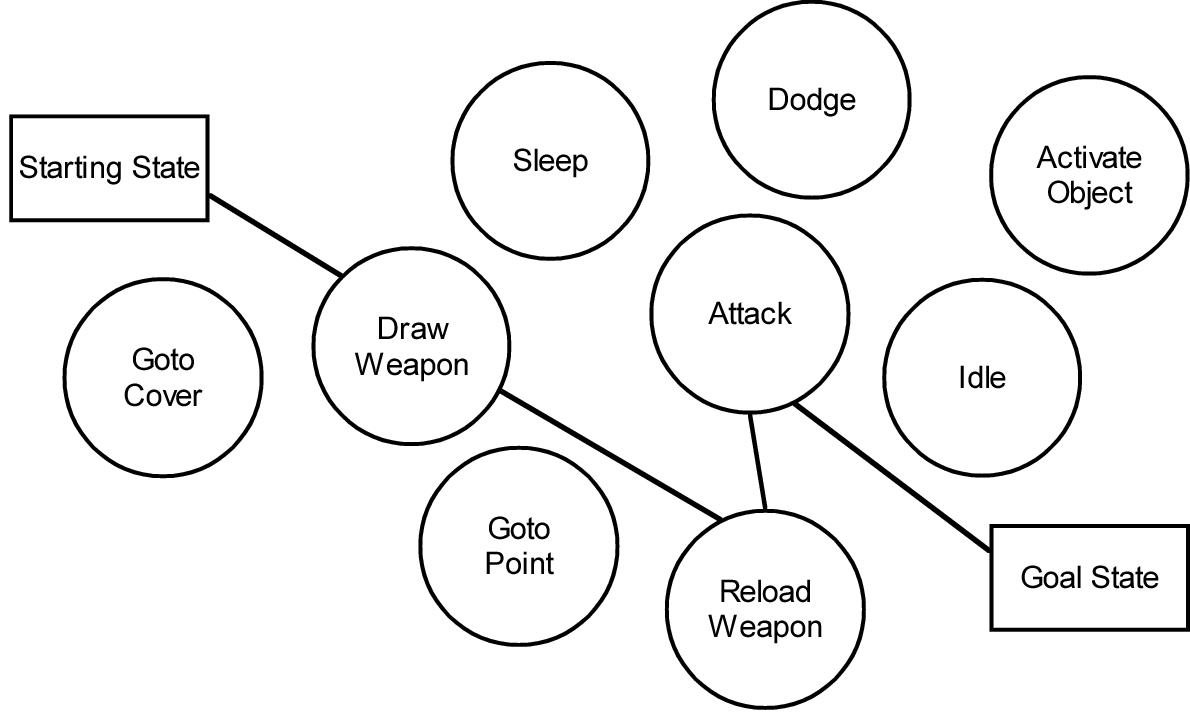
\includegraphics[scale=0.25]{images/chapter_2_int_agents/goap_1.png}
\caption{GOAP-Sequenz nach Orkin \cite{goap_fear}}
\label{fig:goap_1}
\end{figure}

Es sei darauf geachtet, dass keine Übergänge zwischen den Aktionen vorhanden sind. Die Abbildung zeigt das GOAP-Äquivalent einer State Machine mit übergangslosen Aktionen statt Zuständen und Transitions.
Intern verwendet GOAP eine minimale State Machine, die über drei Zustände verfügt: \aufzaehlung{Idle}, \aufzaehlung{MoveTo} und \aufzaehlung{PerformAction}. Das ist notwendig, da sich der Agent für einige Aktionen in der Nähe eines bestimmten Objekts befinden muss. Das Bewegen des Agenten ist nicht Teil des eigentlichen GOAPs, weil sonst viele zusätzliche Aktionen für die Bewegung zu bestimmten Zielen von Aktionen definiert werden müssten. Stattdessen kann jeder Aktion bei Bedarf ein Ziel zugewiesen werden.
Im \Fachbegriff{Idle}-Zustand hat der Agent eine vorherige Sequenz von Aktionen abgeschlossen. Der \Fachbegriff{GOAP Planner} berechnet nun die nächste Sequenz für das Erreichen eines Ziels. Der Agent wechselt dann in den \Fachbegriff{PerformAction}-Zustand. Vor dem Ausführen jeder Aktion wird geprüft, ob diese über eine Zielposition verfügt und ob der Agent sich nah genug an dieser Position befindet. Falls dies nicht der Fall ist, wechselt der Agent in den \Fachbegriff{MoveTo}-Zustand und anschließend wieder in den \Fachbegriff{PerformAction}-Zustand. In diesem Zustand führt der Agent eine GOAP-Aktion aus.

Die Vorteile von GOAP liegen in der Modularität des Systems. Das Hinzufügen und Austauschen von Aktionen ist ohne weiteres möglich. Der GOAP-Entwickler Orkin nennt ein Beispiel aus der Entwicklung von \Fachbegriff{F.E.A.R.}: Es wurde zum Ende der Entwicklungsphase die Bedingung gestellt, dass NPCs beim Betreten von Räumen stets das Licht anschalten sollen. Mit GOAP musste lediglich eine Aktion \Fachbegriff{TurnOnLightsAction} mit einem neuen Effekt \Fachbegriff{LightsOn} erstellt werden, der auch eine Precondition für die \Fachbegriff{GoToRoomAction} ist \cite{goap_fear}. Mit einer State Machine wäre dieser Vorgang komplexer gewesen und hätte deutlich mehr Zeit gekostet. Ein weiterer Vorteil ist, dass bei der Verwendung desselben Goals bei unterschiedlichen Agenten eine völlig unterschiedliche Sequenz von Aktionen erstellt werden kann, da diese vom Zustand des Spiels abhängen, sodass die Agenten dynamischer und realistischer wirken \cite{goap_gamedevelopment}.


\section{Utility Based Agents}\label{utility_agents}
\Fachbegriff{Utility Based Agents} beruhen auf einem AI-System namens \Fachbegriff{Utility-Based Action Bias}. Es basiert auf einer simplen Idee: Die Agenten wechseln nicht wie z.B. bei Finite States Machines zwischen einer endlichen Menge von Zuständen, die durch bestimmte Trigger ausgelöst werden, sondern bewerten kontinuierlich die ihnen zur Verfügung stehenden Aktionen basierend auf \Fachbegriff{Utility-Functions} $U(s_t)$ \cite{art_int_mod_app} \cite{utility_based_agents_2}. Diese Funktionen bestimmen, wie groß der daraus hervorgehende Vorteil für den Agenten ist - sie bestimmen also in gewisser Weise die \textit{Präferenzen} eines Agenten in Abhängigkeit von seinem Zustand $s_t$. Der Agent wählt stets die Aktion aus, die ihn in den Zustand mit dem höchsten Utility-Wert bringt. Die Effekte von Aktionen sind bekannt, sodass der Utility-Wert für einen neuen Zustand leicht berechnet werden kann.

In der \Fachbegriff{Utility Theory} wird davon ausgegangen, dass es eine Menge von Utility-Functions gibt, die nicht direkt mit Aktionen gekoppelt werden. In diesem Fall müssen alle möglichen neuen Zustände $s_{t+1}$ betrachtet werden, die aus den möglichen Aktionen $a$ aus der Menge aller Aktionen $\mathbb{A}$ hervorgehen. Da der Utility-Wert maximiert werden soll wird die Aktion $a$ ausgewählt, die den höchsten Wert $U(s_{t+1})$ erzielt, wie von Russel und Norvig beschrieben \cite{art_int_mod_app}:
$$ action = \argmax_a \: U(s_{t+1}) \:\;  \forall{a}	\in{\mathbb{A}} $$

Russell und Norvig unterscheiden weiterhin zwischen deterministischen und nichtdeterministischen Umgebungen des Agenten. Der Einfachheit halber wird diese Unterscheidung an dieser Stelle vernachlässigt, da sie in den meisten Fällen nicht relvant ist.
Wenn Utility-Based Agents in Spielen zum Einsatz kommen, werden Aktionen - anders als in der Literatur - meistens direkt mit ihrer eigenen Utility-Function gekoppelt. Jeder Aktion kann dann unmittelbar ein Utility-Wert zugewiesen werden, ohne dass zukünftige Zustände betrachtet werden. Man stelle sich beispielsweise eine Aktion vor, die die Waffe eines Agenten nachlädt. Die dazugehörige Utility-Funktion \sogenannt{Waffe nachladen} sinkt mit der Menge der Munition in der Waffe. Je niedriger der aktuelle Utility-Wert ist, desto höher ist der Utility-Gewinn beim Ausführen der Aktion.

Die Utility-Funktionen können vom Entwickler beliebig definiert werden, sodass sie dem Agenten ein dynamisches Verhalten verleihen. Beispielsweise könnte eine Utility-Funktion für die Benutzung eines Heiltranks so definiert werden, dass der Utility-Wert sich mit sinkender Anzahl der Lebenspunkte des Agenten erhöht. Somit steigt die Wahrscheinlichkeit für die Benutzung von Heiltränken mit sinkender Anzahl der Lebenspunkte, wie in Abbildung \ref{fig:utility_1} zu erkennen. Dafür wurde die Funktion $ f(x) = (1-(x/100))^4 $ verwendet.

\begin{figure}[H]
\centering
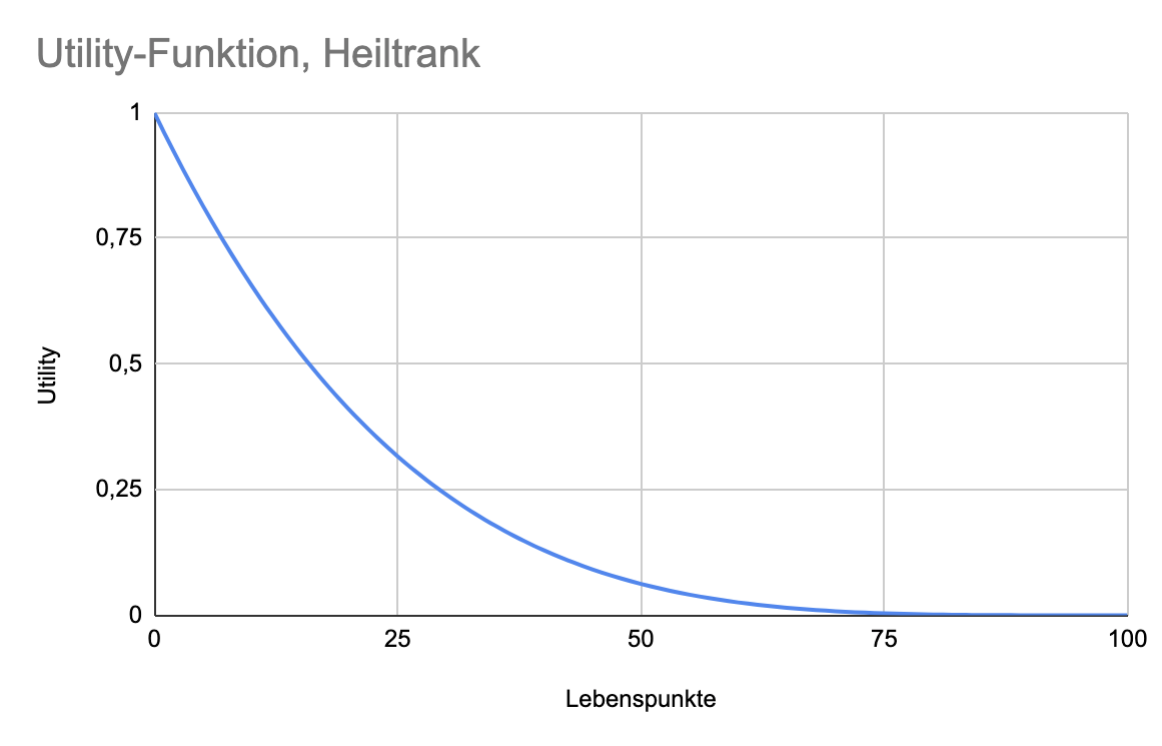
\includegraphics[scale=0.65]{images/chapter_2_int_agents/diagram_utility_1.png}
\caption{Utility-Funktion für Benutzung eines Heiltranks}
\label{fig:utility_1}
\end{figure}

Das Resultat der Verwendung von Utility-Funktionen für das Auslösen bzw. die Auswahl von Aktionen ist die Abbildung eines deutlich dynamischeren Verhaltens als beispielsweise bei der Verwendung einer Finite State Machine.

Eine Variante von Utility-Based Agents sind \Fachbegriff{Needs-Based Agents} \cite{needs_based_agents_1}. Die Utility-Funktionen in dieser Variante basieren auf indiviuellen Motivationen, die menschlichen Bedürfnissen nachempfunden wurden; beispielsweise \aufzaehlung{Hunger}, \aufzaehlung{Durst}, \aufzaehlung{Schlaf} oder \aufzaehlung{Kommunikation} \cite{needs_based_agents_1}. Damit soll ein möglichst menschliches Verhalten simuliert werden.

Mit dem Verfolgen von Bedürfnissen haben Utility-basierte Agenten nicht nur Wurzeln im Design von AI-Systemen, sondern mit der Utility Theory ebenfalls in der Psychologie und Soziologie \cite{utility_gdc}. Durch die beliebige Gestaltung von Bedürfnisfunktionen kann das Verhalten von Agenten verbessert werden. Besonders im Vergleich zu klassischen, statischen Methoden wie Finite State Machines kann daraus ein sinnvolleres, nachvollziehbares Entscheidungsverhalten resultieren. Ein populäres Beispiel für die Verwendung von Utility Based Agents (und in diesem Spezialfall Needs Based Agents) ist das Spiel \Fachbegriff{Die Sims 4} \cite{sims_4}. Das Spiel stellt eine Simulation von menschlichen Bedürfnissen und Beziehungen sowie des menschlichen Alltags dar. Es verwendet Utility-Funktionen für die Repräsentation des internen Zustands der NPCs, um ein annähernd menschliches Verhalten zu erreichen \cite{sims_utility}.










\chapter{Reinforcement Learning}\label{reinforcement_learning}
% hier könnte noch was sinnvolles stehen
% https://github.com/Unity-Technologies/ml-agents/blob/master/docs/Background-Machine-Learning.md
Das vorherige Kapitel \ref{intelligente_agenten} beschäftigt sich mit der Entwicklung intelligenter Agenten zur Erschaffung von künstlicher Intelligenz für virtuelle Entitäten in Videospielen. Der Fokus dieses Kapitels liegt in der Erläuterung von Reinforcement Learning (RiL) als eine alternative Methode. Die Nutzung von Machine Learning stellt den logischen nächsten Schritt zu den bereits vorgestellten Methoden für die Realisierung \textit{lernender} intelligenter Agenten in Videospielen dar. Im Gegensatz zu klassischen Methoden werden hier also Agenten verwendet, die aufgrund ihrer gesammelten Erfahrungen einen Lernprozess durchlaufen. Das Kapitel dient als vorbereitendes Element für die Implementierung von lernenden intelligenten Agenten in einem Dorfsystem als zentrales Thema der vorliegenden Thesis.

Insgesamt wird ein starker Fokus auf \ac{reinforcement_learning} gesetzt. Zunächst wird dafür eine Gegenüberstellung zwischen klassischen Machine Learning-Verfahren und \ac{reinforcement_learning} vorgenommen. Es folgt eine Einordnung der Verfahren in einen übergeordneten Kontext sowie die Beschreibung aktueller Entwicklungen in diesem Bereich. Anschließend werden \acp{markov_problem} als elementare Problemstellung für \ac{reinforcement_learning} diskutiert. Ein Menge konkreter modellfreier und modellbasierter Methoden zur Implementierung des Verfahrens werden ausführlich erläutert. Dafür werden nötige mathematische Grundlagen geschaffen.

Der erste Abschnitt beinhaltet eine Rekapitulation zur grundsätzlichen Funktionsweise von \Fachbegriff{Machine Learning}. Zur Einordnung des Themas in einen übergeordneten Kontext findet anschließend eine Einordnung der klassischen Teilbereiche von Machine Learning und \ac{reinforcement_learning} statt. 




\section{Einordnung}
Maschinelles Lernen beschäftigt sich mit der Entwicklung eines Systems, das aus einer Menge von beliebigen Inputdaten einen gewünschten Output erzeugt. Dabei wird der Versuch unternommen, durch eine Verbesserung des Outputs in Abhängigkeit vom Input einen Lerneffekt zu erzielen. Diese Fähigkeit wird erlangt, indem das System mit relevanten Informationen gespeist wird, aus denen Assoziationen gebildet und Muster erkannt werden können. Dadurch können schlussendlich zukünftige Outputs verbessert werden, ohne dass dieser Vorgang spezifisch definiert wird. Der Lernvorgang passiert nicht durch die Nutzung eines statischen Algorithmus und wird nicht explizit programmiert, sondern wird durch die automatische Anpassung von Werten und Gewichtungen beschrieben, die dem System zugrunde liegen. Häufig werden hierfür neuronale Netze verwendet. Man entscheidet dabei unter anderem zwischen \Fachbegriff{Feedforward}-Netzen und \Fachbegriff{rekurrenten} Netzen. Feedforward-Netze verbinden stets Neuronen aus vorderen Schichten mit Neuronen aus hinteren Schichten. Rekurrente neuronale Netze erlauben auch umgekehrte Verbindungn von vorderen Neuronen zu hinteren Neuronen. So entsteht eine Rückkopplung, die zeitliche Informationen aus zuvor getätigten Entscheidungen mit einbeziehen kann.
Ein System, das einen Input manipuliert, wird also so lange verändert, bis es für jeden Output den gewünschten Input erzeugen kann. Anstatt Beispiele auswendig zu lernen wird ein statistisches Modell erzeugt, das auch unbekannte Daten beurteilen kann. Dieses Modell wir durch eine Menge von Parametern beschrieben, in der Regel handelt es sich dabei um die Gewichtungen der einzelnen Neuronen in einem neuronalen Netz.

Weiterhin sollte geklärt werden, was als Input und als Output für das System genutzt wird. Wir gehen im Folgenden davon aus, dass ein einfaches neuronales Netz verwendet wird, dessen Struktur für die Lösung des folgenden Problems irrelevant ist. Um den Lernvorgang eines Agenten zu ermöglichen, müssen für den Input Werte gewählt werden, die für die Problemstellung relevant sind. Dabei kann es sich um beliebige Informationen aus dem Weltzustand des Spiels handeln. Im Folgenden wird ein Beispiel betrachtet, das indirekt bereits das Vorgehen beim \ac{reinforcement_learning} beschreibt, um das generelle Vorgehen von maschinellem Lernen zu verdeutlichen.

Ein Agent soll lernen, auf einer sich bewegenden Plattform zu balancieren. Für diese Aufgabe gibt es bestimmte relevante Parameter - beispielsweise die Orientierung der Plattform sowie die Orientierung des Agenten. Unter der Annahme, dass keine weiteren äußeren Parameter die Problemstellung beeinflussen, werden diese beiden Vektoren als Inputparameter für das neuronale Netz verwendet. Zusätzlich muss definiert werden, was die Outputparameter des neuronalen Netzes steuern sollen. In diesem simplen Szenario ist es offensichtlich, dass für das Balancieren die Orientierung des Agenten angepasst werden muss.
Nun findet ein Lernvorgang statt, indem durch eine kontinuierliche Änderung der Strategie des Agenten durch die Anpassung seines Modells Beziehungen zwischen Input und Output hergestellt werden können. Der Agent sammelt \Fachbegriff{Erfahrungen}, indem er über einen langen Zeitraum versucht, das Problem zu lösen und währenddessen immer wieder von der Plattform fällt. Einige Entscheidungen führen jedoch dazu, dass der Agent sich länger auf der Plattform halten kann als andere. Es werden Assoziationen zwischen der Orientierung der Plattform und des Agenten sowie dem Erfolg der jeweils gesammelten Erfahrungen gebildet. Das Modell des Agenten bzw. dessen Strategie als Reaktion auf die Inputparameter wird kontinuierlich angepasst, bis der Agent das Balancieren beherrscht.
Man spricht hier vom \textit{Training} eines neuronalen Netzes. Der Trainingsvorgang unterscheidet sich dabei je nach verwendeter Technologie. Es wird weiterhin zwischen \Fachbegriff{Training} und \Fachbegriff{Inference} unterschieden. Die Inference beschreibt die Nutzung eines bereits trainierten Machine Learning-Modells zur Generierung eines Outputs. Dabei werden im Unterschied zum Training keine Gewichtungen mehr angepasst. Das fertige Modell wird nicht verändert, sondern lediglich genutzt.
Generell unterscheidet man zwischen einem überwachten Training mithilfe von bereits bekannten Inputdaten, denen ein bekannter Output zugeordnet wurde oder einem unüberwachten Training, für das derartige Daten nicht vorhanden sind. Weiterhin wird in der vorliegenden Arbeit \ac{reinforcement_learning} als zusätzliche Kategorie angeführt. Im Folgenden werden zunächst unüberwachte und überwachte Methoden näher betrachtetet.

% vorteile, nachteile von ML (geld sparen und besseren content erzeugen)?
% die problematik und den ablauf besser erklären


\subsection{Überwachtes Lernen}\label{supervised_learning}
Das \Fachbegriff{überwachte Lernen} (\Fachbegriff{supervised learning}) basiert auf der Verwendung von Trainingsdaten, die über bestimmte \Fachbegriff{Label} verfügen. Diese Label sind Werte oder Einordnungen in Klassen, die ein bestimmtes Beispiel aus dem Datensatz beschreiben und über die jedes Beispiel des Datensatzes verfügen muss. Beispielsweise könnte es sich um eine Menge von Bildern von Pflanzen handeln, wobei jedes Bild mit dem Namen der Pflanze versehen ist. Diese Klassifizierungen sind bereits vor dem Trainingsvorgang bekannt. Es ist weiterhin genau bekannt, was der Output des Verfahrens ist, nämlich eine Klassifizierung der Beispiele in Klassen von Pflanzen.
Häufig wird diese Methode daher für Klassifizierungsaufgaben verwendet. Dabei müssen allgemeine Muster, Gemeinsamkeiten und Unterschiede zwischen den Beispielen identifiziert werden, sodass das Verfahren aus den gefundenen Merkmalen lernt, Label aus Bildinformationen vorherzusagen. Anders formuliert ist der Input in das neuronale Netz eine Menge von Bildinformationen, der Output ist jeweils ein Label bzw. eine Klasse.
Zusätzlich kann überwachtes Lernen für Regressionen verwendet werden. Es gilt, folgende Frage zu beantworten: \glqq{}Wenn eine Variable $x$ einen bestimmten Wert hat, welchen Wert hat dann $y$?\grqq{}. Ein mögliches Anwendungsszenario wäre ein neuronales Netz, das den Preis einer Wohnung in Hamburg anhand ihrer Lage, Ausstattung und Größe bestimmt.

\subsubsection{Imitation Learning}\label{imitation_learning}
Bei \Fachbegriff{Imitation Learning} (\Fachbegriff{Imitation Learning}) handelt es sich um eine Kombination aus \ac{reinforcement_learning} und überwachtem Lernen, bei der bereits vorhandene Daten verwendet werden, um Sequenzen von zukünftigen Aktionen vorherzusagen \cite{icml_imitation}. Imitation Learning wird häufig in Spielen verwendet um intelligente Agenten zu erschaffen die versuchen, die Aktionen eines Spielers zu imitieren. Man spricht auch von \Fachbegriff{Behavioral Cloning}. Als Trainingsdaten können beispielsweise Aufzeichnungen des Spielverhaltens eines echten Spielers dienen. Sowohl die Beobachtungen aus dem Spielzustand als auch die daraus resultierenden Entscheidungen des Spielers anhand seines Hardwareinputs sind gegeben, um eine Imitation zu ermöglichen. Gegeben sind also sowohl Beobachtungen, als auch die resultierenden Aktionen; nun muss der Zusammenhang zwischen den Beiden gelernt werden. In der Rennspielreihe \Fachbegriff{Forza Motorsport} wurde Imitation Learning erfolgreich eingesetzt, um sogenannte \sogenannt{Drivatars} \cite{forza} zu erstellen. Dabei handelt es sich um Agenten, die genau das Fahrverhalten von spezifischen Spielern imitieren sollen.


\subsection{Unüberwachtes Lernen}\label{unsupervised_learning}
Trainingsdatensätze sind nicht für jedes Machine Learning-Problem gegeben. Tatsächlich ist das Fehlen von gelabelten Daten häufig ein Problem, da das Anfertigen solcher Datenmengen eine lange Zeit in Anspruch nehmen würde oder in bestimmten Szenarien gar nicht möglich ist.
Beim \Fachbegriff{unüberwachten Lernen} bekommt ein neuronales Netz während des Trainingsvorgangs eine Menge von nicht gelabelten Daten ohne spezielle Anweisungen. Anhand von Labeln ist es hier also nicht möglich, bestimmte Merkmale in den Trainingsdaten zu erkennen. Stattdessen werden alternative Ansätze gewählt, zum Beispiel:
\begin{itemize}
    \item \texttt{Clustering}: Bestimmte Charakteristiken oder \Fachbegriff{Features} werden aus den Daten extrahiert. Dabei kann es sich im oben genannten Pflanzenbeispiel um die Größe der Blätter, Farbe der Blüten oder die Form handeln. Die Beispiele werden anhand von Ähnlichkeiten angeordnet, also \sogenannt{geclustered}.
    \item \texttt{Anomaly Detection}: Anomalien in den Features werden erkannt, um \sogenannt{Ausreißer} zu erkennen. Wenn beispielsweise alle Pflanzen im Datensatz gelbe Blüten haben außer Eine, so würde Diese als Anomalie erkannt werden.

Im Gegensatz zum überwachten Lernen ist der Output des Modells unbekannt. Weiß man beispielsweise beim überwachten Lernen genau, dass als Output eine Klassifizierung der Beispiele in eine bestimmte Anzahl von Pflanzenkategorien vorgenommen wird, so muss beim unüberwachten Lernen der Output genau analysiert werden, um ein Verständnis darüber zu erlangen. Es ist weiterhin vorher nicht immer klar, wie viele Kategorien bzw. Cluster gebildet werden und wie die Verteilung der Beispiele aussieht.
Durch das Fehlen von Referenzdaten ist eine Überprüfung der Genauigkeit des Verfahrens beim unüberwachten Lernen oft schwierig.
\end{itemize}


\subsection{Reinforcement Learning}\label{reinforcement_learning_intro}
Der Begriff \Fachbegriff{Reinforcement Learning} beschreibt ein Verfahren, in dem ein Agent eigenständig lernt, sinnvolle Entscheidungen zu treffen, indem aus einer Menge von Aktionen diejenigen ausgewählt werden, die eine Belohnungsfunktion maximieren \cite{ai_for_game_devs} \cite{reinforcement_introduction_book} \cite{dammann_reinforcement} \cite{alzantot_0} \cite{intel_ai_demystifying}. Zur Anwendung kommt es neben Videospielen ebenfalls in der Robotik oder in der Medizin. Der grundsätzliche Ablauf von \ac{reinforcement_learning} wird in Abbildung \ref{fig:reinforcement_flow} dargestellt.

\begin{figure}[H]
\centering
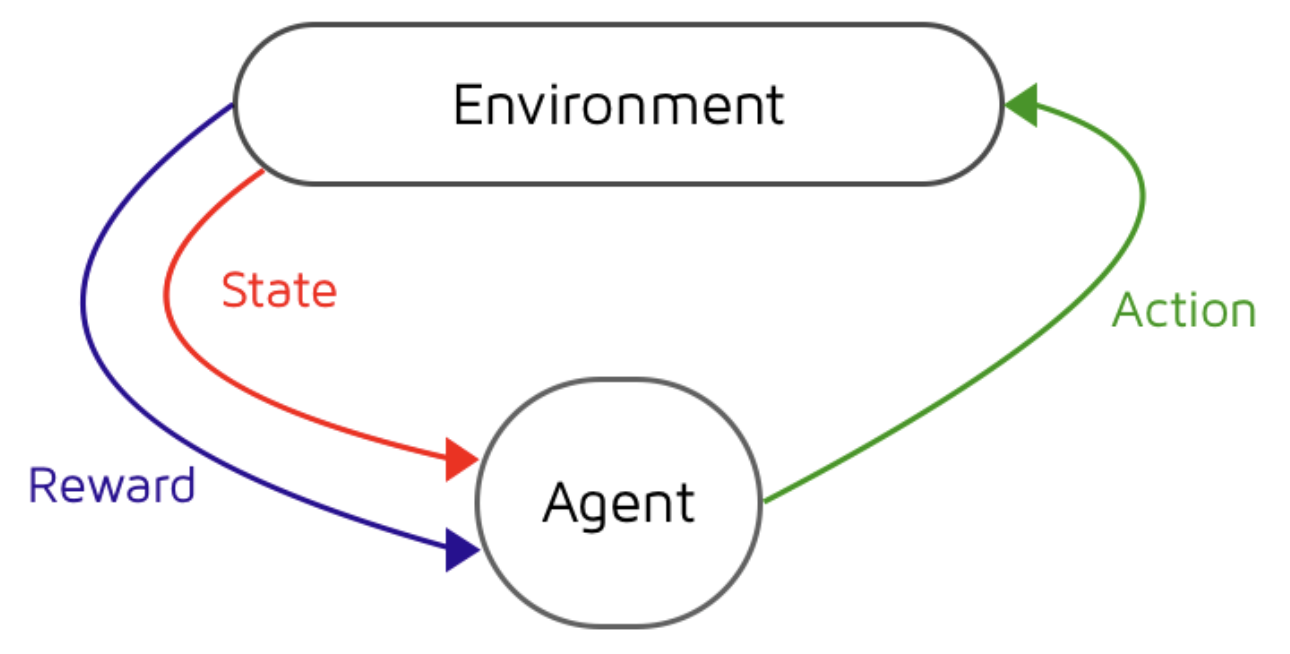
\includegraphics[scale=0.45]{images/reinforcement_flow.png}
\caption{Grundsätzlicher Ablauf von \ac{reinforcement_learning} \cite{intel_reinforcement_openai_gym_blog}}
\label{fig:reinforcement_flow}
\end{figure}

Die Ausführung einer Aktion versetzen den Agenten in einen neuen Zustand und resultiert in einer Belohnung (\Fachbegriff{Reward}) oder einer Bestrafung (\Fachbegriff{Punishment}). Es handelt sich um einen skalaren Wert, der beschreibt, wie gut der Agent sich verhalten hat. Der Zustand des Agenten wird durch Beobachtungen (\Fachbegriff{Observations}) aus seiner Umgebung (\Fachbegriff{Environment}) beschrieben. Der Agent soll aus seinen Erfahrungen lernen, indem er die besten Aktionen wählt, die die zukünftige Summe seiner Belohnungen maximieren. Der Lernvorgang erfolgt dabei durch die kontinuierliche Änderung seiner Entscheidungsstragie in Abhängigkeit von seinem Zustand, indem beispielsweise Gewichtungen in einem zugrunde liegenden neuronalen Netz angepasst werden. Dabei wird der Versuch unternommen, die Belohnungsfunktion zu maximieren, indem die Beziehungen zwischen Beobachtungen und gewählten Aktionen, sowie den jeweils resultierenden Belohnungen modelliert werden. Für die Suche der besten Entscheidung werden zusätzlich zukünftige Belohnungen berechnet und mit einbezogen (siehe \Fachbegriff{Markov Decision Problems} in Abschnitt \ref{markov_decision_problems}). Generell muss nicht explizit ein klares Ziel definiert werden, stattdessen führt das eigenständige Lernen dazu, dass sich das optimale Verhalten eines Agenten automatisiert ergibt.


Eine Kategorisierung von \ac{reinforcement_learning} in \Fachbegriff{überwachtes Lernen} oder {unüberwachtes Lernen} (siehe Abschnitte \ref{supervised_learning} und \ref{unsupervised_learning}) ist schwierig. Im Gegensatz zum unüberwachten Lernen können den möglichen Aktionen konkrete Werte zugewiesen werden, die das Verhalten des Agenten bewerten. Anstelle des Aufspürens von Anomalien oder Clustern wird also versucht, dem Verhalten des Agenten einen Wert bzw. ein \textit{Label} zuzuweisen. Im Unterschied zum überwachten Lernen werden hier allerdings keine gelabelten Trainingsdatensätze verwendet, sondern eine Menge von Belohnungswerten die sich erst zur Zeit des Trainingsvorgangs ergeben. Bei der Entscheidungsfindung sind beim Reinforcement Learning zudem nicht nur einzelne Vorhersagen relevant, sondern ganze Sequenzen. Man kann also weder von überwachtem, noch von unüberwachtem Lernen sprechen. \ac{reinforcement_learning} wird daher als eine zusätzliche Kategorie betrachtet, die sich von den genannten klassischen Verfahren abgrenzt und eine Art Hybrid-Verfahren darstellt.

Für die Entwicklung intelligenter Agenten ist unüberwachtes Lernen im klassischen Sinne nicht geeignet, da dort mit der Extrahierung markanter Features und Zusammenhänge in Datensätzen ein gänzlich anderes Ziel verfolgt wird. Wegen fehlender gelabelter Datensätze eignet sich auch überwachtes Lernen nicht. Man stelle sich ein Szenario vor, in dem ein Agent das Schachspielen lernen soll: Für eine große Menge von denkbaren Situationen würden dann Daten mit dem jeweiligen Label für den korrekten auszuwählenden Zug benötigt. Diese große Datenmenge müsste mühselig angefertigt bzw. gesammelt werden. Im deterministischen Falle von Schach wäre das Sammeln dieser Daten beispielsweise durch die Aufzeichnung von Spielen in einer Schachapp möglich. Diese Möglichkeit ist jedoch nicht mehr gegeben, sobald das Zielverhalten des Agenten unbekannt ist oder die Umgebung nicht-deterministische Strukturen aufweist.
\ac{reinforcement_learning} bietet hingegen ein leicht zu handhabendes Framework, in dem Probleme auf eine simple Art und Weise beschrieben werden können. In der Theorie müssen hier lediglich gute Züge positiv und schlechte Züge negativ bewertet werden, sodass der Agent aus den Belohnungen in Kombination mit seinen Beobachtungen Schlüsse ziehen kann. Weiterhin fällt die Notwendigkeit von großen (gelabelten) Datensätzen weg.
Aktuelle Projekte (siehe Kapitel \ref{aktuelle_entwicklungen_rl}) zeigen dabei vielversprechende Ergebnisse und beweisen sowohl die Skalierbarkeit als auch das hohe Lernpotential von \ac{reinforcement_learning}-basierten Algorithmen. Mit Projekten wie \Fachbegriff{OpenAI Gym} \cite{openai_gym} und \Fachbegriff{ML-Agents} \cite{ml-agents_paper} (siehe Abschnitt \ref{ml_unity}) stehen darüber hinaus umfangreiche Umgebungen und Bibliotheken für die Einbindung in Spiele bereit. Weiterhin finden sich keine vergleichbaren Ansätze in der Fachliteratur, die auf \ac{reinforcement_learning} zur Definition des Verhaltens von \acp{npc} setzen, wodurch ein Gegenpol zu klassischen Verfahren gesetzt und eine neuartige Methode getestet werden kann.

\ac{reinforcement_learning} bietet aus den genannten Gründen den sinnvollsten und möglichweise einzigen realistischen Lösungsansatz für das gebotene Problem und wird daher in der vorliegenden Arbeit verwendet.




















\section{Markov Decision Problems}\label{markov_decision_problems}
Dieses Kapitel beschäftigt sich mit der Erläuterung von \acp{markov_problem} als Grundlage für das \Fachbegriff{Reinforcement Learning}, welches die Lösung von \Fachbegriff{Markov-Problemen} anstrebt. Daher bilden sie eine wichtige Basis für das folgende Kapitel. 
Bei Markov-Problemen (bzw. \Fachbegriff{Markov-Entscheidungsproblemen}) handelt es sich um ein Modell für Entscheidungsprobleme, bei denen ein Agent versucht, eine Belohnungsfunktion zu maximieren \cite{ai_for_game_devs} \cite{reinforcement_introduction_book} \cite{deep_reinforcement_paper} \cite{art_int_mod_app} \cite{dammann_reinforcement} \cite{alzantot} \cite{mohammad_markov}. Zu jeder Entscheidung befindet sich der Agent in einem bestimmten Zustand und verfügt über eine Menge von Aktionen, aus denen er wählen kann. Durch die Ausführung von Aktionen bewirkt der Agent Übergänge in andere Zustände. Es muss einen oder mehrere Endzustände geben, die die Ausführung abbrechen, sobald sie erreicht werden. Die Wahrscheinlichkeit für die Auswahl einer Aktion liegt jeweils bei einem Wert von $p < 1$.
Wenn ein Agent stets die beste Entscheidung trifft, dann spricht man von einer optimalen \Fachbegriff{Policy} für die Lösung des Problems. Eine Policy ist also eine Strategie des Agenten in Abhängigkeit von seinem Zustand, welcher durch Beobachtungen aus seiner Umgebung festgelegt wird. Diese werden auch \Fachbegriff{Observations} genannt. Die Policy kann weiterhin definiert werden als eine Funktion vom Zustand eines Agenten zu einer Wahrscheinlichkeitsverteilung über die möglichen Aktionen \cite{openai_five_paper}.

\subsection{Beispiel}
Im folgenden Beispiel wird ein Roboter betrachtet \cite{markov_robot_example}, der sich jeweils um ein Feld in vier Richtungen bewegen kann. Wenn dieser die Wände des in Abbildung \ref{fig:markov_problem_1} sichtbaren Spielfelds berührt, dreht er automatisch um und bewegt sich in die gegenüberliegende Richtung. Nur die weißen Felder sind passierbar. Felder, die mit einer Zahl versehen sind, geben Belohnungen oder Bestrafungen. Hier wird ein skalarer Wert $+1$ oder $-1$ genutzt. Das Feld mit einer Bestrafung heißt \Fachbegriff{Bestrafungsfeld}. Weitere Felder resultieren jeweils in einer Bestrafung von $-0.04$. Das Ziel ist es, den besten Weg zum Ziel (dem Feld mit der \textit{+1}) mit der höchsten Belohnung für den Roboter zu finden.

\begin{figure}[H]
\centering
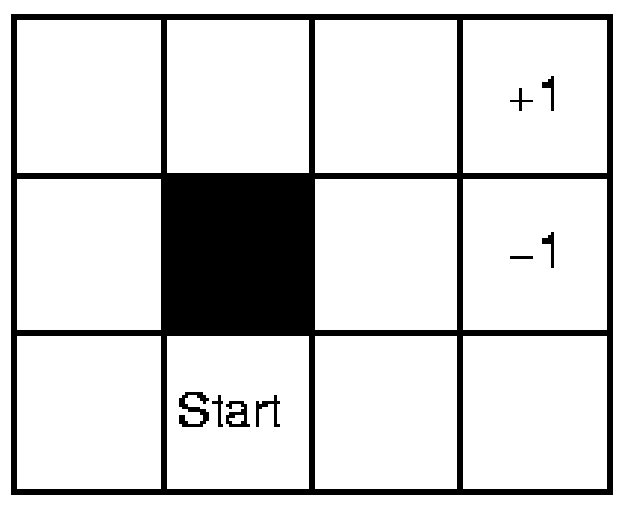
\includegraphics[scale=0.4]{images/markov/markov_problem_1.png}
\caption{Deterministisches MDP \cite{markov_robot_example}}
\label{fig:markov_problem_1}
\end{figure}

Betrachtet wird nun ein deterministischer Ansatz. Hier gehen wir davon aus, dass der Roboter die Aktionen, die er auswählt, immer korrekt ausführt. Als bester Weg ergibt sich dabei mathematisch der kürzeste Weg, wie in Abbildung \ref{fig:markov_problem_2} zu sehen. Da das Szenario leicht in einen Graphen mit Kosten transformiert werden kann, ist offensichtlich, dass Suchverfahren wie A* verwendet werden können, um den optimalen Pfad zu finden.

\begin{figure}[H]
\centering
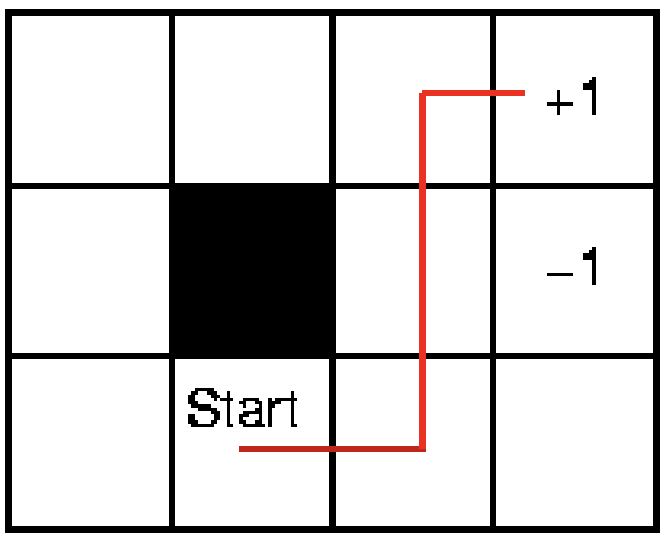
\includegraphics[scale=0.39]{images/markov/markov_problem_2.png}
\caption{Lösung des deterministischen MDP \cite{markov_robot_example}}
\label{fig:markov_problem_2}
\end{figure}

Nun wird ein nichtdeterministischer bzw. stochastischer Ansatz gewählt. Bei solchen Problemen spricht man von einem \ac{pomdp}. Die Zustandsübergänge bekommen dann einen stochastischen Wert zugewiesen. Das bedeutet, dass der Roboter Aktionen nun mit einer gewissen Wahrscheinlichkeit korrekt oder inkorrekt ausführen kann. Die Umgebung des Agenten ist also nichtdeterministisch.

Die Wahrscheinlichkeiten für das Roboter-Beispiel sind in Abbildung \ref{fig:markov_problem_3} erkennbar. Der Agent hat in seiner Laufrichtung eine Chance von $p = 0,8$ und zu den Seiten hin jeweils eine Wahrscheinlichkeit von $p = 0,1$. Das bedeutet, dass der Agent nur in 80\% der Fälle die gewünschte Aktion und in 20\% der Fälle die falsche Aktionen ausführt.

\begin{figure}[H]
\centering
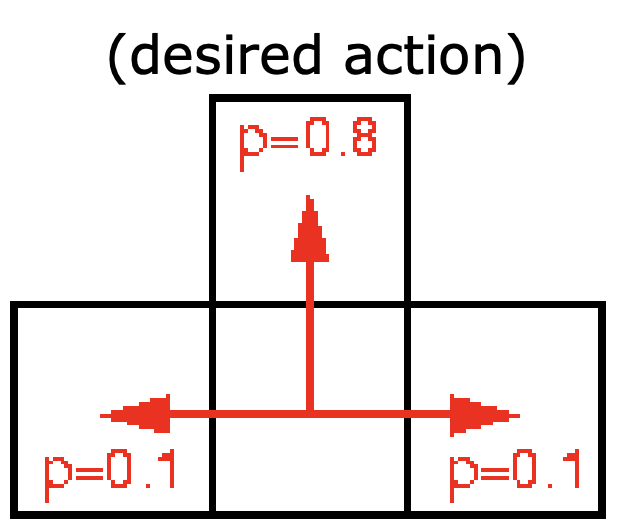
\includegraphics[scale=0.34]{images/markov/markov_problem_3.png}
\caption{Nichtdeterministisches MDP \cite{markov_robot_example}}
\label{fig:markov_problem_3}
\end{figure}

\begin{figure}[H]
\centering
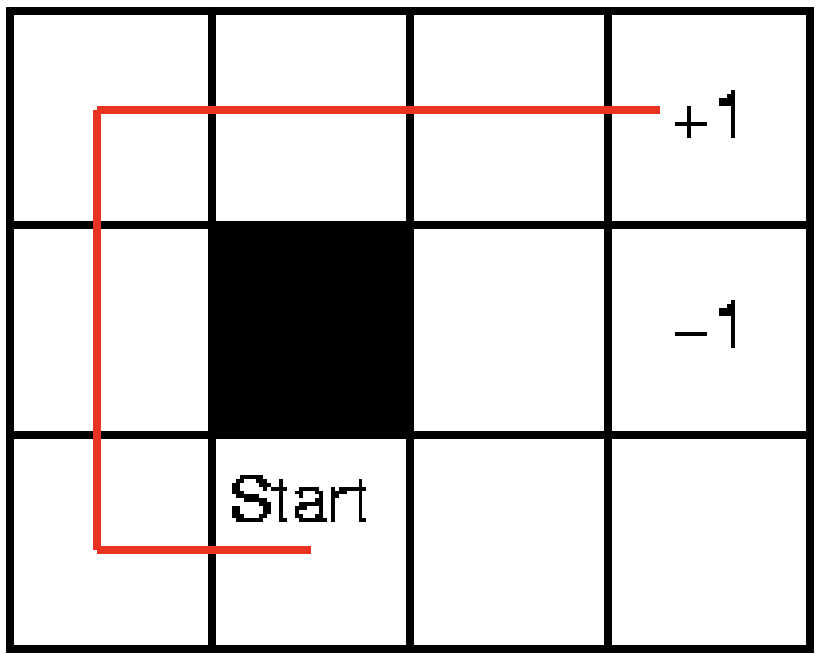
\includegraphics[scale=0.32]{images/markov/markov_problem_4.png}
\caption{Lösung des nichtdeterministischen MDP \cite{markov_robot_example}}
\label{fig:markov_problem_4}
\end{figure}

Abbildung \ref{fig:markov_problem_4} zeigt den resultierenden besten Weg. Anstatt den kürzesten Weg zu wählen wird nun ein Weg gewählt, bei dem die Wahrscheinlichkeit geringer ist, durch eine falsch ausgeführte Aktion versehentlich das Bestrafungsfeld zu betreten. Statistisch gesehen ergibt sich daraus die höchste Belohnung für den Agenten. In diesem Fall kann das Problem also nicht ohne Weiteres durch einen Suchalgorithmus gelöst werden, da es nichtdeterministisch ist.



\subsection{Formale Beschreibung}
Nachdem im vorherigen Kapitel zum Verständnis je ein Beispiel für ein deterministisches \ac{markov_problem} und ein nichtdeterministisches \ac{markov_problem} geliefert wurde, folgt in diesem Abschnitt eine formale Beschreibung von Markov-Problemen.


Sei $N$ ein Agent in einer Umgebung $\epsilon$ mit einer Anzahl diskreter Zeitschritte $t$. Die Umgebung kann beispielsweise durch eine virtuelle Welt in einem Spiel dargestellt werden. $N$ verfügt über endlich viele Zuständen $s_t$ aus der Menge aller möglichen Zustände $\mathbb{S}$ mit einer jeweils dazugehörigen Aktion $a_t$. Die jeweils nächsten Zustände heißen $s_t+1$ und $a_t+1$. Zu jedem Zeitschritt $t$ wählt $N$ durch $\pi$ eine neue Aktion $a_t$ aus einer endlichen Menge von Aktionen $\mathbb{A}$. Der Agent $N$ erhält nach $a_t$ einen neuen Zustand $s_t+1$ und eine Belohnung $r_t$. Dieser Prozess wiederholt sich, bis ein  Terminalzustand $s_t$ erreicht wurde.

$N$ verfügt über eine Policy $\pi$. Diese wurde bereits definiert als eine Funktion, die den aktuellen Zustand $s_t$ aus $\mathbb{S}$ nimmt und eine Aktion $a_t$ aus $\mathbb{A}$ zurückgibt. Formal wird $\pi$ also wie folgt beschrieben:
$$ \pi(s_t) : \mathbb{S} \rightarrow \mathbb{A} $$

Aus den einzelnen Belohnungen ergibt sich dann eine akkumulierte Gesamtbelohnung $R_t$, wobei gilt:
$$   R_t   =   \sum_{k=0}^{\infty} {\gamma^k * r_{t+k}}   $$

Die Summe von $0$ bis $\infty$ wird gebildet, weil davon ausgegangen wird, dass es kein Zeit- bzw. Zeitschrittlimit gibt. In der oben sichtbaren Definition beschreibt $\gamma$ den sogenannten \Fachbegriff{Discount-Faktor}. Er wird wie folgt definiert:
$$ \gamma \in \interval[open left]{0}{1} $$

Nach jeder ausgeführten Aktion werden alle Belohnungen, die der Agent theoretisch noch erreichen kann, mit $\gamma$ multipliziert. Dies führt dazu, dass weiter in der Zukunft liegende Belohnungen eine geringere Gewichtung bekommen. Eine weit entfernte hohe Belohnung kann durch die Gewichtung des Discount-Faktors eine deutlich kleinere tatsächliche Belohnung darstellen und damit für den Agenten \sogenannt{uninteressant} werden. Der optimale Lösungsweg wird durch einen Discount-Faktor $\gamma < 1$ so  verändert, dass der Agent im Allgemeinen kürzere Wege bevorzugt. Zu kleine Werte führen dazu, dass der Agent keine langfristigen Belohnungen berücksichtigen kann und kurzsichtige Entscheidungen trifft.

Das Ziel des Agenten ist also die Maximierung der gesamten zukünftigen Belohnung, also der Gesamtbelohnung $R_t$ für jeden Zustand $s_t$. Die potentielle Belohnung wird durch die gewichtete Summe der erwarteten Belohnungswerte für alle zukünftigen Aktionen gebildet, wobei alle möglichen Aktionen in Betracht gezogen werden. Dadurch wird effektiv die aktuell auszuwählende Aktion durch zukünftige Belohnungen beeinflusst.

Es wurde ein Beispiel für Markov-Probleme demonstriert und eine formale Beschreibung aufgestellt. Der nächste Schritt besteht nun in der Lösung von Markov-Problemen. Als weitere Voraussetzung wird im Folgenden kurz die \Fachbegriff{Markov-Eigenschaft} erläutert.



\subsection{Markov-Eigenschaft}
Es wird ein Szenario betrachtet, in dem ein Agent die Zustände $A$, $B$, $C$ und $D$ annehmen kann \cite{markov_property_example}. Die Wahrscheinlichkeit für das sequentielle Auftreten der genannten Zustände hintereinander kann wie folgt faktorisiert werden:

$$ p(A,B,C,D) = p(A) p(B|A) p(C|A,B) p(D|A,B,C)   \;\; $$
$$ \;\;\;\;\;\;\;\;\;\;\;\;\;\;\;\;\;\;\;\;\;\;\;\;\; = p(B) p(A|B) p(C|A,B) p(D|A,B,C)   \;\; ... $$
$$ \;\;\;\;\;\;\;\;\;\;\;\;\;\;\;\;\;\;\;\;\;\;\;\;\; = p(C) p(A|C) p(B|A,C) p(D|A,B,C)   \;\; ... $$
$$ \;\; ... $$

Die \Fachbegriff{Markov-Eigenschaft} gilt, wenn es eine ausgezeichnete (z.B zeitliche) Anordnung gibt, für die sich die Darstellung wie folgt vereinfachen lässt \cite{markov_property_example}:

$$ p(A,B,C,D)  = p(A) p(B|A) p(C|B) p(D|C) $$

Das bedeutet, dass die Wahrscheinlichkeit für den nächsten Zustand nur unmittelbar von dem vorherigen Zustand abhängt. Die Wahrscheinlichkeit für $C$ hängt also nur vom vorherigen $B$ und nicht von dem ursprünglichen $A$ ab.
\section{Modellfreie und modellbasierte Verfahren}\label{reinforcement_learning_basics}
Konkret werden beim Reinforcement Learning Markov-Entscheidungsprobleme gelöst. Es gibt also, wie in Kapitel \ref{markov_decision_problems} definiert, einen Agenten mit einer Menge von Zuständen, einer Menge von Aktionen und einer Policy, die optimiert werden soll, indem Belohnungen von Aktionen in Abhängigkeit von Beboachtungen bzw. \Fachbegriff{Observations} in Betracht gezogen werden. 

Man unterscheidet zwischen \Fachbegriff{modellbasierten} und \Fachbegriff{modellfreien} Ansätzen (\Fachbegriff{model-based} und \Fachbegriff{model-free}) \cite{berkely_modelfree_modelbased_rl}. Dabei geht es nicht um die Verwendung eines Modells im Sinne von einer Belegung/Gewichtung der Neuronen eines neuronalen Netzes. Dieser Begriff wird häufig beim überwachten Lernen verwendet, beschreibt aber nicht die selbe Sache.

Beim modellbasierten Lernen verfügt der Agent über Informationen zu seinen möglichen Zuständen und Aktionen. Ihm sind sowohl alle möglichen Zuständsübergänge als auch die nötigen Aktionen bekannt, die diese auslösen. Er verfügt also über ein Modell, das seine Umgebung repräsentiert. Dies gibt ihm die Möglichkeit, vorauszuplanen und zukünftige Belohnungen direkt zu berechnen.

Man spricht vom modellfreien Lernen, wenn ein Agent lediglich aus gesammelten Erfahrungen Rückschlüsse über seine Zustände und Aktionen treffen kann. Für das Treffen von Entscheidungen verlassen sich derartige Verfahren auf vergangene Beispiele aus ihrer Umgebung, ohne direkte Vorhersagen über den nächsten Zustand zu treffen. Der Agent verwendet also eine Art \sogenannt{Trial-And-Error}-Verfahren für die Berechnung einer möglichst guten Policy.



\subsection{Modellbasierte Verfahren}
Im Folgenden werden einige relevante modellbasierte Verfahren konkret vorgestellt. Als erstes werden dafür weitere nötige Grundlagen geschaffen, indem zugrunde liegende Sachverhalte wie die \Fachbegriff{Bellman}-Gleichung erläutert werden.


\subsubsection{Grundlagen modellbasierter Verfahren}
Das im Kapitel \ref{markov_decision_problems} vorgestellte Beispiel eignet sich gut für modellbasierte Verfahren. Der Agent kennt das \ac{markov_problem}-Modell der Welt mit Zustandsübergängen, Aktionen und Wahrscheinlichkeitsverteilungen.

Zunächst wird eine sogenannte \Fachbegriff{Value Function} aufgestellt, die beschreibt, wie gut ein Zustand für einen Agenten ist. Sie entspricht der erwarteten Belohnung ausgehend von einem Startzustand. Die Funktion hängt von der Policy $\pi$ des Agenten ab \cite{alzantot} \cite{intro_to_ml_book}.
$$    V^{\pi}(s)  =   \mathbb{E} \; [  \:  \sum_{k=0}^{\infty} {\gamma^k * r_{t+k}} ]   \;\;\;   \forall{s} 	\in{ \mathbb{S} }     $$

Das Symbol $\mathbb{E}$ steht dabei für einen Erwartungswert. Die Value Function für einen bestimmten Zustand und eine bestimmte Policy berechnet also für alle Zustände $s$ aus $\mathbb{S}$ die erwartete Gesamtbelohnung, welche sich aus den einzelnen Belohnungen der einzelnen Zustände bzw. Aktionen auf dem Weg bis zum Zielzustand befinden.

Es existiert eine Optimale Value Function $V^*$, die von allen Funktionen den höchsten Reward liefert.
$$   V^*(s)   =   \mathmax_{\pi} \; V^{\pi}(s)    \;\;\;   \forall{s} 	\in{ \mathbb{S} }     $$


Weiterhin existiert eine optimale Policy ${\pi}^*$, welche in der optimale Value Function resultiert.
$$   {\pi}^*   =  \argmax_{\pi}  \; V^{\pi}(s)    \;\;\;   \forall{s} 	\in{ \mathbb{S} }     $$



Weiterhin wichtig für sowohl modellbasierte als auch modellfreie Verfahren sind sogenannte \Fachbegriff{Q-Functions}. Diese nutzen einen Zustand $s$ und eine Aktion $a$. Dabei wird ein Mapping von Zuständen zu möglichen Aktionen verwendet. Eine Q-Function gibt einen reellen Wert zurück, der die zu erwartende Belohnung widerspiegelt, wenn im Zustand $s$ die Aktion $a$ ausgeführt wird.
$$  \mathcal{Q}  \;\,  :  \;\,  \mathbb{S} \, \times   \, \mathbb{A}  \;  \rightarrow  \;  \mathbb{R}  $$

Die optimale Q-Funktion lautet $Q^*(s,a)$. Ein Agent startet dann in Zustand $s$ und führt bis zum Terminalzustand nur optimale Aktionen aus. Sie gibt Angaben darüber, wie gut ein Zustand für einen Agenten ist, wie die optimale Value Function $V^*$. Da $V^*$ die maximal zu erwartende Belohnung beim Start in Zustand $s$ ist, so wäre das Q-Äquivalent das Maximum von $Q^*(s,a)$ über alle möglichen Aktionen. Also gilt:

$$   V^*(s)   \;\; = \;\;   \mathmax_a Q^* (s,a)  \;\;\;   \forall{s} 	\in{ \mathbb{S} }   $$

$$   {\pi}^*   \;\; = \;\;   \argmax_a Q^* (s,a)  \;\;\;   \forall{s} 	\in{ \mathbb{S} }   $$



\paragraph{Bellman-Gleichung}
Die beiden modellbehafteten Verfahren \Fachbegriff{Value Iteration und Policy Iteration} und weitere Ansätze nutzen die \Fachbegriff{Bellman-Gleichung} \cite{bellman}. Die Gleichung stellt ein Optimierungsverfahren dar.
Die Q-Funktion $Q^*(s,a)$ entspricht laut Bellman der Summe der unmittelbaren Belohnungen der Aktion $a$ aus Zustand $s$ heraus und der mit dem Discountfaktor verrechneten zukünftigen Belohnung nach der Zustandsänderung in einen neuen Zustand $s'$ \cite{alzantot} \cite{intro_to_ml_book} \cite{unity_blog_reinforcement_q} \cite{alzantot}.

$$   Q^* (s,a) = R(s,a) + \gamma  \:  \mathbb{E}_{s'}   \:   [V^*(s')]    $$

$$   Q^* (s,a) = R(s,a) + \gamma  \:  \sum_{s' \in{\mathbb{S}} } p'(s|s,a) \; V^*(s')    $$

$$   V^*(s)  \: = \:  \mathmax_a  \;  \left[   R(s,a) + \gamma  \:  \sum_{s' \in{\mathbb{S}} } p'(s|s,a) \; V^*(s')   \, \right] $$





\subsubsection{Value Iteration}
Value Iteration nutzt die Bellman-Gleichung zur iterativen Berechnung der optimalen Value Function $V(s)$. Es garantiert immer nach $n$ Schritten eine Konvergenz zur optimalen Value Function. Der Ablauf von Value Iteration wird anhand des folgenden Pseudocodes verdeutlicht \cite{intro_to_ml_book}:

% Explanation: https://www.quora.com/What-is-an-intuitive-explanation-of-value-iteration-in-reinforcement-learning-RL

\smallskip
\begin{algorithm}[H]
\SetAlgoLined
\KwResult{Optimal Value Function}
\smallskip
Initialize $V(s)$ to arbitrary values\;
\While{$V(s)$ has not converged}{
    \For{all $s \in{ \mathbb{S} } $}{
        \For{all $a \in{ \mathbb{A} } $}{
            $ Q(s,a) \leftarrow  \mathbb{E}[r|s,a] + \gamma \, \sum_{s' \in{\mathbb{S}} \: } p'(s|s,a) \; V^*(s')  $
        }
        $ V(s)   \leftarrow   \mathmax_a Q(s,a)   $
    }
}
\caption{Value Iteration}
\end{algorithm}
\smallskip
\smallskip

Bei diesem Vorgehen wird eine relativ willkürliche Endbedingung festgelegt. Es sollte ein sinnvoller Wert für die erreichte Konvergenz der Value Function als Abbruchbedingung gefunden werden.

Die Funktion beinhaltet einen rekursiven Abstieg. $V(s)$ wird so lange mit dem jeweils nächsten Zustand aufgerufen, bis das Ende erreicht wird, wobei für jeden Zwischenzustand alle möglichen Aktionen ausgewertet und jeweils die mit der maximalen Belohnung $R$ gewählt wird.
Dies wird für jeden möglichen Startzustand aus $\mathbb{S}$ und jede mögliche Aktion wiederholt.


\subsubsection{Policy Iteration}
Das Vorgehen bei \Fachbegriff{Policy Iteration} verfolgt den Ansatz, statt der optimalen Value Function die optimale Policy zu finden. Bei jedem Schritt wird hier also die Policy angepasst, bis diese konvergiert. Ebenso wie bei Value Iteration wird hier eine Konvergenz für ein optimales Ergebnis nach $n$ Schritten garantiert.
Im folgenden Pseudocode wird die Funktionsweise der Policy Iteration gezeigt \cite{intro_to_ml_book}:

\smallskip
\begin{algorithm}[H]
\SetAlgoLined
\KwResult{Optimal Policy}
\smallskip
Initialize a policy $\pi$\ arbitrarily\;
\While{$\pi$ != ${\pi}'$}{
    $ \pi \leftarrow {\pi}' $   \;
    Compute Value Functions for $\pi$ by solving linear equations\;
        $ \;\;\;\;\;\;   V^{\pi}(s) = \mathbb{E} [r|s, \pi(s)]  +  \gamma \sum_{s'in \mathbb{S}}  \;  P(s'|s,\pi(s)) V^{\pi}(s')   $   \;
    Improve the policy at each state\;
        $ \;\;\;\;\;\;    {\pi}'(s)  \leftarrow  \argmax_a \left(  \mathbb{E}[r|s,a]   +  \gamma \, \sum_{s' \in{\mathbb{S}} \: } P(s'|s,a) \; V^{\pi}(s')  \right)  $  \;
}
\caption{Policy Iteration}
\end{algorithm}
\smallskip
\smallskip

Das Verfahren läuft so lange, wie die jeweils neu berechnete Policy eine Änderung erfährt. Sobald ${\pi}'$ gleich $\pi$ gilt, terminiert der Algorithmus.
In jedem Schritt werden zunächst die Value Functions für die aktuelle Policy $\pi$ berechnet. Diese bestehen jeweils aus dem erwarteten Reward, der sich aus dem aktuellen State mit der aktuellen Policy ergibt sowie der mit $\gamma$ verrechneten Summe aller nächsten Zustände $s'$ je nach der durch die Policy bestimmten Wahrscheinlichkeit. Dabei gibt es erneut einen rekursiven Abstieg durch das Aufrufen von $V^{\pi}(s')$ mit allen weiteren Zuständen $s'$ bis hin zum Erreichen des Endzustands.

Nach der Berechnung aller Value Functions für die aktuelle Policy $\pi$ wird die neue Policy ${\pi}'$ berechnet. Für jeden möglichen Zustand $s$ werden mittels der berechneten Value Functions alle möglichen Wege zum Ziel berechnet und jeweils der mit der höchsten Belohnung gewählt.


\subsection{Modellfreie Verfahren}
In diesem Abschnitt werden modellfreie Verfahren als Gegensatz zu modellbasierten Verfahren behandelt. Es werden einige der konkrete Beispiele genannt. Dabei sollen die jeweils erfolgreichsten Verfahren hinsichtlich ihrer Funktionsweise und mathematischen Abläufen betrachtet werden. Ein besonderer Fokus wird dabei auf Gradientenverfahren gesetzt.
Im Folgenden werden konkrete modellfreie Verfahren vorgestellt.



\subsubsection{Q-Learning}\label{q-learning}
Value Iteration und Policy Iteration garantieren stets ein Ergebnis mit einer optimalen Lösung für ein Problem. Dies ist nur möglich, weil es sich um modellbehaftete Vorgehen handelt, bei denen alle Zustandsübergänge und deren Effekte bekannt sind.

Beim \Fachbegriff{Q-Learning} ist dies nicht der Fall. Q-Learning gehört zu der Kategorie des \Fachbegriff{Temporal Difference Learning}. Beim Temporal Difference Learning passt der Agent nach jeder ausgeführten Aktion seine Policy an, indem die Erwartungen für jede mögliche Aktion für den aktuellen Zustand des Agenten geschätzt werden. Der Unterschied zu Policy Iteration ist, dass es sich um ein modellfreies Verfahren handelt. Dabei werden beim Lernvorgang keine vorausschauenden Aktionen getätigt - der Agent lernt lediglich aus seinen eigenen Erfahrungen. Anstelle der mathematischen Erkundung aller möglichen Wege bis zum Zielzustand werden also viele Samples aus der Erfahrung des Agenten gemacht, um statistisch festzuhalten, welche Aktion in welchem Zustand die sinnvollste ist.

\subsubsection{Q-Tables}
Beim Q-Learning werden Tupel aus Zuständen, Aktionen und Belohnungen gebildet. Diese Tupel füllen dann eine Lookup-Table aus Wertepaaren. Jede Kombination aus für den Agenten nötigen Beobachtungen $n$ ergeben dabei einen neuen State. Die gefüllte Tabelle enthällt pro Zustand Werte für jede mögliche Aktion, die Auskunft darüber geben, wie gut die Aktion mit diesem Zustand ist. Typischerweise wird diese \Fachbegriff{Q-Table} mit Zufallswerten gefüllt. Unter Anwendung des Temporal Difference Learnings werden die optimalen Zustand-Aktion-Tupel approximiert.
Wenn in einem Zustand $s$ eine Aktion $a$ mit einer registrierten Belohnung $r(s,a)$ ausgeführt wird, so funktioniert die Berechnung des neuen Tupels $Q(s,a)$ wie folgt:

$$ Q(s,a) = (1 - \alpha) \: Q(s,a) + \alpha \; Q_{obs} (s,a) $$
$$ Q_{obs} (s,a) = r(s,a) + \gamma \: \mathmax_{a'} \: Q(s',a')  $$

Bei $\alpha$ handelt es sich um die Lernrate. Der neue Wert von $Q(s,a)$ ergibt sich aus der Addition des alten Werts mit dem neuen observierten Wert $Q_{obs}$, jeweils verrechnet mit $\alpha$. $Q_{obs}$ wird aus dem registrierten Belohnungswert und dem maximalen Q-Wert für den neuen Zustand $s'$ errechnet.

Abhängig von der Anzahl der relevanten Variablen und damit den Zuständen ergeben sich daraus unter Umständen sehr große Lookup-Tabellen. Man stelle sich ein Spielfeld von vier mal vier Feldern vor. Jedes Feld kann entweder ein Hindernis, ein Ziel oder nichts beinhalten. Jedes der ingesamt 16 Felder kann also drei verschiedene Feldzustände annehmen. Selbst aus diesem minimalistischen Szenario ergeben sich bereits $n_s = 3^{16} \approx 43 $ Millionen maximal mögliche Zustände. Diese Zahl müsste zusätzlich noch mit der Anzahl der Aktionen multipliziert werden, um die Anzahl der Q-Werte zu erhalten. Beim Q-Learning muss der Agent in der Lage sein, über möglichst alle möglichen Zustände zu abstrahieren, indem er aus seinen gesammelten Erfahrungen lernen kann, um die Q-Tabelle sinnvoll zu füllen. Das setzt auch voraus, dass genügend Erfahrungen gesammelt werden. Ab einer zu hohen Menge von Zuständen ist dies nicht mehr garantiert. Bei der Definition der Zustände und ihrer Granularität und bei der Entscheidung, was überhaupt als ein Zustand bewertet wird, sollte dies berücksichtigt werden.
% 2 felder mit je 3 zuständen ist schon 3^2:
% AA  AB  AC
% BA  BB  BC
% CA  CB  CC


\paragraph{Q-Learning mit neuronalen Netzen}
Aufgrund der schlechten Skalierbarkeit von Q-Tables muss ein alternativer Weg für die Beschreibung der Zustände gefunden werden. Neuronale Netze können dabei als Approximator dienen, um mit einer hohen Anzahl von Zuständen zu arbeiten. Dabei kann ein Vektor mit einem \Fachbegriff{One-Hot-Encoding} als Input für das neuronale Netz verwendet werden. Die Größe des Vektor hängt dabei von der Anzahl der für die Definition der Zustände relevanten Variablen ab. Jede Variable im Vektor wird entweder mit einer $0$ oder einer $1$ markiert, um die Belegung der Variablen zu definieren. Beim oben genannten Beispiel ergibt sich dann eine Vektorlänge von $n_{vec} = 16*3 = 48 $. Der Output des neuronalen Netzes liefert dann jeweils einen Wert pro ausführbarer Aktion. Der Lerneffekt ergibt sich dann durch die Anpassung der Gewichte des neuronalen Netzes. Statt der Aktualisierung der Q-Table wird dann eine Loss-Funktion sowie Verfahren wie \Fachbegriff{Backpropagation} \cite{backpropagation} angewendet.




\subsubsection{Policy Gradient}
Eine wichtige Oberklasse von Methoden für die Anwendung von Reinforcement Learning basiert auf \Fachbegriff{Policy Gradient}-Algorithmen. Dabei wird ein Gradientenaufstieg verwendet. Allgemein werden Gradientenverfahren in der Numerik genutzt, um Optimierungsprobleme zu lösen. Hier handelt es sich um ein Optimierungsproblem bezüglich der erwarteten Belohnung einer Policy. Gradientenbasierte Verfahren werden in \ac{pomdp}-Umgebungen verwendet.

Alle bisher vorgstellten Algorithmen basieren auf \Fachbegriff{Action-Value}-Methoden (Value Functions) \cite{reinforcement_introduction_book}. Die Policies in diesen Verfahren lernen direkt die Belohnungswerte von Aktionen und beinhalten Schätzungen dieser Belohnungen basierend auf der Aktion und dem Zustand eines Agenten. Stattdessen werden nun parametrisierte Policies verwendet. Um die Parameter einer Policy zu erlernen, können hier Value Functions verwendet werden, für die Auswahl von Aktionen sind diese allerdings nicht notwendig.


\paragraph{Grundlagen}
Es wird davon ausgegangen, dass eine Policy parametrisiert ist. Die Menge dieser Parameter, die die Beschaffenheit der Policy ausmachen, heißt $\theta$. Das Ziel von Reinforcement Learning ist stets die Anpassung dieser Parameter der Policy, sodass die erwartete Gesamtbelohnung $J$ einer Policy $\pi$ maximal ist. Man spricht auch von \Fachbegriff{Return of Policy}. Die Parameter dieser Policy sollen mithilfe eines Gradientenverfahren gelernt werden, sodass die gesamte zu erwartenden Belohnung maximiert wird \cite{reinforcement_introduction_book} \cite{tds_policygradient}. Bei den Parametern handelt es sich üblicherweise um die Gewichtungen der einzelnen Neuronen in einem neuronalen Netz.

$$   \theta^* = \argmax_{\theta} J(\theta)   $$

Dies gilt universell für alle Methoden des Reinforcement Learnings. Die Parameter $\theta$ könnten sich beispielsweise auch auf eine Value Function oder auf Q-Functions beziehen, die optimiert werden sollen. Im Folgenden wird der Fokus auf das Policy Gradient-Verfahren gelegt.




Die dem Verfahren zugrunde liegenden Markov-Enscheidungsprobleme sind stets von stochastischer Natur (siehe Kapitel \ref{markov_decision_problems}). Es ist nicht exakt vorhersehbar, in welchem Zustand der Agent sich im nächsten Schritt befinden wird. Es ergeben sich Wahrscheinlichkeiten für die Übergänge von Zuständen:

$$ p(s_{t+1}|s_t,a_t) $$

Durch die wiederholte Ausführung von Aktionen und resultierenden Zustandsübergängen folgt schließlich das Erreichen eines Endzustandes. Jeder Weg vom Startzustand $s_0$ zum Endzustand $s_n$, den der Agent beschritten hat, wird als \Fachbegriff{Trajectory} $\tau$ beschrieben und beinhaltet die einzelnen Zustände, Aktionen und Zustandsübergänge. Ein Trajectory $\tau$ hat einen Belohnungswert $R$, oder \Fachbegriff{Return of Trajectory}, der sich aus der Summe der jeweiligen Belohnungen $r$ für die einzelnen Aktionen von $\tau$ ergibt:

$$   R(\tau)   =   \sum_{i=0}^N r (s_i,a_i)   $$

$R$ hängt weiterhin vom bereits definierten Discount-Faktor $\gamma$ ab. Im Folgenden wird dieser Faktor der Einfachheit halber ignoriert.

Weil es sich um eine stochastische Umgebung handelt, sind Trajectories nicht unbedingt vorher festgelegt. Aus diesem Grund ist je nach Problem unter Umständen eine unendlich hohe Anzahl von Trajectories möglich. $\tau$ wird daher zu einer zufälligen Variablen.

Die Gesamtbelohnung $J(\theta)$ in Abhängigkeit der Parametrisierung von $\pi$ ergibt sich aus der Summe der gewichteten Einzelbelohnungen $R$ von $\tau$. Sie beschreibt, wie gut eine Policy ist. Für die Gewichtung wird jede registrierte Belohnung mit dem Erwartungswert für die Aktion $a_i$ multipliziert. Der Erwartungswert ist die Wahrscheinlichkeiten $p(\tau|\theta)$ für das Vorkommen von $\tau$ in Abhängigkeit von $\theta$. Da $\tau$ eine Zufallsvariable darstellt, wird ein Integral gebildet. $J$ hängt also von den jeweiligen Belohnungswerten $R$ aller $\tau$ ab:

$$    J(\theta) = \int p(\tau|\theta) \: R(\tau) \; d\tau   $$

Die Wahrscheinlichkeit $p(\tau)$ für die Wahl eines Trajectory $\tau$ mit einer Parametrisierung $\theta$ ist die Wahrscheinlichkeit für den Startzustand $s0$ multipliziert mit dem Produkt der einzelnen Wahrscheinlichkeiten aller Zustandsübergänge in $\tau$. Wegen der geltenden Markov-Eigenschaft (siehe Abschnitt \ref{markov_decision_problems}) in diesem stochastischen Prozess ist diese Formulierung gültig:

$$  p(\tau|\theta)   =   p(s_0) * \prod_{i=0}^N   p(s_{i+1}|s_i,a_i)  \:  \pi(a_i|s_i;\theta)      $$





\paragraph{Berechnung des Gradienten}
Ein Gradient zeigt bei einem vorhandenen Gefälle stets in die Richtung des größten Anstiegs. Klassischerweise handelt es sich bei einem Gradienten um einen Vektor. Man stelle sich ein skalares Feld mit einer ortsabhängigen Temperaturverteilung vor. Der Gradient zeigt dann in jedem Punkt des Feldes in die Richtung des höchsten lokalen Temperaturanstiegs. Im Falle von Policy Gradient wird ein Gradientenverfahren verwendet, um sich entlang von Steigungen bezüglich der Gütefunktion $J(\theta)$ einer Policy $\pi$ zu bewegen und so ein Maximum zu finden \cite{tds_policygradient} \cite{reinforcement_introduction_book}.

$$  \nabla_{\theta} J(\theta)  =   \nabla_{\theta}  \int p(\tau|\theta) \: R(\tau) \; d\tau    $$

Beziehungsweise:    $$  \nabla_{\theta} J(\theta)  =  \int \nabla_{\theta} p(\tau|\theta) \: R(\tau) \; d\tau    $$

$J$ hängt damit indirekt von $\theta$ und direkt von den jeweiligen Trajectories ab. Durch Einsetzen der Wahrscheinlichkeiten erhält man:

$$  \nabla_{\theta} J(\theta)  =  \int \nabla_{\theta} p(s_0) * \prod_{i=0}^N   p(s_{i+1}|s_i,a_i)  \:  \pi(a_i|s_i;\theta) \: R(\tau) \; d\tau    $$

Es werden weitere mathematische Umformungen vorgenommen, um den Term zu reduzieren.

$$  \nabla_{\theta} J(\theta)  =  \int  p(\tau|\theta) \: \nabla_{\theta}  \log p(\tau|\theta) \: R(\tau) \; d\tau    $$


$$  \nabla_{\theta} J(\theta)  =  \int  p(\tau|\theta) \: \nabla_{\theta}  \log \left[ p(s_0) \prod_{i=0}^N  \pi(_i|s_i;\theta) \right]    \: R(\tau) \; d\tau   $$


$$  \nabla_{\theta} J(\theta)  =  \int  p(\tau|\theta) \:  \sum_{i=0}^N   \nabla_{\theta}   \log \pi(a_i|s_i;\theta)  \: R(\tau) \; d\tau $$


$$  \nabla_{\theta} J(\theta)  =   \mathbb{E}_{\pi}   \left[  \sum_{i=0}^N   \nabla_{\theta}   \log \pi(a_i|s_i;\theta)  \: R(\tau)  \right]   $$


Bei dem Ergebnis handelt es sich um einen Erwartungswert über Trajectories für die Policy $\pi$. Aufgrund der möglicherweise enormen Anzahl der Trajectories kann diese Funktion nicht direkt berechnet, aber beispielsweise durch Monte Carlo Sampling approximiert werden.

Aus der Policy Gradient-Funktion kann weiterhin die Updatefunktion für die Parameter $\theta$ abgeleitet werden. Die Änderung der Parameter entspricht der Lernrate $\alpha$ multipliziert mit dem Gradientenwert:

$$  \Delta \theta   =   \alpha     \: * \:   \nabla_{\theta}   \log \pi(a_i|s_i;\theta)  \: R(\tau)   $$ 

Diese Funktion bestimmt, wie die Parameter während des Gradientenaufstiegs angepasst werden. Die Güte der Policy $J$ wird dann durch die graduelle Anpassung der Wahrscheinlichkeiten der Aktionen für $\tau$ angepasst. Wenn $R$ ein hohes Ergebnis erzielt hat, so wird die Wahrscheinlichkeit für die ausgeführten Aktionen innerhalb von $\tau$ erhöht, andernfalls werden sie verringert.



\paragraph{Loss Functions}\label{loss_functions}
Statt der Nutzung von Value Functions oder Policy Gradient-Funktionen können sogenannte \Fachbegriff{Loss Functions} oder \Fachbegriff{Verlustfunktionen} angegeben werden. Konkret beschreibt eine Verlustfunktion den Unterschied zwischen tatsächlichen Parametern und den Parametern, die für eine getroffene Entscheidung des Modells vorhergesagt wurden. Dadurch kann bestimmt werden, wie groß der aus einem Zustandsübergang resultierende Fehler der vorhergesagten Parameter ist, bzw. wie sehr sich ein neuer Zustand von dem vorhergesagten Zustand unterscheidet.
Allgemein wird dadurch beschrieben, wie gut die Anpassung einer Value Function bzw. die Anpassung der Parameter $\theta$ einer Policy gewesen ist. Bei gegebenen Parametern $ \theta $ gibt eine Loss Function also den Verlust an, der durch die Wahl der neuen Parameter $\theta_{t+1} $ entsteht.


\paragraph{Vorteile und Nachteile}\label{vorteile_nachteile_gradient}

Gegenüber anderen Verfahren bieten Gradienverfahren den Vorteil einer schnelleren Konvergenz. Wertebasierte Verfahren wie Q-Learning neigen zu einer höheren Oszillation, weil bereits kleine Änderungen der Einschätzung der Q-Werte drastische Veränderungen für das Verhalten und den Trajectory des Agenten zur Folge haben können. Policy Gradient stellt darüber hinaus sicher, dass jeder Schritt eine Verbesserung der Belohnung der Policy zur Folge hat. In jedem Fall wird dabei mindestens ein lokales, im besten Falle ein globales Maximum gefunden.

Weiterhin wird die Effektivität in hochdimensionalen Aktionsräumen oder unter der Verwendung von \Fachbegriff{Continuous Actions} erhöht. Für Continuous Actions wird stets ein skalarer Wert geliefert, anstatt dass eine Entscheidung für diese Aktion getroffen werden muss. Bei Verfahren wie Q-Learning wird jeder möglichen Aktion zu jedem Zustand eine Art \Fachbegriff{Score}, nämlich der zu erwartende zukünftigte Reward, zugewiesen. Bei einer hohen Anzahl von Aktionen und Zuständen wird die Anzahl der Q-Werte zu hoch.

Weiterhin kann in Gradientenverfahren eine stochastische Policy gelernt werden, was mit Value Functions nicht möglich ist. Weil eine stochastische Policy eine Wahrscheinlichkeitsverteilung über Aktionen definiert, kann der Agent den Zustandsraum zu erkunden, ohne stets die gleiche Aktion auszuführen, da die Aktionen stochastisch ausgewählt werden. Die Erkundung muss also nicht expliziert definiert werden wie in anderen Verfahren.

Aufgrund dieser Vorteile sind Policy Gradient-Verfahren für große Fortschritte im Bereich des Reinforcement Learnings verantwortlich. Ein großer Nachteil besteht allerdings zum einen darin, dass häufig statt globalen Maxima nur lokale Maxima gefunden werden und zum anderen in der Schwierigkeit der Festlegung der Lernrate \cite{openai_ppo_blog}. Verschiedene Verfahren die auf Policy Gradient basieren versuchen, dieses Problem zu lösen.



\subsubsection{Actor Critic}\label{actor_critic}
Ein Beispielverfahren für \Fachbegriff{Policy Gradient} ist \Fachbegriff{Actor Critic} \cite{reinforcement_introduction_book} \cite{actor_critic_blog}. \Fachbegriff{Critic} repräsentiert die approximierte Value Function und berechnet die erwartete Belohnung für eine Aktion $a_t$ in einem bestimmten Zustand $s_t$. Der \Fachbegriff{Actor} ist die Policy, welche eine Aktion $a_t$ für einen gegebenen Zustand $s_t$ generiert und damit das Verhalten des Agenten bestimmt.

Policy Gradient-Verfahren weisen ein großes Problem hinsichtlich der Bewertung der Güte von Trajectories auf. Der Reward $R$ für die gesamte Trajectory $\tau$ wird als Basis für die Bewertung verwendet. Wenn dieser Wert hoch ist, wird $\tau$ insgesamt als gut bewertet. Das bedeutet im Umkehrschluss allerdings nicht, dass alle Zustandsübergänge innerhalb von $\tau$ gut gewesen sein müssen - tatsächlich könnten einzelne sehr schlechte Aktionen getroffen worden sein.
% grafik?   https://www.freecodecamp.org/news/an-intro-to-advantage-actor-critic-methods-lets-play-sonic-the-hedgehog-86d6240171d/

Mit einer sehr hohen Anzahl von Samples kann diesem Problem entgegengewirkt werden, allerdings auf Kosten der Konvergenzdauer. Mit Actor Critic wird stattdessen ein neues Modell mit einer verbesserten Bewertung der Trajectories verwendet. Folgende aktualisierte Updatefunktion wird verwendet:

Ursprüngliche Updatefunktion:
$$  \Delta \theta   =   \alpha     \: * \:   \nabla_{\theta}   \log \pi(a_i|s_i;\theta)  \: R(\tau) $$
Neue Updatefunktion:
$$  \Delta \theta   =   \alpha     \: * \:   \nabla_{\theta}   \log \pi(a_i|s_i;\theta)  \: Q(s_t, a_t) $$

Die Policy wird also nicht wie gewohnt zum Ende einer Episode bzw. mit jedem Trajectory $\tau$, sondern mit jedem Schritt aktualisiert, Actor Critic gehört also zum Temporal Difference Learning. In diesem Fall wird nicht mehr die Gesamtbelohnung $R(\tau)$ verwendet. Stattdessen wird ein Modell gefunden, das die Value Function approximiert.
Actor Critic verwendet dafür zwei separate neurale Netze. Diese werden zu Beginn zufällig initialisiert. Der Actor führt dann eine Aktion aus, woraufhin der Critic beurteilt, wie gut die Aktion war. Er \sogenannt{kritisiert} also den Actor, woraufhin der Actor seine Policy anpasst. Anschließend passt auch der Critic seine Gewichtungen an, um zukünftig besseres Feedback geben zu können. Es ergeben sich ein Actor mit einer Policyfunktion ($\pi(s,a,\theta)$) und ein Critic mit Q-Werten ($q(s,a,w)$), die parallel arbeiten. Da nun zwei Netze verwendet werden, müssen auch zwei Optimisierungsverfahren mit unterschiedlichen Updatefunktionen parallel laufen.

Actor Policy Update:
$$  \Delta \theta   =   \alpha     \: * \:   \nabla_{\theta}   \log \pi(a_i|s_i;\theta)  \: q_w(s_t, a_t) $$
Critic Value Function Update:
$$ \Delta w  =  \beta  *  \left(     R(s_t,a_t)  + \gamma q_w (s_{t+1}, a_{t+1} - q_w(s_t,a_t)      \right)  \nabla_w  q_w (s_t,a_t)  $$

Für den Critic wird hier eine zusätzliche Lernrate $\beta$ verwendet. Das Update hängt ab von dem Error zwischen dem erwarteten Q-Wert und dem tatsächlich erfahrenen Belohnungswert. Diesen inneren Teil der Gleichung (siehe Term innerhalb der großen Klammern) wird als \Fachbegriff{TD Error} bezeichnet. Das Ausmaß TD Error sowie die Lernrate bestimmen das Update Value Function mithilfe des Gradientenverfahrens.

Zusammenfassend wird also bei jedem Zeitschritt $t$ der aktuelle State $s_t$ sowohl dem Actor als auch dem Critic übergeben. Die Policy generiert daraus eine Aktion $a_t$ mit einem Reward $R(s_t,a_t)$. Der Critic berechnet damit die aktualisierte Value Function für die generierte Aktion in diesem Zustand und der Actor nutzt diese dann, um seine Policy zu aktualisieren.

\paragraph{A2C}
Eine Verbesserung von Actor Critic ist \Fachbegriff{A2C}. Value Functions haben das Problem einer hohen Variabilität. Man kann sie schnell zum Oszillieren bringen, wie in Abschnitt \ref{vorteile_nachteile_gradient} beschrieben.
Um diesem Problem entgegenzuwirken, wird für A2C die sogenannte \Fachbegriff{Advantage Function} $A(s_t,a_t)$ anstelle der Value Function verwendet. Diese Funktion gibt Angaben über die \textit{Verbesserung}, die bei der Wahl der jeweiligen Aktion erzielt werden kann, verglichen mit der durchschnittlichen Belohnung der Aktionen dieses Zustands. In anderen Worten gibt sie Auskunft darüber, wie viel besser die Aktion im Vergleich zu den anderen ist.


$$ A(s_t,a_t)  =  Q(s_t,a_t) - V(s_t)  $$
wobei V(s) die Vaue Function für den Zustand beschreibt und der durchschnittlichen erwarteten Belohnung für alle Aktionen in diesem Zustand entspricht.

Wenn $A(s_t,a_t) > 0$, dann sollte der Gradient in diese Richtung bewegt werden. Wenn $A(s_t,a_t) < 0)$, so sollte der Gradient in die entgegengesetzte Richtung bewegt werden.

Für die Berechnung werden nun jeweils sowohl Q-Werte als auch Value Functions benötigt. Bis jetzt haben wir mit dem Critic die Value Function approximiert, indem Q-Werte aktualisiert wurden. Man könnte nun ein weiteres neuronales Netz mit einzelnen Value Functions einführen, sodass sowohl Q-Values als auch Value Functions zur Verfügung stehen. Das wäre jedoch höchst ineffizient. Stattdessen kann die Beziehung von Q-Values und V-Values aus der Bellman-Gleichung verwendet werden, um $A(s_t,a_t)$ umzuschreiben:

$$ A(s_t,a_t)  =  R(s_{t+1},a_{t+1})  + \gamma   V(s_{t+1} - V(s_t)  $$



\subsubsection{Proximal Policy Optimization}\label{proximal_policy_optimization}
\ac{ppo} ist ein Algorithmus aus dem Bereich der Policy Gradient-Verfahren, der auf Actor Critic bzw. A2C basiert. Alternative Verfahren aus dem Bereich sind dafür bekannt, sehr sensibel auf eine Änderung der Lernrate bzw. der \Fachbegriff{Step Size} zu reagieren, was zu einer deutlichen Verschlechterung des Ergebnisses führen kann. Der Hauptfokus des Verfahrens liegt daher in der Vermeidung von zu großen Policy-Updates \cite{ppo_paper} \cite{openai_ppo_blog} \cite{ppo_openai_doc} \cite{hui_ppo}. \ac{ppo} erzielt so gute Ergebnisse, dass die im Reinforcement Learning-Bereich erfolgreiche Firma OpenAI sich dazu entschiedenen hat, in allen Projekten ausschließlich den \ac{ppo}-Algorithmus zu nutzen \cite{openai_ppo_blog}. Dabei wird zwischen zwei Varianten von \ac{ppo} unterschieden: \Fachbegriff{PPO-Penalty} und \Fachbegriff{PPO-Clip}.

PPO-Penalty verwendet sogenannte \Fachbegriff{Trust Regions} und weist daher große Ähnlichkeiten zu dem Verfahren \ac{trpo} \cite{trpo} auf. Das Vorgehen verbessert Policies, indem jeweils der größte mögliche Schritt zur Anpassung unternommen wird, während gleichzeitig bestimmte Einschränkungen für die Unterschiedlichkeit der alten und der neuen Policy eingehalten werden müssen. Für diese Einschränkung wird die \Fachbegriff{Kullback-Leibler-Divergenz} (KLD) verwendet \cite{kl_div_original} \cite{kl_div_book} - dabei handelt es sich um ein Maß für die Unterschiedlichkeit zweier Wahrscheinlichkeitsverteilungen. Der Begriff \Fachbegriff{Trust Region} beschreibt also das Aktualisieren der Policy in sinnvollen Abständen und Regionen. Bei \ac{trpo} wird die KLD als harte Beschränkung verwendet. PPO-Penalty bestraft hohe KLD-Werte direkt in der Updatefunktion als negativen Reward.

PPO-Clip beinhaltet keine Beschränkungen wie die Kullback-Leibler-Divergenz der Policies. Stattdessen findet ein weniger aufwendigeres aber effektiveres Verfahren, genannt \Fachbegriff{Clipping}, statt. Folgende Updatefunktion wird definiert:

$$  L^{CLIP}(\theta)  = \mathbb{E}_t     \left[ \mathmin \left(
    r_t(\theta) A(s_t,a_t), \; clip(r_t(\theta), 1 - \epsilon, 1 + \epsilon) A(s_t,a_t)
\right) \right]  $$

Dabei wird die Variable $L$ anstelle von $\Delta \theta$ verwendet. Die Definition $L$ wird in der Fachliteratur verwendet und steht für \Fachbegriff{Local Approximation}, hat aber die selbe Bedeutung, nämlich die Aktualisierung der Policy.

Beim Clipping wird die Veränderung der Policy direkt beschnitten. Der Term $ clip(r_t(\theta), 1 - \epsilon, 1 + \epsilon $ sorgt dafür, dass der Wert $r_t(\theta)$ stets im Wertenbereich zwischen den Grenzen $ 1 - \epsilon $ und $ 1 + \epsilon $ bleibt. Das Resultat wird mit dem Advantage-Wert multipliziert. Anschließend wird das Minimum aus dem geclippten Advantage-Wert und dem ungeclippten Advantage-Wert gebildet. Zusätzlich kann über den Hyperparamter $\epsilon$ bestimmt werden, wie sehr sich die neue Policy von der Alten unterscheiden darf.

\chapter{Anwendung von Machine Learning in Videospielen}\label{ml_games_beispiele}
Obwohl klassische Machine Learning-Verfahren bereits seit Jahrzenten und damit schon vor der Popularisierung von Videospielen existierten, gab es bis vor kurzem nur wenige Spiele, die tatsächlich Gebrauch von Machine Learning gemacht haben. Im folgenden Kapitel werden Beispiele für die Anwendung von Machine Learning in Videospielen aufgezeigt um das Potential, das in dem Bereich besteht, hervorzuheben. Die genannten Anwendungsfälle beschränken sich nicht nur auf die Entwicklung intelligenter Agenten, sondern umfassen verschiedene Lösungen für die Erzeugung einer authentischeren Spielwelt.

% generelles:  https://hub.packtpub.com/uses-of-machine-learning-in-gaming/
% generelles: https://www.logikk.com/articles/machine-learning-in-game-development
% genrelles und story: https://developer.ibm.com/articles/machine-learning-and-gaming/
% generelles: integrating ML into a game
    % https://hackernoon.com/integrating-machine-learning-into-game-development-c5a7f31ed839

\section{Lernende Agenten}
Hier kann zwischen zwei Arten unterschieden werden, um das zugrundeliegende Modell, das die Entscheidungen der Agenten bestimmt, zu trainieren.
Zum einen gibt es Agenten, deren Modelle zur Laufzeit trainiert werden, also während des Spielens. Zum anderen kann schon zur Entwicklungszeit des Produkts ein Modell trainiert werden, das anschließend nicht mehr verändert wird.



\subsection{Lernen zur Laufzeit}
Lernende Agenten können zur Laufzeit trainiert werden, um die \ac{ki} so anzupassen, dass sie sinnvoll auf die Spielweise des Spielers reagieren kann.
Man könnte sich ein typisches \Fachbegriff{Stealth Game} vorstellen, in dem der Spieler über verschiedene mögliche Wege in ein Haus eindringen kann und sich dabei möglichst unauffällig verhalten muss. Das Haus wird von Wachen beschützt, die in bestimmten Intervallen um das Haus patroullieren. Diese Agenten der Wachen könnten nun das durch das Verhalten des Spielers trainiert werden, sodass sie beispielsweise häufige Laufwege oder weitere Spieltaktiken kontern können.
In derartigen Spielen verhalten sich NPCs normalerweise statisch, sodass ein Level sozusagen \sogenannt{auswendig gerlernt} werden kann. Sobald eine gute Lösung für ein Level gefunden wurde, kann dieser Vorgang wiederholt werden, um das Level immer auf die gleiche Art und Weise zu lösen. Einige Spiele versuchen dann, das statische Verhalten von NPCs zu überdecken, indem Zufallsvariablen verwendet werden. Wenn die Wachen allerdings zur Laufzeit lernen, den Spieler zu kontern, entsteht ein deutlich dynamischeres System und eine höhere Wiederspielbarkeit, da der selbe Ansatz nicht immer zum selben Ergebnis führt. Der Spieler muss dann kreativ werden und sich neue Lösungsansätze überlegen.



\subsubsection{Echo}
Im Spiel \Fachbegriff{Echo} \cite{echo} hingegen werden tatsächlich lernende Agenten benutzt, um ein ähnliches Szenario zu realisieren. Der Spieler tritt gegen eine Menge von Entitäten an, die das Verhalten des Spielers imitieren. Es werden sozusagen \Fachbegriff{Klone} des Spielers erzeugt. Wenn alle Klone besiegt wurden verdunkelt sich nach einer gewissen Zeit die Spielwelt. Dem Spieler ist bewusst, dass dies ein Hinweis darauf ist, dass während des Zeitraums der Verdunklung "verbesserte Versionen" der Klone hergestellt werden. Tatsächlich wird ein Machine Learning-Verfahren genutzt, um in dieser Zeit Agenten zu trainieren, die das Verhalten des Spielers erlernt haben \cite{echo_interview}. Je nachdem wie starr die Spielweise des Spielers ist, muss dieser anschließend in gewissem Maße \sogenannt{gegen sich selbst} kämpfen. Ein möglichst diverser Spielstil wird damit also gefördert.

\subsubsection{Black \& White}
% hier könnte noch mehr info sein!
% https://www.cs.rochester.edu/~brown/242/assts/termprojs/games.pdf
Bereits im Jahr 2001 wurde im Spiel \Fachbegriff{Black \& White} \cite{black-and-white} eine Kombination aus \Fachbegriff{Reinforcement Learning} (siehe Abschnitt \ref{reinforcement_learning})  und \Fachbegriff{Imitation Learning} (siehe Kapitel \ref{imitation_learning}) verwendet. Dabei handelt es sich um ein Strategiespiel, in dem der Spieler die Rolle eines Gottes einnimmt, der über ein Volk herrscht. Dieser kann sich entscheiden, ein guter oder ein böser Herrscher zu sein. Weiterhin befehligt der Spieler eine Kreatur, die seinen Stellvertreter in der Welt darstellt.
Mithilfe eines neuronalen Netzes imitiert diese Kreatur die Aktionen des Gottes und tendiert je nach Spielweise dazu, gut oder böse zu agieren. Weiterhin hat der Spieler die Möglichkeit, das Training direkt zu beeinflussen, indem er sie für bestimmte Aktionen bestraft oder belohnt, was sich auf die Moral der Kreatur auswirkt. Konkret wurde der Output des neuronalen Netzes, das für das Reinforcement Learning verwendet wurde, für die Anpassung eines Decision Trees verwendet, der die weitere Entscheidungsstrategie der Kreatur beeinflusst \cite{black-and-white_2}.

\subsubsection{Vorteile}
Die genannten Beispiele zeigen, dass durch das Anlernen von Agenten zur Laufzeit die Möglichkeit geschaffen wird, sehr interessante und dynamische Spielerlebnisse zu erschaffen. Agenten können auf Aktionen des Spielers mit einer Änderung ihres eigenen Verhaltens reagieren, was mit einem vortrainierten Modell nicht möglich ist. Das Trainieren des Modells kostet allerdings zusätzliche Leistung während der Ausführung des Spiels. 



\subsection{Nutzung vortrainierter Modelle}
Eine weitere Möglichkeit ist das Trainieren von lernenden Agenten vor der Laufzeit, zum Beispiel schon während der Entwicklungsphase eines Produkts. Das kann dann sinnvoll sein, wenn man dem Agenten objektive \sogenannt{richtige} und allgemeingültige Entscheidungen in Abhängigkeit seiner Inputparameter beibringen möchte. Das Verhalten des Agenten verändert sich zur Laufzeit nicht mehr. Daher eignet sich dies beispielsweise für die Realisierung von NPC-Gegnern in Strategiespielen, in denen durch das verwendete, erweiterte \sogenannt{Schere-Stein-Papier}-Prinzip Entscheidungen oft offensichtlich sind und nicht an das Verhalten des Spielers angepasst werden müssen.


\subsubsection{Forza Motorsport}
Ein weiteres Anwendungsbeispiel für Agenten, die vom Spieler selbst lernen, ist die bereits erwähnte Rennspielreihe \Fachbegriff{Forza Motorsport} \cite{forza}. Hier wird das Verhalten des Spielers genutzt, um einen Agenten mit Imitation Learning zu trainieren, mit dem sich der Spieler selbst messen kann \cite{forza_article}. Er fährt also Rennen gegen sich selbst, um sich zu verbessern und seine Fehler zu erkennen. Es ist auch möglich, Rennen gegen die \sogenannt{virtuellen Versionen} anderer Personen, genannt \sogenannt{Drivatar} von Freunden zu fahren, da die Drivatars in einer Cloud gespeichert werden \cite{forza_dev_video}.


\subsubsection{Supreme Commander 2}
Im Spiel \Fachbegriff{Supreme Commander 2} \cite{supreme_commander} werden gegnerische NPC-Agenten durch ein neuronales Netz gesteuert \cite{supreme_commander_gdc}. Genauer befasst sich die \ac{ai} mit der Auswahl sinnvoller Aktionen für das Kampfsystem. Es sollte daher betont werden, dass nicht das gesamte NPC-System auf Machine Learning basiert, sondern nur ein Teilaspekt davon, der allerdings für dieses spezifische Spiel essentiell ist.
Für die Kampfsysteme der verschiedenen Typen von Einheiten wurde dafür jeweils ein eigenes neuronales Netz trainiert. Es handelt sich um Land-, Luft-, Marine-, und Bombereinheiten. Jedes der neuronalen Netze verfügt über 34 Eingangsneuronen, die mit Inputdaten wie der Geschwindigkeit oder der Lebenspunkte der Einheit gespeist werden. Wenn sich zwei Gruppen gegenerischer Einheiten gegenüberstehen, werden hierfür Differenzen aus den jeweiligen Werten gebildet. Dieser Vorgang wurde in einer Präsentation des Lead Developers Mike Robbins auf der \ac{gdc} \cite{gdc} im Jahre 2012 näher erläutert.
Es wird eine einzelne \Fachbegriff{Hidden Layer} verwendet, die 98 Neuronen beinhaltet. Die Outputschicht verfügt über 15 Neuronen, die jeweils eine mögliche Aktion für die Einheit darstellen. Dabei handelt es sich um taktische Entscheidungen, wie beispielsweise \sogenannt{Attack Closest} oder \sogenannt{Attack Weakest}. Damit die Agenten dazulernen, wird beim Training die sogenannte \sogenannt{Fitness} der involvierten Einheiten betrachtet. Diese Metrik wird analysiert, indem alle Inputvariablen des Netzes nach der durchgeführten Aktion erneut betrachtet und Differenzen zu den vorherigen Werten gebildet werden. So kann entschieden werden, welcher Agent einen Kampf gewonnen hat. Durch \Fachbegriff{Backpropagation} oder auch \Fachbegriff{Fehlerrückführung} werden anschließend Gewichtungen innerhalb des neuronalen Netzes vorgenommen. Laut Robbins werden die Netze anschließend für jeweils eine Stunde trainiert.

Auch im komplexeren inoffiziellen Nachfolgerspiel von Supreme Commander 2, \Fachbegriff{Plantary Annihilation} \cite{pa_game}, wurde ein solches Verfahren verwendet \cite{pa_game_forum}. Die Dimensionen dieses Spiels übersteigen die des Vorgängers erheblich. Der Spieler kann auf einer Mehrzahl unabhängiger Planeten gleichzeitig agieren und tausende Einheiten gleichzeitig kommandieren. Damit wird gezeigt, dass Machine Learning-Verfahren eine hohe Skalierbarkeit aufweisen können.

\subsubsection{Vorteile}
Im Vergleich zur Nutzung von Agenten, die erst während des tatsächlichen Spielvorgangs trainiert werden, liegt laut Robbins ein Performancevorteil vor. Durch das Wegfallen dieses Trainingsvorgangs zur Laufzeit können mehr Ressourcen für die Darstellung des Spiels verwendet werden. Abhängig vom Spiel seien auch ausreichend vortrainierte Modelle in der Lage, allgemeingültige und objektiv richtige Entscheidungen unabhängig vom Spieler zu fällen, sodass ein Trainingsvorgang während der Laufzeit nicht zwangsweise ein besseres Ergebnis erziele.



\section{Anwendungsfälle außerhalb der intelligenten Agenten}
% https://towardsdatascience.com/neural-networks-and-the-future-of-3d-procedural-content-generation-a2132487d44a
% https://aifrontiers.com/2018/09/20/an-overview-of-artificial-intelligence-for-video-games/
Dieser Abschnitt befasst sich zusätzlich mit weiteren Anwendungsfällen, die außerhalb des Bereichs der Entwicklung von intelligenten Agenten liegen. Im Allgemeinen wird maschinelles Lernen eingesetzt, um überlegende Technologien und Inhalte zu entwickeln. Häufig dient es aber auch als ein Mittel für das Einsparen von Kosten durch die prozedurale Generierung von Inhalten. Die Nutzung solcher Methoden bietet nicht nur das Potential, verbesserte Spielerlebnisse zu erzeugen, sondern ebenfalls die Möglichkeit einer erheblichen Kostensenkung durch die nicht länger bestehende Notwendigkeit zur Beschäftigung großer Mengen von beispielsweise Level- oder Game Designern.

\paragraph{Prozedurale Generierung}
Ein klassischer Anwendungsfall für prozedurale Generierung ist die Erzeugung von \Fachbegriff{Height Maps} und Terrain, etwa durch Rauschfunktionen wie \Fachbegriff{Perlin Noise} \cite{minecraft_perlin} \cite{ml_procedural_article}. Ein bekanntes Beispiel ist das erfolgreiche Spiel Minecraft \cite{minecraft}. Kürzlich konnte gezeigt werden, dass ebenfalls mithilfe von \acp{gan} eine parametrisierbare prozedurale Generierung ganzer Level umgesetzt werden kann \cite{mario_pcg}. Es werden bereits vorhandene Level genutzt, um neue Level zu erzeugen und anschließend aus der resultierenden latenten Menge ideale Level auszusuchen, die bestimmte Kriterien erfüllen.

\paragraph{Game Design}
Verschiedene Arbeiten demonstrieren darüber hinaus, dass auch der Teilbereich des Game Design, wie das \textit{Balancing} von Machine Learning übernommen werden kann \cite{balancing_reinforcement_1} \cite{balancing_reinforcement_2} \cite{balancing_reinforcement_3}. Mithilfe von Reinforcement Learning werden dabei bestimmte Parameter für gegnerische Agenten oder ganz direkt der Schwierigkeitsgrad des Spiels bestimmt. 

\paragraph{Bewegungen und Animationen}
Ein weiterer Bereich für potentielle Kostenreduzierungen ist die Erzeugung von \Fachbegriff{Character Content}. 2017 wurde von \texttt{Holden et al.} gezeigt, dass mithilfe von \Fachbegriff{Phase-Functioned Neural Networks} äußerst glaubwürdige Echtzeit-Charakteranimationen erzeugt werden können \cite{holden_paper} \cite{holden_github}. Frei verfügbare Motion Capturing-Datenbanken wie \Fachbegriff{MoCap} von der Carnegie Mellon University \cite{mocap} können als Trainingsdaten dienen und erleichtern derartige Verfahren zusätzlich. NVidia und Remedy Entertainment haben ebenfalls 2017 erfolgreich gezeigt, dass mit Trainingsdaten, die lediglich aus zwei zehnminütigen Videosequenzen bestehen, in Echtzeit realistisch wirkende Gesichtsanimationen erzeugt werden können, die ausschließlich auf Audiodaten basieren \cite{nvidia_face_paper} \cite{nvidia_face_website}. Dabei wurde das Ziel verfolgt, den Sprechstil einer einzelnen Person zu modellieren. Dieses wurde deutlich überschritten, da mit den verwendeten \Fachbegriff{Deep Learning}-Methoden selbst Geschlechter, Sprachen und Akzente abgebildet werden können.
Square Enix hat weiterhin bereits 2013 gezeigt, dass Reinforcement Learning verwendet werden kann, um einen Charaktercontroller zu entwerfen \cite{hitman_gdc}. Dieser wurde im Rahmen des Spiels \Fachbegriff{Hitman: Absolution} \cite{hitman} entwickelt und verwendet. Damit wird gezeigt, dass Machine Learning auch in anderen Bereichen zur Verbesserung intelligenter Agenten beitragen kann. Neben den Entscheidungen, die ein solcher Agent trifft, ist auch die audiovisuelle Wirkung von hoher Bedeutung für die Authentizität und den erreichten Grad von Realismus und Immersion.


\paragraph{Testing und Analytics}
Machine Learning kann weiterhin für Test- oder Analysezwecke verwendet. In der Regel werden dann im Hintergrund oder im Backend Dienste genutzt, die dem Spieler nicht bekannt sind. Häufig stellen sich hier Klassifizierungsaufgaben, bei denen Aussagen über das Spielerverhalten getroffen werden sollen. Für eine beispielhafte Firma, die Onlinespiele vermarktet, kann es etwa vorteilhaft sein, Aussagen über das zukünftige Spielerverhalten treffen zu können - beispielsweise wann ein Spieler mit dem Spielen aufhört. Dieser kann dann explizit durch Marketingmaßnahmen anvisiert werden.
Ein weiteres Anwendungsfeld ist das Durchführen von Usertests, die typischerweise in der Entwicklungsphase von Spielen durchgeführt werden, um potentielle Defizite in verschiedenen Bereichen zu identifizieren. So können etwa anhand der Dauer, die Spieler an  bestimmten Orten verbringen, Heatmaps erstellt werden, um Probleme im Level- oder Game Design aufzudecken. Derartige Tests können durch Machine Learning-gestützte Verfahren verbessert werden, indem beispielsweise die Gesichtsausdrücke eines Spielers identifiziert werden, um Informationen zu seiner Stimmung zu erhalten.
Derartige Vorhersagen sind auch für die Verwendung im eigentlichen Spiel selbst denkbar. Das Spielverhalten könnte analysiert werden, um beispielsweise den Schwierigkeitsgrad automatisch anzupassen oder Vorlieben des Spielers in die Generierung von prozeduralen Inhalten mit einzubeziehen.




\section{Aktuelle Entwicklungen}\label{aktuelle_entwicklungen_rl}
In diesem Abschnitt werden aktuelle Entwicklungen im Bereich von \ac{reinforcement_learning} ausgeführt. Heutzutage ist vermehrt zu beobachten, dass das Verfahren für die Realisierung kompetitiver Agenten in bereits fertigen Spielen verwendet wird, die gegen echte Spieler antreten. Neueste Projekte wie \Fachbegriff{AlphaZero} \cite{google_deep_mind} und \Fachbegriff{OpenAI Five} \cite{openai_five_paper} beweisen, dass \ac{reinforcement_learning} über ein großes Potential verfügt. Die folgenden Beispiele zeigen, dass komplexe Verhaltensmuster entstehen und übermenschliche Leistungen erreicht werden können.
% Dies wird schon in 3_3 behandelt oder nicht?!?
% OpenAI 5 etc.
    % INTELLIGENTE AGENTEN LERNEN, FERTIGE SPIELE ZU SPIELEN (api oder controller emulator?)
    % https://emerj.com/ai-sector-overviews/machine-learning-in-gaming-building-ais-to-conquer-virtual-worlds/
    % minecraft http://minerl.io/


\subsection{DeepMind}
Der Firma DeepMind Technologies, einer Tochter von \Fachbegriff{Alphabet Inc.}, ist es mit seiner KI \Fachbegriff{AlphaZero} \cite{deepmind_alphazero} \cite{google_deep_mind} gelungen, traditionelle Brettspiele wie Schach, Jogi und Go zu meistern und selbst Weltmeister darin zu schlagen. Der seit 2013 amtierende Schachweltmeister Magnus Carlsen selbst behauptet, AlphaZero sei zu gut, um emuliert zu werden oder ihren Stil nachzuahmen \cite{carlsen_chess}.

Weiterhin hat DeepMind einen Agenten entwickelt, der mit Deep Reinforcement Learning einen Großteil aller Spiele der Atari-Konsole meistert \cite{deepmind_atari_paper}. Dafür wurde ein Convolutional Neural Network verwendet, das mit einer Variante von Q-Learning arbeitet (siehe Abschnitt \ref{q-learning}). Der Input des Netzes besteht lediglich aus den auf dem Bildschirm zu sehenden Pixeln. Der Output stellt die Steuerung des Charakters dar, so wie sie auch über einen Controller möglich wäre. Die Besonderheit ist dabei, dass der Agent ohne eine Anpassung der Architektur oder des Lernalgorithmus in der Lage ist, eine Vielzahl von Spielen zu beherrschen. Konkret wurde das Verfahren mit sieben Spielen getestet, wobei in drei Fällen eine übermenschliche Performance des Agenten erreicht wurde, obwohl lediglich Pixel als Beobachtungen verwendet wurden.

\subsection{OpenAI Five}
Die Firma OpenAI LP arbeitet an vergleichbaren Projekten, allerdings auch im Bereich von Online-Games und E-Sports. Das Spiel \Fachbegriff{Dota 2} \cite{dota_2} wird von OpenAI seit 2016 als Plattform für KI-Forschung verwendet. In dem komplexen Spiel treten zwei Teams aus jeweils fünf Helden mit einer Vielzahl von Fähigkeiten und möglichen Aktionen gegeinander an. In diesem Rahmen wurde eine ebenfalls auf \ac{reinforcement_learning} basierende KI mit dem Namen \Fachbegriff{OpenAI Five} entwickelt \cite{openai_five} \cite{openai_five_paper}. OpenAI Five übernimmt dabei die Kontrolle über alle fünf Charaktere eines Teams. Im Jahr 2018 schaffte es die KI nur fast, zwei professionelle E-Sports Teams zu schlagen. Im Dezember 2019 hingegen gelang ihr ein eindeutiger Sieg über das aktuelle Weltmeisterteam. Dieser Fortschritt zeigt, dass die KI selbst nach jahrelangem Training noch deutlich verbessert werden konnte.
Das Training der Agenten findet in einer beschleunigten virtuellen Dota2-Umgebung statt. Dabei spielt die KI stets gegen sich selbst und hat umgerechnet bereits mehr als 10.000 Jahre Spieleerfahrung gesammelt. Die Observations der Agenten entsprechen den Informationen, die auch ein menschlicher Spieler auf seinem Bildschirm sehen würde. Ebenso verhält es sich mit den möglichen auswählbaren Aktionen.

Folgende Umstände waren bei der Entwicklung der KI problematisch:
\begin{itemize}
    \item \texttt{Langfristiger Zeithorizont}: Bei einer angenommenen Serverframerate von 30 Hz und einer Länge von durchschnittlich 45 Minuten mit Entscheidungen, die jeden vierten Frame getroffen werden ergeben sich insgesamt etwa 20.000 Aktionen pro Spiel. Zum Vergleich liegt diese Zahl beim Schach bei etwa 80 und in dem Brettspiel \Fachbegriff{GO} bei etwa 150.
    \item \texttt{Eingeschränkt sichtbarer Spielzustand}: Spieler und Agent können nur in einem begrenzten Bereich um den Charakter Objekte wie Feinde, etc. wahrnehmen.
    \item \texttt{Hochdimensionaler kontinuierlicher Observations- und Handlungsraum}: Mit dutzenden Spielern, NPCs, Gebäuden und Fähigkeiten stehen dem Agenten zu jedem Zeitpunkt etwa 1.000 von rund 170.000 möglicher verschiedener Aktionen zur Verfügung. Zusätzlich werden etwa 20.000 Werte aus der Umgebung als relevante Beobachtungen für Entscheidungen verwendet.
\end{itemize}


Diese Hürden wurden durch ein Deep Learning-Verfahren gemeistert, dessen zugrunde liegendes rekurrentes neuronales Netz über 159 Millionen Neuronen verfügt. Dabei wurde der \ac{ppo}-Algorithmus verwendet (siehe Kapitel \ref{proximal_policy_optimization}), der auch in dieser Thesis verwendet wird. Zusätzlich wird ein \Fachbegriff{Long short-term memory} \cite{lstm} mit einer Schicht und 4096 Einheiten verwendet, mit dem den Agenten ein Gedächtnis verliehen wird.
Die Policy, die zum Sieg über den Dota 2-Welmeister geführt hatte, ergab sich nach einem zehn Monate andauernden Trainingsvorgang unter Nutzung von Proximal Policy Optimization bei einer durchschnittlichen neuronalen Rechenleistung von 770 PFlops/s-days, oder \Fachbegriff{pfs-day} \cite{openai_compute_blog}. Ein pfs-day entspricht einer Rechenleistung von $10^{15}$ neuronalen Rechenoperationen pro Sekunde für eine Dauer von einem Tag. Verglichen mit AlphaGO wurden 20 mal so viele Neuronen verwendet und 25 mal so viel Trainingszeit aufgebracht. Dadurch hat sich der in Abbildung \ref{fig:trainingsverlauf_openai} zu sehende Trainingsverlauf ergeben.


\begin{figure}[H]
\centering
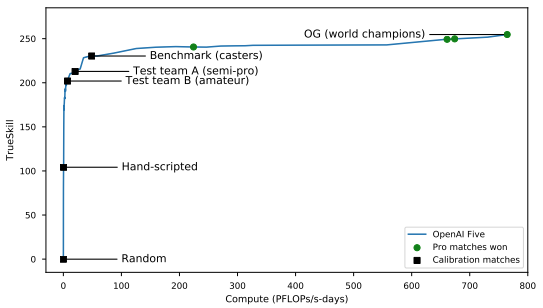
\includegraphics[scale=0.65]{images/trainingsverlauf_openai.png}
\caption{Trainingsverlauf OpenAI Five \cite{openai_five_paper}}
\label{fig:trainingsverlauf_openai}
\end{figure}

Bei dem auf der y-Achse verzeichneten \Fachbegriff{TrueSkill}-Wert handelt es sich um eine im Jahr 2007 vorgestellte Metrik für die Einschätzung des Skill-Levels in kompetitiven Spielen \cite{NIPS2006_3079}. Die Grafik zeigt einen zunächst drastischen Anstieg aufgrund der exponentiellen Natur des Problems, sodass bereits nach sehr kurzer Zeit semiprofessionelle Teams geschlagen werden konnten. Das ist bereits eine sehr aussagekräftige Metrik, da auch semiprofessionelle menschliche Spieler jahrelanges intensives Training absolvieren müssen, um dieses Level zu erreichen. Der anschließende Verlauf ist nur sehr leicht steigend. Verbesserungen zum Ende des Verlaufs wurden mit der Einführung weiterer Fähigkeiten, die der KI zuvor nicht verwenden konnte, begründet, sodass schließlich auch das aktuell beste menschliche Team geschlagen werden konnte.

Es zeigt sich, dass selbst überaus komplexe Spiele und damit schwierige Probleme mit \ac{reinforcement_learning} gemeistert werden können. Sie beweisen zum Einen die Skalierbarkeit klassischer Machine Learning-Methoden und zum Anderen die Möglichkeit, Agenten in Verbindung mit einer großen Menge von Rechenleistung übermenschliche Fähigkeiten zu verleihen. Dabei dienen Videospiele als eine Art \sogenannt{Spielplatz} für das Experimentieren und Forschen mit Machine Learning-Verfahren, da diese eine optimale Umgebung dafür bieten.


%- openAI hide and seek --> sehr interessante, unerwartet verhaltensmuster

% Hide and seek
    % https://www.quantamagazine.org/artificial-intelligence-discovers-tool-use-in-hide-and-seek-games-20191118/


% neuer ansatz: statt experience learning multi agent ansatz:
% http://proceedings.mlr.press/v48/mniha16.pdf

% https://hciweb.iwr.uni-heidelberg.de/system/files/private/downloads/541645681/dammann_reinfocement-learning-report.pdf


%- veränderung in den letzten jahren?
%- altbewährte systeme wie decision trees immernoch nützlich?


\section{Potential}
Die oben genannten Beispiele zeigen, dass es eine Vielzahl von Anwendungsfällen für Machine Learning in Videospielen gibt. Neben der Verbesserung intelligenter Agenten sind auch andere Bereiche relevant, die zur Erschaffung von Welten mit einer erhöhten Glaubwürdigkeit und Authentizität beitragen können. Die genannten Spiele zeigen, wie kreativ lernende Agenten in sehr unterschiedlichen Bereichen eingesetzt werden können und welche interessante Szenarien damit vorstellbar sind. Die Nutzung in Strategiespielen beweist darüber hinaus die Skalierbarkeit der Verfahren. Sie ermöglichen eine Interaktion mit dem Spieler, die mit klassischen Verfahren nicht realisierbar ist und erzeugen so authentische Spielerlebnisse.

Der Entwickler von \Fachbegriff{Supreme Commander 2} und \Fachbegriff{Planetary Annihilation}, nennt eine Menge von Vorteilen, die sich direkt aus der Nutzung eines neuronalen Netzes ergeben:

\begin{itemize}
    \item \texttt{Gewichtung der Inputs}: Eine Gewichtung der Inputs fällt weg.
    \item \texttt{Wichtigkeit der Inputs irrelevant}: Wenn irrelevante Inputs vorhanden sind, sollte das System davon nicht beeinflusst werden.
    \item \texttt{Vergleichbarkeit der Zustandsvariablen}: Es ist nicht nötig, die einzelnen Werte miteinander zu vergleichen. Wäre dies nicht der Fall, so müsste ein Weg gefunden werden, um beispielsweise Inputvariablen wie \textit{Geschwindigkeit} und \textit{Schaden} vergleichen zu können.
    \item \texttt{Kein Algorithmus nötig}: Es muss kein Algorithmus entwickelt werden, der das genaue Verhalten der Einheiten beschreibt.
\end{itemize}

Laut Robbins bestehe ein großer Vorteil also darin, dass fast beliebige Werte als Inputvariablen für das neuronale Netz verwendet werden können. Das neuronale Netz kümmere sich dann anstelle des Entwicklers von selbst um die Normalisierung und den Vergleich der Variabeln. Weiterhin sei es nicht nötig das Verhalten der Agenten direkt zu beschreiben, sodass insgesamt viel Arbeitszeit gespart wird.

Im Allgemeinen können außerdem Kosten gespart werden, indem Inhalte generiert werden, anstatt dafür einen hohen Arbeitsaufwand aufzubringen. Besonders bei der Nutzung intelligenter Agenten besteht das Potential, den massiven Zeitaufwand des Scriptings zu reduzieren, indem beispielsweise Reinforcement Learning genutzt wird. Das Verhalten der Agenten muss dann nicht explizit definiert werden, weil es \Fachbegriff{erlernt} wird.
Die Menge der Inhalte, die für ein erfolgreiches Spiel nötig sind, sollten dabei nicht unterschätzt werden. Im 2018 erschienenen Spiel \Fachbegriff{Red Dead Redemption 2} \cite{rdr2} wurden allein etwa 300.000 Charakter- und Tieranimationen angefertigt bzw. aufgenommen \cite{rdr2_script_pages}. Dadurch kann ein guter Eindruck darüber gewonnen werden, wie viel Zeit und Geld durch eine prozedurale Generierung von Animationen gespart werden könnte.
Aktuelle Entwicklungen beweisen ein vielversprechendes Potential, da selbst in komplexen Szenarien menschenähnliches oder sogar übermenschliches Verhalten erlernt werden kann. Reinforcement Learning zeigt, dass auch mit altbewährten Algorithmen erstaunliche Ergebnisse erreicht werden können, die in hohem Maße und durch den erhöhten Einsatz von leistungsfähiger Hardware skalierbar sind. Das lässt für die Entwicklung von NPCs vermuten, dass ebenfalls menschenähnliches Verhalten nachgeahmt werden kann, um die Immersion virtueller Welten zu erhöhen.
 \chapter{ML-Agents Toolkit}\label{ml_unity}

% allgemeiner kram:
% https://github.com/Unity-Technologies/ml-agents/blob/master/docs/ML-Agents-Overview.md
% https://unity3d.com/de/how-to/unity-machine-learning-agents

In diesem Kapitel wird das Unity-Framework \Fachbegriff{ML-Agents} für die Entwicklung intelligenter Agenten auf der Grundlage von Reinforcement Learning vorgestellt. Der erste Abschnitt befasst sich mit einer Einleitung in die Unity-Engine. Anschließend werden der Aufbau und die Funktionsweise von ML-Agents skizziert und anhand einer Beispielimplementierung verdeutlicht. 

\section{Unity}
\Fachbegriff{Unity} ist eine State-of-the-Art Echtzeit-Entwicklungsplattform der Firma \Fachbegriff{Unity Technologies} für 3D-Simulationen und wird neben Teilbereichen wie Architektur und Industrie hauptsächlich für den Games-Bereich verwendet \cite{unity}. Zahlreiche Zielplattformen wie \Fachbegriff{Microsoft Windows} und diverse Spielekonsolen werden unterstützt. Unity liefert Features wie eine weit entwickelte Grafik- und Physik-Engine sowie einen modifizierbaren Editor für die Realisierung komplexer Projekte. Mit dem Editor können sämtliche gängigen Prozesse aus der Spieleentwicklung genutzt werden, beispielsweise aus den Bereichen \aufzaehlung{Networking} oder \aufzaehlung{Asset-Management}. Unity's eingebaute Mechanismen werden dabei durch Scripte ergänzt, um die Logik von Spielen zu implementieren. Abbildung \ref{fig:unity_heretic_demo} zeigt eine Momentaufnahme aus einer in Echtzeit berechneten Unity-Techdemo, um die Möglichkeiten der Engine zu verdeutlichen.

\begin{figure}[H]
\centering
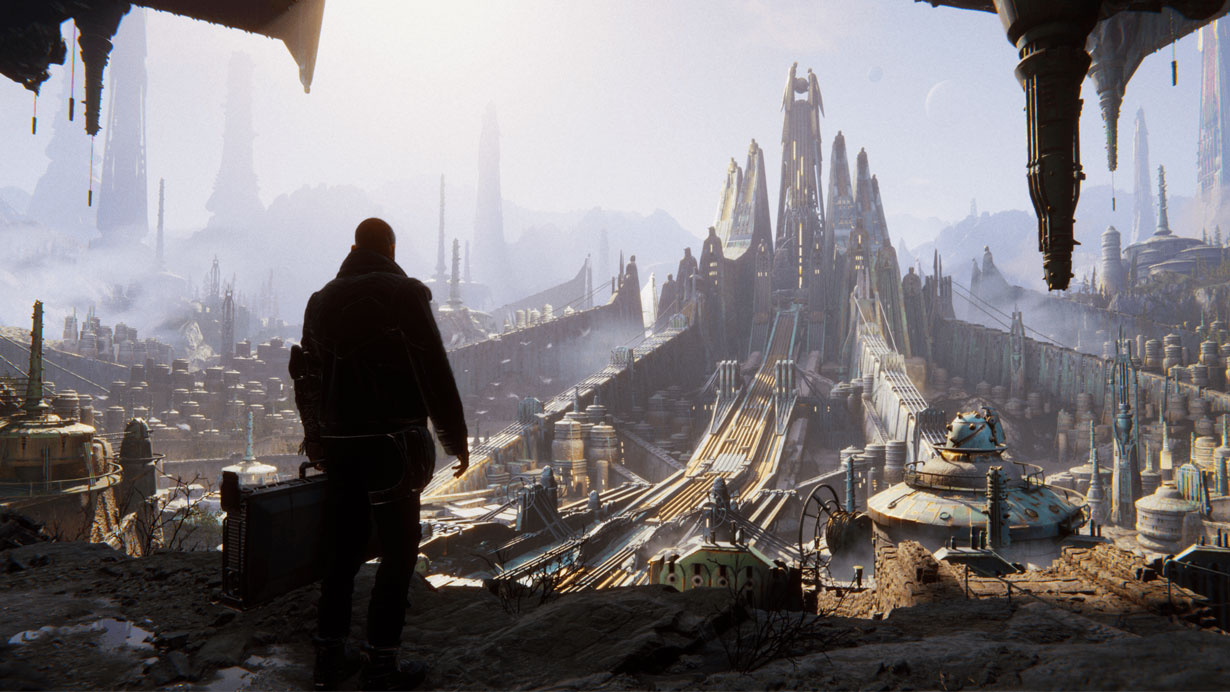
\includegraphics[scale=0.3]{images/ml-agents/unity_heretic_demo.jpg}
\caption{Unity-Echtzeitgrafik in \Fachbegriff{The Heretic} \cite{unity_heretic}}
\label{fig:unity_heretic_demo}
\end{figure}

Unity wendet sich sowohl an semiprofessionelle als auch hauptberufliche Spieleentwickler und große Entwicklerstudios. Mit einem Marktanteil von etwa 48\% im Vergleich zu den lediglich 13\% der \Fachbegriff{Unreal Engine} stellt sie die mit Abstand verbreiteteste Game Engine dar \cite{unity_marktanteil}.

\paragraph{Grundlagen}\label{scripting_unity_basics}
Unity verwendet die Programmiersprache C\# und erweitert diese um zusätzliche Konzepte, die speziell für die Entwicklung von Spielen vorgesehen sind. Alle in der Spielszene verwendeten Entitäten - unabhängig davon, ob sie über eine visuelle Repräsentation verfügen - basieren auf sogenannten \Fachbegriff{GameObjects}. Sie dienen als fundamentale Container, denen beliebig viele Komponenten hinzugefügt werden können. Scripts, die direkt an ein GameObject gebunden werden, heißen \Fachbegriff{MonoBehavior} und unterstützen eingebaute Funktionen der Engine wie beispielsweise die Funktion \inlinecode{Update}, die mit jedem neuen Frame aufgerufen wird. Komplexe hierarchische Konstrukte von \Fachbegriff{GameObjects} können anhand von sogenannten \Fachbegriff{Prefabs} zu Vorlagen transformiert werden, die auf der Festplatte gespeichert werden. Prefabs erlauben die Änderung von allen Objekten eines Typs durch die simple Anpassung des Basisobjekts. Weiterhin können große Mengen von Objekten desselben Typs leicht instantiiert werden.
Ein weiteres wichtiges Konzept sind \Fachbegriff{Coroutines}, welche in der Lage sind, die Ausführung einer Methode anzuhalten, um auf ein Ergebnis zu warten \cite{unity_coroutines}. Das geschieht mit dem Stichwort \Fachbegriff{yield}. Weiterhin können Coroutinen eigene Threads zugewiesen werden, indem \Fachbegriff{AsyncCoroutines} verwendet werden. Coroutines geben ein Ergebnis vom Typen \Fachbegriff{IEnumerator} zurück. Dieser Typ ist nicht Unity-basiert, sondern stammt aus dem \Fachbegriff{Microsoft .NET}-Framework. Coroutinen können nur von Monobehaviors durch die Funktion \Fachbegriff{StartCoroutine} und \Fachbegriff{StartCoroutineAsync} gestartet werden.


\paragraph{Unity Editor}
Unity liefert einen umfangreichen Editor für die Entwicklung von Spielen und Simulationen. Bis auf die Anfertigung von Assets und der Entwicklung von Programmcode finden alle Vorgänge zur Entwicklung eines Spiels in Unity selbst statt. Scripts werden in einer externen C\#-fähigen IDE entwickelt, wie zum Beispiel Visual Studio oder vergleichbaren Anwendungen. Ebenso werden Modelle und Grafiken in externen Anwendungen angefertigt.
Der Editor arbeitet szenenbasiert, wobei jede Szene ein eigenständiges Level darstellt. Im Verlauf dieser Arbeit wurde lediglich eine Szene für die Simulation des Dorfes entwickelt. Mit der Anwendung werden die folgenden Aufgaben bearbeitet:

\begin{itemize}
    \item Verwaltung eines komponentenbasierten Systems, Erzeugung und Manipulation von GameObjects 
    \item Bereitstellung einer Engine für physikalische Vorgänge wie Bewegungen, Kollisionen, etc.
    \item Rendering der Szene, Möglichkeit der Nutzung von Render-Pipelines
    \item Gestaltung des Levels mit visuellen Komponenten wie Mesh, Shadern, Texturen, Beleuchtung, Partikel, etc.
    \item Grundlegende Erzeugung und Manipulation weiterer Assets wie Sounds und Animationen (häufig in externen Programmen gelöst)
    \item Nutzung von Programmcode durch Scripts
    \item Verwaltung von Assets wie Sounds, Grafiken und 3D-Modellen
    \item Bereitstellung von speziellen Features wie Pathfinding und Leistungsoptimierungen wie \Fachbegriff{Occlusion Culling} \cite{unity_occlusion_culling}
    \item Bereitstellung diverser Plugins zur Erweiterung des Editors in beliebigen Bereichen
    \item Profiling und Debugging der Anwendung
    \item Ausspielen der Anwendung auf verschiedene Plattformen
\end{itemize}


Die Oberfläche des Editors wird in der Abbildung \ref{fig:unity_editor_overview} gezeigt. Das Bild zeigt die fundamentalen Komponenten des Editors.

\begin{figure}[H]
\centering
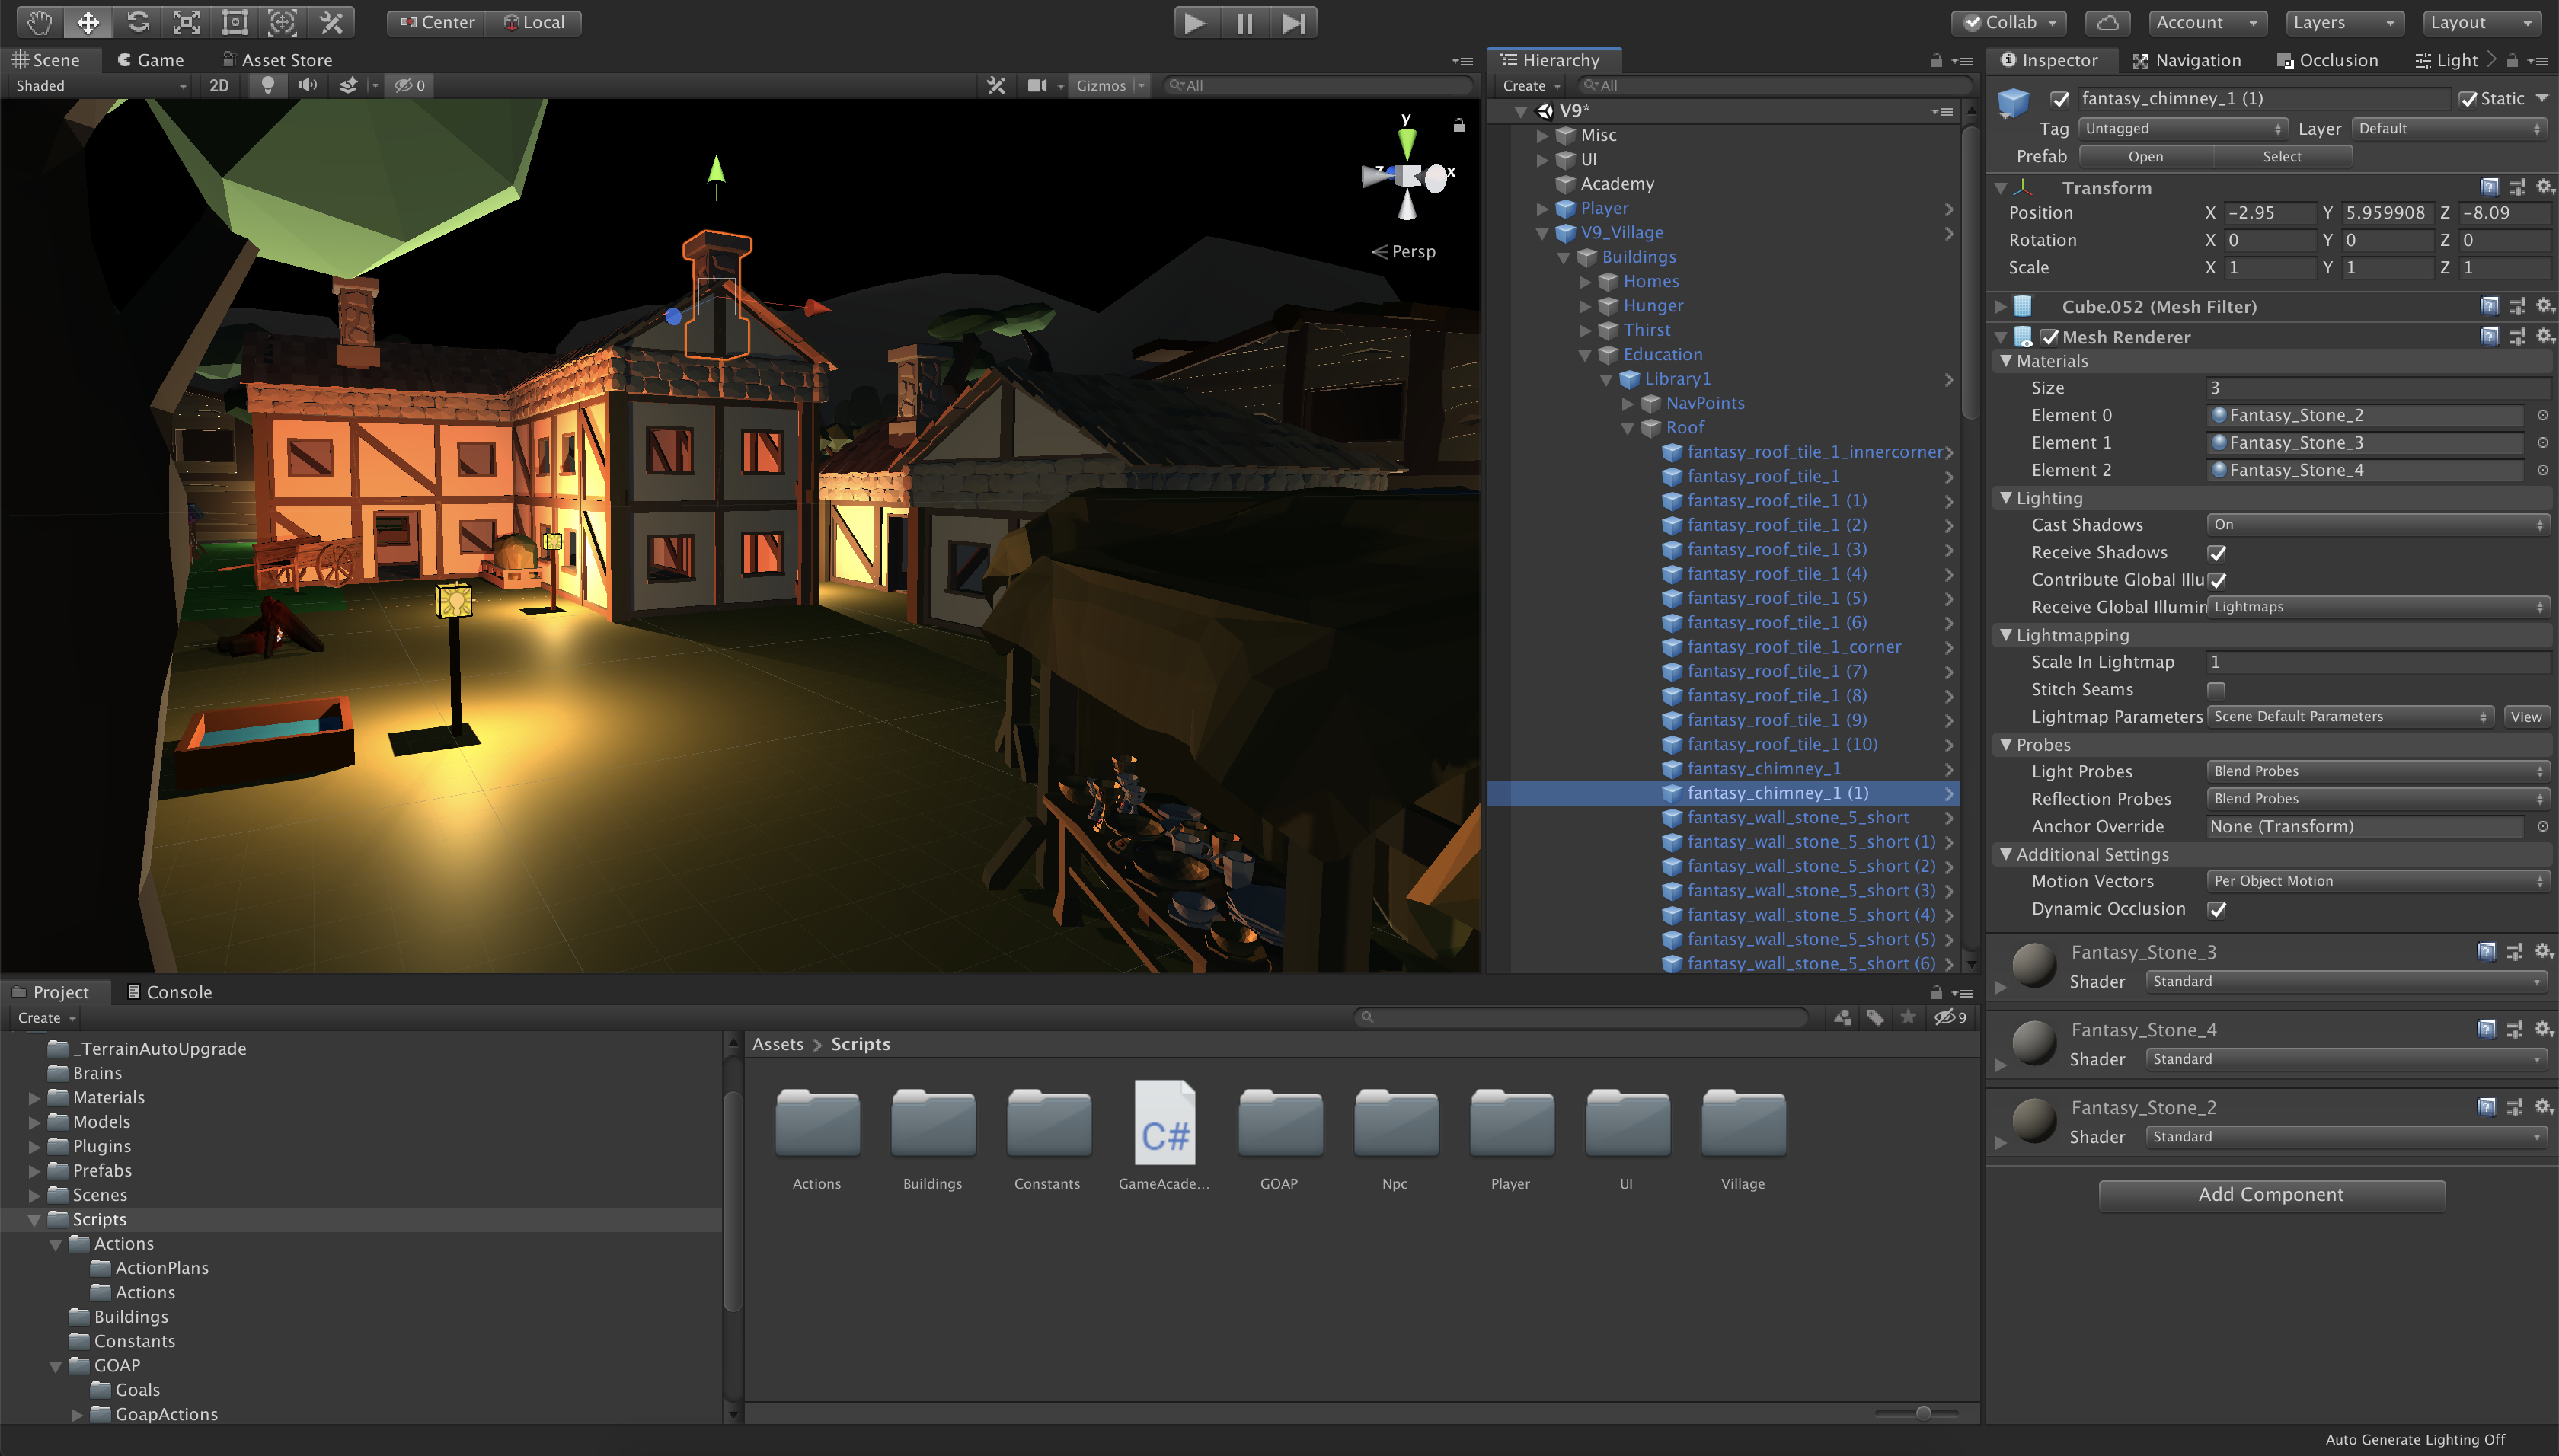
\includegraphics[scale=0.277]{images/ml-agents/unity_editor_overview.png}
\caption{Oberfläche des Unity Editors}
\label{fig:unity_editor_overview}
\end{figure}

Auf der rechten Seite ist der \Fachbegriff{Inspector} zu erkennen, der die Inspektion sowie das Hinzufügen und die Manipulation von Komponenten eines GameObjects erlaubt. Der Inspector zeigt die Komponenten des in der Szene ausgewählten GameObjects, die auf der linken Seite zu sehen ist und in der navigiert werden kann. In der Mitte der Abbildung ist die Szenenhierarchie zu erkennen, die den Aufbau der Szene beschreibt und Abhängkeiten von GameObjects definiert. Der untere Bereich zeigt die Ordnerstruktur des Projekts mit Assets, Scripts, Bibliotheken etc.
Ein großer Vorteil von Unity ist weiterhin die Möglichkeit, entwickelte Spiele direkt im Editor auszuführen, ohne dass Build-Vorgänge für spezifische Zielplattformen notwendig sind. Änderungen in der Szene oder im Programmcode können daher schnell getestet werden.



\subsection{Machine Learning in Unity}
Vor der Einführung von ML-Agents musste für die Nutzung von Machine Learning in Unity ein deutlich höherer Aufwand betrieben werden, da ausschließlich Community-Plugins verfügbar waren. Diese wurden sowohl genutzt, um eine Verbindung zu externen Schnittstellen wie Tensorflow aufzubauen, oder aber, um selbst neuronale Netzwerke zu implementieren. Da diese jedoch lediglich von Nutzern aus der Unity-Gemeinschaft entwickelt wurden, bestand aufgrund offensichtlicher Nachteile kein großes Interesse an der Verwendung von Machine Learning in Unity. Mit der Entwicklung des \Fachbegriff{ML-Agents Toolkit} wird der Einstieg in die Nutzung von Machine Learning in Unity extrem vereinfacht. Das Framework wird im folgenden Abschnitt näher skizziert.


\section{ML-Agents-Architektur}
\Fachbegriff{ML-Agents} ist ein von Unity Technologies entwickeltes Open-Source Framework, das Spielen und Simulationen erlaubt, als Entwicklungs- und Testumgebung für lernende Agenten zu fungieren \cite{ml-agents_paper} \cite{ml-agents_documentation} \cite{ml-agents_github}. Es befindet sich aktuell in der Beta-Phase, verfügt aber bereits über alle grundlegenden Features und ist öffentlich nutzbar. Mit ML-Agents wurde eine Plattform geschaffen, die die Entwicklung von lernenden Agenten einer größeren Menge von Entwicklern zugänglich machen, da sie vorhandene Hürden abbaut und den nötigen Aufwand reduziert.

In der Regel wird ML-Agents in der Kombination mit Imitation Learning oder Reinforcement Learning verwendet (siehe Abschnitte \ref{imitation_learning} und \ref{reinforcement_learning_intro}). Andere Verfahren wie genetische Algorithmen (z.B. \Fachbegriff{NeuroEvolution}), können ebenfalls verwendet werden, sind aber weniger gut dokumentiert und weniger üblich. Für den Trainingsvorgang stellt das Framework eine Verbindung zu einer Python-API her. Verschiedene State-Of-The-Art-Algorithmen wie \ac{ppo} und \ac{sac} werden dem Nutzer zur Verfügung gestellt. Das genaue Anwendungsszenario des Frameworks bleibt dabei dem Entwickler überlassen; es kann sowohl für die Verhaltenssimulation von NPCs als auch für automatisierte Tests oder der Evaluation des Game Designs verwendet werden \cite{ml-agents_github}. Ml-Agents bietet eine intuitive Architektur sowie eine große Menge von veränderbaren Parametern, um eine flexible Entwicklung von Agenten zu gewährleisten. Im Folgenden wird das Framework ausschließlich in der Kombination mit Reinforcement Learning verwendet.




\subsection{Grundlegende Funktionsweise}
Zur Installation wird ein \inlinecode{git clone} des ML-Agent GitHub-Archivs \cite{ml-agents_github} in ein leeres Unity-Projekt durchgeführt. Zusätzlich wird das \inlinecode{mlagents} Python Package benötigt. Diverse Beispiele sind bereits im Projekt enthalten und können zum Verständnis verwendet werden. Alternativ wird die Verwendung eines Docker-Image angeboten.

\begin{figure}[H]
\centering
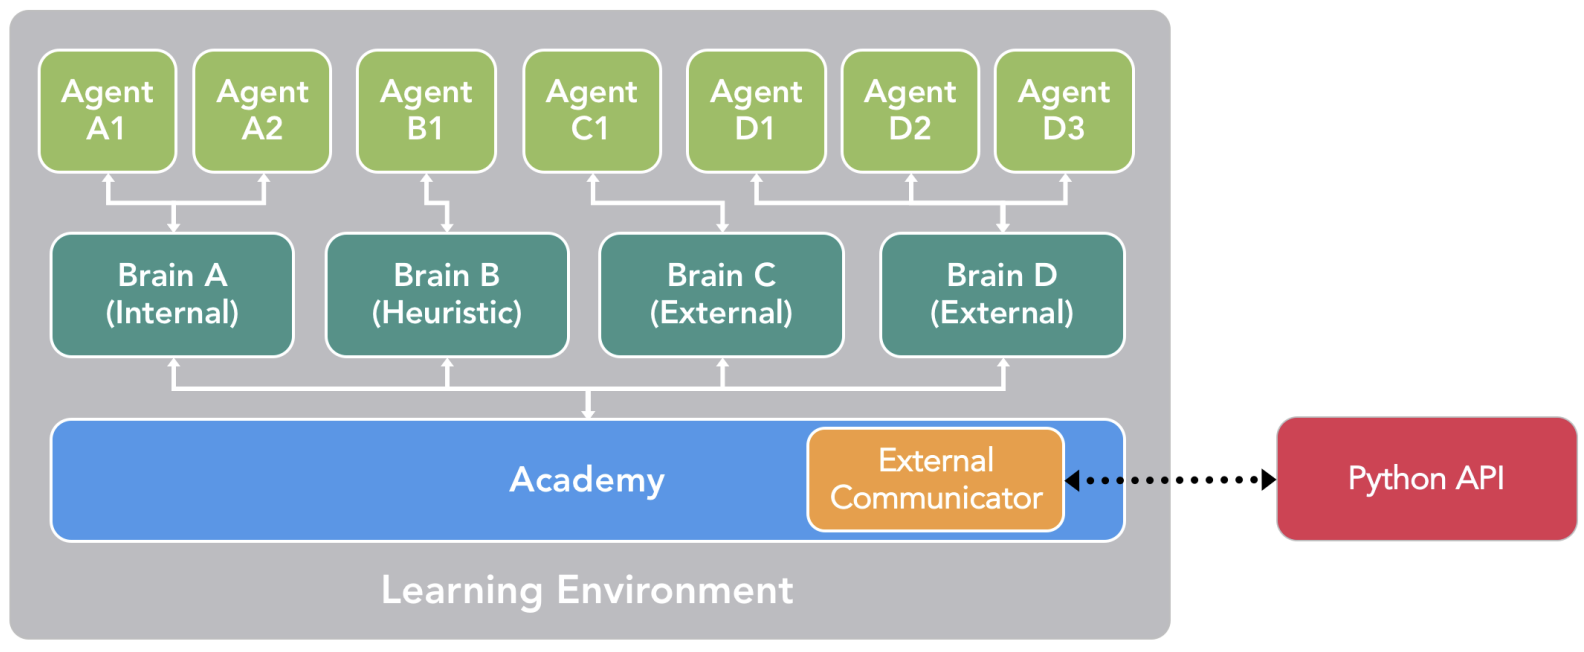
\includegraphics[scale=0.575]{images/ml-agents/architecture.png}
\caption{ML-Agents Architektur \cite{ml-agents_documentation}}
\label{fig:ml-agents_architecture}
\end{figure}

Vier grundlegende Klassen müssen in einem ML-Agents-Projekt verwendet werden, um einen lernenden intelligenten Agenten zu entwickeln. Im Einzelnen handelt es sich dabei um die folgenden zu implementierenden Konzepte, zu denen eine kurze Übersicht geliefert wird.

\newpage
\begin{itemize}
    \item \texttt{Agent}: Sammelt Observations und führt Aktionen aus.
    \item \texttt{Brain}: Das Gehirn der AI, trifft Entscheidungen.
    \item \texttt{Academy}: Zentrale Verwaltung aller Brains, externe Verbindung zu Python.
    \item \texttt{Model}: Resultat des Lernvorgangs, enthält Policy für ein Brain.
\end{itemize}

Die Abbildung \ref{fig:ml-agents_architecture} zeigt die zugrunde liegende Architektur, die die erwähnten Komponenten beinhaltet. Im Folgenden wird die Funktionsweise der einzelnen Konzepte beschrieben. Weiterhin wird näher darauf eingegangen, was bei einer Implementierung zu beachten ist.




\subsection{Academy}
Die Academy ist für die globale Koordinierung der Simulation zuständig. Sie dient als eine zentrale Verwaltungseinheit für alle Agenten und Brains. Durch die Herstellung der Verbindung zu einer externen Schnittstelle in Form eines Tensorflow-Backends stellt sie zusätzlich die Trainingsumgebung dar. Jegliche Machine Learning-Vorgänge sind vom eigentlichen Unity-Projekt völlständig entkoppelt, da der Entscheidungsprozess in Python abläuft.

Um Entscheidungen für Agenten zu treffen, findet eine kontinuierliche Kommunikation zwischen der Academy und der Python-API über den \Fachbegriff{External Communicator} statt (siehe Abbildung \ref{fig:ml-agents_architecture}), indem die Observations der Agenten an Tensorflow weitergeleitet werden. Tensorflow verfügt dabei über alle für das Training verwendeten Machine Learning-Algorithmen. Ein neuronales Netz innerhalb des Backends erzeugt einen Output, der die Entscheidung des Agenten in Abhängigkeit von den zuvor gesammelten Observations darstellt. Dieser Vorgang gilt sowohl für den Trainings- als auch für den Inference-Vorgang.

Zum Beginnn der Ausführung ruft die Academy die Funktion \inlinecode{AgentReset} für alle Agenten auf. Anschließend werden alternierend die Funktionen \inlinecode{CollectObservations} und \inlinecode{AgentAction} aufgerufen. Jeder Vorgang beinhaltet die Erzeugung einer Entscheidung durch das neuronale Netz und die Ausführung der entsprechenden Aktion durch den Agenten. Dies wird solange wiederholt, bis der Agent eine Episode abgeschlossen hat oder die maximale Schrittweite erreicht wurde. Anschließend wird der Prozess mit dem Aufruf von \inlinecode{AgentReset} erneut gestartet.

\subsection{Agent}
% https://github.com/Unity-Technologies/ml-agents/blob/master/docs/Learning-Environment-Design-Agents.md
Um einen neuen Agenten zu erzeugen, muss eine neue Klasse angelegt werden, die von der Oberklasse \Fachbegriff{Agent} erbt. Diese beschreibt die grundsätzlichen Aufgaben und nötigen Vorgänge eines lernenden Agenten. \Fachbegriff{Agent} erbt von der Unity-Basisklasse Monobehavior und verfügt daher über automatisch verwaltete Funktionen wie \Fachbegriff{Update} (siehe Abschnitt \ref{scripting_unity_basics}). Jeder Agent wird daher an ein GameObject angehängt. Folgende Funktionen müssen implementiert werden:

\newpage
\begin{itemize}
    \item \inlinecode{InitializeAgent}: Beinhaltet die einmalige Initialisierung des Agenten.
    \item \inlinecode{CollectObservations}: Vor jeder Aktion müssen Observations aus der Umgebung des Agenten gesammelt werden. Das können beispielsweise die Position des Agenten und eines Ziels oder dessen Lebenspunkte sein. Beobachtungen werden gesammelt, indem \inlinecode{AddVectorObs} aufgerufen wird. Diese Funktion unterstützt Zahlenwerte, Vektoren, Strings und Boolsche Werte. Weiterhin besteht die Möglichkeit, visuelle Beobachtungen zu verwenden. In dieser Arbeit wird diese Option nicht weiter behandelt.
    \item \inlinecode{AgentAction}: Die Parameter der Funktion beschreiben den Output des neuronalen Netzes. Der Agent muss entsprechend darauf reagieren und die jeweiligen Aktionen ausführen.
    \item \inlinecode{AgentReset}: Damit wird der Agent inklusive etwaiger Abhängigkeiten zurückgesetzt. Soll der Agent beispielsweise lernen, auf einer Plattform zu balancieren, so würde er beim Fallen von der Plattform wieder auf dieser platziert werden. Zusätzlich könnte die Plattform wieder horizontal ausgerichtet werden. \inlinecode{AgentReset} wird automatisch aufgerufen, wenn eine Episode endet, indem \inlinecode{Done} aufgerufen wird.
\end{itemize}

Essentiell sind die Funktionen \texttt{CollectObservations} für das Sammeln von Beobachtungen und \texttt{AgentAction}, um zu bestimmen, welche Aktion gewählt werden soll. Bei der Entscheidung der Aktionen kann zwischen zwei Szenarien gewählt werden. 

Bei den \Fachbegriff{diskreten} Entscheidungen wird anfangs eine Menge von möglichen Entscheidungen festgelegt, denen ein Index zugewiesen wird. In den Parametern von \inlinecode{AgentAction} wird dann ein einzelner Wert übermittelt, der eine ausgewählte spezifische Aktion referenziert, die ausgeführt werden soll. Der Output des neuronalen Netz bestimmt also die Ausführung einer bestimmten Aktion, indem ein ausgewählter Index für eine Aktion übermittelt wird. Diese Indizes werden durch Integer dargestellt, die bei $0$ aufsteigend beginnen.
Bei den \Fachbegriff{kontinuierlichen} Entscheidungen hingegen wird in jedem Fall für alle festgelegten Aktionen je ein Wert geliefert. Dabei werden keine Indizes, sondern skalare Werte anhand von Floats übermittelt, die die Amplitude für die jeweiligen Aktionen bestimmen. Diese haben einen Zahlenbereich von $-1$ bis $+1$. Ein mögliches Anwendungsszenario ist die Bewegung eines virtuellen Charakters. Es werden drei Aktionen festgelegt, um den Agenten erstens vor- und rückwärts und zweitens seitwärts zu bewegen. Die dritte Aktion bestimmt die Rotation des Agenten. Die Amplitude bestimmt nun, wie stark der Agent in eine Richtung bewegt oder gedreht werden soll, bzw. in welche Richtung er dabei vorgehen soll. Anstatt sich für eine Aktion zu entscheiden wird jeder möglichen Aktion also ein skalarer Wert zugewiesen, die den kontinuierlichen Ausschlag für die damit assoziierte Aktion bestimmt.


Eine essentielle Aufgabe des Agenten ist darüber hinaus die Erzeugung von Belohnungen. Die Funktion \inlinecode{AddReward} nimmt einen positiven oder negativen Float-Wert, der eine Belohnung oder eine Bestrafung darstellt. Es handelt sich also um einen skalaren Wert der beschreibt, wie gut der Agent agiert (siehe Kapitel \ref{reinforcement_learning}). Das mehrfache Aufrufen von \inlinecode{AddReward} führt zu einer Akkumulierung der Belohnungen. Außerdem besteht die Möglichkeit, den Reward direkt über \inlinecode{SetReward} festzulegen, wodurch bisherige Belohnungen für die ausgeführte Aktion ignoriert werden. Beim Training werden diese Belohnungen genutzt, um Beziehungen zwischen dem Spielzustand und den möglichen Aktionen herzustellen.

Zu Testzwecken können Entscheidungen vom Spieler selbst bestimmt werden. Dafür muss die Funktion \inlinecode{Heuristic} in der Agentenklasse überschrieben werden. Die Aktionen des Agenten werden dann nicht durch das Brain, sondern vom Spieler selbst bestimmt, indem den Aktionen Tastaturbefehle zugewiesen werden. Vor dem Training können so leicht Fehler entdeckt und die Funktionsweise eines Agenten getestet werden.

\subsection{Brain}
Zwischen der Academy und den Agenten existiert eine weitere zwischengeschaltete Entität namens \Fachbegriff{Brain}. Ein Brain kann beliebig viele Agenten verwalten (sieht Abbildung \ref{fig:ml-agents_architecture}). Jeder dieser Agenten verfügt über eine Referenz auf das Brain. Die Aufgabe des Brains ist die Bereitstellung einer Policy oder \Fachbegriff{Model} für alle mit ihm assoziierten Agenten und die Weiterleitung von Observations und Entscheidungen zwischen den Agenten und der Academy. Für jedes Brain wird im Tensorflow-Backend ein eigenes neuronales Netz angelegt.
Im Trainingsmodus werden für jedes Brain seperate Hyperparameter anhand einer Konfigurationsdatei zur Verfügung gestellt, die die Beschaffenheit des zugrunde liegenden neuronalen Netzes bestimmen. Jedes Brain wird außerdem über Parameter konfiguriert, die beispielsweise die Anzahl der Beobachtungen oder die Anzahl der möglichen Aktionen festlegen. Auch der Ablauf des Entscheidungsprozesses kann durch Parameter verändert werden: Standardmäßig wird nach einer festlegbaren Anzahl von Zeitschritten automatisch eine neue Entscheidung angefragt. Alternativ können sogenannte \Fachbegriff{On Demand Decisions} verwendet werden. Der Agent beantragt dann selbst eine neue Entscheidung, wenn seine vorherige Entscheidung abgeschlossen ist. Dies ist zum Beispiel nützlich, wenn die Dauer der Aktionen nicht absehbar ist.

\subsection{Model}
Beim \Fachbegriff{Model} handelt es sich um eine Policy bzw. ein Modell, das aus dem Trainingsvorgang eines Agenten hervorgegangen ist. Eine Policy ist nichts weiteres, als die Beschreibung der Parameter $\theta$ eines neuronalen Netzes, also der Gewichtungen der Neuronen. Für den Inference-Modus muss jedes verwendete Brain über ein \Fachbegriff{Model} verfügen. Ein Agent führt dann Aktionen aus, die das fertige Model aufgrund der Beobachtungen bereitstellt, ohne dass ein Trainings- oder Lernvorgang stattfindet.

Da die Parameter des Brains wie beispielsweise die Anzahl der Beobachtungen und möglichen Aktionen die Struktur des zugrunde liegenden neuronalen Netzes beeinflusst, ist das Model von ihnen abhängig. Sobald Parameter eines Brains verändert werden, kann ein trainiertes Model nicht mehr verwendet werden. In diesem Fall muss ein neuer Trainingsvorgang erfolgen.



\subsection{Training}
Während des Vorgangs versenden die Brains Observations der mit ihnen verknüpften Agenten über den External Communicator an die Python API und erhalten Aktionen als Antwort zurück. Innerhalb von Tensorflow findet dann der Lernprozess statt, in welchem die beste Policy für das jeweilige Brain gefunden wird. Nach dem Training wird das gelernte Model anhand einer Tensorflow Model-Datei mit der Endung \textit{.nn} gespeichert. Das Training kann sowohl mit nur einem als auch mit mehreren Agenten und Brains ablaufen. Die Verwendung mehrere Agenten kann die Geschwindigkeit und Stabilität des Trainings erhöhen \cite{ml-agents_documentation}. Für das Training werden die Framerate des Spiels und die Qualität der visuellen Darstellungen reduziert. Weiterhin kann die sogenannte \Fachbegriff{Time Scale} verändert werden, um schnellere Aktionen von den Agenten zu provozieren. Die in Unity eingebaute Time Scale simuliert eine Beschleunigung der Zeit. Sämtliche physikalische Aktionen laufen dann schneller ab. Update-Funktionen werden noch immer im selben Abstand aufgerufen, da sie entweder von der Framerate oder einem festen Intervall abhängen. Die scheinbar vergangene Zeit, die in Unity mithilfe von \inlinecode{Time.deltaTime} aufgerufen werden kann, erhöht sich dann proportional zum Time Scale-Faktor. 

Um einen Trainingsvorgang zu starten, können Befehle des \Fachbegriff{mlagents} Python Package verwendet werden. Diese sind unter \filepath{ml-agents/mlagents/trainers/learn.py} zu finden. Wichtig ist außerdem, dass in der Academy die zu trainierenden Brains referenziert werden und jeweils die Flag \Fachbegriff{Control} gesetzt wird. Folgende Anweisung wird verwendet, um das Training zu starten:

\begin{center}
    \inlinecode{mlagents-learn <config-file> --env=<env\_name> --run-id=<some-id> --train}
\end{center}

Der Parameter \inlinecode{env\_name} bezieht sich auf den Pfad der kompilierten ausführbaren Unity-Simulation. Wenn der Parameter nicht gesetzt wird, erfolgt das Training im Unity Editor. Nach dem Training kann mit dem Befehl \inlinecode{tensorboard --logdir=summaries --port <port-id>} ein \Fachbegriff{Tensorboard} verwendet werden. Ein lokaler Webserver wird dann gestartet, über den man in Echtzeit eine Visualisierung des Trainingsverlaufs betrachten kann. Über das Tensorboard können außerdem bereits vorhandene Trainingsdurchläufe evaluiert werden. In Abbildung \ref{fig:ml-agents_tensorboard} ist ein Tensorboard-Beispiel zu sehen. Zahlreiche Informationen zum Ablauf der jeweiligen Vorgänge stehen zur Verfügung. Dabei können anhand von Diagrammen Metriken wie die Belohnung, die Anzahl der Aktionen pro Episode, die Entropie der Policy und Weitere eingesehen werden.

\begin{figure}[H]
\centering
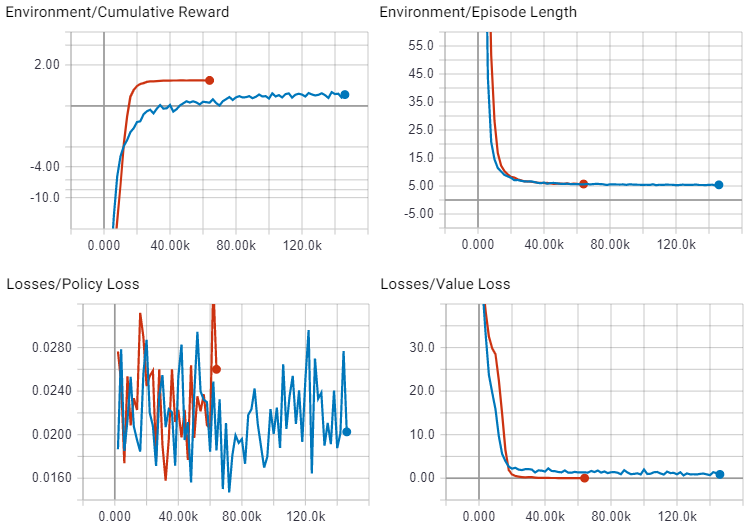
\includegraphics[scale=0.75]{images/ml-agents/tensorboard.png}
\caption{Tensorboard-Beispiel}
\label{fig:ml-agents_tensorboard}
\end{figure}

Weiterhin ist eine beispielhafte Konfigurationsdatei unter \filepath{config/trainer\_config.yaml} vorhanden. In dieser Konfiguration werden die Hyperparameter für das Training festgelegt. Dadurch kann unter anderem beschrieben werden, wie viele \Fachbegriff{Hidden Units}, also versteckte Neuronen, das neuronale Netz in wie vielen Schichten jeweils enthalten soll, oder auf welchen Wert die Lernrate festgelegt wird. Im Kapitel \ref{agenten_training} werden die einzelnen Hyperparameter näher beschrieben. Die Tabelle \ref{tab:ml-agents_training_hyperparameters} demonstriert eine Übersicht über die relevanten Parameter.
% advanced stuff???
    % curriculum: https://github.com/Unity-Technologies/ml-agents/blob/master/docs/Training-Curriculum-Learning.md
    % LSTM: https://github.com/Unity-Technologies/ml-agents/blob/master/docs/Feature-Memory.md
    % generalized agents for robust training: https://github.com/Unity-Technologies/ml-agents/blob/master/docs/Training-Generalized-Reinforcement-Learning-Agents.md




\section{ML-Agents-Beispiel}
Bei der Einarbeitung in das ML-Agents Toolkit wurde aus Gründen des Verständnisses und der Interesse ein Beispielprojekt angefertigt. Anhand dieses Beispiels soll ein erweitertes Verständnis über die Funktionsweise des Frameworks entstehen. Das Projekt wird im Folgenden vorgestellt. Der Quellcode für das Projekt kann im dazugehörigen GitHub-Repository betrachtet werden \cite{thesis_github_project}.


\subsection{Aufgabe}
Das Projekt beinhaltet einen einzelnen Agenten in Form eines Balls. Dieser soll lernen, sich zu einem Ziel (\Fachbegriff{Target}) zu bewegen. Sobald der Agent das Ziel erreicht, erhält der Agent eine Belohnung $r = 1$ und das Ziel wird zu einem anderen Ort bewegt. Sowohl Agent als auch Target befinden sich auf einer Plattform, von der der Agent herunterfallen kann. In diesem Fall bekommt der Agent eine hohe Bestrafung $r = -1$ und die Episode wird zurückgesetzt. Eine weitere Bestrafung $r = -0.1$ wird jedes Mal vergeben, wenn der Agent sich in die falsche Richtung bewegt. Die Abbildung \ref{fig:ml-agents_example_scene_single} zeigt den simplen Aufbau der Szene.

\begin{figure}[H]
\centering
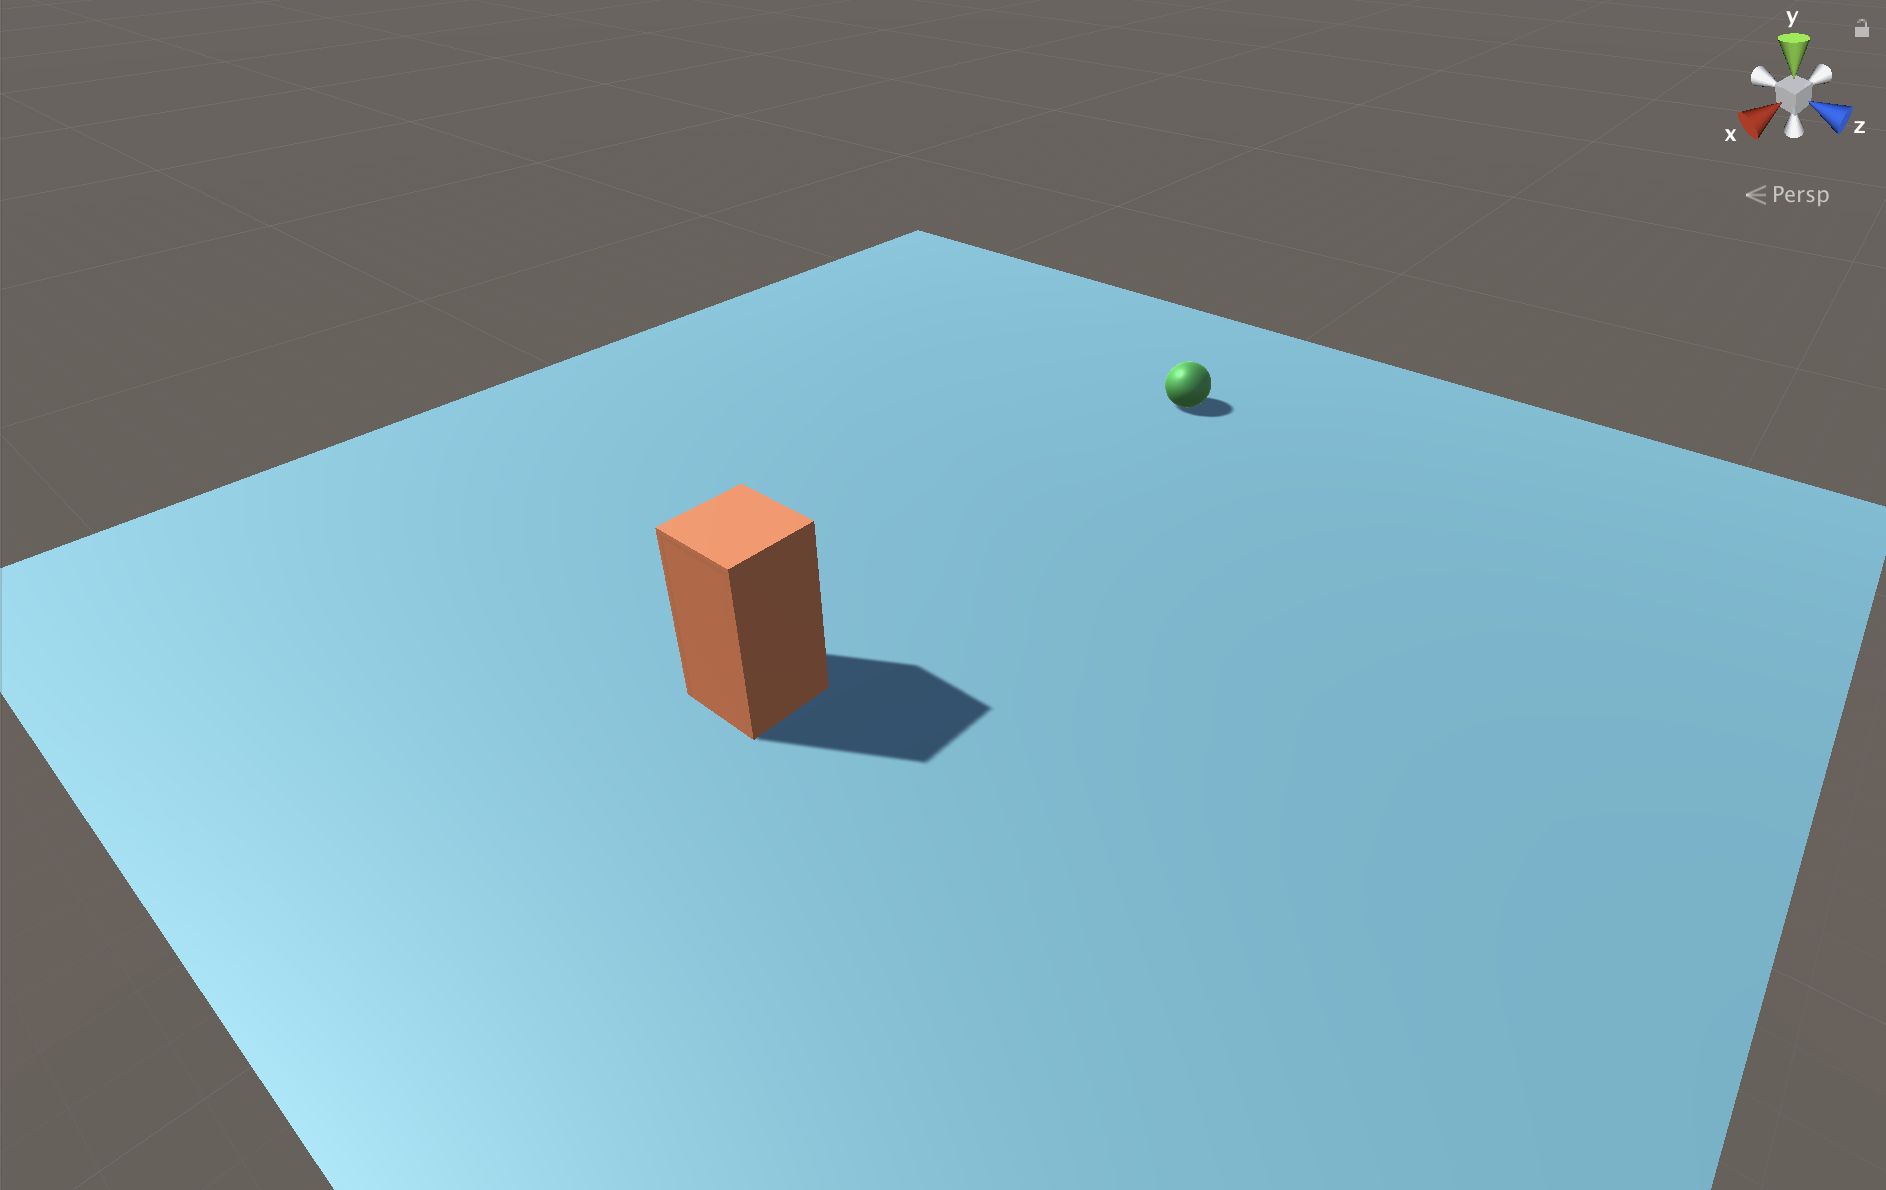
\includegraphics[scale=0.38]{images/ml-agents/example_scene_single.png}
\caption{ML-Agents-Beispiel, Aufbau der Szene}
\label{fig:ml-agents_example_scene_single}
\end{figure}


\subsection{Implementierung des Agenten}
Dieser Abschnitt zeigt, wie die einzelnen wichtigen Funktionen des Agenten implementiert wurden.

\paragraph{CollectObservations}
Das folgende Listing \ref{lst:ml-agents_example_observations} zeigt die Implementierung der Funktion \inlinecode{CollectObservations}. Die Wahl der Observations ist essentiell, damit sinnvolle Beziehungen zwischen Spielzustand und Belohnungswerten hergestellt werden können. Für die Lösung der Aufgabe sind vor allem die Position des Agenten und des Targets relevant, da der Agent sich darüber bewusst sein muss, in welche Richtung er sich bewegen muss (siehe Zeilen 3, 4, 8 und 9). Zusätzlich wird dafür die aktuelle Geschwindigkeit des Agenten verwendet. Diese wird von der \Fachbegriff{RigidBody}-Komponente bezogen, die GameObjects Interaktionen mit der Physik-Engine ermöglicht. Um Informationen darüber zu liefern, ob der Agent sich im Fallen befindet, wird weiterhin ein Boolscher Wert als Beobachtung hinzugenommen. Dadurch soll die Policy leichter eine Verbindung zu dem Grund der hohen erfahrenen Bestrafung erkennen können.

\begin{minipage}{\linewidth}
\begin{lstlisting}[linewidth=16.4cm, caption={ML-Agents-Beispiel, CollectObservations}, label=lst:ml-agents_example_observations, xleftmargin=1cm]
public override void CollectObservations() {
    AddVectorObs(this.transform.position.x);
    AddVectorObs(this.transform.position.z);
    AddVectorObs(_isAgentFalling());
    AddVectorObs(_agentRigidBody.velocity.x);
    AddVectorObs(_agentRigidBody.velocity.z);
    AddVectorObs(target.transform.x);
    AddVectorObs(target.transform.z);
}
\end{lstlisting}
\end{minipage}


\paragraph{AgentAction}
Zunächst wird ein Brain für den Agenten erstellt und konfiguriert, wie in Abbildung \ref{fig:ml-agents_example_brain_setup} erkennbar. Es soll ein kontinuierlicher Aktionsraum mit zwei Achsen verwendet werden, um den Agenten auf zwei Achsen zu bewegen. Für jede Aktion erhält der Agent dann zwei Werte, die seine Geschwindigkeit in X- und Z-Richtung beeinflussen. Weiterhin werden die in der Funktion \inlinecode{CollectObservation} getätigten Beobachtungen gezählt und eingetragen.

\begin{figure}[H]
\centering
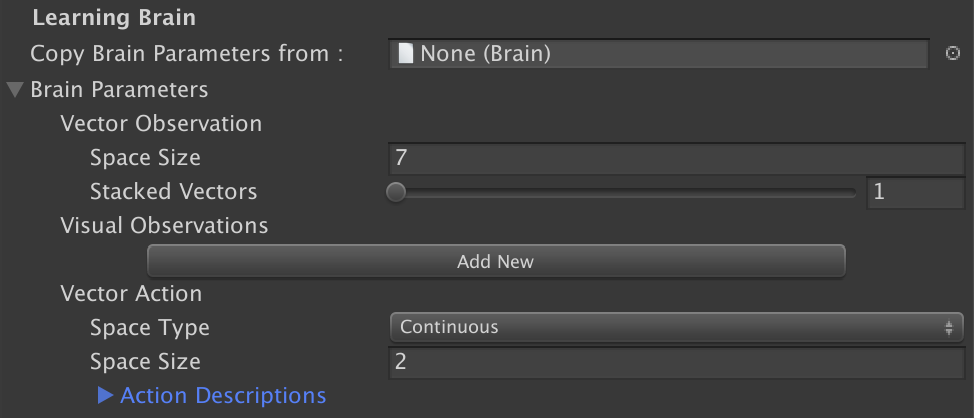
\includegraphics[scale=0.75]{images/ml-agents/example_brain_setup.png}
\caption{ML-Agents-Beispiel, Konfiguration des Brains}
\label{fig:ml-agents_example_brain_setup}
\end{figure}

Das folgende Listing \ref{lst:ml-agents_example_actions} zeigt die Aktionen, die der Agent ausführt, sowie die Verteilung der Belohnungen. Der Output des neuronalen Netzes wird in Form eines Float-Array zur Verfügung gestellt.

\begin{minipage}{\linewidth}
\begin{lstlisting}[linewidth=16.4cm, caption={ML-Agents-Beispiel, AgentAction}, label=lst:ml-agents_example_actions, xleftmargin=1cm]
public override void AgentAction(float[] vectorAction, string textAction) {
    // The agent fell off the edge. Finish episode with a punishment.
    if (_isAgentFalling()) {
        AddReward(-1f);
        Done();
        return;
    }
    // The agent has reached the target. Finish the episode with a reward.
    float currentDistance = Vector3.Distance(transform.position, target.transform.position);
    if (currentDistance < CLOSE_DISTANCE) {
        AddReward(1f);
        Done();
        return;
    }
    // Set the agents velocity to what the model thinks is a good value.
    float moveY = vectorAction[0] * SPEED_MULT;
    float moveX = vectorAction[1] * SPEED_MULT;
    _agentRigidBody.velocity = new Vector3(moveX, 0f, moveY);

    // In case the agent moved in the wrong direction, punish it.
    if (currentDistance > _lastDistance) AddReward(-0.1f); 
    _lastDistance = currentDistance;
}
\end{lstlisting}
\end{minipage}


\paragraph{AgentReset}
Weiterhin muss die Funktion \inlinecode{AgentReset} implementiert werden, um den Agenten und seine Umgebung zurückzusetzen (siehe Listing \ref{lst:ml-agents_example_reset}). Die Geschwindigkeit des Agenten wird zurückgesetzt und die Position des Targets auf der Plattform wird zufällig ausgewählt. Falls der Agent von der Plattform gefallen ist, wird auch dessen Position zufällig zurückgesetzt. Das Zurücksetzen der Positionen ist simpel, da die Plattform ihr Zentrum auf dem Koordinatennullpunkt besitzt. Dabei wird darauf geachtet, dass Agent und Target in einem gewissen Mindestabstand zueinander platziert werden.

\begin{minipage}{\linewidth}
\begin{lstlisting}[linewidth=16.4cm, caption={ML-Agents-Beispiel, AgentReset}, label=lst:ml-agents_example_reset, xleftmargin=1cm]
public override void AgentReset() {
    _agentRigidBody.velocity = _agentRigidBody.angularVelocity = Vector3.zero;
    if (_isAgentFalling()) _setRandomAgentPosition();
    _setRandomTargetPosition();
    _lastDistance = Vector3.Distance(transform.position, target.transform.position);
}
\end{lstlisting}
\end{minipage}


\paragraph{Multi Agent Training}
Um die Laufzeit des Trainings zu verringern, wurde ein \Fachbegriff{Multi-Agent-Training} verwendet. Mehrere Agenten lösen gleichzeitig die gleiche Aufgabe, sind aber in ihrem eigenen Umfeld gekapselt und interagieren nicht mit anderen Agenten oder Umgebungen. Durch die Anfertigung eines Prefabs, das das Spielfeld und den Agenten umgibt, kann dies sehr schnell realisiert werden. Geringfügige Änderungen des Codes sind dafür notwendig, die im GitHub-Repository eingesehen werden können. Beispielsweise muss ein Offset bei der Positionierung von Agenten und Targets sowie bei der Sammlung von Observations verwendet werden, das von ihren initialen Positionen abhängt. Der aktualisierte Aufbau der Szene ist in Abbildung \ref{fig:ml-agents_example_scene_multi} erkennbar.

\begin{figure}[H]
\centering
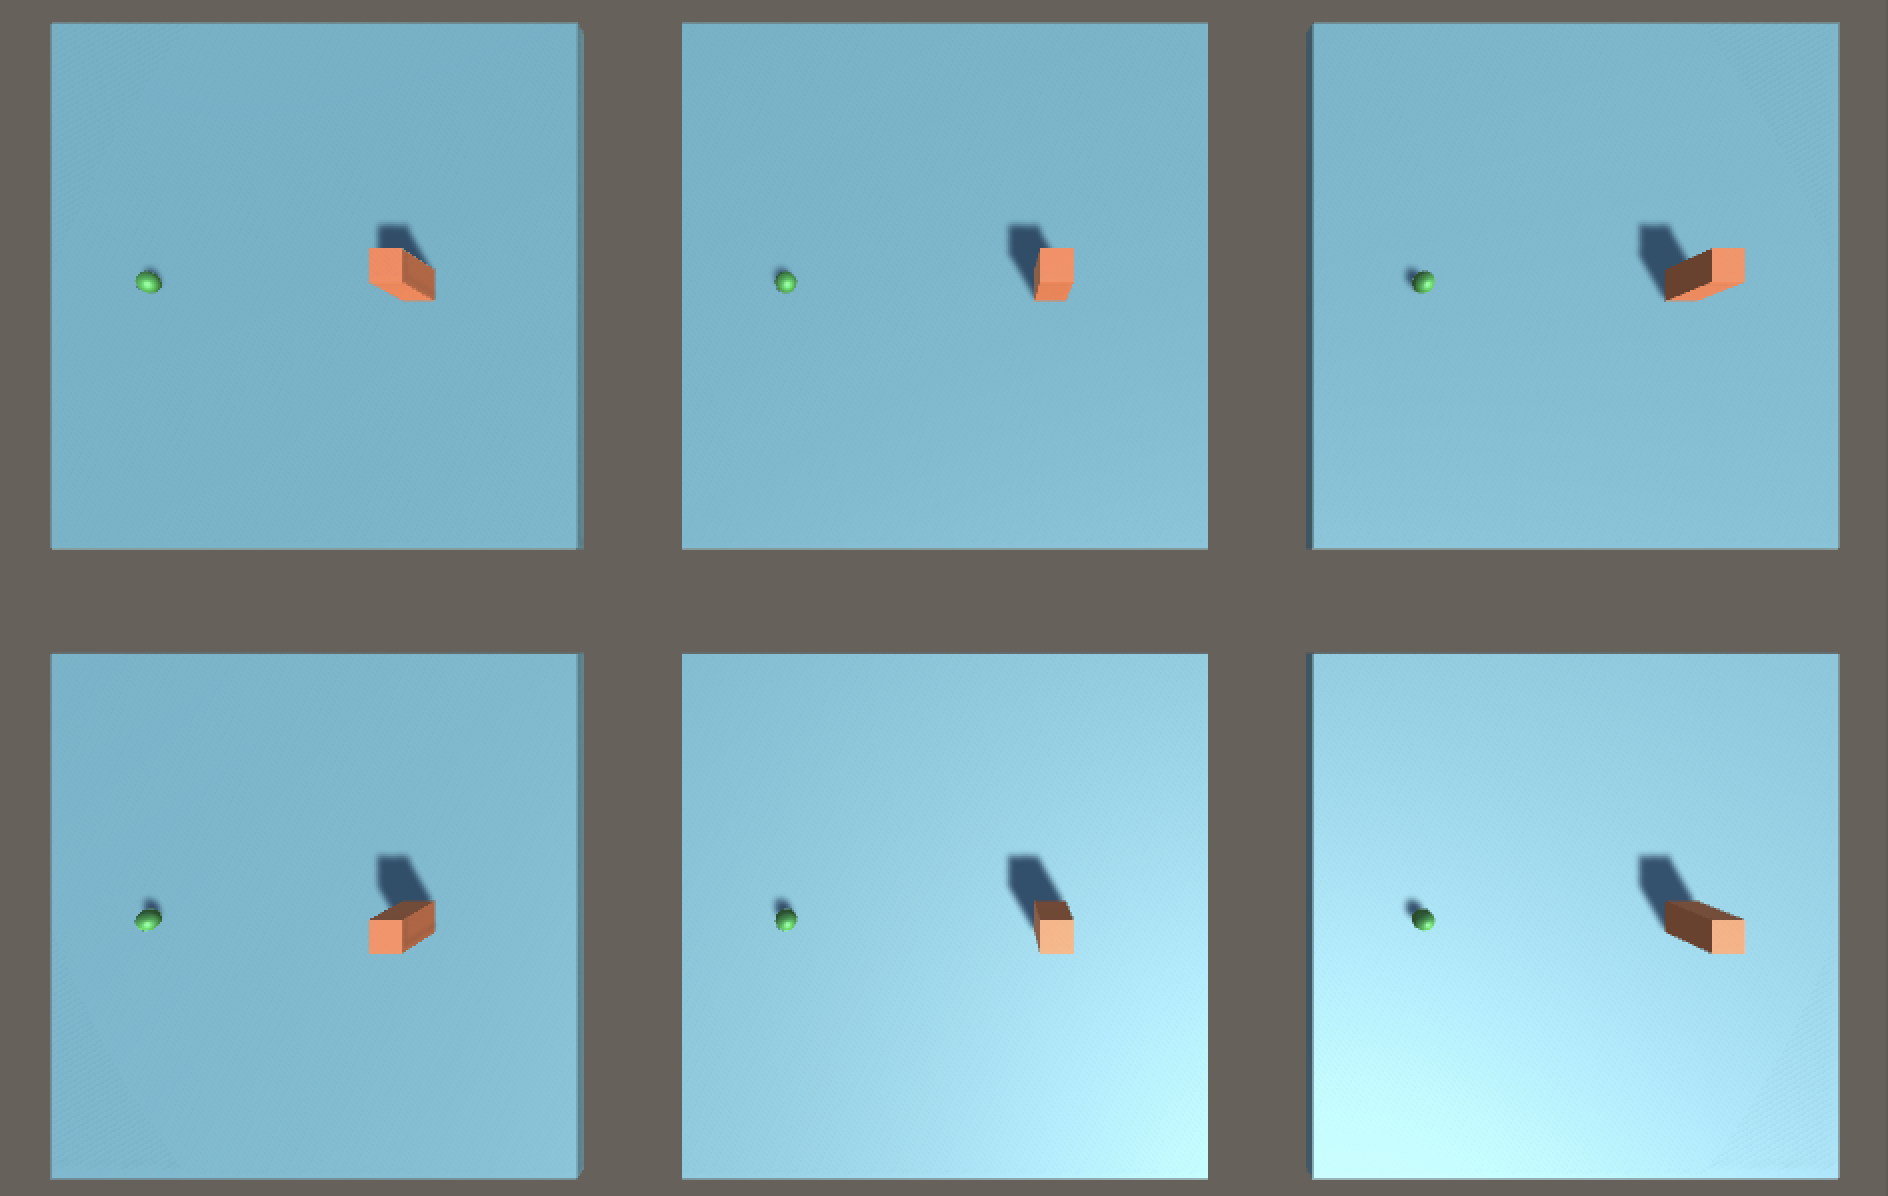
\includegraphics[scale=0.4]{images/ml-agents/example_scene_multi.png}
\caption{ML-Agents-Beispiel, aktualisierter Aufbau der Szene mit Multi-Agent-Setup}
\label{fig:ml-agents_example_scene_multi}
\end{figure}


\subsection{Training}
Das Training wurde mit \ac{ppo} und den Default-Hyperparametern durchgeführt, die um grob geschätzte Parameter erweitert wurden, die in der folgenden Auflistung zu finden sind. Die Funktionsweisen der einzelnen Hyperparameter werden im Abschnitt \ref{village_training_hyperparameter} ausführlich erläutert.

\begin{itemize}
    \item epsilon: 0.2, lambd: 0.95, beta: 3e-3, learning\_rate: 1e-3,
    \item num\_epoch: 3, max\_steps: 2e6
    \item use\_recurrent: false
    \item batch\_size: 1024, buffer\_size: 4096, time\_horizon: 32
    \item hidden\_units: 64, num\_layers: 2
    \item reward\_signals: extrinsic, strength: 1.0, gamma:0.99
\end{itemize}

Bei einem maximalen mathematisch möglichen Reward von $r = 1.0$ ergab sich bereits nach ca. 30.000 Schritten eine durchschnittliche Belohnung von $r = 0.94$ pro Episode. Nach etwa 45.000 Schritten wurde ein Wert von $r = 0.98$ erreicht und somit eine schnelle Konvergenz erreicht. Obwohl die Hyperparameter nur grob festgelegt wurden, wurde für diese einfache Aufgabe also nach kurzer Zeit ein gutes Ergebnis erzielt. Bezogen auf die kumulative Belohnung hat sich folgender Trainingsverlauf ergeben:

\begin{figure}[H]
\centering
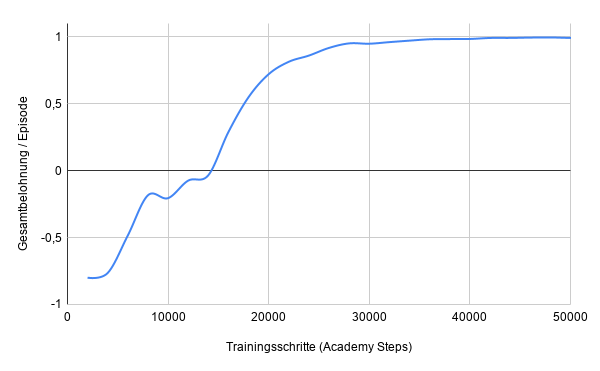
\includegraphics[scale=0.7]{images/ml-agents/diagram_example_training.png}
\caption{ML-Agents-Beispiel, kumulative Belohnung des Trainingsverlaufs}
\label{fig:ml-agents_example_training}
\end{figure}

In diesem Kapitel wurde bewiesen, dass einfache Vorgänge innerhalb kürzester Zeit gelernt werden können und dabei hohe Erfolgsquoten erreicht werden.
Im Folgenden wird auf dieser Erkenntnis aufgebaut und mit komplexeren Sachverhalten konfrontiert.
\chapter{Entwicklung bedürfnisbasierter Agenten durch Reinforcement Learning}\label{entwicklung_dorf}
Dieses Kapitel bildet den Hauptteil der Thesis und stellt den entwickelten Ansatz einer Dorfsimulation vor. Im Detail wird die Entwicklung eines Verfahrens zur Erschaffung glaubwürdiger Agenten mithilfe von Machine Learning als Alternative zur Nutzung klassischer Methoden wie Decision Trees oder Finite State Machines vorgestellt. Dazu gehöret die Entwicklung eines Prototypen für ein in Unity entwickeltes Dorfsystem, in dem sich die Agenten aufhalten. Konkret werden dafür bedürfnisbasierte Utility-Agenten verwendet, die durch Reinforcement Learning ein authentisches Verhalten erlernen sollen.
Für die Umsetzung wurde \Fachbegriff{Unity Pro} in der Version \Fachbegriff{2019.2.8f1} verwendet. Sämtlicher Code wurde in \Fachbegriff{Visual Studio} erstellt. Als Basis-Framework dient ML-Agents (siehe Kapitel \ref{ml_unity}). Für die Nutzung von Multithreading wurde weiterhin die Bibliothek \Fachbegriff{Thread Ninja} verwendet \cite{ninja}. Zunächst werden Anforderungen an die Implementierung gestellt.


\section{Anforderungen}
Es soll eine Dorfsimulation angefertigt werden, in der es Gebäude mit unterschiedlichen Zwecken gibt (beispielsweise eine Taverne, einen Marktplatz, einen Bäcker, etc.). Weiterhin soll es intelligente Bewohner geben, die in und außerhalb von Gebäuden Tätigkeiten durchführen können.
Folgende Ziele sollen bezüglich des Dorfes erfüllt werden:

\begin{itemize}
    \item \texttt{Dorf}: Es soll ein Dorfsystem entwickelt werden, in dem begehbare Gebäude mit bestimmter Kapazität und unterschiedlichen Zwecken vorhanden sind (z.B. Bäcker, Taverne, Wohnhäuser, Marktplatz, etc.). Die Simulation soll einen zeitlichen Tagesablauf mit visuellen Hinweisen wie Belichtung, Sonnenverlauf und Lichtquellen haben.
    \item \texttt{NPCs}: Das Dorf soll von NPCs bevölkert werden, die verschiedene Aktionen ausführen können. Dazu gehören Aktionen wie beispielsweise Arbeiten, Essen oder Schlafen. Jede Aktion hat ein oder mehrere Ziele, die einem Gebäudetypen entsprechen. Die Agenten müssen in der Lage sein, zu den Zielen zu navigieren. Die Aktion \textit{Schlafen} hätte beispielsweise das Wohnhaus des Agenten zum Ziel, die Aktion \textit{zur Kirche gehen} dagegen die Kirche. Aktionen können weiterhin Ressourcen produzieren oder verbrauchen.
    \item \texttt{Bedürfnisse}: Die NPCs verfügen über Bedürfniswerte, die für die Auswahl von Aktionen relevant sind. Dazu gehören menschliche Bedürfnisse wie Hunger, Schlaf, Kommunikation, Bildung, etc.
    \item \texttt{Authentisches Verhalten}: Die NPCs sollen selbstständig ein authentisches Verhalten erlernen, das vom internen Zustand der Agenten abhängt. Die Bedürfniswerte  bilden die Grundlage für die Auswahl von Aktionen. Die Bedürfnisse sollen so angepasst werden, dass sie in etwa den menschlichen Äquivalenten entsprechen. Wenn ein Agent hungrig ist, soll er automatisch die Aktion \textit{Essen} wählen. Idealerweise soll ein sinnvoller Tagesablauf abgebildet werden.
\end{itemize}



\subsection{Trennung von Modell, Darstellung und Logik}
Klassischerweise wird in der Softwareentwicklung versucht, die Darstellungsebene von der Logikebene und der Modell- bzw. Datenebene zu trennen. Häufig wird dafür das \ac{mvc}-Pattern verwendet. Dieses Vorgehen ist grundsätzlich auch in Unity anwendbar. Aufgrund der grafischen Natur einer Game Engine sowie dem grundlegenden Konzept der Verwendung von \Fachbegriff{GameObjects} (siehe Kapitel \ref{ml_unity}) findet allerdings eine größere Vermischung von Logik und Darstellung statt. In der entwickelten Anwendung werden keine Pattern wie \ac{mvc} verwendet, da hierdurch ein zu großer Overhead entstehen würde. Dieser Aufwand wäre für die Implementierung der Dorfsimulation nicht gerechtfertigt. Das Hauptziel ist nicht die Erschaffung einer gut erweiterbaren Anwendung, sondern eine Demonstration für die Möglichkeiten von Reinforcement Learning und bedürfnisbasierten Agenten. Eine Vermengung der Darstellungsebene, Logikebene und Modellebene wird akzeptiert. Es gibt daher Klassen, in denen keine klare Trennung zwischen Visualisierung und Verhalten vorgenommen wird.


\section{Modellierung}
An die in der Stadt verwendeten Gebäude wird die Anforderung gestellt, dass sie begehbar sein müssen. Da keine fertigen Assets für begehbare Gebäude zur Verfügung standen, wurde für die Modellierung des Dorfes eine externe Sammlung von modularen Assets aus dem Unity Asset Store bezogen \cite{village_modular_asset_pack}. Diese beinhaltet Texturen, Oberflächenmaterialien, Polygonnetze und Unity-Prefabs.
Mithilfe dieser Sammlung wurden eigene Gebäude aus Einzelkomponenten wie Fenstern, Wandelementen und Dekorationen angefertigt. Der Großteil der Gebäude wurde also manuell modelliert. Dadurch wird sowohl die Begehbarkeit der Gebäude sichergestellt, als auch eine höhere Modularität sowie einer Verbesserung der visuellen Attraktivität des Dorfes gewährleistet.

\begin{figure}[H]
\centering
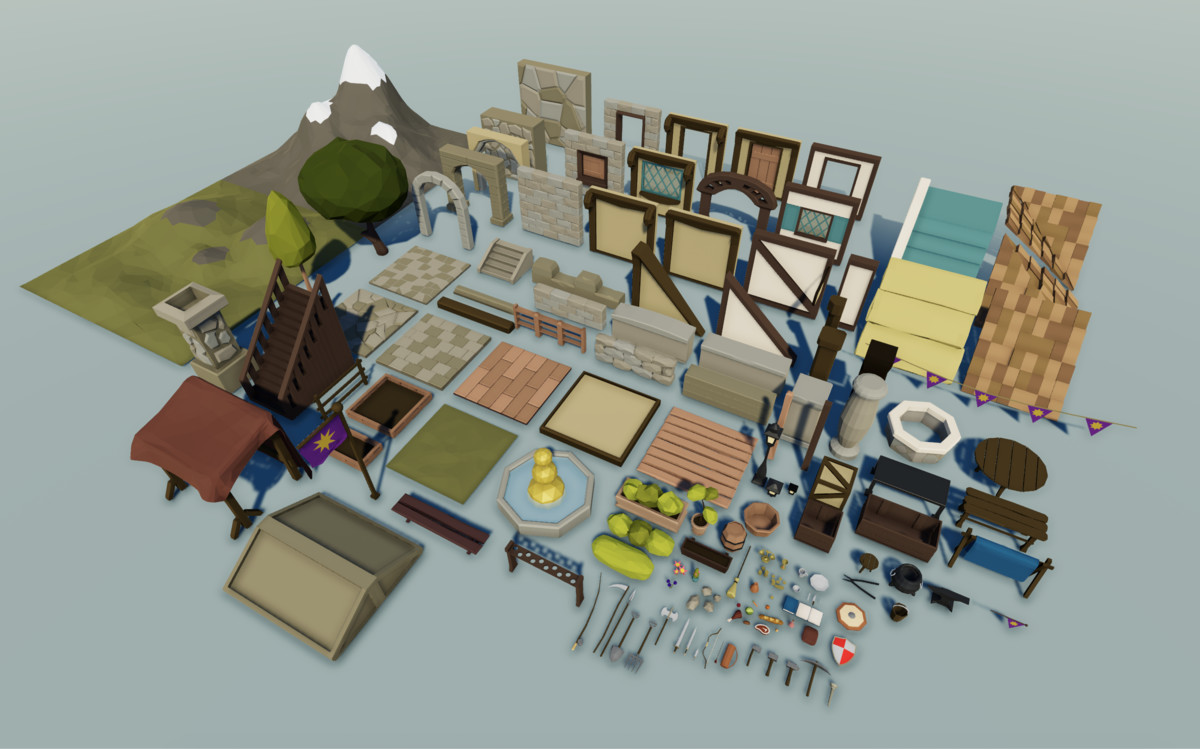
\includegraphics[scale=0.6]{images/village/modular_model_examples.jpg}
\caption{Beispiele für modulare Komponenten zur Modellierung des Dorfes}
\label{fig:modular_model_examples}
\end{figure}

Abbildung \ref{fig:modular_model_examples} zeigt einige Beispiele für modulare Komponenten. Weiterhin ist in Abbildung \ref{fig:modular_house_model_1} ein beispielhaftes Haus zu sehen, das für den Bau des Dorfes aus diesen Komponenten gebildet wurde.

\begin{figure}[H]
\centering
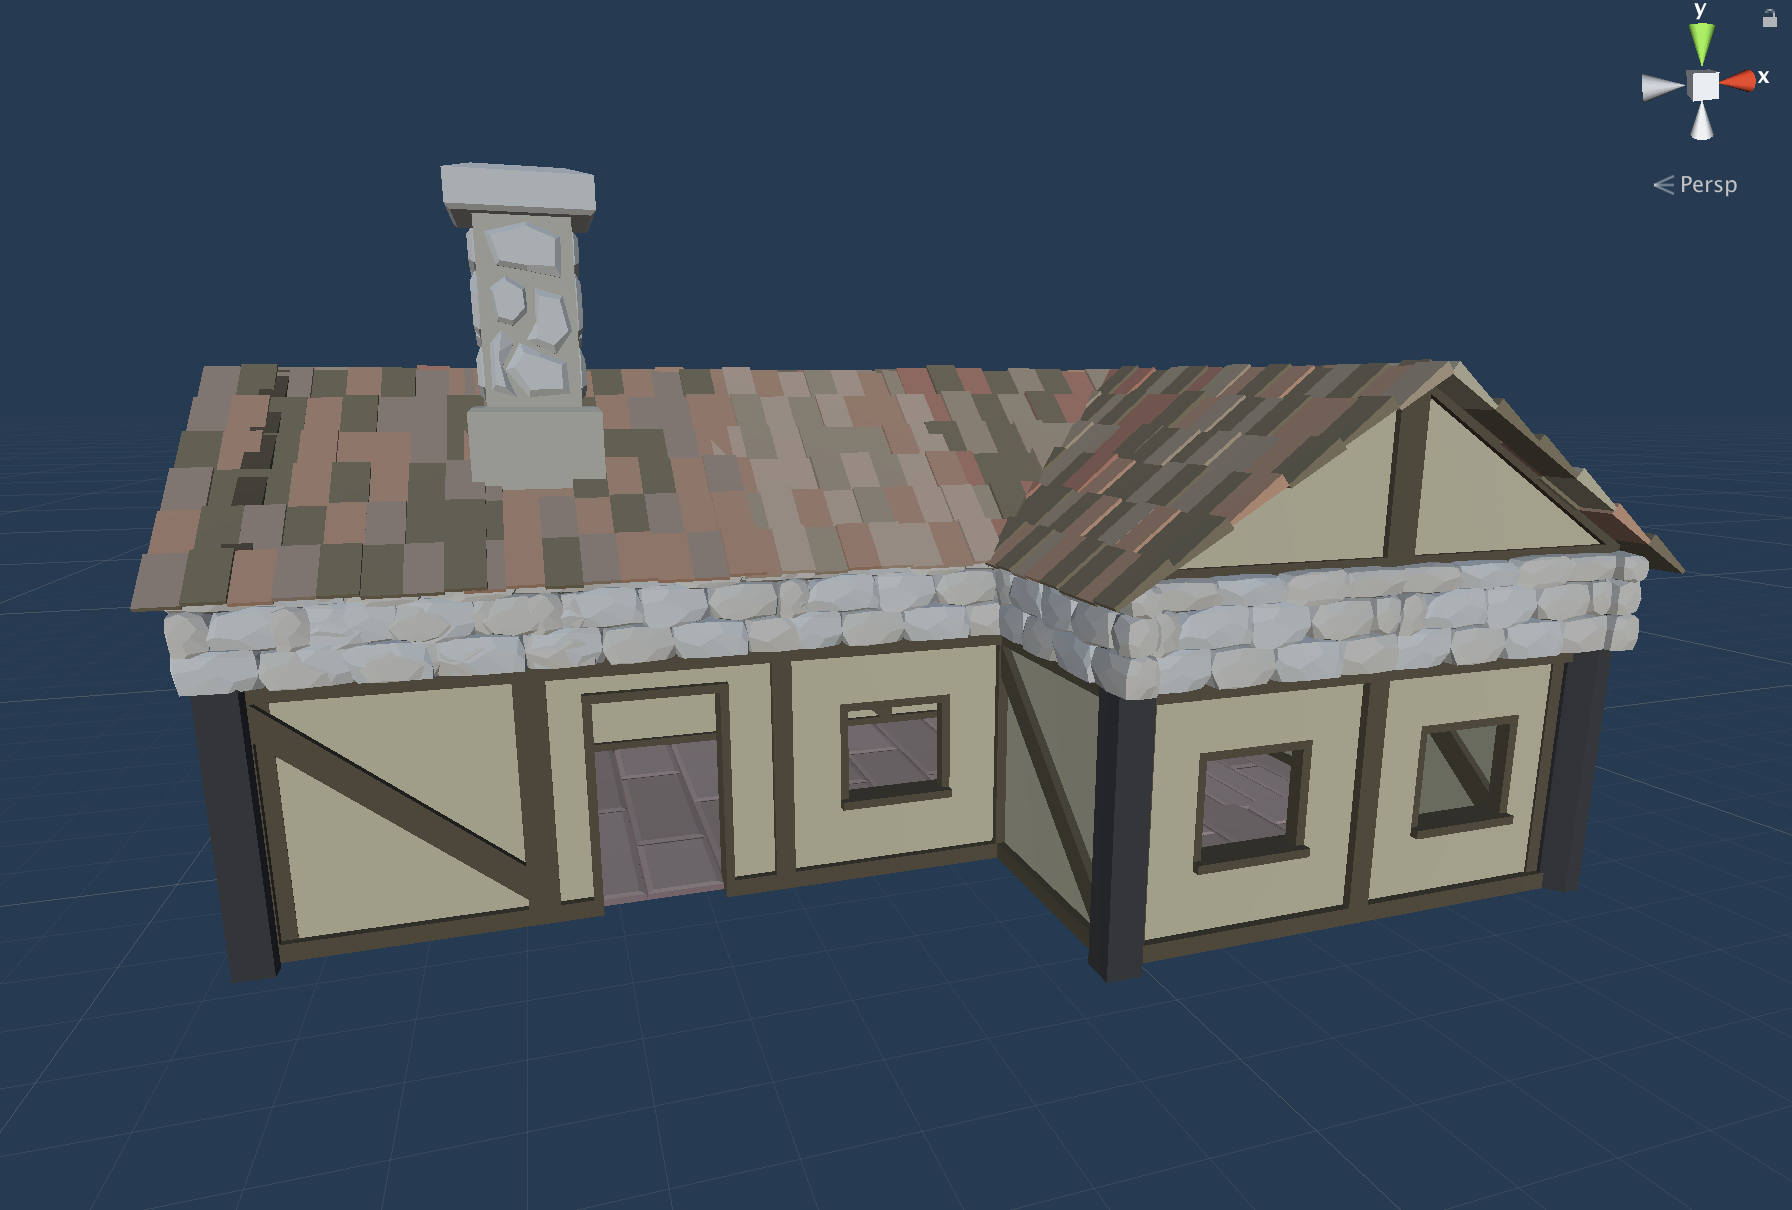
\includegraphics[scale=0.4]{images/village/modular_house_model_1.png}
\caption{Modelliertes modulares Haus}
\label{fig:modular_house_model_1}
\end{figure}

Für Dekorationen, Bäume und Weiteres wurden zusätzlich weitere Sammlungen von Assets verwendet \cite{village_campfire_asset} \cite{village_free_trees_assets} \cite{village_windmill_asset} \cite{village_citypack_asset}.

Die Abbildungen \ref{fig:village_village_day_1} und \ref{fig:village_village_day_2} zeigen die modellierte Stadt mit einer Vielzahl von Gebäuden und Dekorationen wie Bäumen und Zäunen. Auf den Abbildungen sind sowohl eine Außenansicht eines großen Teils der Stadt als auch eine beispielhafte Innenansicht einer Straße zu erkennen. Um eine visuelle Abgrenzung zur Außenwelt vorzunehmen, wurden Felsen um die Stadt herum positioniert, die nicht passierbar sind.

\begin{figure}[H]
\centering
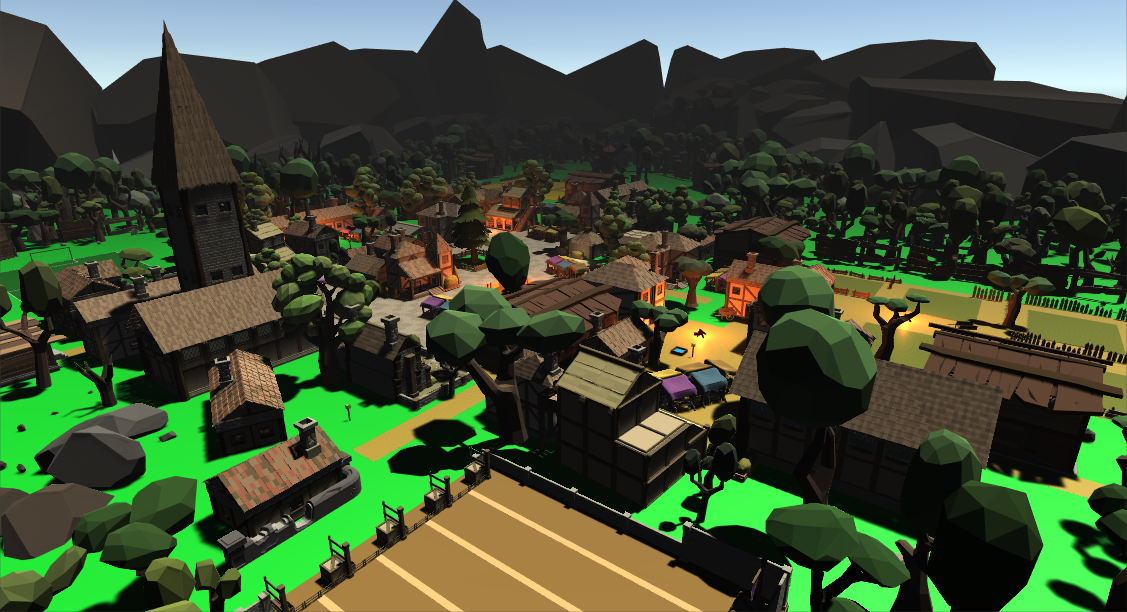
\includegraphics[scale=0.525]{images/village/village_village_day_1.PNG}
\caption{Modellierte Stadt, äußere Ansicht}
\label{fig:village_village_day_1}
\end{figure}

\begin{figure}[H]
\centering
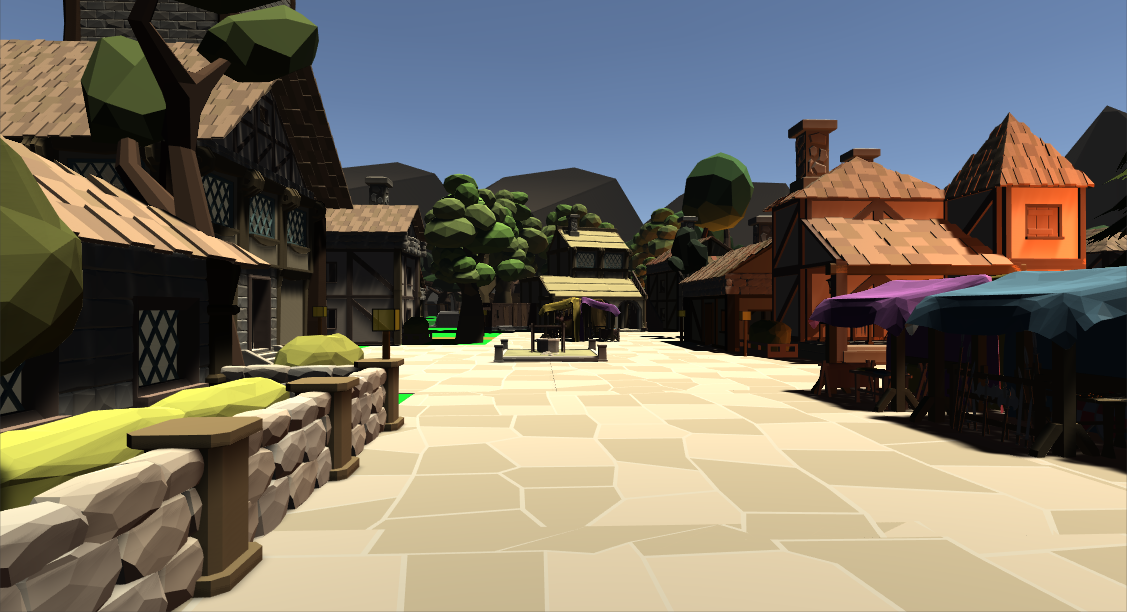
\includegraphics[scale=0.525]{images/village/village_village_day_2.png}
\caption{Modellierte Stadt, innere Ansicht}
\label{fig:village_village_day_2}
\end{figure}
















\section{Softwaredesign- und Architektur}
Im Verlauf dieses Abschnitts wird die Architektur der Simulation erläutert. Zunächst wird hierfür ein genereller Überblick vermittelt, der die grundsätzliche Struktur beschreibt. Anschließend werden die einzelnen Komponenten anhand der zentralen Klassen näher betrachtet und ihre Funktionsweise erläutert. Generell wurde ein objektorientierter Ansatz gewählt. Im Folgenden wird die in Abbildung \ref{fig:architecture_diagram_init_example} verwendete Notation verwendet, um den Aufbau von Klassen anhand der Signaturen ihrer Methoden und Felder zu beschreiben.

\begin{figure}[H]
\centering
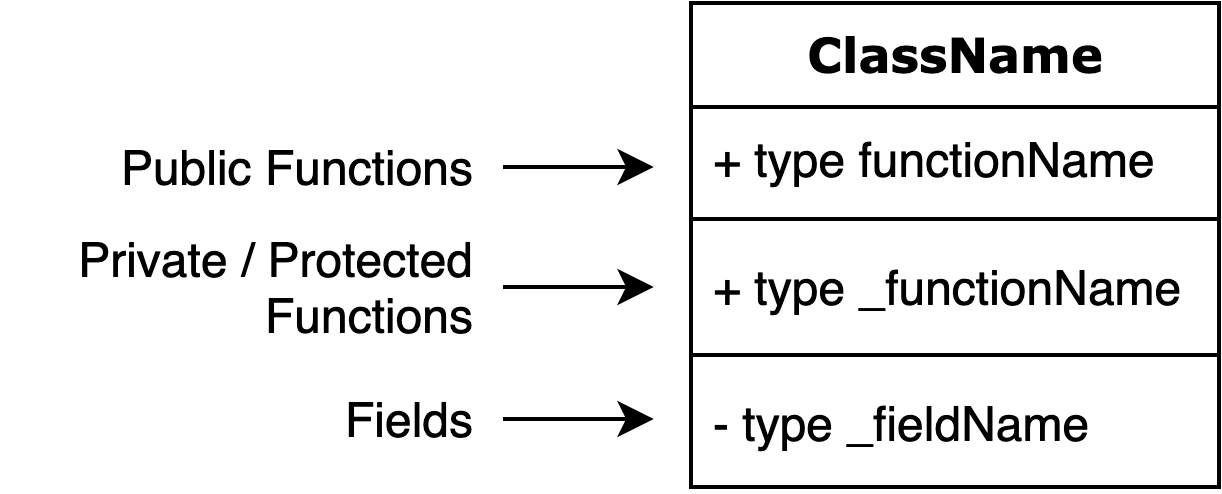
\includegraphics[scale=0.21]{images/village/architecture_diagram_init_example.png}
\caption{Verwendete Notation für die Beschreibung von Klassen}
\label{fig:architecture_diagram_init_example}
\end{figure}

Da das ML-Agents Toolkit verwendet wird, hängt die grundlegende Architektur des Dorfes teilweise von der im Kapitel \ref{ml_unity} erläuterten Struktur ab (siehe \ref{fig:ml-agents_architecture}). Insbesondere betrifft das die Entwicklung der Agenten und Entscheidungen sowie die Ausführung von Aktionen. Daher wird der in Kapitel \ref{ml_unity} vorgestellte Prozess verwendet, der eine \inlinecode{Academy}-Instanz mit mehreren Agenten und bestimmten nötigen Funktionen vorsieht.

\bigskip
\begin{figure}[H]
\centering
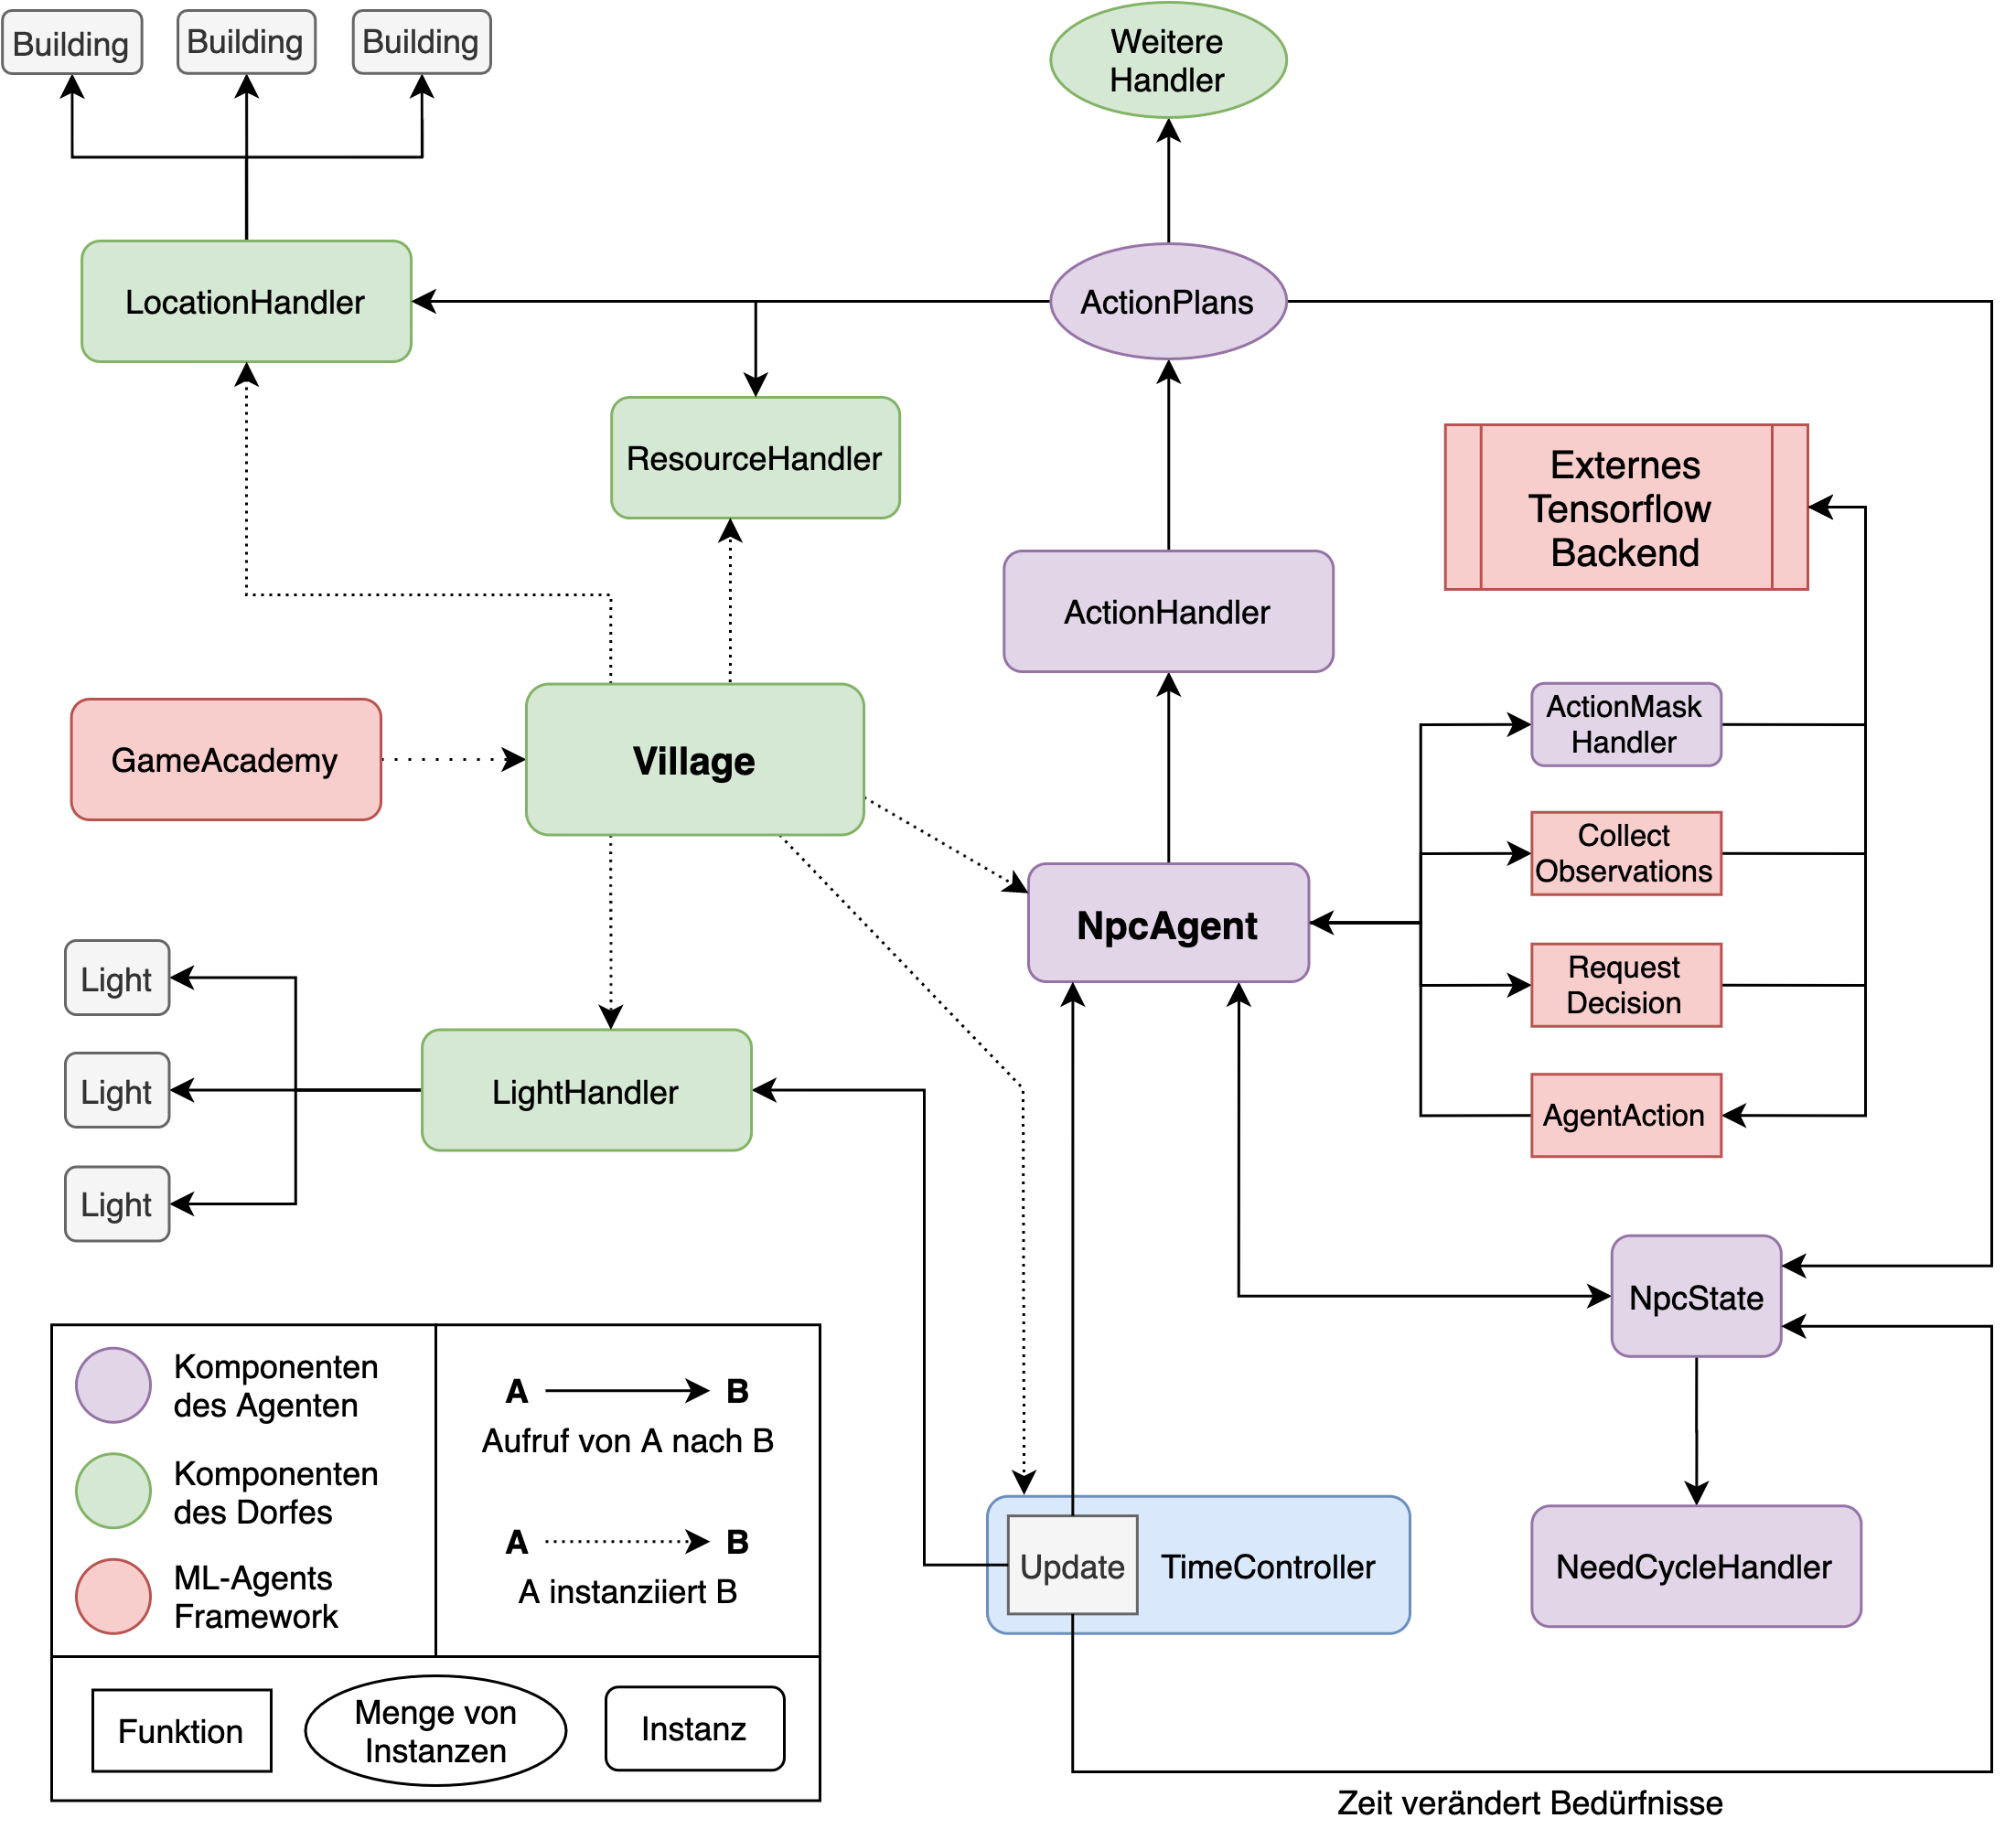
\includegraphics[scale=0.21]{images/village/Master-Thesis_Diagram_Architecture_2.png}
\caption{Grundsätzliche Architektur des Dorfsystems}
\label{fig:architecture_general}
\end{figure}

Abbildung \ref{fig:architecture_general} zeigt den grundsätzlichen Aufbau der Implementierung. Die beiden Komponenten \inlinecode{Village} und \inlinecode{NpcAgent} bilden die zentralen Elemente für den Ausführungskreislauf bzw. \Fachbegriff{Game Loop} der Simulation. Es besteht eine direkte Anbindung zum ML-Agents Toolkit über die \inlinecode{GameAcademy}. Zunächst wird \inlinecode{Village} durch die \inlinecode{GameAcademy} initialisiert. \inlinecode{Village} wiederum erzeugt eine festgelegte Anzahl von Agenten. Es gibt also eine kaskadierte Hierarchie für die Initialisierung der Simulation mit der \inlinecode{GameAcademy} an höchster Stelle, gefolgt von mehreren Instanzen vom Typ \inlinecode{Village} und schließlich jeweils mehreren Instanzen vom Typ \inlinecode{NpcAgent}.

\inlinecode{Village} verfügt über verschiedene Subkomponenten, die für das Steuern bestimmter Aufgaben verantwortlich sind. Über den \inlinecode{ResourceHandler} wird das Ressourcensystem verwaltet, auf das die NPCs zugreifen können. Zusätzlich verwaltet der \inlinecode{LocationHandler} alle Orte im Spiel, zu denen ein Agent navigieren kann. Dazu gehören sämtliche Häuser inklusive deren Räume und weitere Orte außerhalb von Gebäuden. Zuletzt ist der \inlinecode{LightHandler} dafür zuständig, die Tageszeit anhand des Sonnenstandes und der Kontrolle von Lichtquellen zu simulieren.
Der \inlinecode{NpcAgent} erbt von der ML-Agents-Klasse \inlinecode{Agent} und ist somit für das Reinforcement Learning und die Ausführung von Aktionen vorhanden. Das Framework wählt Aktionen für den Agenten aus und stößt diese an. Die Aktionen, die ein Agent ausführen kann, benötigen immer ein Ziel und verwenden daher den \inlinecode{LocationHandler}. Sie beeinflussen außerdem den Zustand \inlinecode{NpcState} eines Agenten. Dieser beinhaltet beispielsweise die Bedürfnisse eines Agenten, die von Aktionen aufgefüllt werden können. Die Funktionen, die die Abnahme der Bedürfnisse bestimmen, werden im \inlinecode{NeedCycleHandler} definiert und werden über diesen aktualisiert. Aktionen können außerdem Ressourcen aufbrauchen oder produzieren, indem der \inlinecode{ResourceHandler} verwendet wird.

Eine zentrale Zeitverwaltungseinheit wird durch den \inlinecode{TimeController} realisiert. Dieser berechnet in regelmäßigen Abständen aufgrund der verstrichenen Zeit die neue Zeit im Spiel. Anschließend werden alle Komponenten, für die das Voranschreiten der Zeit relevant ist, mit dieser neuen Zeit versorgt. Der \inlinecode{LightHandler} regelt mit dessen Hilfe beispielsweise die Intensität und Position der Sonne wohingegen der \inlinecode{NeedCycleHandler} aufgrund der verstrichenen Zeit die neuen Bedürfnisse des Agenten berechnet und den \inlinecode{NpcState} entsprechend anpasst.



\section{Implementierung}
In den folgenden Abschnitten werden die wichtigsten Klassen der Dorfsimulation im Einzelnen erläutert. Zunächst werden dafür die zentralen, übergeordneten Komponenten \inlinecode{Village} und \inlinecode{GameAcademy} näher betrachtet.


\subsection{Village}
Die Aufgabe der Komponente \inlinecode{Village} ist die Erzeugung von \acp{npc} und die Bereitstellung einer zentralen Verwaltungseinheit für Komponenten. Abbildung \ref{fig:architecture_diagram_village} zeigt den Aufbau der Klasse \inlinecode{Village} anhand ihrer Funktionen:

\begin{figure}[H]
\centering
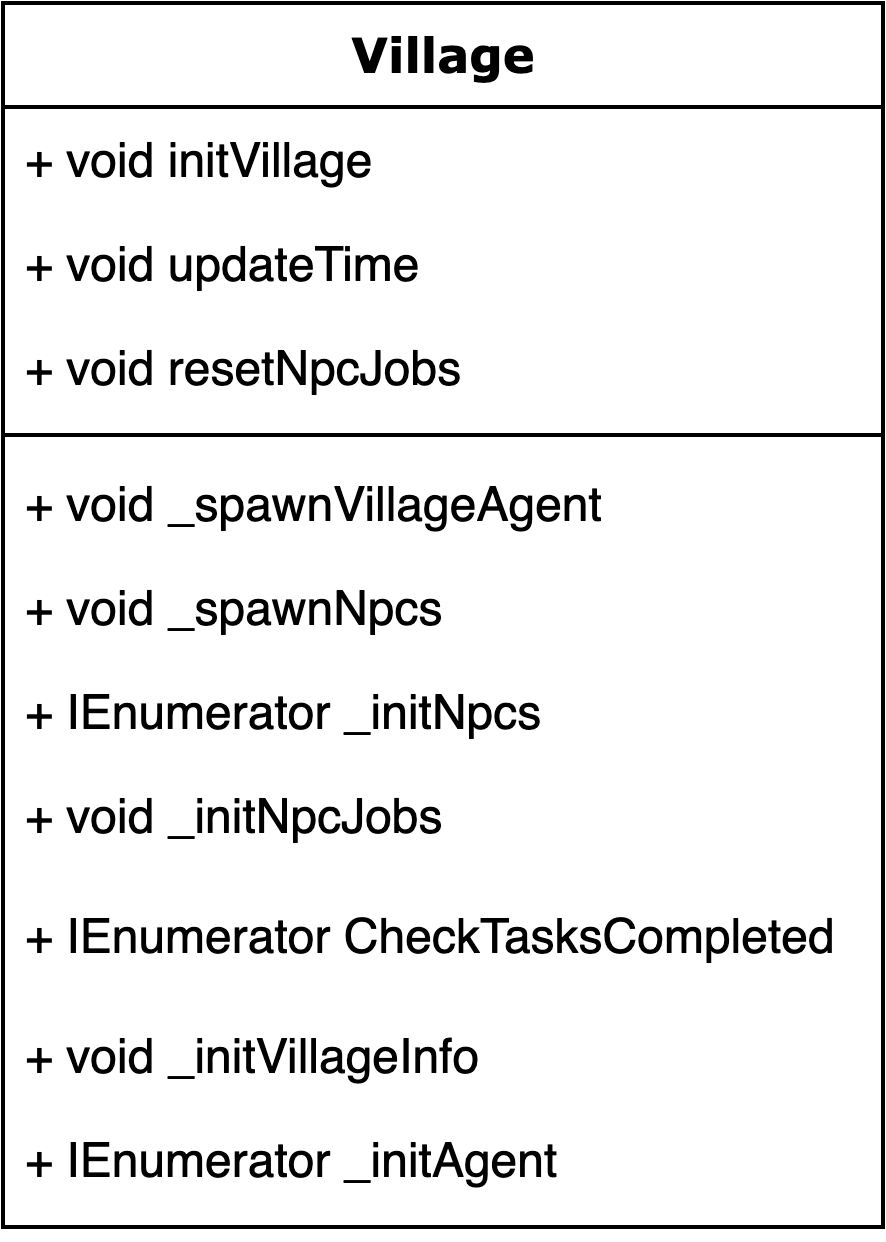
\includegraphics[scale=0.18]{images/village/architecture_diagram_village.png}
\caption{Methoden der Klasse \inlinecode{Village}}
\label{fig:architecture_diagram_village}
\end{figure}

\inlinecode{Village} erzeugt und initialisiert zunächst Handler-Klassen wie \inlinecode{TimeController}, \inlinecode{LocationHandler}, \inlinecode{ResourceHandler} und \inlinecode{LightHandler} in der Funktion \inlinecode{initVillage}. Anschließend werden weitere Funktionen aufgerufen, um innerhalb von Coroutinen asynchron Agenten zu erzeugen. Diese werden in \inlinecode{\_spawnNpcs} zunächst erstellt und dann in \inlinecode{\_initNpcs} initialisiert, wie in Listing \ref{lst:village_init_npcs} zu sehen.

\begin{minipage}{\linewidth}
\begin{lstlisting}[linewidth=16.4cm, label=lst:village_init_npcs, caption=Initialisierung von Agenten, xleftmargin=1cm]
private IEnumerator _initNpcs() {
    _npcLoadingTasks = new Dictionary<int, bool>();
    for (int i = 0; i < _villageNpcs.Count; i++) {
        _npcLoadingTasks[i] = false;
        _villageNpcs[i].StartCoroutine(_initAgent(i));
    }
    yield return StartCoroutine(CheckTasksCompleted());
    _villageAgent.init(this);
    GameAcademy.NPC_LOADING_DONE = true;
}
\end{lstlisting}
\end{minipage}

Für jeden Agenten wird eine einzelne Coroutine \inlinecode{\_initAgent} gestartet. Anschließend wird mit \inlinecode{yield return} auf die Ausführung einer weiteren Coroutine \inlinecode{CheckTasksCompleted} gewartet, die in bestimmten Abständen prüft, ob die weiteren Coroutinen beendet wurden.

Mit der Funktion \inlinecode{\_spawnVillageAgent} wird darüber hinaus die Klasse \inlinecode{VillageAgent} initialisiert (siehe Abschnitt \ref{village_village_agent}). Sobald alle \inlinecode{NpcAgent}s erfolgreich initialisiert wurden, wird auch der \inlinecode{VillageAgent} initialisiert.

\inlinecode{Village} speichert Referenzen auf alle Agenten \inlinecode{NpcAgent} des Dorfes und bietet eine Schnittstelle für weitere Komponenten, um Zugriff auf die Agenten zu erlangen. Zusätzlich verfügt das Dorf über eine Instanz der Klasse \inlinecode{VillageInfo}, die in der Methode \inlinecode{\_initVillageInfo} erzeugt wird. Darin werden Informationen über den aktuellen Zustand des Dorfes gespeichert. Dazu gehört beispielsweise die Anzahl der Agenten, die aktuell eine bestimmte Aktion ausführen. Diese Daten werden anschließend im UI der Simulation dargestellt. Aus diesem Grund verfügt \inlinecode{VillageInfo} über eine Vielzahl von Tracking-Funktionen, die diese Statistiken verwalten.




\subsection{GameAcademy}\label{gameacademy}
Die \inlinecode{GameAcademy} erbt von der ML-Agents Basisklasse \inlinecode{Academy} (siehe Kapitel \ref{ml_unity}) und erweitert diese um verschiedene Einstellungsmöglichkeiten sowie dem Ladevorgang des Dorfes. In Abbildung \ref{fig:architecture_diagram_gameacademy} wird der Aufbau der Klasse verdeutlicht:

\begin{figure}[H]
\centering
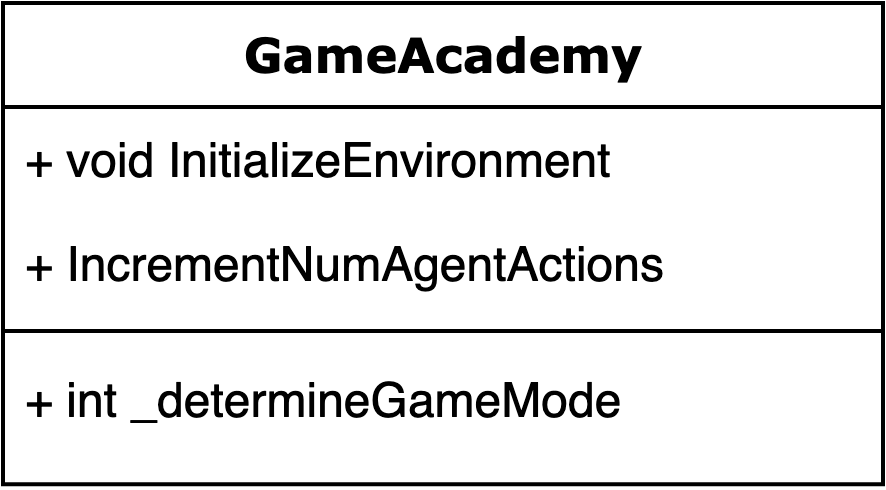
\includegraphics[scale=0.18]{images/village/architecture_diagram_gameacademy.png}
\caption{Methoden der Klasse \inlinecode{GameAcademy}}
\label{fig:architecture_diagram_gameacademy}
\end{figure}

Zunächst wird die Funktion \inlinecode{InitializeEnvironment} durch \inlinecode{ML-Agents} aufgerufen. Hier werden zunächst einige Parameter ausgewertet, die über den Unity Editor gesetzt werden können. Neben den Parametern der Oberklasse \inlinecode{Academy} können hier für die Simulation grundlegende Einstellungen vorgenommen werden, wie die Anzahl der zu erzeugenden NPCs oder die Auswahl des Inference-Modus zwischen den unterschiedlichen implementierten Verfahren wie beispielsweise Reinforcement Learning oder GOAP. Für jeden dieser Parameter existiert eine statische Variable, die von allen verwendeten Komponenten innerhalb des Dorfes einfach gelesen werden kann.
Aufgrund dieser Parameter sowie dem Rückgabewert von \inlinecode{GetIsInference} wird in der Funktion \inlinecode{\_determineGameMode} anschließend eine weitere Variable gesetzt, die den Spielmodus festlegt. Bestimmte Komponenten verhalten sich je nach Spielmodus auf eine andere Art und Weise (siehe Abschnitt \ref{modes_fake_inference_etc}).

Alle Komponente vom Typ \inlinecode{Village} werden anschließend durch die Anweisung \inlinecode{FindObjectsOfType<Village>()} hinzugefügt. Die \inlinecode{GameAcademy} startet dann den Ladevorgang der Simulation, indem alle Instanzen von \inlinecode{Village} initialisiert werden. Mehrere Dörfer mit jeweils einem \inlinecode{Village}-Modul können gleichzeitig verwendet werden, indem das Prefab für das Spielfeld dupliziert wird.

Die Funktion \inlinecode{IncrementNumAgentActions} ist ausschließlich für den \inlinecode{VillageAgent} relevant und wird im Abschnitt \ref{village_village_agent} behandelt.

Die in Tabelle \ref{tab:game_academy_parameters} zu sehenden Parameter können in der \inlinecode{GameAcademy} angepasst werden. Die Tabelle enthält für jeden Parameter eine kurze Beschreibung, die aus den entsprechenden Kommentaren im Programmcode entnommen wurden.

\smallskip
\begin{table}[H]
\footnotesize
\centering
\begin{tabular} {|  p{4.2cm}  |  p{11.4cm}  |} \hline
\textbf{Parameter} & \textbf{Beschreibung} \\ \hline

\inlinecode{numAgentsPerVillage25} & Define how many agents should be spawned per village. This should be in order of 25s (25, 50, 75...), for the jobs distribution to work properly. \\ \hline
\inlinecode{actionsPerAgentUntilReset} & Define how many decisions the agents should perform until they are reset. \\ \hline
\inlinecode{debugMode} & Tracks some additional data useful for debugging when activated. \\ \hline
\inlinecode{useFakeInference} & Since high timescale levels do not scale well with NavMeshAgents, a kind of fake inference will have to be used, in which agents teleport to their destinations and additionally wait for an amount of time that is equal to the time it would have taken to move there. \\ \hline
\inlinecode{verbose} & Prints some additional information when activated. \\ \hline
\inlinecode{actionsUntilVillageAction} & Decides how many steps will be performed per agent between VillageAgent decisions. \\ \hline
\inlinecode{villageDecisionsReset} & Decides how many decisions will be made by the VillageAgent until Done is called. \\ \hline
\inlinecode{useManualNpcDecisions} & Uses manual decisions instead of the trained model. \\ \hline
\inlinecode{ignoreVillageAgent} & Ignores the village agent and sticks with the initial distribution of jobs. \\ \hline
\inlinecode{useGoap} & Uses GOAP agents instead of a trained model. \\ \hline
\inlinecode{agentStoppingDistance} & Determines how far from his target an agent will stop when moving to a destination. \\ \hline
\inlinecode{agentRythmVariation} & Decides the amount of variation between the day/night cycles of the agents. \\ \hline
\inlinecode{logActionDurations} & Determines whether the duration of actions should be tracked in VillageInfo. \\ \hline
\inlinecode{logRewards} & Determines whether the rewards should be tracked for each action to gain some statistical information. \\ \hline
\inlinecode{logNeeds} & Logs the average needs of NPCs at certain times for later analysis. \\ \hline
\inlinecode{logAttributes} & Logs the average attributes of agents for each action. \\ \hline
\inlinecode{logActionMaskAmounts} & Determines whether to log the amount of actions that are masked respectively. \\ \hline
\inlinecode{ignoreAllResources} & Completely ignores all resource handling when set to true. \\ \hline
\inlinecode{ignoreJobMask} & Ignores the job that has been designated to an angent and instead doesn't mask jobs. \\ \hline


\end{tabular}
\caption{Konfigurierbare Parameter der \inlinecode{GameAcademy}}
\label{tab:game_academy_parameters}
\end{table}




\subsubsection{Nutzung mehrerer Villages}
Die Simulation ist nicht auf die Nutzung eines einzelnen Dorfes limitiert. Tatsächlich kann die Verwendung mehrerer Dörfer für den Trainingsvorgang vorteilhaft sein. Aus diesem Grund wurden sämtliche Komponenten so entwickelt, dass mehrere Dörfer reibungsfrei parallel betrieben werden. Zwar beeinflusst dies massiv die Performance des Testsystems, jedoch können dadurch deutlich mehr Agenten verwendet werden - bei der Verwendung eines einzelnen Dorfes würden die Kapazitäten der Gebäude sonst schnell überschritten werden. Weiterhin können dadurch Erfahrungen gesammelt werden, die diverser sind, da die Zustände der Umgebung in unterschiedlichen Dörfern voneinander abweichen.

Zur Verwendung mehrerer Dörfer muss das Prefab des Spielfeldes, das unter anderem das gesamte Mesh beinhaltet, dupliziert werden. Es ist wichtig, dass die Position des Prefabs verändert wird, damit keine Überschneidungen entstehen. Weiterhin sollten alle vorberechneten Daten wie Lichtinformationen oder das NavMesh (siehe Abschnitt \ref{agent_navigation} erneut berechnet werden.
Die \inlinecode{GameAcademy} ist unter anderem für die Initialisierung der Dörfer zuständig. Sie sucht nach allen \inlinecode{Village}-Komponenten in der gesamten Spielszene. Wie in Abbildung \ref{fig:architecture_villages_loading} erkennbar, werden die Dörfer einzeln und unabhängig voneinander geladen. Die Pfeile in der Grafik geben an, welche Klassen durch welche Komponenten instanziiert werden. Das gesamte Ökosystem eines Dorfes, inklusive der Ausführung von Aktionen, verläuft vollkommen unabhängig. Jedes Dorf stellt eine in sich gekapselte Einheit dar, die mit der Außenwelt innerhalb der Simulation, also mit anderen Dörfern, nicht kommuniziert. Jedes Dorf verfügt also über eigene Komponenten wie \inlinecode{ResourceHandler}, \inlinecode{LocationHandler} oder \inlinecode{Village}.

\bigskip
\begin{figure}[H]
\centering
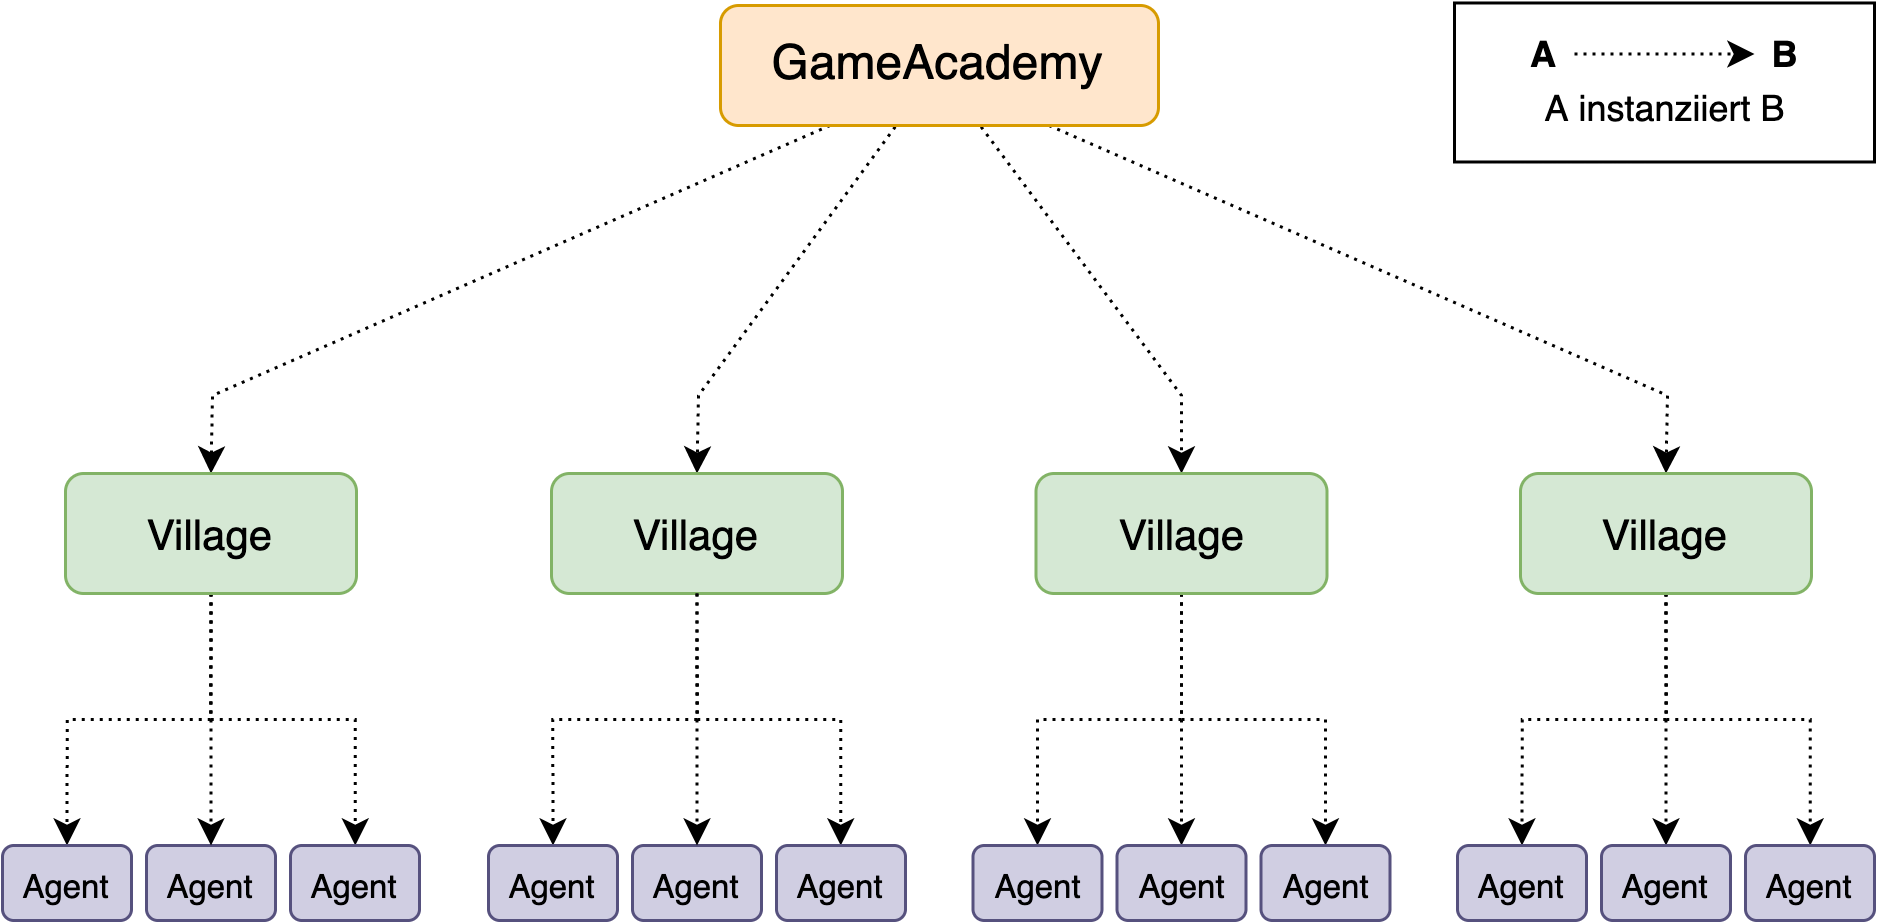
\includegraphics[scale=0.22]{images/village/Master-Thesis_Diagram_Architecture_1.png}
\caption{Architektur, Ladevorgang mehrer Dörfer}
\label{fig:architecture_villages_loading}
\end{figure}





% was verwaltet das dorf alles?

\subsection{LocationHandler}
Die Klasse \inlinecode{LocationHandler} kennt alle im Spiel verfügbaren Gebäude und Orte und bietet allen Agenten eine Schnittstelle, um mit diesen zu interagieren. Er ermöglicht somit neben der benötigten Navigation ebenfalls das Abfragen von Informationen zu bestimmten Gebäudetypen. Die Gebäude haben jeweils eine begrenzte Kapazität, es kann sich also nur eine bestimmte Anzahl von NPCs gleichzeitig in einem Haus befinden. Daher kümmert der \inlinecode{LocationHandler} sich weiterhin um die Verwaltung dieser verfügbaren \inlinecode{Slots}. Der \inlinecode{LocationHandler} wird ausdrücklich nicht für die eigentliche Navigation der Agenten verwendet, stattdessen werden lediglich Orte verwaltet und Positionen zurückgegeben.
Der \inlinecode{LocationHandler} wird durch die Klasse \inlinecode{Village} erzeugt. Abbildung \ref{fig:architecture_diagram_locationhandler} beschreibt den Aufbau.

\begin{figure}[H]
\centering
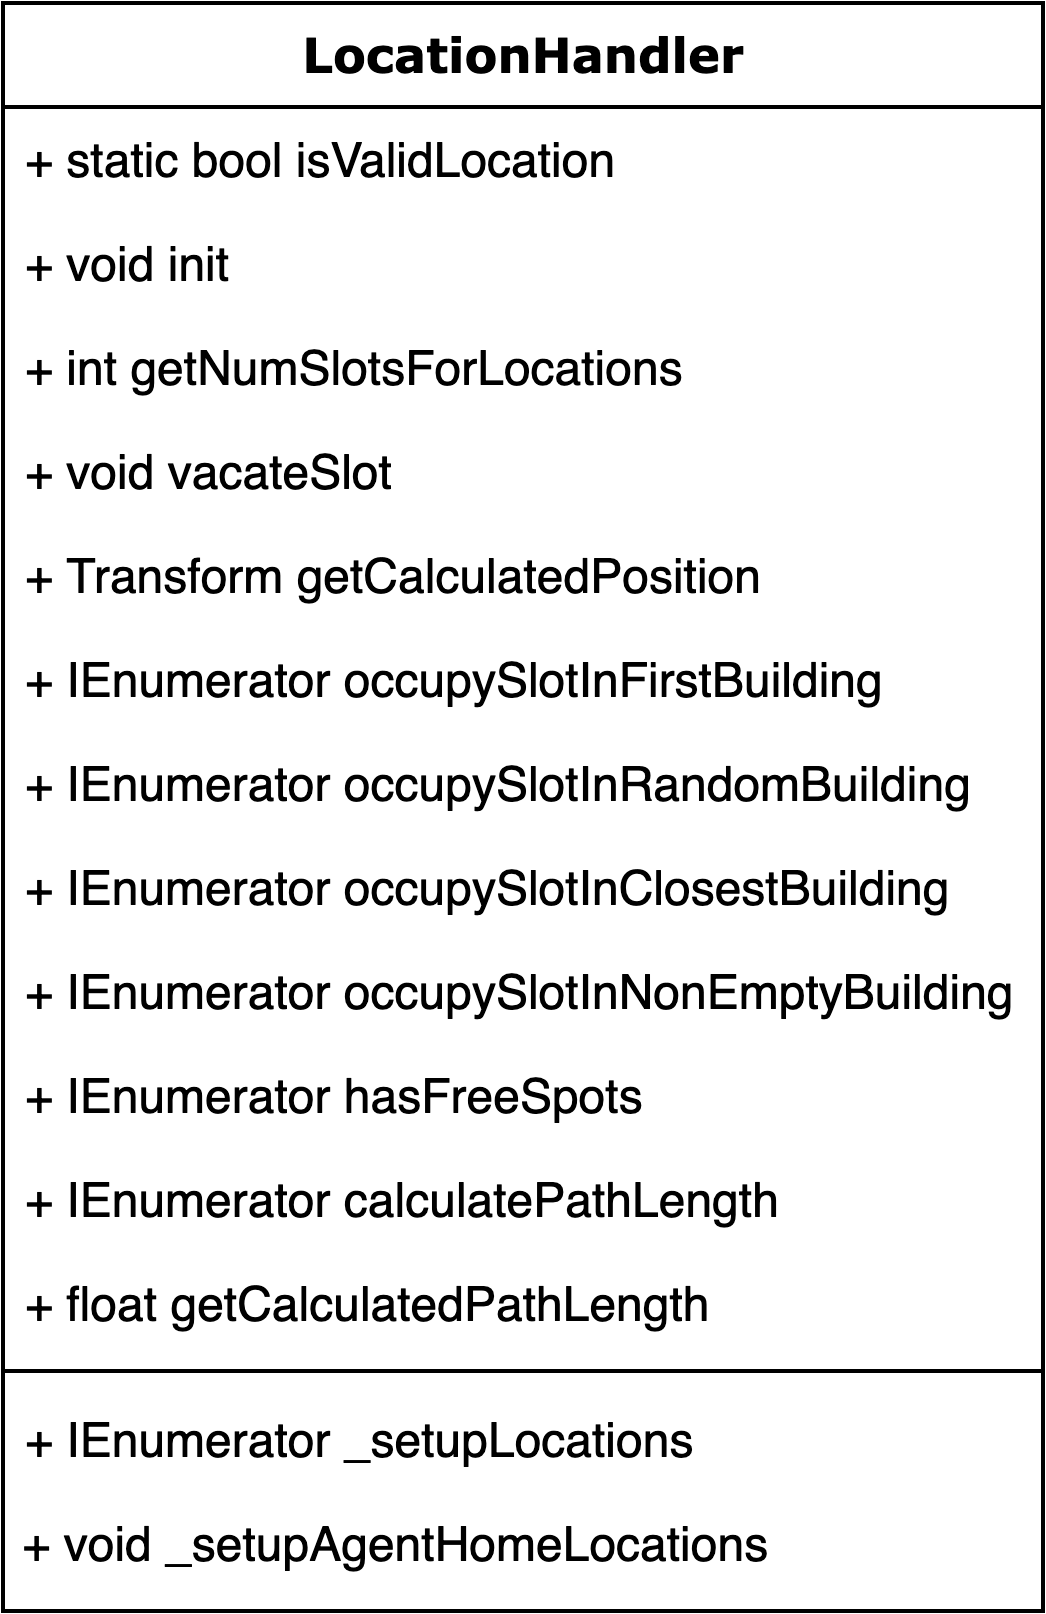
\includegraphics[scale=0.18]{images/village/architecture_diagram_locationhandler.png}
\caption{Methoden der Klasse \inlinecode{LocationHandler}}
\label{fig:architecture_diagram_locationhandler}
\end{figure}

Nach der Initialisierung durch \inlinecode{init} wird zunächst allen Agenten in der Funktion \inlinecode{\_setupAgentHomeLocations} ein Heim zugewiesen, in dem sie wohnen. In der Funktion \inlinecode{\_setupLocations} werden weiterhin alle Gebäude abhängig von ihrem Typ in einem Assoziativen Array gespeichert. in C\# wird dafür typischerweise ein \inlinecode{Dictionary} verwendet, daher ein Feld vom Typen \inlinecode{Dictionary<string, List<Building> >} genutzt. Die verschiedenen Gebäudetypen werden in der Klasse \inlinecode{LocationTypes} definiert, beispielsweise \inlinecode{FIELD\_GRAIN}, \inlinecode{BAKERY} oder \inlinecode{SCHOOL}. Diese werden als Schlüssel verwendet. Die Werte des Dictionary enthalten Listen von Gebäuden (\inlinecode{List<Building>}). Wenn der \inlinecode{LocationHandler} initialisiert wird, werden alle Gebäude des Dorfes gesucht und in die jeweilige Kategorie sortiert. Diese Suche wird beschleunigt, indem alle Gebäude mit einem Tag versehen werden.
Jedes Gebäude und jeder navigierbare Ort in der Stadt verfügt über die Komponente \inlinecode{Building}. In jedem Gebäude-Prefab werden sogenannte \inlinecode{BuildingNavPoint}s definiert, welche die tatsächlichen Orte bzw. \Fachbegriff{Slots} darstellen, zu denen die Agenten navigieren können. Dafür werden Objekte erstellt, die eine Position innerhalb des Gebäudes zugewiesen bekommen. Diesen wird die Komponente \inlinecode{BuildingNavPoint} angefügt. Die Menge der \inlinecode{BuildingNavPoint} in einem Gebäude bestimmt die Kapazität des Gebäudes. \inlinecode{BuildingNavPoint} können von nur einem NPC zur Zeit durch den Aufruf der Funktion \inlinecode{occupy} besetzt werden und müssen, sobald der Agent den Ort verlässt, anschließend durch die Funktion \inlinecode{vacate} wieder geräumt werden. Zusätzlich wird ein \inlinecode{DistanceNavPoint} definiert. Dieser wird verwendet, um die Distanz des Agenten zu einem bestimmten Gebäude zu ermitten und befindet sich daher im Eingang des Gebäudes. Falls es mehrere Eingänge gibt, wird die Mitte des Hauses gewählt. Die Abbildung \ref{fig:village_navpoints} zeigt beispielhaft, wie \inlinecode{BuildingNavPoint} und der \inlinecode{BuildingDistanceNavPoint} in einem beispielhaften Gebäude definiert werden. Zur besseren Darstellung wurde jedem \inlinecode{BuildingNavPoint} ein Mesh in Form von einer Kugel zugewiesen, die normalerweise deaktiviert ist. Für die Platzierung der Objekte kann dieses Mash aktiviert werden.

\begin{figure}[H]
\centering
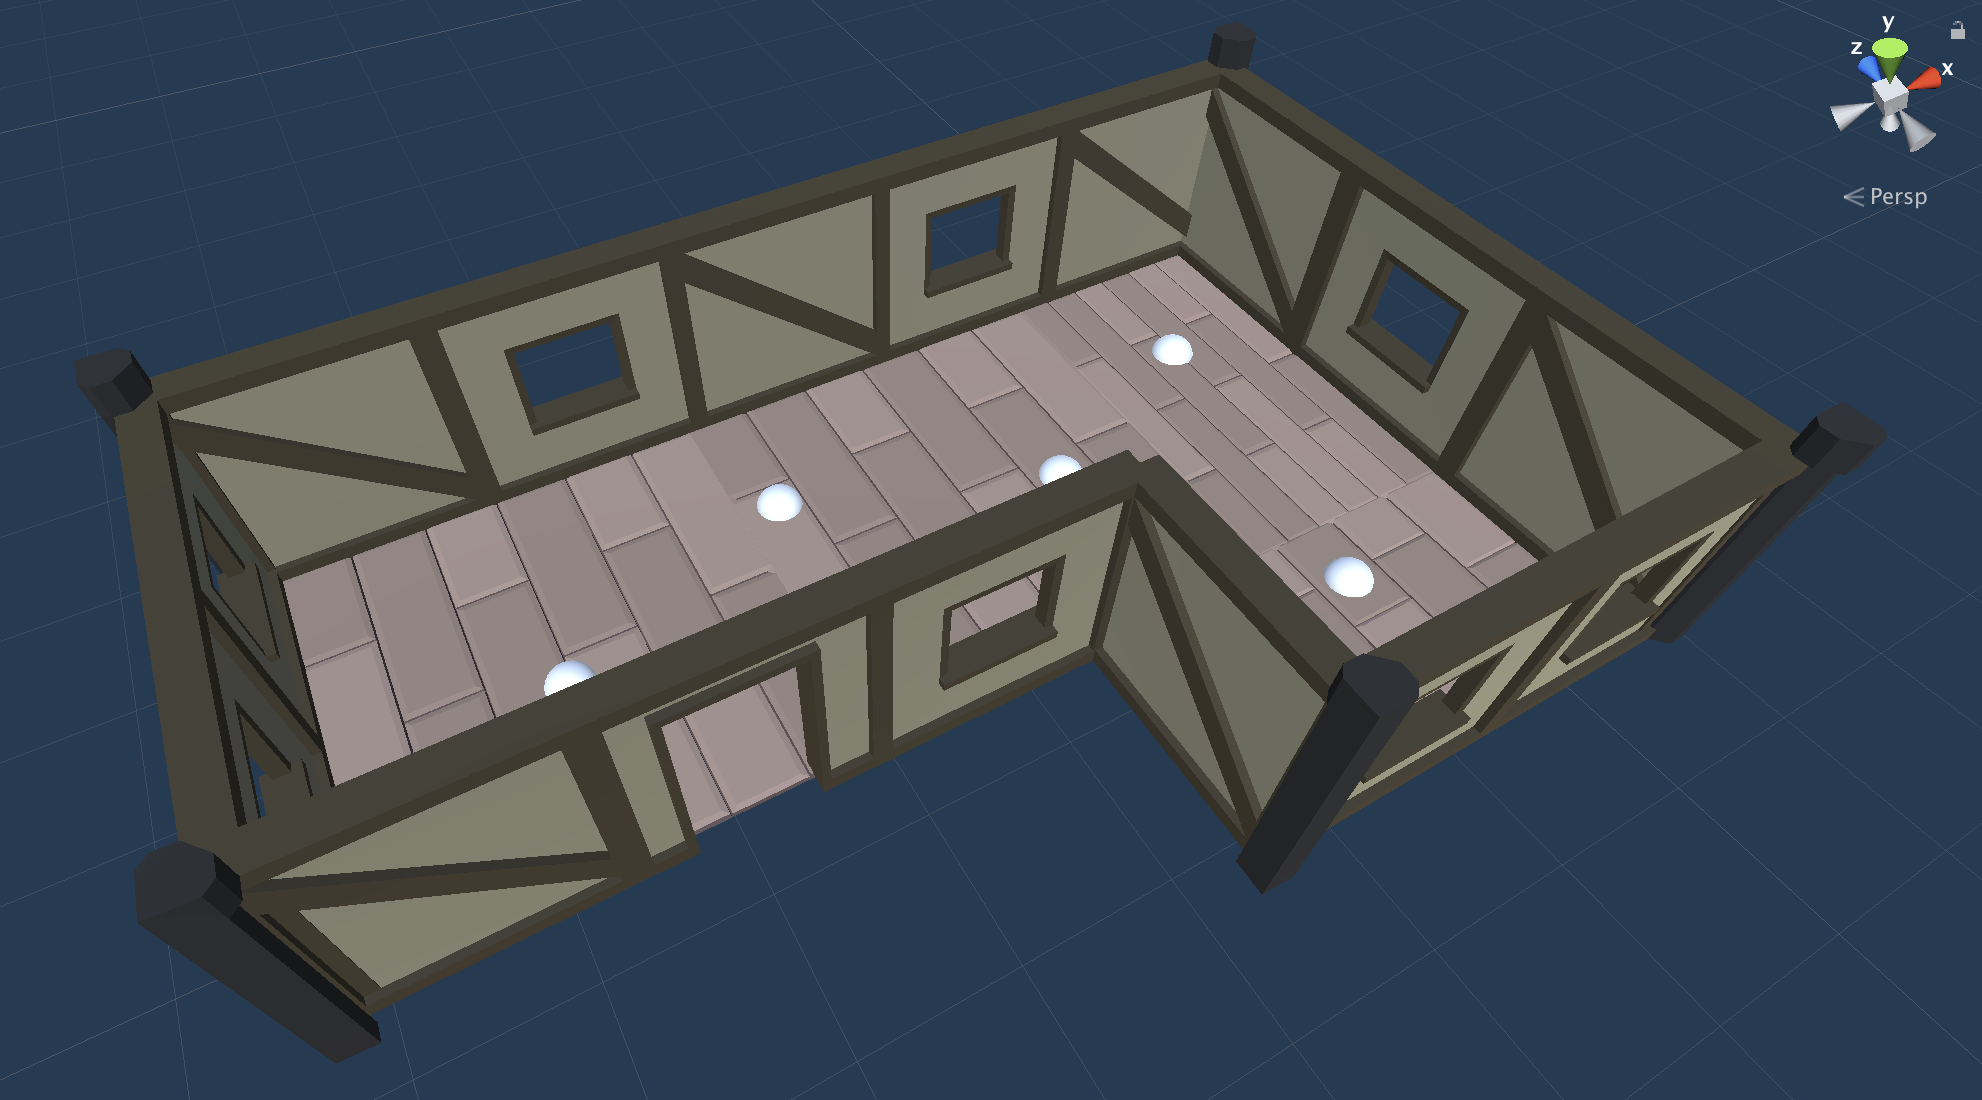
\includegraphics[scale=0.35]{images/village/village_navpoints_example.png}
\caption{Definition von \inlinecode{BuildingNavPoints} und \inlinecode{BuildingDistanceNavPoint}}
\label{fig:village_navpoints}
\end{figure}

\inlinecode{Building} enthält alle \inlinecode{BuildingNavPoint} des Gebäudes und verwaltet diese. Es werden Referenzen auf die bereits besetzten Slots in Gebäuden sowie den jeweiligen NPCs gehalten. Weiterhin ist für jeden Typ aus \inlinecode{LocationTypes} bekannt, wie viele offene Slots noch vorhanden sind.
Der \inlinecode{LocationHandler} bietet nun eine Menge von Funktionen. Diese stellen allesamt NPCs Orte zur Verfügung, unterscheiden sich jedoch leicht in ihrer Semantik:
\begin{itemize}
    \item \inlinecode{occupySlotInFoundBuilding} findet das erste Gebäude eines bestimmten Typs, das einen freien Slot hat und gibt die Position des ersten Slots in dem Gebäude zurück.
    \item \inlinecode{occupySlotInRandomBuilding} wird genutzt, um ein zufälliges Gebäude mit einem zufälligen Slot auszuwählen.
    \item \inlinecode{occupySlotInClosestBuilding} soll das nicht besetzte Gebäude finden, das sich von der Position des Agenten örtlich am wenigstens weit weg entfernt befindet.
    \item \inlinecode{occupySlotInNonEmptyBuilding} findet das erste Gebäude, das bereits mit mindestens einem Agenten besetzt ist. Falls kein Gebäude gefunden wird, wird eine zufällige Position zurückgegeben. Die Funktion wird unter anderem verwendet um zu simulieren, dass sich mehrere Agenten auf einem Marktplatz treffen, um miteinander zu kommunizieren. In diesem Fall wird stets ein Ort zurückgegeben, der bereits von einem \ac{npc} beansprucht wird, sodass diese sich \sogenannt{treffen} können und Gruppen entstehen.
\end{itemize}

Die Funktion \inlinecode{occupyFreeSlotInRandomBuilding} wird beispielhaft in Listing \ref{lst:village_location-handler_example} aufgeführt. Zunächst wird für alle Gebäude des Typs geprüft, ob sie über freie Plätze verfügen. Für diese Gebäude wird dessen Index in einer Liste gespeichert. Aus dieser Liste wird nun ein zufälliger Index \inlinecode{randomIndex} ausgewählt, der bestimmt, zu welchem Ort der Agent navigieren wird. In diesem Gebäude \inlinecode{chosenBuilding} wird ein Slot für den Agenten reserviert. Anschließend wird die Position des Slots, der einen \inlinecode{BuildingNavPoint} darstellt, anhand eines \inlinecode{Transform} in \inlinecode{\_calculatedPositions} hinterlegt. Später wird der Agent dieses Feld nutzen, um die Position abzufragen. Das ist nötig, weil die Funktion durch eine asynchrone Coroutine gestartet wird und diese deshalb keinen anderen Typen als \inlinecode{IEnumerator} zurückgeben kann (siehe Kapitel \ref{ml_unity}). Coroutinen werden bei der Gebäudesuche verwendet, um durch Threading eine höhere Leistung zu erreichen.

\begin{minipage}{\linewidth}
\begin{lstlisting}[linewidth=16.4cm, label=lst:village_location-handler_example, caption=Auswahl von zufälligen Gebäuden in der Klasse \inlinecode{LocationHandler} , xleftmargin=1cm]
public IEnumerator occupyFreeSlotInRandomBuilding(string locationType, int agentId, bool forceRandomSlot = false, bool getPositionOnly = false) {
    _calculatedPositions[agentId] = null;
    List<Building> locationTypeBuildings = _locations[locationType];
    List<int> freeBuildingIndices = new List<int>();
    int len = locationTypeBuildings.Count;
    for (int i = 0; i < len; i++) {
        if (!locationTypeBuildings[i].IsBuildingOccupied) freeBuildingIndices.Add(i);
    }
    if (freeBuildingIndices.Count == 0) {
        Debug.LogWarning("Attempted to occupy a free building for locationtype " + locationType + ", but there is none.");
        yield break;
    }
    int randomIndex = freeBuildingIndices[Mathf.RoundToInt(UnityEngine.Random.value * (freeBuildingIndices.Count - 1))];
    Building chosenBuilding = locationTypeBuildings[randomIndex];
    _agentsInBuildings[agentId] = chosenBuilding;

    Transform slotLocation = forceRandomSlot ? chosenBuilding.occupyRandomSlot(agentId) : chosenBuilding.occupySlot(agentId);
    if (slotLocation == null) {
        Debug.LogWarning("Failed to occupy free slot in random building for type " + locationType + ".");
        yield break;
    }
    _availableLocationTypeSlots[locationType]--;
    _calculatedPositions[agentId] = slotLocation;
    yield break;
}
\end{lstlisting}
\end{minipage}


Vor einer Zuweisung eines Agenten zu einem Slot kann die Funktion \inlinecode{hasFreeSpots} von außerhalb verwendet werden, um zu prüfen, ob Gebäude mit freien Plätzen existieren. Die Funktion prüft das Feld \inlinecode{private Dictionary<string, int> \_availableLocationTypeSlots}. Initial beschreibt das Feld die Gesamtanzahl der Slots, die für einen Gebäudetypen verfügbar sind. Jedes Mal wenn ein Agent einem Slot zugewiesen oder von ihm getrennt wird, wird die hinterlegte Anzahl für den Gebäudetypen angepasst.






\subsection{ResourceHandler}\label{resource_handler}
Es kommt ein Ressourcensystem zum Einsatz, bei dem die Klasse \inlinecode{ResourceHandler} als zentrale Verwaltungsstelle für alle Resourcen eines Dorfes agiert. Zu keiner Zeit verfügt ein Agent allein über eine Ressource, da der \inlinecode{ResourceHandler} alle im Dorf vorhandenen Ressourcen kennt und verwaltet. Aktionen können Ressourcen verbrauchen und Ressourcen produzieren. Daher nutzen besonders die Aktionen, die mit Berufen verbunden sind, das Ressourcensystem. Es sollen Abhängigkeiten von den NPCs untereinander geschaffen werden, da diese auf Ressourcen angewiesen sind, die von anderen NPCs produziert werden. Den Aktionen wird damit ein Sinn verliehen, der über die Bedürfnisbefriedigung und den visuellen Aspekt hinausgeht. Die Agenten sollen lernen, mit Ressourcen umzugehen.
Die Funktionen der Klasse sind in \ref{fig:architecture_diagram_resourcehandler} zu erkennen.

\begin{figure}[H]
\centering
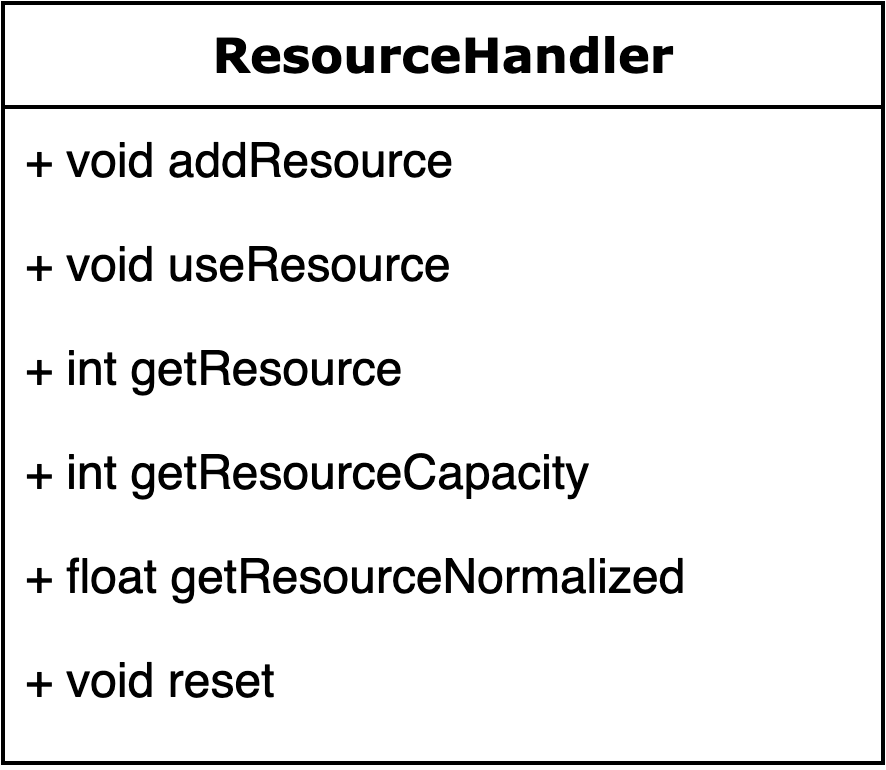
\includegraphics[scale=0.18]{images/village/architecture_diagram_resourcehandler.png}
\caption{Methoden der Klasse \inlinecode{ResourceHandler}}
\label{fig:architecture_diagram_resourcehandler}
\end{figure}

Eine Instanz des \inlinecode{ResourceHandler}s wird in der Klasse \inlinecode{Village} erzeugt und schließlich allen Agenten zugänglich gemacht. In der Funktion \inlinecode{reset} werden zunächst Obergrenzen für die Kapazitäten der einzelnen Ressourcen aufgrund der Anzahl der Agenten des Dorfes definiert. Je mehr Agenten vorhanden sind, desto höher ist die Kapazitätsgrenze, da sich die Menge der produzierten Ressourcen pro Aktion sowie die Menge der pro Agent verbrauchten Ressourcen nicht verändert. Weiterhin werden die Ressourcen zufällig initialisiert, werden aber durch Maximal- und Minimalwerte eingeschränkt. Die Funktion \inlinecode{reset} wird außerdem während des Trainings nach einer bestimmten Zeit aufgerufen, um die Ressourcen zurückzusetzen.
Die verschiedenen Typen von Ressourcen werden ebenfalls im \inlinecode{ResourceHandler} definiert. Über die Funktionen \inlinecode{addResource} und \inlinecode{useResource} können Agenten mit Ressourcen interagieren. Weiterhin besteht die Möglichkeit, in Abhängigkeit von der Kapazität einer Ressource durch die Funktion \inlinecode{getResourceNormalized} eine normalisierte Anzahl für eine Ressource zu erhalten. Der Wertebereich dieser Anzahl wird durch den Intervall $[0,1]$ definiert. Diese Normierung ist für die Observations wichtig, die idealerweise in dem genannten Intervall liegen sollten. Bei der Initialisierung der Simulation werden zufällige Werte für alle Ressourcen geliefert, die aber über einem Minimum und unter einem Maximum liegen.

\subsubsection{TimeController}
Der \inlinecode{TimeController} verwaltet das Voranschreiten der Zeit im Spiel. Der wird benötigt, um den Tagesablauf zu simulieren und die Bedürfnisse der Agenten aufgrund der vergangenen Zeit anzupassen. Abbildung \ref{fig:architecture_diagram_timecontroller} zeigt den Aufbau der Klasse.

\begin{figure}[H]
\centering
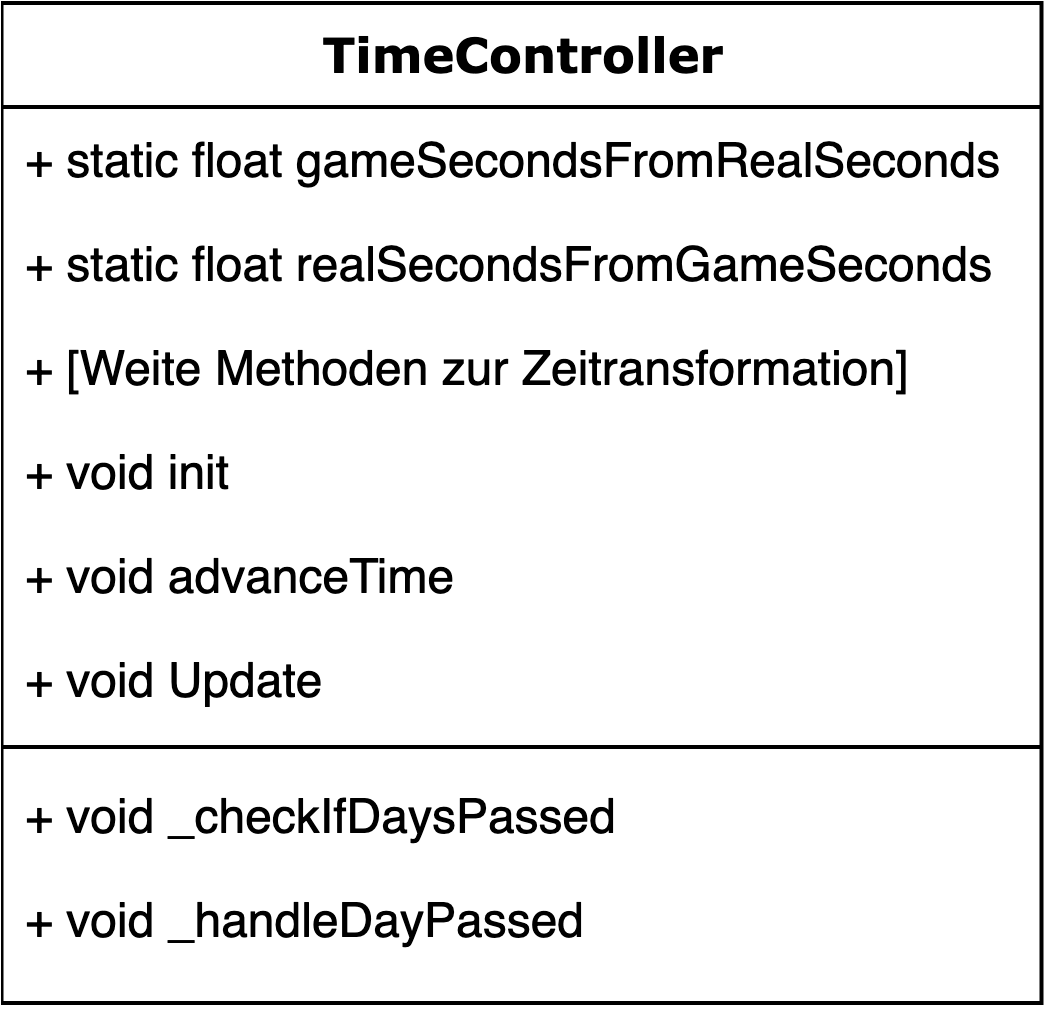
\includegraphics[scale=0.18]{images/village/architecture_diagram_timecontroller.png}
\caption{Methoden der Klasse \inlinecode{TimeController}}
\label{fig:architecture_diagram_timecontroller}
\end{figure}

Die Unityfunktion \inlinecode{Update} wird in Intervallen aufgerufen und ist dafür zuständig, alle Komponenten, die von der Zeit abhängig sind, mit der aktuellen Zeit zu versorgen. Konkret müssen der \inlinecode{LightHandler} und der \inlinecode{NpcState} jedes Agenten für jeden neuen Frame aktualisiert werden. Wie weit die Zeit voranschreitet, ist von der vergangen Zeit seit dem letzten Aufruf abhängig. Es wird in Sekunden gerechnet, da \inlinecode{Time.deltaTime} in Sekunden angegeben wird. Die Update-Funktion ruft für jeden neuen Frame die Funktion \inlinecode{advanceTime} auf:

\begin{minipage}{\linewidth}
\begin{lstlisting}[linewidth=16.4cm, label=lst:village_timecontroller_advancetime, caption=Funktion \inlinecode{advanceTime} im \inlinecode{TimeController}, xleftmargin=1cm]
public void advanceTime(float deltaTime) {
    _setCurrentTime(deltaTime);
    _village.updateTime(deltaTime, _currentTime, _daysPassed);
}
\end{lstlisting}
\end{minipage}

In der Funktion \inlinecode{\_setCurrentTime} findet anschließend die eigentliche Aktualisierung der Zeit statt:

\begin{minipage}{\linewidth}
\begin{lstlisting}[linewidth=16.4cm, label=lst:village_timecontroller_setcurrenttime, caption=Funktion \inlinecode{\_setCurrentTime} im \inlinecode{TimeController}, xleftmargin=1cm]
private void _setCurrentTime(float deltaTime) {
    _currentTime += deltaTime * ONE_SECOND_NORMALIZED * REAL_SECOND_INGAME_DURATION;
    _checkIfDaysPassed();
}
\end{lstlisting}
\end{minipage}

Wichtig ist dabei die Zeile 3. Die Konstante \inlinecode{ONE\_SECOND\_NORMALIZED} ist der auf einen ganzen Tag normierte Anteil einer Sekunde an diesem Tag:

$$ ONE\_SECOND\_NORMALIZED \;=\; \frac{1}{24 * 60 * 60} \approx 0.00012 $$

Der Wert von \inlinecode{\_currentTime} stellt die aktuelle Tageszeit dar, genormt auf einen Wert zwischen $0$ und $1$. Für jede im Spiel vergangene Sekunde wird \inlinecode{\_currentTime} also mit dem Wert $0.00012$ addiert. Im Spiel vergehen die Spiele jedoch schneller als in der Realität, weswegen \inlinecode{ONE\_SECOND\_NORMALIZED} mit \inlinecode{REAL\_SECOND\_INGAME\_DURATION} multipliziert wird.

Die Funktion \inlinecode{\_checkIfDaysPassed} prüft schließlich, ob ein Tag vergangen ist. Das ist der Fall, wenn $\_currentTime > 1f$.

\begin{minipage}{\linewidth}
\begin{lstlisting}[linewidth=16.4cm, label=lst:village_timecontroller_checkIfDaysPassed, caption=Funktion \inlinecode{\_checkIfDaysPassed} im \inlinecode{TimeController}, xleftmargin=1cm]
private void _checkIfDaysPassed() {
    _daysPassed = 0;
    while (_currentTime > 1f) {
        _days++;
        Monitor.Log("Days", _days.ToString());
        _currentTime -= 1f;
        _daysPassed += 1;
        _handleDayPassed();
    }
}
\end{lstlisting}
\end{minipage}

Die Funktion \inlinecode{advanceTime} ruft für jedes Update die Funktion \inlinecode{Village.updateTime} auf. Darin wird die neue Zeit an alle weiteren Komponenten weitergeleitet, die diese benötigen. Konkret sind das alle mit dem Dorf verbundenen Agenten mit ihren Bedürfnissen sowie der \inlinecode{LightHandler}:

\begin{minipage}{\linewidth}
\begin{lstlisting}[linewidth=16.4cm, label=lst:village_timecontroller_updatetime, caption=Funktion \inlinecode{updateTime} im \inlinecode{TimeController}, xleftmargin=1cm]
public void updateTime(float deltaTime, float currentTime, int daysPassed) {
    foreach (NpcAgent npc in _villageNpcs) {
        npc.updateNpc(deltaTime, currentTime, daysPassed);
    }
    _lightHandler.updateLights(currentTime);
}
\end{lstlisting}
\end{minipage}

Weiterhin bietet der \inlinecode{TimeController} durch die Funktionen \inlinecode{gameSecondsFromRealSeconds} und \inlinecode{realSecondsFromGameSeconds} sowie weiteren Methoden eine Schnittstelle für die Umrechnung zwischen Echtzeit und Spielzeit. In einer Konstante wird dafür die Dauer einer reellen Sekunde für spätere Berechnungen gespeichert. Zusätzlich wird ein normalisierter Wert für den Anteil einer Sekunde an einem Tag festgelegt:

\begin{minipage}{\linewidth}
\begin{lstlisting}[linewidth=16.4cm, label=lst:village_timecontroller_seconds_constants, caption=Berechnung der Dauer einer Sekunde in Simulationszeit, xleftmargin=1cm]
public const float REAL_SECOND_INGAME_DURATION = SECONDS_PER_DAY / DAY_CYCLE_REAL_SECONDS;
public const float ONE_SECOND_NORMALIZED = 1f / SECONDS_PER_DAY;
\end{lstlisting}
\end{minipage}

\inlinecode{SECONDS\_PER\_DAY} beträgt logischerweise $ 60 * 60 * 24 Sekunden $. Mithilfe dieser Werte kann die Realzeit nun in Simulationszeit umgerechnet werden:

\begin{minipage}{\linewidth}
\begin{lstlisting}[linewidth=16.4cm, label=lst:village_timecontroller_time_calculation, caption=Umrechnung von Simulationszeit und Realzeit, xleftmargin=1cm]
public static float realSecondsFromGameSeconds(float gameSeconds) {
    return gameSeconds / REAL_SECOND_INGAME_DURATION;
}

public static float gameSecondsFromRealSeconds(float realSeconds) {
    return ONE_SECOND_NORMALIZED * DAY_CYCLE_REAL_SECONDS * realSeconds;
}
\end{lstlisting}
\end{minipage}



\subsection{LightHandler}
Der \inlinecode{LightHandler} ist dafür zuständig, Tageszeiten zu simulieren, indem der Sonnenstand geregelt und Lichtquellen kontrolliert werden. In der Abbildung \ref{fig:architecture_diagram_lighthandler} wird der Aufbau der Klasse anhand ihrer Funktion verdeutlicht. 
Im \inlinecode{LightHandler} werden zusätzlich folgende Felder definiert:

\begin{itemize}
    \item \inlinecode{List<Light> \_agentLights}: Alle Lampen der Agenten. Jeder \ac{npc} verfügt über eine Lichtquelle, die sie an ihrem Körper tragen.
    \item \inlinecode{List<Light> \_villageLamps}: Alle Laternen, die im und um das Dorf herum positioniert wurden.
    \item \inlinecode{List<Light> \_bonfires}: Alle Lagerfeuer in der Simulation.
    \item \inlinecode{List<Transform> \_bonfireParticleTransforms}: Die Partikeleffekte der Lagerfeuer.
    \item \inlinecode{Light \_sun}: Eine Lichtquelle, die die Sonne simuliert.
\end{itemize}

\begin{figure}[H]
\centering
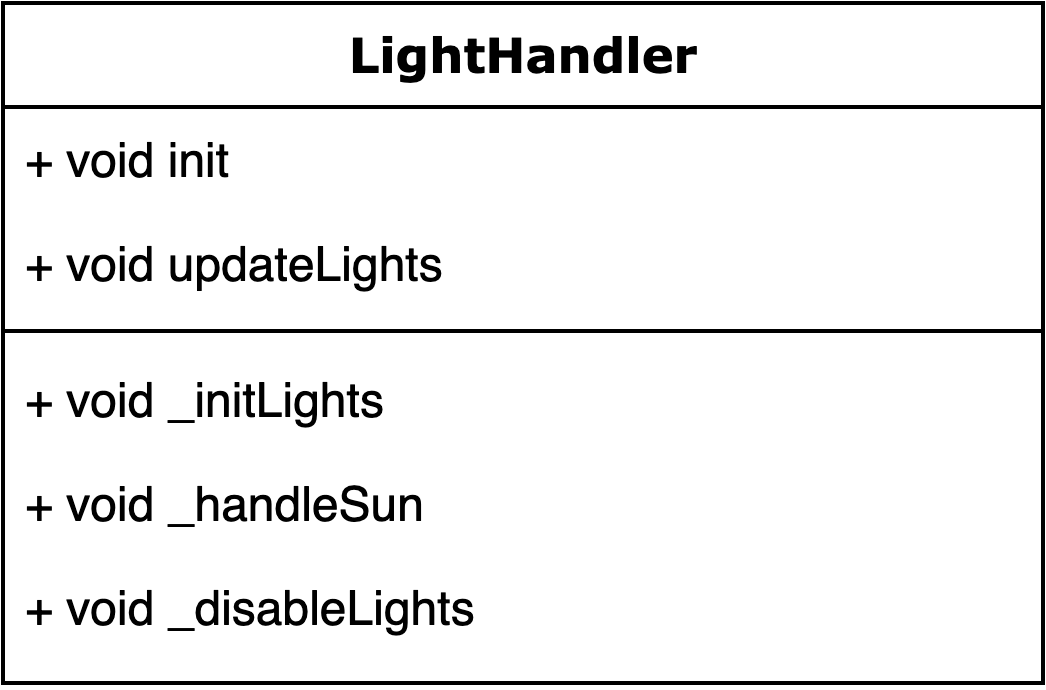
\includegraphics[scale=0.18]{images/village/architecture_diagram_lighthandler.png}
\caption{Methoden der Klasse \inlinecode{LightHandler}}
\label{fig:architecture_diagram_lighthandler}
\end{figure}

Die Funktion \inlinecode{\_initLights} sucht nach allen in der Szene enthaltenen Lichtquellen vom Typ \inlinecode{Light} und speichert diese. \inlinecode{Light} ist der Standardtyp für Lichtquellen in Unity. \inlinecode{Light} ist eine Komponente, die an ein \inlinecode{GameObject} angefügt wird.
Innerhalb der Funktion \inlinecode{updateLights} werden bestimmte Parameter der Lichtquellen in Abhängigkeit von der aktuellen Zeit verändert. Die Lichtquellen der Agenten sowie die Laternen im Dorf werden, zu einer bestimmten Uhrzeit an- und zu einer bestimmten Uhrzeit wieder ausgeschaltet. Nachts leuchten diese Lichtquellen also durchgehend. Weiterhin gibt es in der Stadt eine Menge von Lagerfeuern. Tagsüber glühen diese leicht, mit zunehmender Dunkelheit erhöht sich ihre Intensität. Die Partikeleffekte werden dann zusätzlich leicht nach oben verschoben, sodass sie weiter aus dem Boden herausragen und es so wirkt, als würde das Feuer stärker brennen. Jeder einzelne Partikel des Lagerfeuers stellt eine kleine Lichtquelle dar, um einen realistischen Feuereffekt zu simulieren.
Weiterhin wird in der Funktion \inlinecode{\_handleSun} sowohl die Intensität als auch die Position und Ausrichtung der Sonne in Abhängigkeit von der Zeit angepasst, wie in \ref{lst:lighthandler_sun} zu sehen.

\begin{minipage}{\linewidth}
\begin{lstlisting}[linewidth=16.4cm, label=lst:lighthandler_sun, caption=Anpassung der Sonne durch den \inlinecode{LightHandler}, xleftmargin=1cm]
private void _handleSun(float currentTime) {
    _sun.transform.localRotation = Quaternion.Euler((currentTime * 360f) - 90f, 170f, 0f);

    float multiplier = 1f;
    if (currentTime <= 0.28f) {
        multiplier = Mathf.Clamp01((currentTime - 0.25f) * (1f / 0.03f));
    }
    else if (currentTime >= 0.75f) {
        multiplier = Mathf.Clamp01(1f - ((currentTime - 0.78f) * (1f / 0.03f)));
    }
    _sun.intensity = multiplier * 1.5f;
}
\end{lstlisting}
\end{minipage}

Damit die Sonne sich wie eine Sonne verhält, muss die entsprechende Lichtquelle in den Lichteinstellungen der Unity-Szene als \Fachbegriff{Sun} markiert werden. Sie erhält dann automatisch das Aussehen einer Sonne und wird entsprechend positioniert. Unity übernimmt dann die eigentliche Beleuchtung und passt das \inlinecode{Light} so an, dass es eine überzeugende Sonne darstellt. Weiterhin verändert die Position der Sonne nun die Farbgebung der verwendeten Skybox - sobald die Sonne sich an den Rand des Horizonts bewegt, wird ein Sonnenuntergang bzw. Sonnenaufgang dargestellt. Wenn sie sich unter dem Horizont befindet, wird eine andere Textur für die Skybox verwendet, die in diesem Fall einen dunklen Sternenhimmel zeigt. Nun muss nur noch die Rotation der Sonne angepasst werden. Dadurch beschreibt die Position der Sonne im Verlauf des Tages eine Kreisbahn um das Dorf herum. Weiterhin wird die Intensität angepasst, sodass die Lichtverhältnisse mit der Tageszeit übereinstimmen. In den Abbildungen \ref{fig:village_village_night_1} und \ref{fig:village_village_night_2} ist beispielhaft zu erkennen, wie die Stadt nachts beleuchtet wird. Zum Vergleich wurden hier die selben Motive und Kameraeinstellungen verwendet, wie bereits in den Grafiken \ref{fig:village_village_day_1} und \ref{fig:village_village_day_2}.

\begin{figure}[H]
\centering
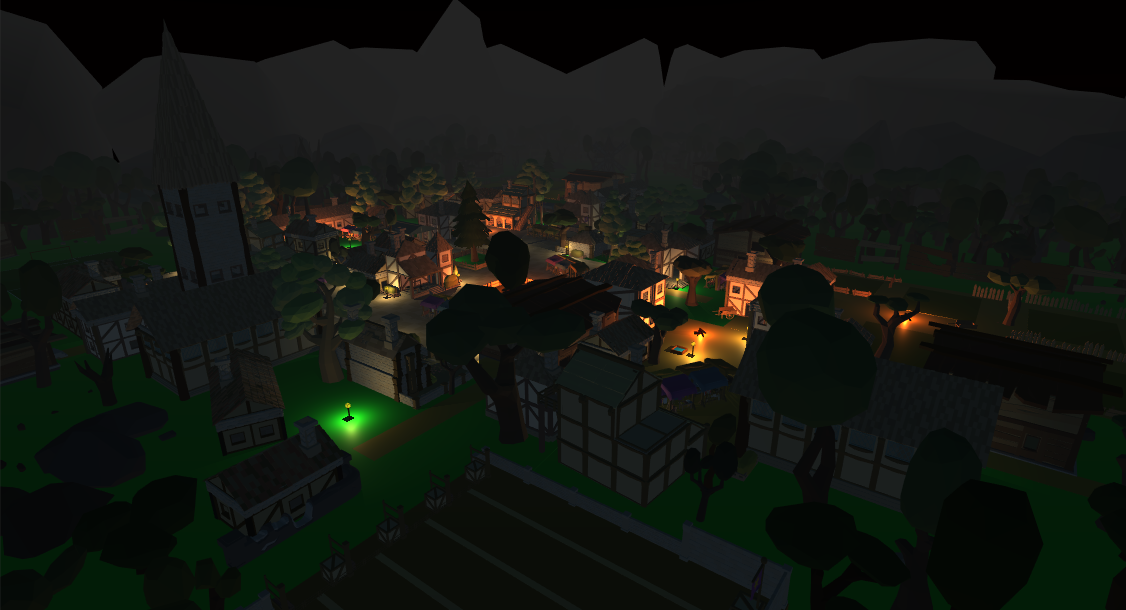
\includegraphics[scale=0.55]{images/village/village_village_night_1.PNG}
\caption{Modellierte Stadt, äußere Ansicht, nächtliche Beleuchtung}
\label{fig:village_village_night_1}
\end{figure}

\begin{figure}[H]
\centering
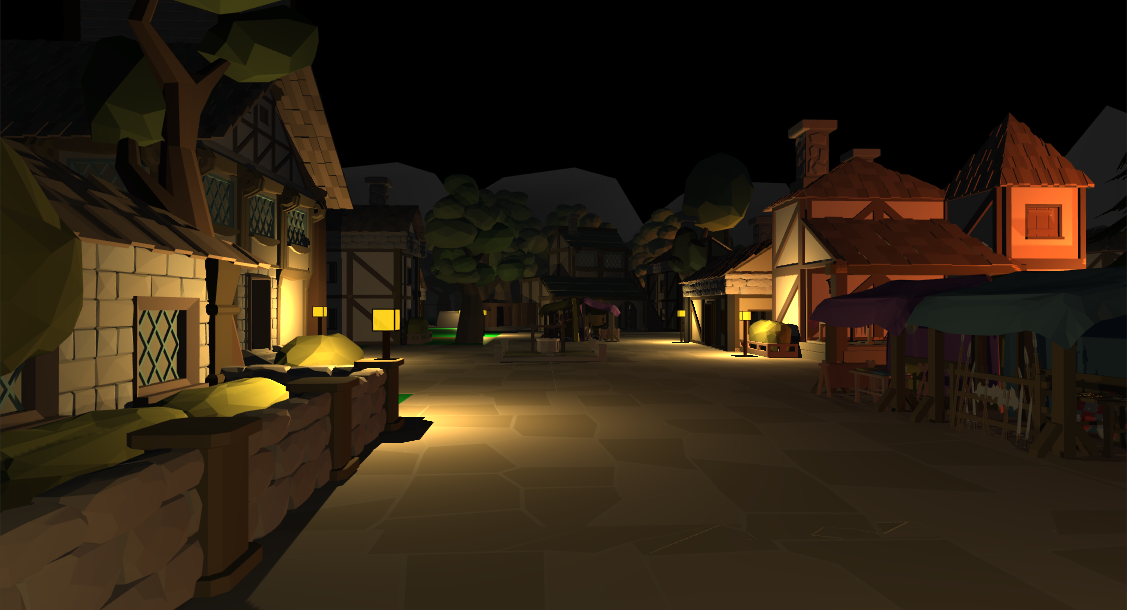
\includegraphics[scale=0.55]{images/village/village_village_night_2.png}
\caption{Modellierte Stadt, innere Ansicht, nächtliche Beleuchtung}
\label{fig:village_village_night_2}
\end{figure}


Für das Training des Agenten ist die Performance der Anwendung ausschlaggebend. Da die Entscheidungsfindung der Agenten in keiner Weise von der Beleuchtung der Szene abhängt, jedoch einen großen Teil der aufgewendeten Leistung in einer Simulation beansprucht, werden alle Lichtquellen während des Trainings automatisch deaktiviert. Dafür wird \inlinecode{GameAcademy.IS\_TRAINING} geprüft. In diesem Fall wird der \inlinecode{Lighthandler} nur initialisiert und dann deaktiviert, da keine Lichtquellen mehr zeitabhängig angepasst werden müssen.







\subsection{Implementierung des Agenten und dessen Subkomponenten}
Insgesamt wurden 16 Observations und 29 diskrete Aktionen verwendet, die dem Agenten zur Auswahl stehen. Es werden ausschließlich On Demand Decisions verwendet (siehe Kapitel \ref{ml_unity}). Der Agent wird während des Trainings nach einer festgelegten Anzahl von Entscheidungen zurückgesetzt. Das Training erfolgt mit dem \ac{ppo}-Algorithmus (siehe Abschnitt \ref{proximal_policy_optimization}) und verwendet ein neuronales Netz mit mehreren Schichten und mehreren hundert Neuronen. Es können beliebig viele Agenten verwendet werden. Zunächst werden die grundsätzlichen Funktionen der Klasse \inlinecode{NpcAgent} betrachtet, welche für die Realisierung der Agenten erstellt wurde.
Die Funktionen der Klasse werden in der Abbildung \ref{fig:architecture_diagram_agent} dargestellt.

\begin{figure}[H]
\centering
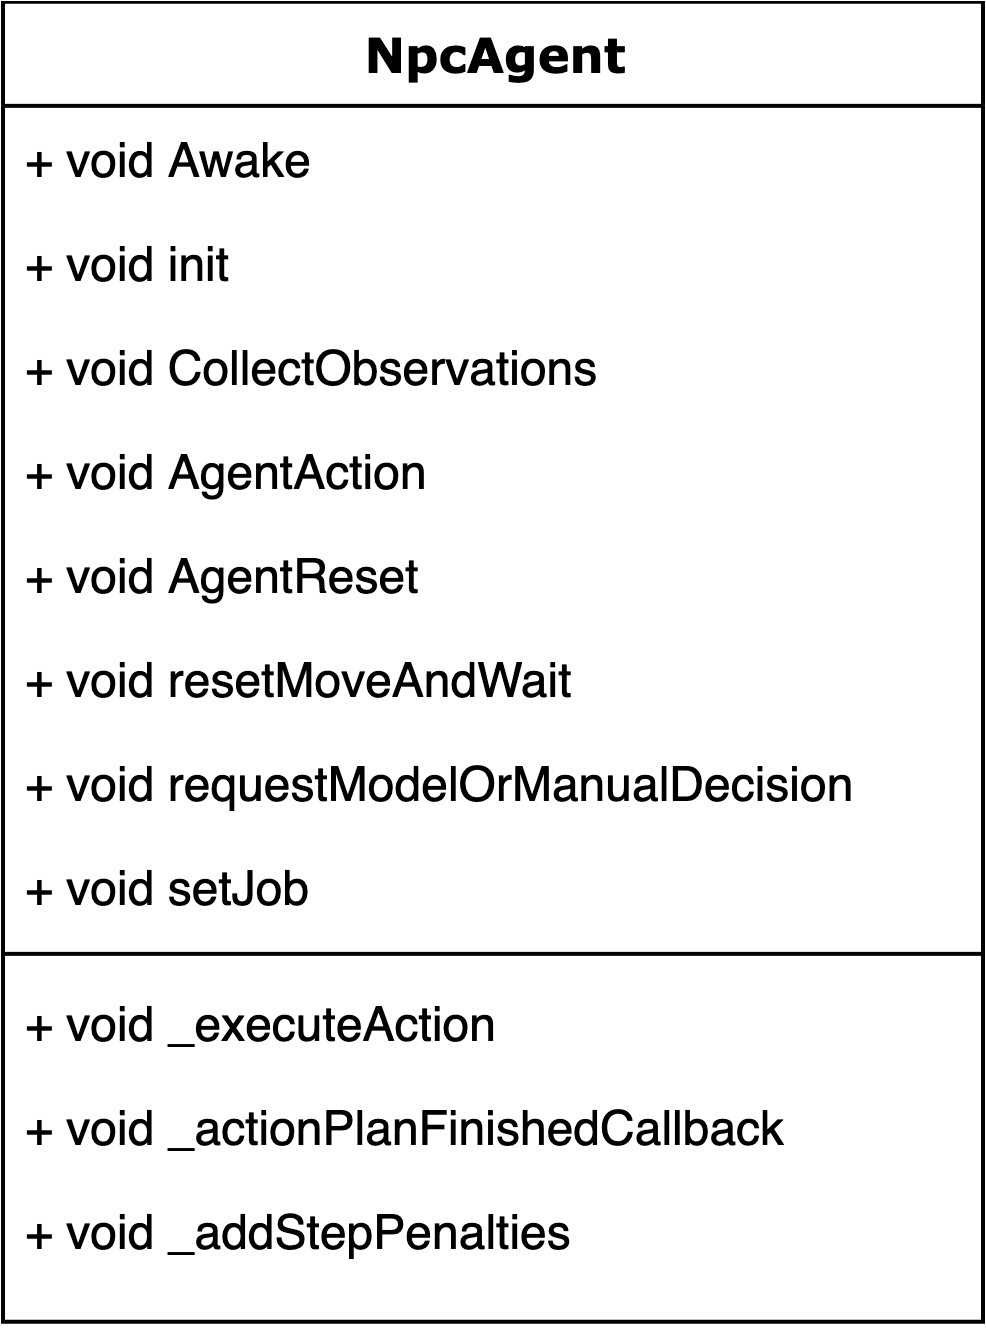
\includegraphics[scale=0.18]{images/village/architecture_diagram_agent.png}
\caption{Methoden der Klasse \inlinecode{NpcAgent}}
\label{fig:architecture_diagram_agent}
\end{figure}

Der \inlinecode{NpcAgent} verwendet sogenannte \Fachbegriff{ActionPlans} für die sequentielle Ausführung von Aktionen. Diese werden im späteren Abschnitt \ref{action_plans} behandelt.

Die Funktionen \inlinecode{CollectObservations}, \inlinecode{AgentAction}, \inlinecode{AgentReset} und \inlinecode{Awake} sind bereits bekannt (siehe Kapitel \ref{ml_unity}).
Die Funktionen \inlinecode{Awake} \inlinecode{setJob} und \inlinecode{init} werden benötigt, um den Agenten zu intitialisieren. Weiterhin werden \inlinecode{resetMoveAndWait} und \inlinecode{AgentReset} verwendet, um den Agenten beispielsweise nach dem Abschließen einer Episode zurückzusetzen. In der Funktion \inlinecode{\_actionPlanFinishedCallback} wird nach dem Ausführen einer Aktion geprüft, ob eine Episode abgeschlossen ist oder eine neue Entscheidung mit \inlinecode{requestModelOrManualDecision} angefragt werden soll. In der Funktion \inlinecode{\_addStepPenalties} werden darüber hinaus Bestrafungen ausgeschüttet. Konkret wird für jedes Bedürfnis des Agenten, das unter einer bestimmten Grenze liegt, eine Bestrafung zugewiesen.

Der Beobachtungsraum des Agenten wird durch die in der Funktion \inlinecode{CollectObservations} getätigten Observations beschrieben, wie in Listing \ref{lst:village_agent_observations} zu sehen:

\begin{minipage}{\linewidth}
\begin{lstlisting}[linewidth=16.4cm, label=lst:village_agent_observations, caption=Beobachtungen des Agenten, xleftmargin=1cm]
public override void CollectObservations() {
    AddVectorObs(_npcState.NeedHunger);
    AddVectorObs(_npcState.NeedThirst);
    AddVectorObs(_npcState.NeedEducation);
    AddVectorObs(_npcState.NeedCommunication);
    AddVectorObs(_npcState.NeedFaith);
    AddVectorObs(_npcState.Recreation);
    AddVectorObs(_npcState.Exhaustion);
    AddVectorObs(_npcState.AttFittness);
    AddVectorObs(_npcState.AttIntelligence);
    AddVectorObs(_npcState.AttCompanionship);
    AddVectorObs(_npcState.AttCommodities);
    AddVectorObs(_npcState.AttFerocity);
    AddVectorObs(_npcState.Sleep);
    AddVectorObs(_npcState.Work);
    AddVectorObs(_npcState.getMoneyNormalized());
    AddVectorObs(_currentTime);

    SetActionMask(_actionMaskingHandler.getIntActionMask(this));
}
\end{lstlisting}
\end{minipage}

Als Input für das neuronale Netz werden also sämtliche Bedürfnisse sowie die Attribute, die Menge des Geldes des Agenten und die aktuelle Zeit verwendet. Insgesamt kommen so 16 Observations zustande.
Der Handlungsraum besteht aus 29 möglichen Aktionen für die Befriedigung von Bedürfnissen. Die Funktion \inlinecode{AgentAction} ist in Listing \ref{lst:agent_agentaction} zu erkennen:

\begin{minipage}{\linewidth}
\begin{lstlisting}[linewidth=16.4cm, label=lst:agent_agentaction, caption=Funktion \inlinecode{AgentAction} des Agenten, xleftmargin=1cm]
public override void AgentAction(float[] vectorAction, string textAction) {
    _executeAction(NpcActions.actionNameFromId(Mathf.RoundToInt(vectorAction[0])));
}

private void _executeAction(string actionId) {
    [...] // Logging etc.
    _action = actionId;
    _academy.IncrementNumAgentActions();
    _numActions++;
    _actionHandler.runActionPlan(actionId);
}
\end{lstlisting}
\end{minipage}

Zunächst wird aus dem Float-Wert, der von ML-Agents geliefert wird, ein Integer gemacht. Das ist sinnvoll, weil hier diskrete Entscheidungen verwendet werden, die durch einen Integer-Wert referenziert werden. In der Funktion \inlinecode{\_executeAction} werden schließlich nach einigen Logging-Anweisungen Zähler inkrementiert und durch die Anweisung \inlinecode{\_actionHandler.runActionPlan} der \inlinecode{ActionHandler} aufgerufen, der dem Identifier der Aktion einen ausführbaren ActionPlan zuweist. Im nächsten Abschnitt wird dieses Vorgehen erläutert. Es wird darauf eingegangen, wie die Aktionen des Agenten beschrieben und ausgeführt werden können.


\subsubsection{ActionPlans}\label{action_plans}
Für die Ausführung von Aktionen wurde eine eigene Kontroll- und Datenstruktur entwickelt, die eine Reihe von untergeordneten Aktionen enthält. Die Struktur ist allgemein für sequentielle Ausführungen von Aufgaben nutzbar, deren zeitliche Dauer zum Zeitpunkt der Ausführung unbekannt sein kann. In dieser Arbeit wurden diese \Fachbegriff{ActionPlans} genannten Konstrukte für die Ausführung der Aktionen des Agenten angefertigt. Im Folgenden werden sie näher erläutert.
ActionPlans erben von der Basisklasse \inlinecode{BaseActionPlan}. Die Abbildung \ref{fig:architecture_diagram_baseactionplan} zeigt die Funktionen der Klasse:

\begin{figure}[H]
\centering
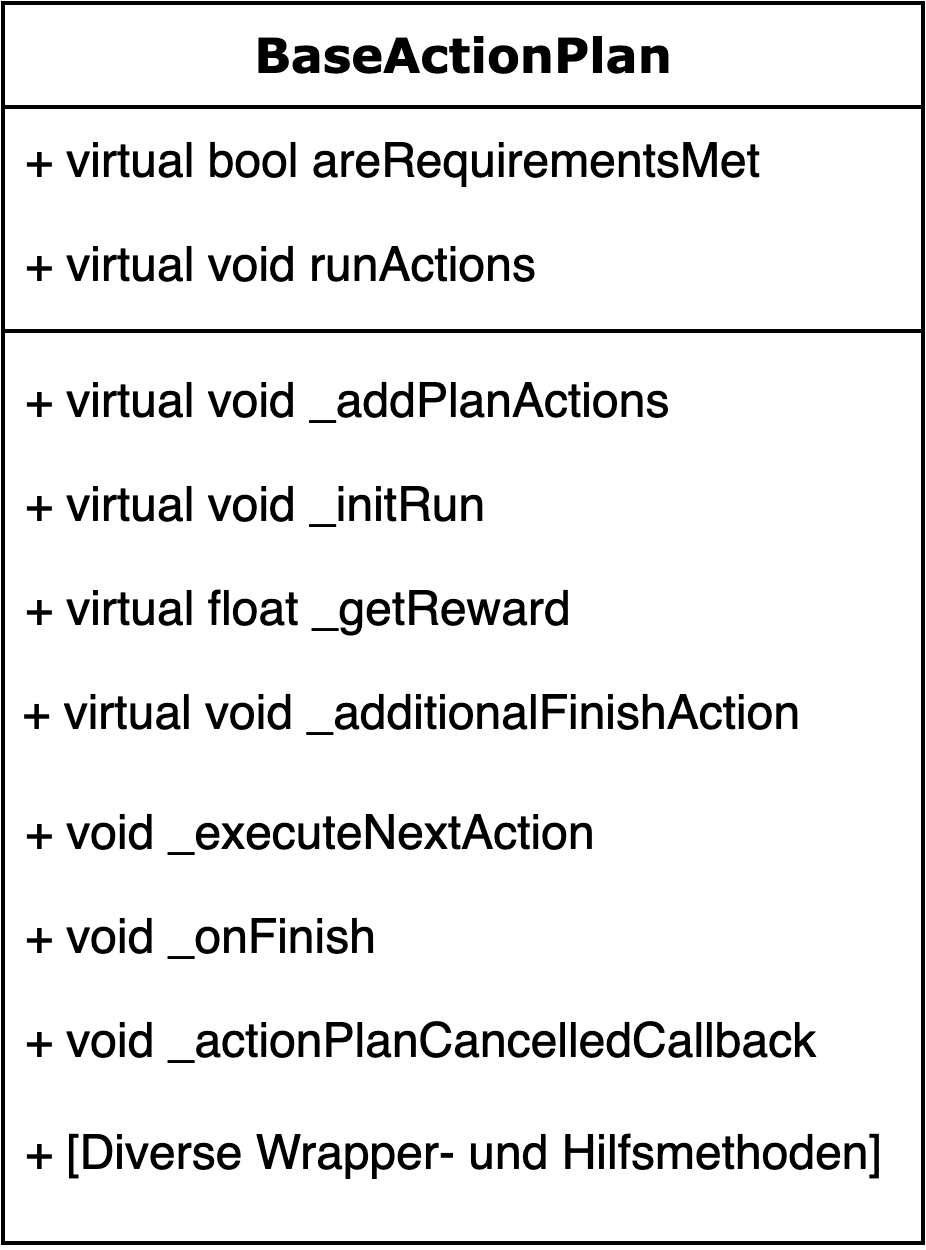
\includegraphics[scale=0.18]{images/village/architecture_diagram_baseactionplan.png}
\caption{Methoden der Klasse \inlinecode{BaseActionPlan}}
\label{fig:architecture_diagram_baseactionplan}
\end{figure}

In der Klasse \inlinecode{NpcActions} werden String-Identifier für alle Aktionen definiert, zum Beispiel \inlinecode{NpcActions.HUNGER\_BREAD}. \inlinecode{NpcActions} liefert weiterhin ein Mapping dieser Identifier zu den numerischen Identifiern von Aktionen, die ML-Agents beim Aufruf der Funktion \inlinecode{AgentAction} liefert. Anhand dieser Identifier wird jeder Aktion aus dem Aktionsraum des neuronale Netzes genau ein übergeordneter ActionPlan zugewiesen. 
Die Menge aller Sub-Aktionen eines ActionPlans beschreibt genau eine übergeordnete Aktion. Von der Basisklasse \inlinecode{BaseActionPlan} müssen bestimmte Funktionen überschrieben werden. Innerhalb der Funktion \inlinecode{\_addPlanActions} werden eine Reihe von Aktionen definiert, die sequentiell ausgeführt werden, wie beispielsweise das Navigieren des Agenten zu einer Zielposition. Zusätzlich zur Ausführung von Aktionen werden hier Effekte und Voraussetzungen für Aktionen verwaltet. Die Ausführung der einzelnen Teilaktionen erfolgt in der Funktion \inlinecode{nextActionExecutedCallback}. Nach der Ausführung jeder Einzelaktion wird ein Callback aufgerufen, wie in Listing \ref{lst:village_actionplan_single_action_callback} zu erkennen. Es handelt sich um eine einfache Funktion ohne Parameter, die jeder Einzelaktion im Konstruktor mitgegeben wird.

\begin{minipage}{\linewidth}
\begin{lstlisting}[linewidth=16.4cm, label=lst:village_actionplan_single_action_callback, caption=ActionPlan-Callback, xleftmargin=1cm]
private void nextActionExecutedCallback()
{
    _currentAction += 1;

    if (_currentAction >= _actions.Count) {
        _onFinish();
        _allActionsExecutedCallback();
    } else {
        _executeNextAction();
    }
}
\end{lstlisting}
\end{minipage}

Wenn weitere Aktionen vorhanden sind, wird die nächste Aktion aus der Liste ausgeführt. Auf die Terminierung der letzten Aktion folgt der Aufruf eines weiteren, übergeordneten Callbacks \inlinecode{\_allActionsExecutedCallback}. Auch hier handelt es sich um eine einfache parameterlose Funktion. Der Callback ruft im \inlinecode{NpcAgent} die Funktion \inlinecode{\_actionPlanFinishedCallback} auf und führt zu einer Anfrage an das ML-Agents Toolkit für eine neue Entscheidung. Nach der Ausführung der Aktionen wird weiterhin eine Belohnung oder eine Bestrafung für den Agenten ausgeschüttet, indem \inlinecode{\_onFinish} aufgerufen wird. Zusätzlich können abschließend beispielsweise Ressourcen hinzugefügt werden, die die Aktion produziert hat.

Zum Start des ActionPlans wird die in Listing \ref{lst:village_actionplan_runactions} dargestellte Funktion \inlinecode{runActions} verwendet:

\begin{minipage}{\linewidth}
\begin{lstlisting}[linewidth=16.4cm, label=lst:village_actionplan_runactions, caption=Starten eines ActionPlans, xleftmargin=1cm]
public void runActions() {
    _npc.VillageInfo.changeAmountForAction(true, _actionType);
    _currentAction = 0;
    _initRun();

    if (_actions == null || _actions.Count == 0) {
        _onFinish();
        _allActionsExecutedCallback();
    } else {
        _executeNextAction();
    }
}
\end{lstlisting}
\end{minipage}

Im Konstruktor von \inlinecode{BaseActionPlan} wird die abstrakte Funktion \inlinecode{\_addPlanActions} definiert, welche von Unterklassen überschrieben werden muss. Darin müssen die Aktionen des ActionPlans hinzugefügt werden, indem sie durch \inlinecode{\_actions.Add(newAction)} in eine \inlinecode{List<BaseAction>} geschrieben werden. In \inlinecode{runActions} wird zunächst die erste dieser Aktionen mit dem Index $\_currentAction = 0$ ausgeführt. Nach jeder ausgeführten Aktion wird der Index erhöht und die nächste Funktion ausgeführt.

Ein Beispiel für eine Implementierung eines vollständigen ActionPlans ist in \ref{lst:village_butcher-actionplan} zu finden. Der ActionPlan \inlinecode{ReligionChurchActionPlan} beschreibt den Vorgang eines Agenten, die Kirche zu besuchen, um sein Bedürfnis nach \Fachbegriff{Glauben} aufzufüllen.

\begin{minipage}{\linewidth}
\begin{lstlisting}[linewidth=16.4cm, label=lst:village_butcher-actionplan, caption=Beispielhafter ActionPlan \inlinecode{ReligionChurchActionPlan}, xleftmargin=1cm, basicstyle=\footnotesize]
public class ReligionChurchActionPlan : BaseActionPlan
{
    public ReligionChurchActionPlan(Action allActionsExecutedCallback,
                                   NpcAgent npc)
        : base(NpcActions.RELIGION_CHURCH, allActionsExecutedCallback, npc) { }

    public override bool areRequirementsMet() {
        if (!_hasFreeSpot(LocationTypes.CHURCH)) return false;
        return true;
    }

    protected override float _getReward() {
        return _getNeedReward(NpcState.NEED_FAITH, NEED_REWARD_MULTIPLIER);
    }

    protected override void _addPlanActions() {
        _addMoveAction(LocationTypes.CHURCH);
        _addWaitAction(DEFAULT_ACTION_SECONDS);
        _addVacateAction(LocationTypes.CHURCH);
    }

    protected override void _additionalFinishAction() {
        _npcState.satisfyNeedByType(NpcState.NEED_FAITH, DEFAULT_NEED_GAIN);
    }
}
\end{lstlisting}
\end{minipage}

Bevor die Entscheidung getroffen wird, welcher ActionPlan ausgeführt werden soll, wird die Funktion \inlinecode{areRequirementsMet} jedes ActionPlans aufgerufen. Diese prüft einige Bedingungen, die erfüllt sein müssen, damit der ActionPlan ausgeführt werden darf. Die Voraussetzung für die Ausführung in dem obigen Beispiel stellt die Bedingung auf, dass mindestens ein freier Slot in einem Gebäude des Typs \inlinecode{CHURCH} vorhanden sein muss.
Die einzelnen Teilaktionen des ActionPlans werden in \inlinecode{\_addPlanActions} definiert. Zunächst wird eine \inlinecode{MoveAction} definiert, die den Agenten zur Kirche bewegt. Diese Aktion beinhaltet die Reservierung eines Slots für den Agenten. Weiterhin wird eine \inlinecode{WaitAction} definiert, welche typischerweise genutzt wird, um die Ausführung einer beliebigen Tätigkeit zu simulieren. Effektiv bleibt der Agent an einem Ort stehen und wartet, bis eine gewisse Zeit abgelaufen ist. Anschließend wird eine \inlinecode{VacateAction} ausgeführt, welche dafür sorgt, dass zum Ende des Ausführungsprozesses des ActionPlans der reservierte Slot für den Agenten wieder freigegeben wird.
Nach der Ausführung der Aktionen wird schließlich durch die Funktion \inlinecode{\_getReward} die Belohnung definiert. Diese hängt von dem initialen Bedürfnis nach Glauben ab, das zu Beginn der Ausführung des ActionPlans festgestellt wurde. Der Vorgang wird im \inlinecode{BaseActionPlan}, unter anderem in der Funktion \inlinecode{\_initRun}, beschrieben. Als letztes wird das Bedürfnis des Agenten nach Glauben aufgefüllt.

Alle ActionPlans eines Agenten werden im \inlinecode{ActionHandler} erzeugt. Mithilfe des in \inlinecode{NpcActions} definierten Mappings werden die ActionPlans in einem \inlinecode{Dictionary<String,BaseActionPlan>} hinterlegt. Sobald eine neue Aktion des Agenten mit \inlinecode{AgentAction} gestartet wird, wählt der \inlinecode{ActionHandler} den zum Identifier der Aktion passenden ActionPlan aus.

In der Abbildung \ref{fig:architecture_diagram_actionhandler} ist der Aufbau der Klasse \inlinecode{ActionHandler} zu erkennen:

\begin{figure}[H]
\centering
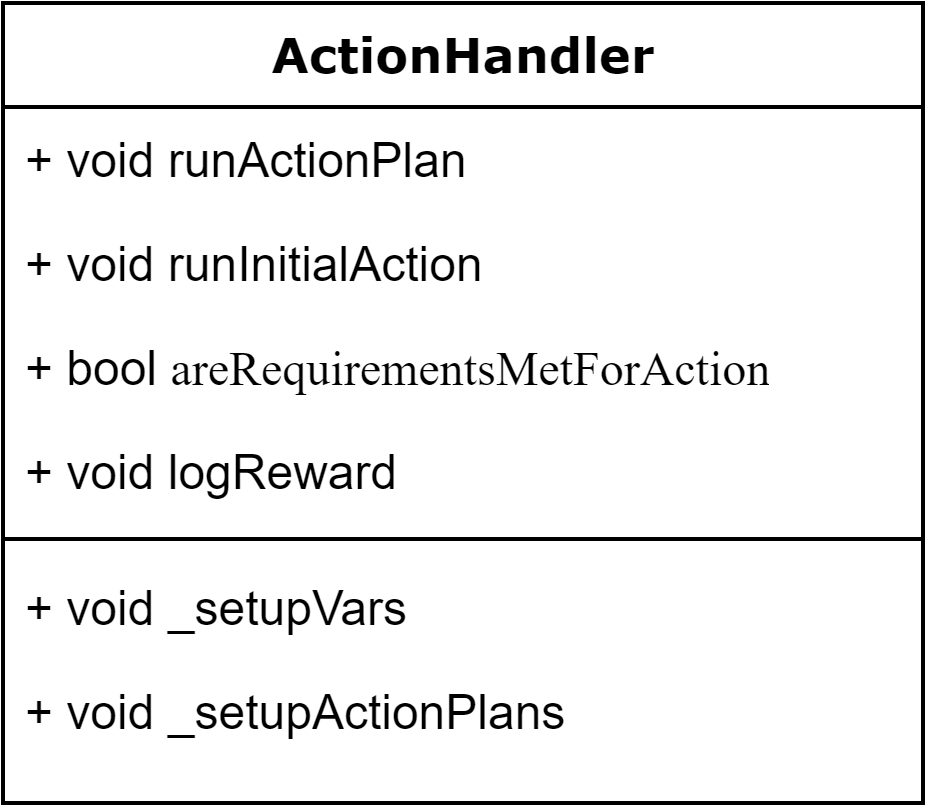
\includegraphics[scale=0.18]{images/village/architecture_diagram_actionhandler.png}
\caption{Methoden der Klasse \inlinecode{ActionHandler}}
\label{fig:architecture_diagram_actionhandler}
\end{figure}

Die Funktion \inlinecode{runInitialAction} wird verwendet, um nach der Initialisierung des Dorfes für jeden Agenten eine \inlinecode{WaitAction} mit zufälliger Dauer durchzuführen, sodass nicht alle Agenten zur selben Zeit anfangen, Aktionen auszuführen. Damit wird vermieden, dass Engpässe bezüglich der Kapazität bestimmter Gebäude entstehen.
Die Funktion \inlinecode{areRequirementsMetForAction} dient lediglich als Wrapper für die \inlinecode{areRequirementsMet}-Funktionen der einzelnen ActionPlans und wird vom \inlinecode{ActionMaskingHandler} aufgerufen.


\paragraph{Belohnungen}
Die Belohnungen der Aktionen des Agenten werden ebenfalls in den ActionPlans definiert. Dafür wurde eine Reihe von Hilfsfunktionen erstellt, zum Beispiel \inlinecode{\_getNeedReward} oder \inlinecode{\_getRecreationReward}. Die Zusammensetzung der Belohnungen kann in den jeweiligen ActionPlans im Programmcode betrachtet werden.


\paragraph{Teilaktionen des ActionPlans}
Zusätzlich zu den genannten Methoden werden diverse weitere Wrapper- und Hilfsmethoden implementiert, wie beispielsweise die Funktion \inlinecode{\_moveAndWaitRealSeconds}, die automatisch die Teilaktionen \inlinecode{MoveAction}, \inlinecode{VacateAction} und \inlinecode{WaitAction} hinzufügt, um zu einem Ort zu navigieren und dort zu verweilen. Diese Teilaktionen des ActionPlans erben von der Klasse \inlinecode{BaseAction}. Die Implementierung dieser Basisklasse ist im folgenden Listing zu erkennen:

\begin{minipage}{\linewidth}
\begin{lstlisting}[linewidth=16.4cm, label=lst:implementation_baseaction, caption=Implementierung von \inlinecode{BaseAction}, xleftmargin=1cm, basicstyle=\footnotesize]
public class BaseAction {
    protected string _actionType;
    protected NpcAgent _npc;
    protected TimeController _timeController;

    public BaseAction(string actionType, NpcAgent npc) {
        _actionType = actionType;
        _npc = npc;
        _timeController = GameObject.FindObjectOfType<TimeController>();
    }

    public virtual IEnumerator execute(Action callback,
                                       Action cancelCallback) {
        throw new System.NotImplementedException("Function execute not implemented for " + this.GetType());
    }
}
\end{lstlisting}
\end{minipage}

Klassen, die von \inlinecode{BaseAction} erben, müssen nur die \inlinecode{execute}-Funktion überschreiben und eine Callbackfunktion aufrufen, sobald die Teilaktion abgeschlossen wurde.

Um den Agenten zu einem Zielort zu bewegen wird die \inlinecode{MoveAction} verwendet. Diese interagiert zunächst mit dem \inlinecode{LocationHandler}, um einen Zielort zu erlangen und schließlich mit dem \inlinecode{MoveHandler}, um den Agenten zum Ziel zu navigieren. In der Abbildung \ref{fig:architecture_diagram_movehandler} wird der Aufbau der Klasse \inlinecode{MoveHandler} verdeutlicht:

\begin{figure}[H]
\centering
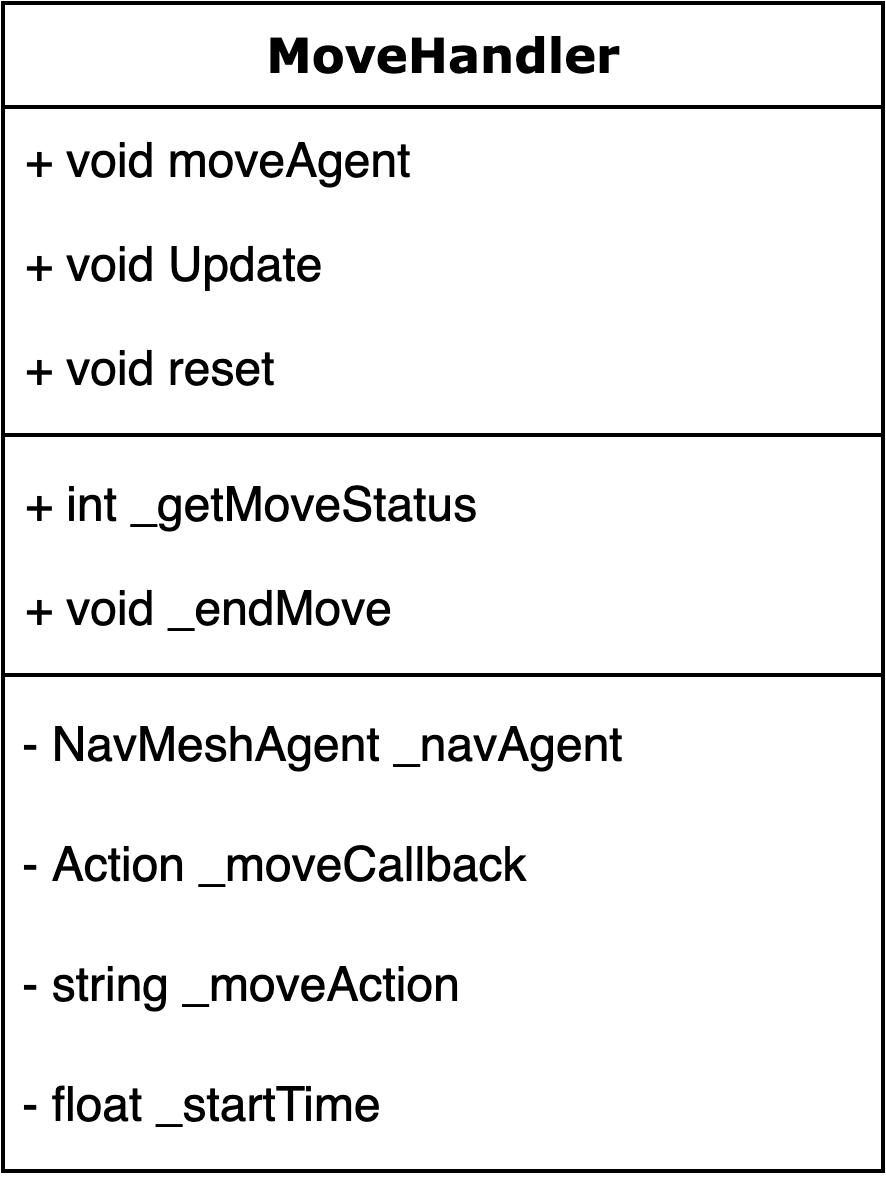
\includegraphics[scale=0.18]{images/village/architecture_diagram_movehandler.png}
\caption{Methoden der Klasse \inlinecode{MoveHandler}}
\label{fig:architecture_diagram_movehandler}
\end{figure}

Die Funktion \inlinecode{moveAgent} startet die Navigation zum Ziel. Das Feld \inlinecode{\_navAgent} referenziert den \inlinecode{NavMeshAgent}, der verwendet wird, um auf dem NavMesh zu navigieren (siehe Abschnitt \ref{agent_navigation}). Durch die Anweisung \inlinecode{\_navAgent.SetDestination(destination)} wird die Navigation des Agenten zu seinem Zielort gestartet. Zu Logging-Zwecken wird außerdem die Startzeit der Aktion im Feld \inlinecode{\_startTime} gespeichert. Die \inlinecode{Update}-Funktion prüft anschließend mit jedem neuen Frame den Status des Agenten mithilfe der Funktion \inlinecode{\_getMoveStatus}. Sobald diese Funktion den Status \inlinecode{MOVE\_STATUS\_STOPPED} zurückgibt, hat der Agent sein Ziel erreicht und ein Callback wird aufgerufen, um zurück zur \inlinecode{MoveAction} zu springen, welche wiederum einen weiteren Callback zum jeweiligen ActionPlan ausführt.

\begin{figure}[H]
\centering
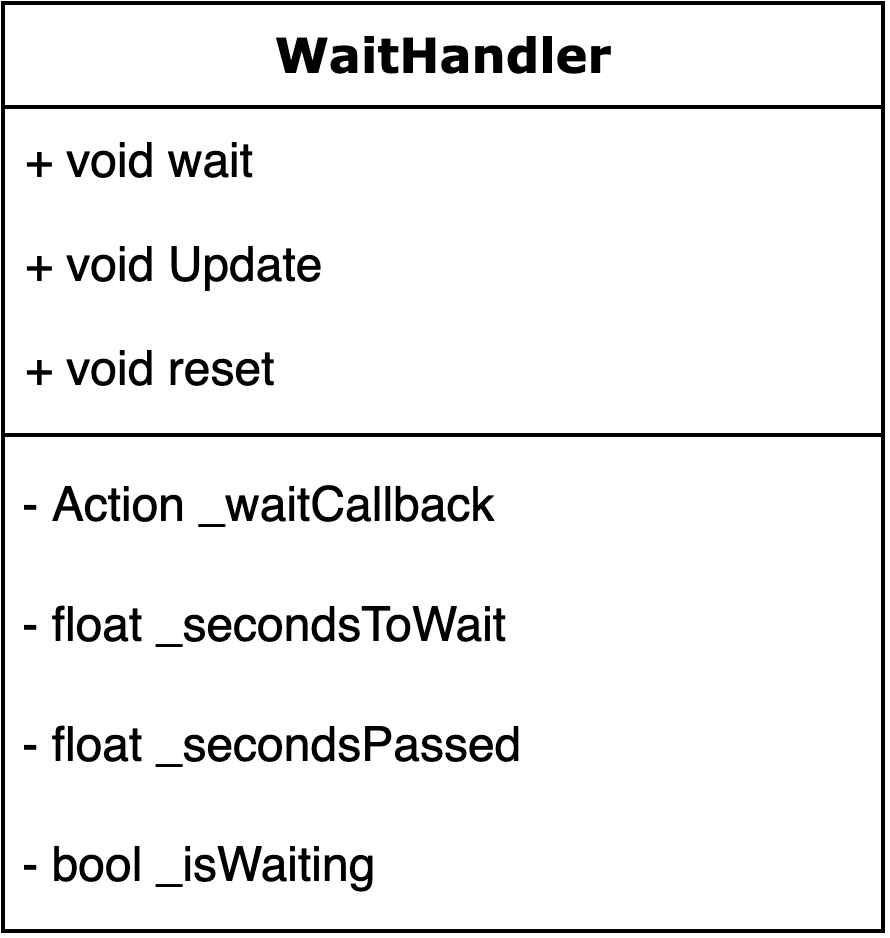
\includegraphics[scale=0.18]{images/village/architecture_diagram_waithandler.png}
\caption{Methoden der Klasse \inlinecode{WaitHandler}}
\label{fig:architecture_diagram_waithandler}
\end{figure}

Eine weitere essentielle Teilaktion ist die \inlinecode{WaitAction}. Diese funktioniert grundsätzlich wie die \inlinecode{MoveAction}, gibt dem zugrunde liegenden \inlinecode{WaitHandler} jedoch kein örtliches Ziel vor, sondern teilt diesem eine Wartezeit mit. Der Aufbau der Klasse \inlinecode{WaitHandler} ist in Abbildung \ref{fig:architecture_diagram_waithandler} zu erkennen.

Durch die Funktion \inlinecode{wait} wird der Wartevorgang eingeleitet. Der Parameter der Funktion bestimmt, wie lange gewartet werden muss. Dieser Wert wird im Feld \inlinecode{\_secondsToWait} gespeichert. Die Variable \inlinecode{\_secondsPassed} sagt aus, wie lange der Wartevorgang bereits andauert. In der Funktion \inlinecode{Update} wird nun \inlinecode{\_secondsPassed} mit \inlinecode{Time.deltaTime} addiert. Sobald gilt, dass \inlinecode{\_secondsPassed >= \_secondsToWait}, wird der Callback \inlinecode{\_waitCallback} aufgerufen und die Variablen der Instanz des \inlinecode{WaitHandler} durch die Funktion \inlinecode{reset} zurückgesetzt. Da \inlinecode{Time.deltaTime} automatisch skaliert wird, funktioniert das Vorgehen auch bei hohen Timescale-Faktoren.



\paragraph{ActionPlans für Berufe}
Die ActionPlans, die berufliche Tätigkeiten darstellen sollen, bauen indirekt aufeinander auf. Durch eine verkettete Beziehung der Ressourcen untereinander entstehen zwischen den einzelnen Ressourcen gewisse Abhängigkeiten. Insgesamt gibt es fünf Endressourcen, die produziert werden müssen: \Fachbegriff{Werkzeuge}, \Fachbegriff{Feuerholz}, \Fachbegriff{Bier}, \Fachbegriff{Fleisch} und \Fachbegriff{Brot}. Für die Herstellung der Werkzeuge muss zunächst ein Minenarbeiter Erz produzieren, welches dann vom Schmied in Werkzeuge verarbeitet werden kann. Für das Feuerholz muss zunächst ein Waldarbeiter Holz hacken, für das Bier muss zunächst Hopfen geerntet und anschließend zu Bier verarbeitet werden und für die Produktion von Fleisch ist zunächst das Jagen von Wild nötig (das nicht dargestellt wird), welches dann zu Fleisch weiterverarbeitet wird. Die einzige Produktionskette mit drei Schritten ist die Herstellung von Brot - erst muss dafür Weizen abgebaut werden, dann muss dieser in der Windmühle zu Mehl verarbeitet und erst dann kann daraus vom Bäcker Brot gebacken werden. Zwischen den ActionPlans besteht kein direkter Zusammenhang, doch falls eine Ressource nicht ausreichend vorhanden ist, kann die Kette unterbrochen werden, sodass ebenfalls weitere Ressourcen nicht hergestellt werden können.
Alle Berufe verbrauchen zudem Werkzeuge. Das gilt nur nicht für Minenarbeiter und Schmiede, da diese die Werkzeuge herstellen.






\paragraph{Übersicht über ausführbare Aktionen}
Es wurden insgesamt 29 ausführbare ActionPlans erstellt, die die Aktionen des Agenten beschreiben. Diese werden durch den \inlinecode{ActionHandler} verwaltet und dort in einem Mapping den Identifiern der Aktionen zugewiesen.

Die ActionPlans werden in die Kategorien \Fachbegriff{Communication}, \Fachbegriff{Education}, \Fachbegriff{Exhaustion}, \Fachbegriff{Hunger}, \Fachbegriff{Recreation}, \Fachbegriff{Religion}, \Fachbegriff{Sleep}, \Fachbegriff{Thirst} und \Fachbegriff{Work} eingeteilt. Für jedes der Bedürfnisse der Agenten gibt es mindestens einen ActionPlan, der dieses Bedürfnis befriedigt.

\smallskip
Das folgende Listing enthält eine kurze Beschreibung der jeweiligen Aktionen.


\begin{table}[H]
\footnotesize
\centering
\begin{tabular} {|  p{4.8cm}  |  p{7.3cm}  |  p{1.8cm}  |  p{0.9cm}|} \hline
\textbf{ActionPlan} & \textbf{Beschreibung} & \textbf{Ort} & \textbf{Dauer} \\ \hline

\inlinecode{CommunicationChatActionPlan} &  Befriedigt Kommunikationsbedürfnis. Agenten treffen sich dafür in Gruppen und kommunizieren. & Markplatz & Kurz \\ \hline
\inlinecode{EducationCollegeActionPlan} & Befriedigt Bildungsbedürfnis. Verfügbar für Agenten zwischen 19 und 35 Jahren. & College & Mittel \\ \hline
\inlinecode{EducationLibraryActionPlan} & Befriedigt Bildungsbedürfnis. Verfügbar für Agenten ab 36 Jahren. & Bibliothek & Mittel \\ \hline
\inlinecode{EducationSchoolActionPlan} & Befriedigt Bildungsbedürfnis. Verfügbar für Agenten zwischen 0 und 18 Jahren. & Bibliothek & Mittel \\ \hline
\inlinecode{ExhaustionRestActionPlan} & Verbessert Erschöpfungslevel des Agenten. & Zuhause & Mittel \\ \hline
\inlinecode{HungerBreadActionPlan} & Befriedigt Hungerdedürfnis und verbraucht Brot. & Markt & Kurz \\ \hline
\inlinecode{HungerMeatActionPlan} & Befriedigt Hungerdedürfnis und verbraucht Fleisch. & Markt & Kurz \\ \hline
\inlinecode{RecreationBarbecueActionPlan} & Freizeitaktion. Agenten treffen sich in Gruppen am Lagerfeuer. & Lagerfeuer & Mittel  \\ \hline
\inlinecode{RecreationCafeActionPlan} & Freizeitaktion. Agent besucht Cafe. & Cafe & Mittel \\ \hline
\inlinecode{RecreationShootingActionPlan} & Freizeitaktion. Agent besucht Schießstand. & Schießstand & Mittel \\ \hline
\inlinecode{RecreationShopActionPlan} & Freizeitaktion. Agent besucht Laden. & Shop & Mittel \\ \hline
\inlinecode{RecreationSoccerActionPlan} & Freizeitaktion. Agent besucht Fußballplatz. & Fußballplatz & Mittel \\ \hline
\inlinecode{RecreationTavernActionPlan} & Freizeitaktion. Agent besucht Taverne. & Taverne & Mittel \\ \hline
\inlinecode{RecreationTheaterActionPlan} & Freizeitaktion. Agent besucht Theater. & Theater & Mittel \\ \hline
\inlinecode{RecreationVisitActionPlan} & Freizeitaktion. Agent besucht Haus eines anderen NPC (Auswahl erfolgt zufällig). & Fremdes Zuhause & Mittel \\ \hline
\inlinecode{ReligionChurchActionPlan} & Befriedigt Glaubensbedürfnis. Agent besucht Kirche. & Kirche & Kurz \\ \hline
\inlinecode{SleepActionPlan} & Befriedigt Schlafbedürfis. & Zuhause & Lang \\ \hline
\inlinecode{ThirstActionPlan} & Befriedigt Durstbedürfis. Der Agent trinkt vom Brunnen. & Brunnen & Sehr Kurz \\ \hline
\inlinecode{WorkBeerBreweryActionPlan} & Befriedigt Arbeitsbedürfis. Agent arbeitet als Braumeister. Verbraucht Hopfen. & Brauerei & Lang \\ \hline
\inlinecode{WorkBeerFarmHopsActionPlan} & Befriedigt Arbeitsbedürfis. Agent arbeitet als Hopfenbauer. & Hopfenfarm & Lang \\ \hline
\inlinecode{WorkBreadBakeryActionPlan} & Befriedigt Arbeitsbedürfis. Agent arbeitet als Bäcker. Stellt Brot her. Verbraucht Mehl. & Bäckerei & Lang \\ \hline
\inlinecode{WorkBreadFarmGrainActionPlan} & Befriedigt Arbeitsbedürfis. Agent arbeitet als Weizenbauer. Stellt Weizen her. & Weizenfarm & Lang \\ \hline
\inlinecode{WorkBreadWindmillActionPlan} & Befriedigt Arbeitsbedürfis. Agent arbeitet als Müller. Stellt Mehl her. Verbraucht Weizen. & Windmühle & Lang \\ \hline
\inlinecode{WorkMeatButcherActionPlan} & Befriedigt Arbeitsbedürfis. Agent arbeitet als Fleischer.  Stellt verarbeitetes Fleisch her. Verbraucht rohes Fleisch. & Fleischerei & Lang \\ \hline
\inlinecode{WorkMeatHuntingActionPlan} & Befriedigt Arbeitsbedürfis. Agent arbeitet als Jäger. Stellt rohes Fleisch her. & Wald & Lang \\ \hline
\inlinecode{WorkToolsBlacksmithActionPlan} & Befriedigt Arbeitsbedürfis. Agent arbeitet als Schmied. Stellt Werkzeuge her. Verbraucht Eisen. & Schmied & Lang \\ \hline
\inlinecode{WorkToolsMiningActionPlan} & Befriedigt Arbeitsbedürfis. Agent arbeitet als Minenarbeitet. Stellt Eisenerz her. & Mine & Lang \\ \hline
\inlinecode{WorkWoodCarpenterActionPlan} & Befriedigt Arbeitsbedürfis. Agent arbeitet als Zimmermann. Stellt Holz her. Verbraucht Holzstämme. & Zimmermann & Lang \\ \hline
\inlinecode{WorkWoodLoggingActionPlan} & Befriedigt Arbeitsbedürfis. Agent arbeitet als Holzfäller. Stellt Holzstämme her. & Wald & Lang \\ \hline

\end{tabular}
\caption{Auflistung aller ActionPlans}
\label{tab:action_plans}
\end{table}







\subsubsection{NpcState}
In der Klasse \inlinecode{NpcState} wird der Zustand des Agenten inklusive seiner Bedürfnisse und Attribute beschrieben. Die Abbildung \ref{fig:architecture_diagram_npcstate} zeigt die Funktionen der Klasse:

\begin{figure}[H]
\centering
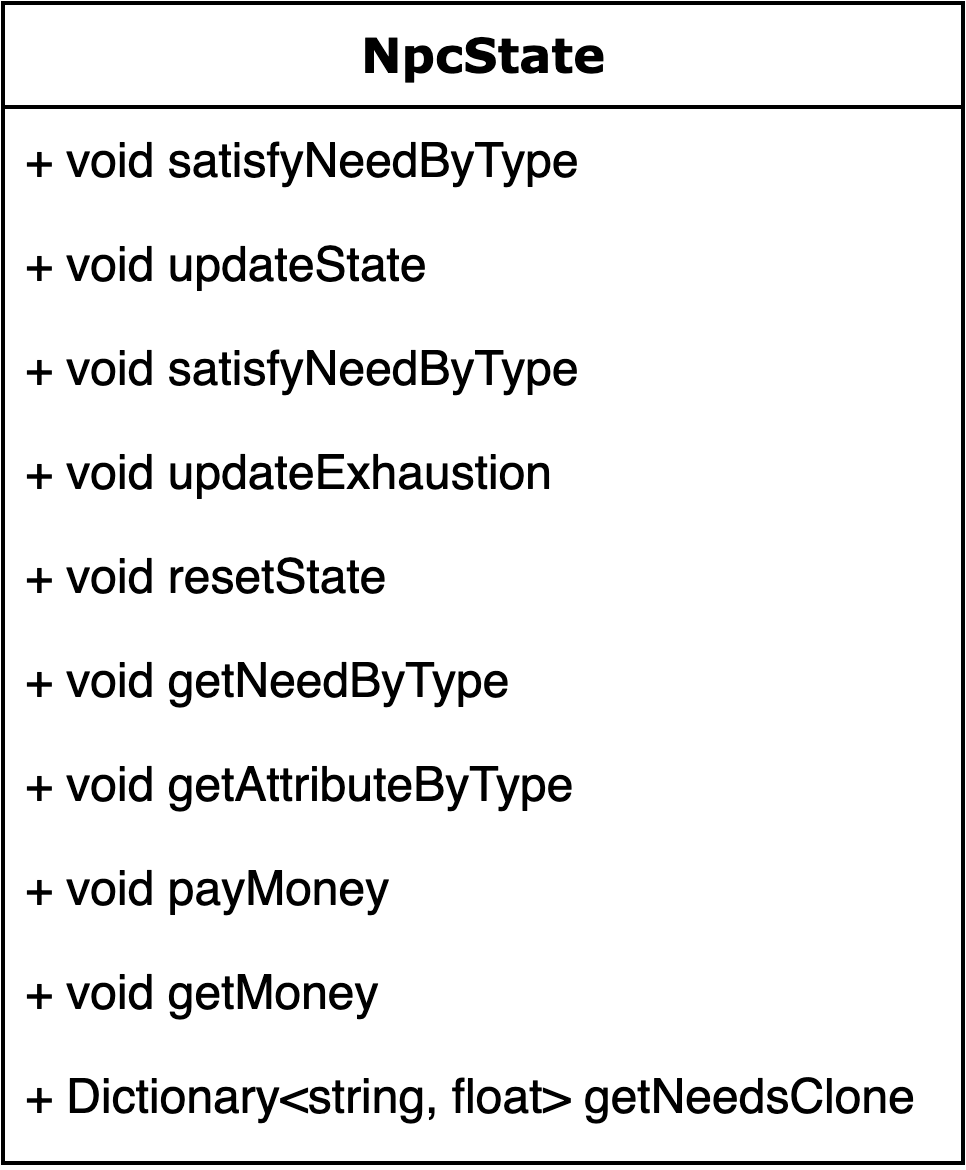
\includegraphics[scale=0.18]{images/village/architecture_diagram_npcstate.png}
\caption{Methoden der Klasse \inlinecode{WaitHandler}}
\label{fig:architecture_diagram_npcstate}
\end{figure}

Die Methoden \inlinecode{payMoney} und \inlinecode{gainMoney} werden genutzt, um die Geldmenge des Agenten zu verändern, beispielsweise wenn eine Aktion als Voraussetzung gewisse Kosten erfordert. Zusätzlich zu den im \inlinecode{ResourceHandler} definierten Ressourcen verfügt der Agent über eine spezielle Ressource \Fachbegriff{Money}, die im \inlinecode{NpcState} definiert wird. Im Gegensatz zu normalen Ressourcen verfügt jeder Agent über einen individuellen Wert für die Geldmenge, die er besitzt. Bestimmte Aktionen sind mit Kosten verbunden, die der Agent bezahlen muss. Geld kann nur durch Arbeits-Aktionen dazugewonnen werden. In einem ActionPlan kann durch die Veränderung der Variable \inlinecode{\_money} ein Wert für die Kosten der Aktion gesetzt werden. Dadurch soll der Agent über den Reward hinaus dazu angeregt werden, zu arbeiten. Außerdem führt dies dazu, dass bestimmte teure Aktionen von bestimmten Bevölkerungsgruppen, die mehr Geld verdienen, bevorzugt werden. Ein Bäcker verdient beispielsweise mehr Geld als ein Bauer.


Es werden einige Funktionen definiert, um Bedürfnisse und Attribute zu aktualisieren und abzufragen. In der Funktion \inlinecode{resetState} findet weiterhin nach dem Abschließen einer Episode ein Zurücksetzen der Werte statt. Da für die verteilte Belohnung in ActionPlans die initialen Bedürfnisse bekannt sind wurde die Funktion \inlinecode{getNeedsClone} implementiert. Sie gibt eine Kopie der aktuellen Werte aller Bedürfnisse zurück, die zu Beginn der Ausführung eines ActionPlans bezogen werden und nach der Ausführung verwendet werden kann.
Die Funktion \inlinecode{updateState} wird vom \inlinecode{TimeController} in regelmäßigen Abständen aufgerufen. Sie aktualisiert den Zustand des Agenten durch die Bereitstellung der neuen aktuellen Zeit und verändert damit seine Bedürfnisse. Die Funktion ist in Abbildung \ref{lst:npcstate_updatestate} zu sehen:

\begin{minipage}{\linewidth}
\begin{lstlisting}[linewidth=16.4cm, label=lst:npcstate_updatestate, caption=Funktion \inlinecode{updateState} in \inlinecode{NpcState}, xleftmargin=1cm, basicstyle=\footnotesize]
public void updateState(float currentTime, float deltaTime) {
    _exhaustion += 0.0002f * deltaTime;

    List<string> needsToUpdate = new List<string>();
    foreach (string needType in _needs.Keys) needsToUpdate.Add(needType);
    foreach (string needType in needsToUpdate) {
        _secondsSinceSatisfaction[needType] += deltaTime;
        _needs[needType] = _needCycleHandler.getUpdatedNeedValue(needType, _secondsSinceSatisfaction[needType]);
        if (_useGoap && _needs[needType] < 0.1f) _goapEffectSetter.setGoapEffect(needType, true);
    }
    _recreation = _needCycleHandler.calculateRecreationValue(_needs);
    _sleep = _needCycleHandler.calculateSleepValue(currentTime);
    _work = _needCycleHandler.calculateWorkValue(currentTime);
}
\end{lstlisting}
\end{minipage}

Neben den Werten für Exhaustion und Recreation (siehe Kapitel \ref{npc_needs_architecture}) werden ebenfalls die Bedürfnisse des Agenten angepasst, indem zusätzliche Funktionen aufgerufen werden. Die Bedürfnisse Schlaf und Arbeit werden dabei gesondert behandelt. Die genaue Funktionsweise der Bedürfnisse wird im folgenden Abschnitt \ref{npc_needs_architecture} behandelt.


\subsubsection{Bedürfnisse}\label{npc_needs_architecture}
Für die Simulationen werden Utility-Based Agents verwendet (siehe Abschnitt \ref{utility_agents}). Konkret werden diese so implementiert, dass sie über verschiedene menschliche Bedürfnisse verfügen. Im \inlinecode{NeedCycleHandler} werden jeweils Funktionen $g_b(x)$ definiert, die diese Bedürfnisse in Abhängigkeit von der verstrichenen Zeit verändern.

Ein Bedürfniswert von $g_b(x) = 1$ bedeutet, dass der Agent hinsichtlich dieses spezifischen Begehrens vollkommen befriedigt ist. Ein Bedürfniswert von $g_b(x) = 0$ hingegen bedeutet, dass der Agent ein starkes Bedürfnis hat, das es zu befriedigen gilt.
Als Grundbedürfnisse werden \textit{Hunger}, \textit{Durst}, \textit{Bildung}, \textit{Kommunikation}, und \textit{Glauben} definiert. Weiterhin gibt es die Bedürfnisse \textit{Schlaf} und \textit{Arbeit}. Im Spiel werden diese als \textit{NEED\_HUNGER}, \textit{NEED\_THIRST}, \textit{NEED\_EDUCATION}, \textit{NEED\_COMMUNICATION}, \textit{NEED\_FAITH}, \textit{SLEEP} und \textit{WORK} implementiert.

Die Werte für die fünf Grundbedürfnisse hängen davon ab, wann das Bedürfnis zuletzt befriedigt wurde. Sie verwenden die folgende Grundfunktion $g_b(x)$:

\begin{minipage}{\linewidth}
\begin{lstlisting}[linewidth=16.4cm, label=lst:village_needs_base_function, caption=Grundfunktion für die Abnahme der Grundbedürfnisse, xleftmargin=1cm]
private float _getFunctionValue(float cycleLengthSeconds, float exponent, float xValue) {
    float baseVal = xValue / cycleLengthSeconds;
    float pow = Mathf.Pow(baseVal, exponent);
    return Mathf.Clamp(1f - pow, 0f, 1f);
}
\end{lstlisting}
\end{minipage}

Für jede der Basisfunktionen $g_b(x)$ werden die in der Grundfunktion verwendeten Parameter wie \inlinecode{exponent}, \inlinecode{baseVal} und \inlinecode{cycleLengthSeconds} eigens definiert. Wenn die Bedürfnisse akutalisiert werden, wird für die Berechnung der einzelnen Werte ein \Fachbegriff{Switch-Case}-Konstrukt verwendet, wie in Listing \ref{lst:village_needs_switchcase} zu sehen.

\begin{minipage}{\linewidth}
\begin{lstlisting}[linewidth=16.4cm, label=lst:village_needs_switchcase, caption=Aufruf der Grundfunktion bei einer Anpassung der Bedürfnisse, xleftmargin=1cm]
public float getUpdatedNeedValue(string needType, float timeSinceSatisfaction) {
    switch(needType) {
        case NpcState.NEED_HUNGER:
            return _getFunctionValue(HUNGER_CYCLE_SECONDS,
                HUNGER_DROP_RATE, timeSinceSatisfaction);
        case NpcState.NEED_THIRST:
            return _getFunctionValue(THIRST_CYCLE_SECONDS,
                THIRST_DROP_RATE, timeSinceSatisfaction);
        [...] // Cases with other needs.
    }
    return -1f;
}
\end{lstlisting}
\end{minipage}


Das folgende Beispiel betrachtet exemplarisch die Hungerfunktion $g_{hunger}(x)$ des Agenten. Wenn die verwendeten Konstanten eingesetzt werden, ergibt sich der folgende Aufruf:

\begin{minipage}{\linewidth}
\begin{lstlisting}[linewidth=16.4cm, label=lst:village_needs_hunger_call, caption=Aufruf der Grundfunktion bei einer Anpassung der Bedürfnisse, xleftmargin=1cm]
_getFunctionValue(
    cycleLengthSeconds = DAY_CYCLE_SECONDS * 0.5f,
    exponent = 2.5f,
    xValue = timeSinceSatisfaction
);
\end{lstlisting}
\end{minipage}

Durch Einsetzen der Werte verändert das die Grundfunktion wie folgt:

\begin{minipage}{\linewidth}
\begin{lstlisting}[linewidth=16.4cm, label=lst:village_needs_base_function_eingesetzt, caption=Grundfunktion für Bedürfnisse (Beispiel Hungerbedürfnis), xleftmargin=1cm]
float baseVal = timeSinceSatisfaction / (DAY_CYCLE_SECONDS * 0.5f);
float pow = Mathf.Pow(baseVal, 2.5f);
return Mathf.Clamp(1f - pow, 0f, 1f);
\end{lstlisting}
\end{minipage}

Nun ist leicht zu sehen, dass sich folgende mathematische Funktion daraus ergibt: 

$$ g_{hunger}(x) = 1 - {(x / 500)}^2.5 $$

Die Funktionen für das Schlaf- und Arbeitsbedürfnis wurden anhand von Abbildung \ref{fig:village_diagram_hunger-function} visualisiert. Für die Variable \inlinecode{DAY\_CYCLE\_SECONDS}, die den Tageszyklus bestimmt. wird dabei eine Dauer von 1000 Sekunden genutzt.

\begin{figure}[H]
\centering
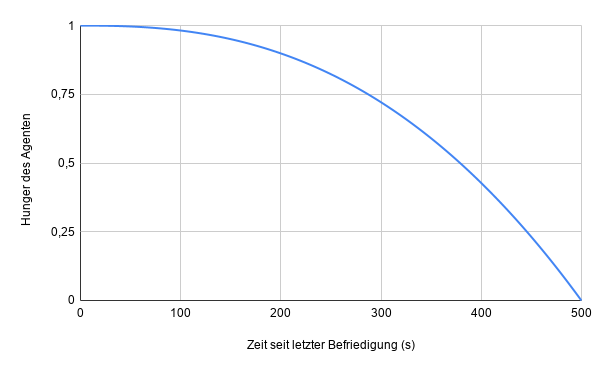
\includegraphics[scale=0.7]{images/village/village_diagram_hunger-function.png}
\caption{Hungerfunktion des Agenten}
\label{fig:village_diagram_hunger-function}
\end{figure}

Die Bedürfnisse \Fachbegriff{Schlaf} und \Fachbegriff{Arbeit} verhalten sich anders. Diese sind nicht davon abhängig, wann das Bedürfnis das letzte mal befriedigt wurde, sondern hängen von der Tageszeit ab. Das Listing \ref{lst:village_sleep_function} zeigt, wie das Schlafbedürfnis berechnet wird.

\begin{minipage}{\linewidth}
\begin{lstlisting}[linewidth=16.4cm, label=lst:village_sleep_function, caption=Funktion für das Schlafbedürfnis, xleftmargin=1cm]
public float calculateSleepValue(float currentTime) {
    float baseOffsetX = -0.125f;

    bool exceedsBorders = _exceedsBorders(0.125f - baseOffsetX, 0.625f - baseOffsetX, currentTime);
    if (!exceedsBorders) return 1f;

    float frequency = 4f * Mathf.PI;
    float offset = currentTime + baseOffsetX;
    float funcRes = Mathf.Sin(frequency * offset) * 0.5f + 0.5f;
    return Mathf.Clamp(funcRes, 0f, 1f);
}
\end{lstlisting}
\end{minipage}

Daraus ergibt sich folgende Funktion:

$$ g_{sleep}(x) =  \sin{(4 \pi * (x - 0.125))} * 0.5 + 0.5  $$

Diese Funktionen werden als Basis für eine partielle Funktion verwendet. Die Funktion \inlinecode{\_exceedsBorders} prüft, ob die Werte der X-Achse bestimmte Grenzen überschreiten. Falls dies der Fall ist, wird der Funktionswert nicht durch die oben definierten Funktionen berechnet, sondern entspricht automatisch dem Wert $1$. Die Intervalle, die diese Grenzen für das Schlaf- und Arbeitsbedürfnis definieren, heißen $I_{sleep}$ bzw. $I_{work}$.

$$ g_{sleep}(x)= \left\{
    \begin{array}{ll}
        x \in I_{sleep},     \;\;\;     \sin{(4 \pi * (x - 0.125))} * 0.5 + 0.5     \\
        x \not\in I_{sleep}, \;\;\;   1
    \end{array}
\right.  $$

Die Berechnung des Arbeitsbedürfnis verläuft auf die gleiche Art und Weise. Hier wird lediglich der Offset in der Funktion anders berechnet, wie in Listing \ref{lst:village_work_function_offset} zu sehen. In das Offset wird die Schlafdauer des Agenten mit einbezogen und ein zusätzliches Offset einberechnet. Der Agent soll idealerweise morgens aufwachen und nach kurzer Zeit einen Zuwachs seines Arbeitsbedürfnisses verspüren.

\begin{minipage}{\linewidth}
\begin{lstlisting}[linewidth=16.4cm, label=lst:village_work_function_offset, caption=Berechnung des Offset für das Arbeitsbedürfnis, xleftmargin=1cm]
float sleepDuration = SleepActionPlan.SLEEP_DURATION_HOURS / 24f;
float baseOffsetX = -0.125f - sleepDuration - WORK_SLEEP_OFFSET;
\end{lstlisting}
\end{minipage}

Für das Arbeitsbedürfnis ergibt sich folgende Funktion:

$$ g_{work}(x)= \left\{
    \begin{array}{ll}
        x \in I_{work},     \;\;\;     \sin{(4 \pi * (x - O_{sw}))} * 0.5 + 0.5     \\
        x \not\in I_{work}, \;\;\;   0
    \end{array}
\right.  $$
\begin{centering}  wobei $ O_{sw} = -0.125f - sleepDuration - WORK\_SLEEP\_OFFSET $  \end{centering}
\bigskip

$O_{sw}$ beschreibt den Offset zwischen Werten der Schlaf- und der Arbeitsfunktion.
$g_{work}(x)$ und $g_{sleep}(x)$ können nun berechnet werden. Sie können in Abbildung \ref{fig:village_diagram_sleep_work_functions} betrachtet werden.

\begin{figure}[H]
\centering
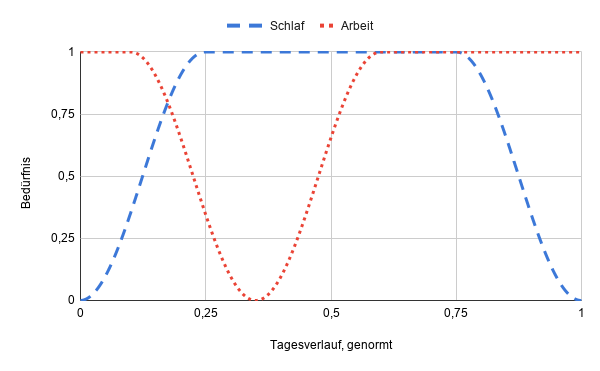
\includegraphics[scale=0.7]{images/village/village_diagram_work_sleep_functions.png}
\caption{Bedürfnisfunktionen des Agenten für Arbeit und Schlaf}
\label{fig:village_diagram_sleep_work_functions}
\end{figure}


Für die Berechnung der Schlaf- und Arbeitsfunktion wird weiterhin ein für jeden Agenten unterschiedlicher Wert verwendet. Bei der Initialisierung des Agenten wird dem Feld \inlinecode{\_rythmVariation} ein zufälliger Wert zugewiesen, um jedem Agenten einen leicht versetzten Rhytmus zu verleihen. Die maximale Amplitude dieses Werts kann durch eine Anpassung der Variable \inlinecode{agentRythmVariation} in der Klasse \inlinecode{GameAcademy} gesteuert werden. Ohne disen OFfset kann es dazu kommen, dass viele - oder alle - Agenten zur selben Zeit schlafen bzw. arbeiten gehen und sich identische Tagesabläufe abbilden.

Zusätzlich zu den genannten Bedürfnissen wurden ein \Fachbegriff{Recreation}-Wert und ein \Fachbegriff{Exhaustion} eingeführt. Der Recreation-Wert ist für das Auslösen von Freizeitaktivitäten verantwortlich. Er berechnet sich wie folgt:

\begin{minipage}{\linewidth}
\begin{lstlisting}[linewidth=16.4cm, label=lst:village_recreation_function, caption=Berechnung des Recreationwerts, xleftmargin=1cm]
public float calculateRecreationValue(Dictionary<string, float> needs) {
    float recreationValue = 0f;
    foreach (string needType in needs.Keys)
    {
        float need = needs[needType];
        if (need < BaseActionPlan.NEED_PENALTY_THRESHOLD) recreationValue += (1f - need) * 100;
        else if (need < 0.3f) recreationValue += (1f - need) * 10f;
        else if (need < 0.4f) recreationValue += (1f - need) * 3f;
        else recreationValue += 1f - need;
    }
    recreationValue = recreationValue / needs.Count / 1.5f;
    return Mathf.Clamp(recreationValue, 0f, 1f);
}
\end{lstlisting}
\end{minipage}

Recreation ist also abhängig von allen Grundbedürfnissen des Agenten. Je \sogenannt{glücklicher} ein Agent ist, also je höher die Werte seiner Grundbedürfnisse sind, desto niedriger ist der Recreationwert. Sobald ein Agent hinsichtlich all seiner Bedürfnisse befriedigt ist, soll er durch einen dann niedrigen Recreationwert Freizeitaktivitäten nachgehen.

Exhaustion wird verwendet, um die Erschöpfung des Agenten zu simulieren. Der Exhaustionwert wird mit jeder \Fachbegriff{MoveAction} und durch das Arbeiten reduziert. Der Wert kann durch Ausruhen, Schlafen oder langes Warten wieder aufgefüllt werden.


\subsubsection{Navigation}\label{agent_navigation}
Während der \inlinecode{LocationHandler} für die Auswahl von Gebäuden zuständig ist und dahingehend Zielpositionen zur Verfügung stellt, ist der \inlinecode{MoveHandler} für die tatsächliche Navigation der Agenten verantwortlich. Dafür wird ein sogenannter \Fachbegriff{NavMeshAgent} verwendet \cite{unity_navmeshagent}. Es handelt sich dabei um ein Feature, das lediglich in der kommerziellen Pro-Version von Unity nutzbar ist. Der \Fachbegriff{NavMeshAgent} nutzt ein \Fachbegriff{NavMesh}, das vorher generiert werden muss. Die Vorberechnung des NavMesh nennt sich \Fachbegriff{Baking}. Das NavMesh ist eine abstrakte Datenstruktur aus zweidimensionalen Polygonen, die für die Wegfindung des Agenten genutzt wird \cite{unity_navmesh}. Es definiert Flächen, die von einem Agenten traversiert werden können. Um Wege zwischen den Polygonen des NavMesh zu finden, können klassische Pathfinding-Algorithmen wie A* verwendet werden. Durch die Verwendung performanter Algorithmen und der Vorberechnung des NavMesh verläuft das Pathfinding sehr effektiv. Im weiteren Verlauf wird angenommen, dass das gesamte NavMesh in der Simulation statisch ist. Kollisionen von Agenten mit der Umgebung kommen daher nicht vor. Weiterhin werden Kollisionen von Agenten untereinander ignoriert.

\begin{figure}[H]
\centering
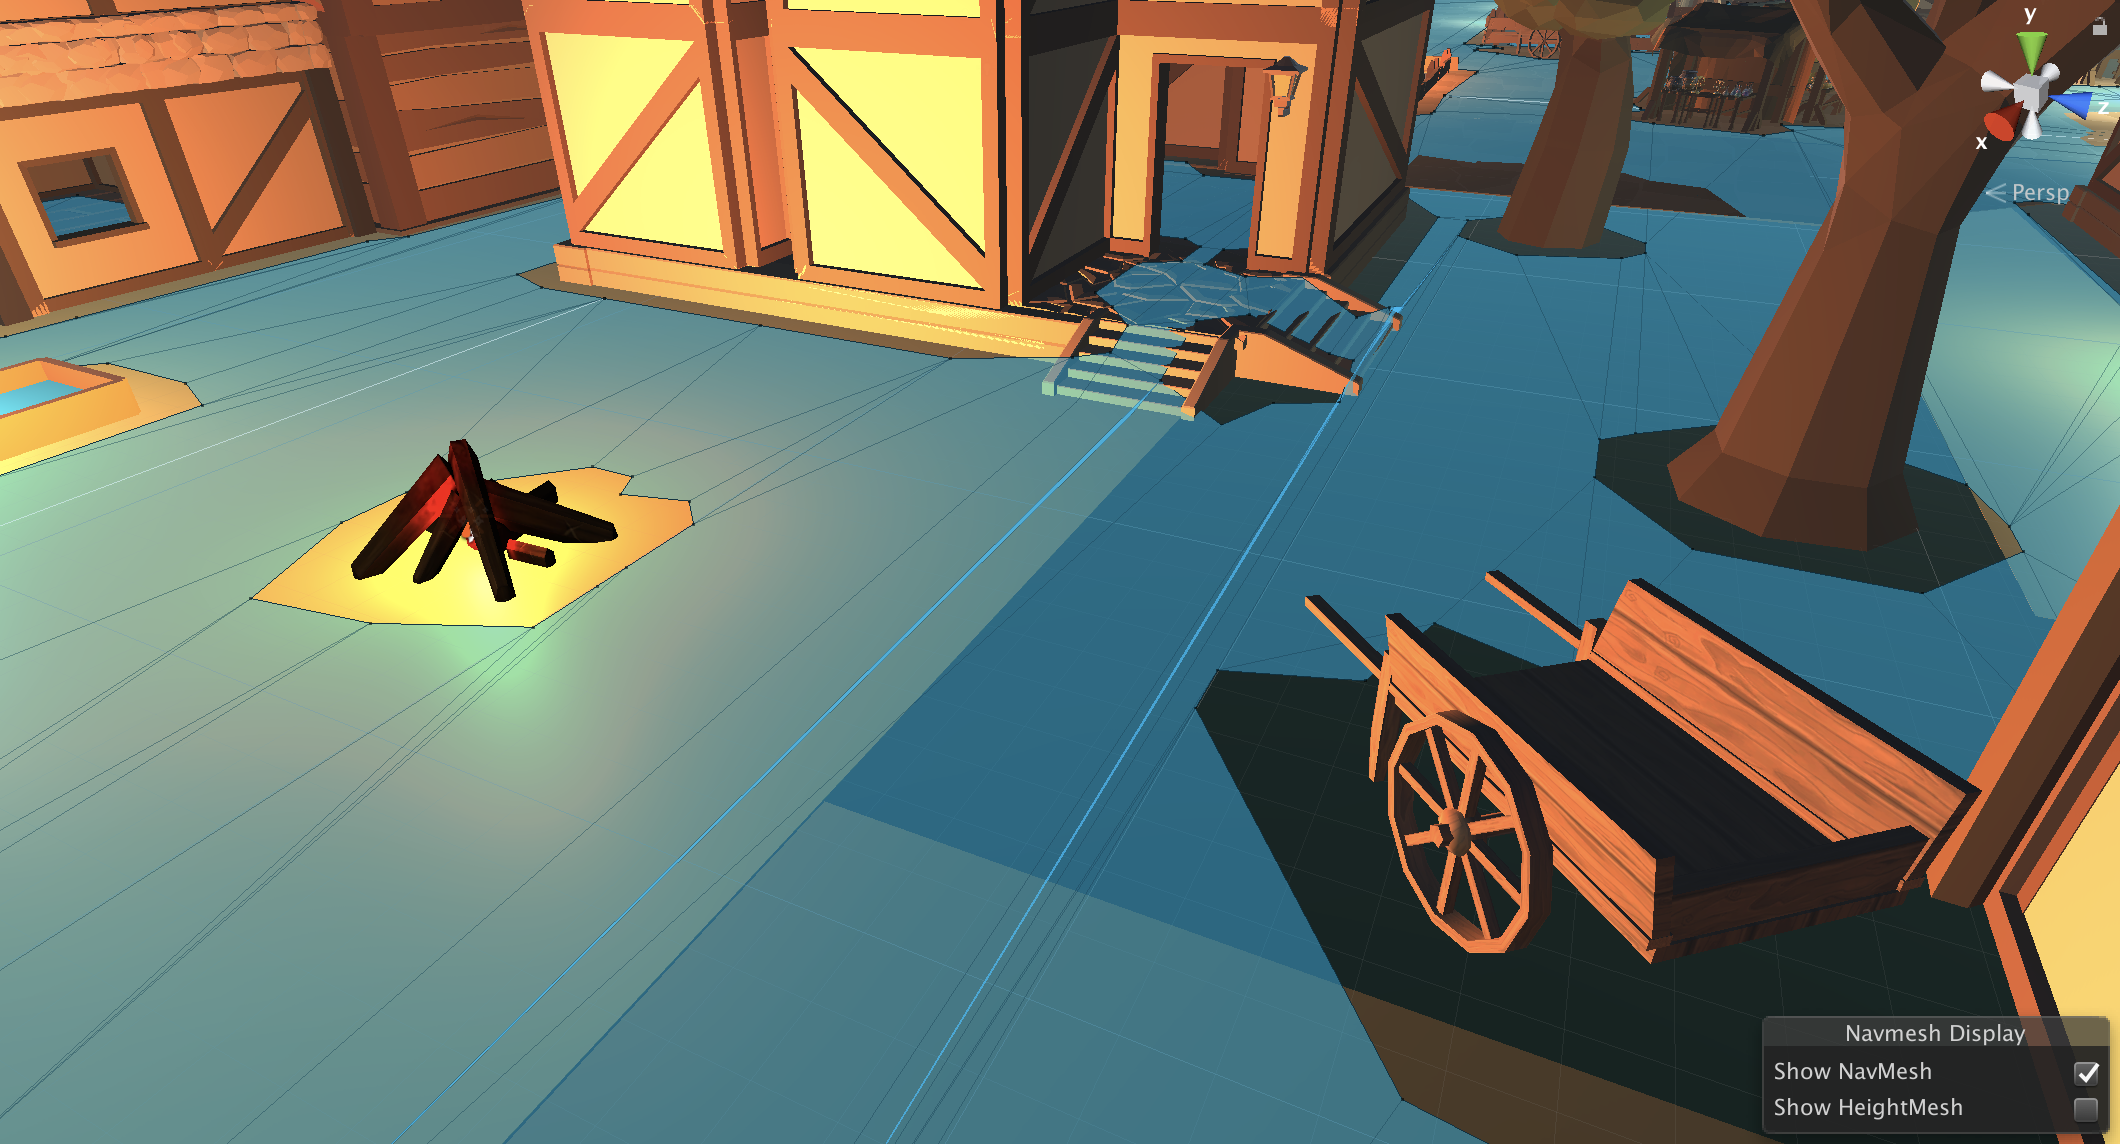
\includegraphics[scale=0.4]{images/village/village_navmesh_1.png}
\caption{Beispielhafter Ausschnitt des generierten NavMesh}
\label{fig:village_navmesh_1}
\end{figure}

Abbildung \ref{fig:village_navmesh_1} zeigt einen beispielhaften Ausschnitt aus dem für die Dorfsimulation generierten NavMesh. Auf der Abbildung ist gut zu erkennen, dass nicht-begehbare Objekte das NavMesh unterbrechen. Beispielsweise bilden der Karren im Vordergrund sowie die Bäume, die Häuser oder das Lagerfeuer Einschnitte in das NavMesh.
Um das NavMesh zu erzeugen, muss für Objekte gekennzeichnet werden, ob sie in die Berechnung mit einbezogen werden oder nicht. Für die Generierung müssen weiterhin einige Parameter gesetzt werden, die die Maße des Agenten beschreiben, sodass Abstände korrekt berücksichtigt werden. Außerdem muss festgelegt werden, wie hoch der Agent springen und welche Steigungen er überwinden kann. Im hinteren Teil der Abbildung \ref{fig:village_navmesh_1} ist dies anhand der Treppe gut zu erkennen. Das blaue NavMesh liegt ebenfalls über der Treppe, weil ihre Steigung vergleichsweise gering ist, sodass der Agent sie ohne weiteres erklimmen kann. Für die Berechnung des NavMesh wurde die Voxelgröße auf 0,125 festgelegt, was bei einem Agentenradius von 0,6 Einheiten 4,8 Voxeln pro Agentenradius entspricht. Dieser Parameter steuert effektiv die Auflösung des NavMesh. Bei der gewählten Größe benötigt die Berechnung, bzw. der \Fachbegriff{Baking}-Vorgang, für ein einzelnes Dorf etwa 30 Sekunden. Um das NavMesh zu nutzen, muss nach erfolgreicher Generierung des NavMesh die Komponente NavMeshAgent an den zu steuernden Agenten angefügt werden. Eine Menge von Einstellungen wie die Geschwindigkeit und Beschleunigung des Agenten können darin gewählt werden.

Der \inlinecode{MoveHandler} hat die Aufgabe, dem NavMeshAgent ein Ziel zu geben. Über die Funktion \inlinecode{moveAgent}, welche als Parameter unter anderem eine Zielposition erhält, wird ein Pfad zum ausgewählten Ziel berechnet und die Wegfindung des Agenten gestartet. Für jeden neuen Frame prüft anschließend die Update-Methode der Klasse, ob das Ziel des Agenten erreicht wurde. Sobald dies der Fall ist wird eine Callbackfunktion aufgerufen, welche die Move-Aktion des Agenten abschließt und die nächste auszuführende Aktion des entsprechenden ActionPlans startet. Die Abbildung \ref{fig:village_navmesh_2} zeigt einige Agenten, die über das NavMesh navigieren.

\begin{figure}[H]
\centering
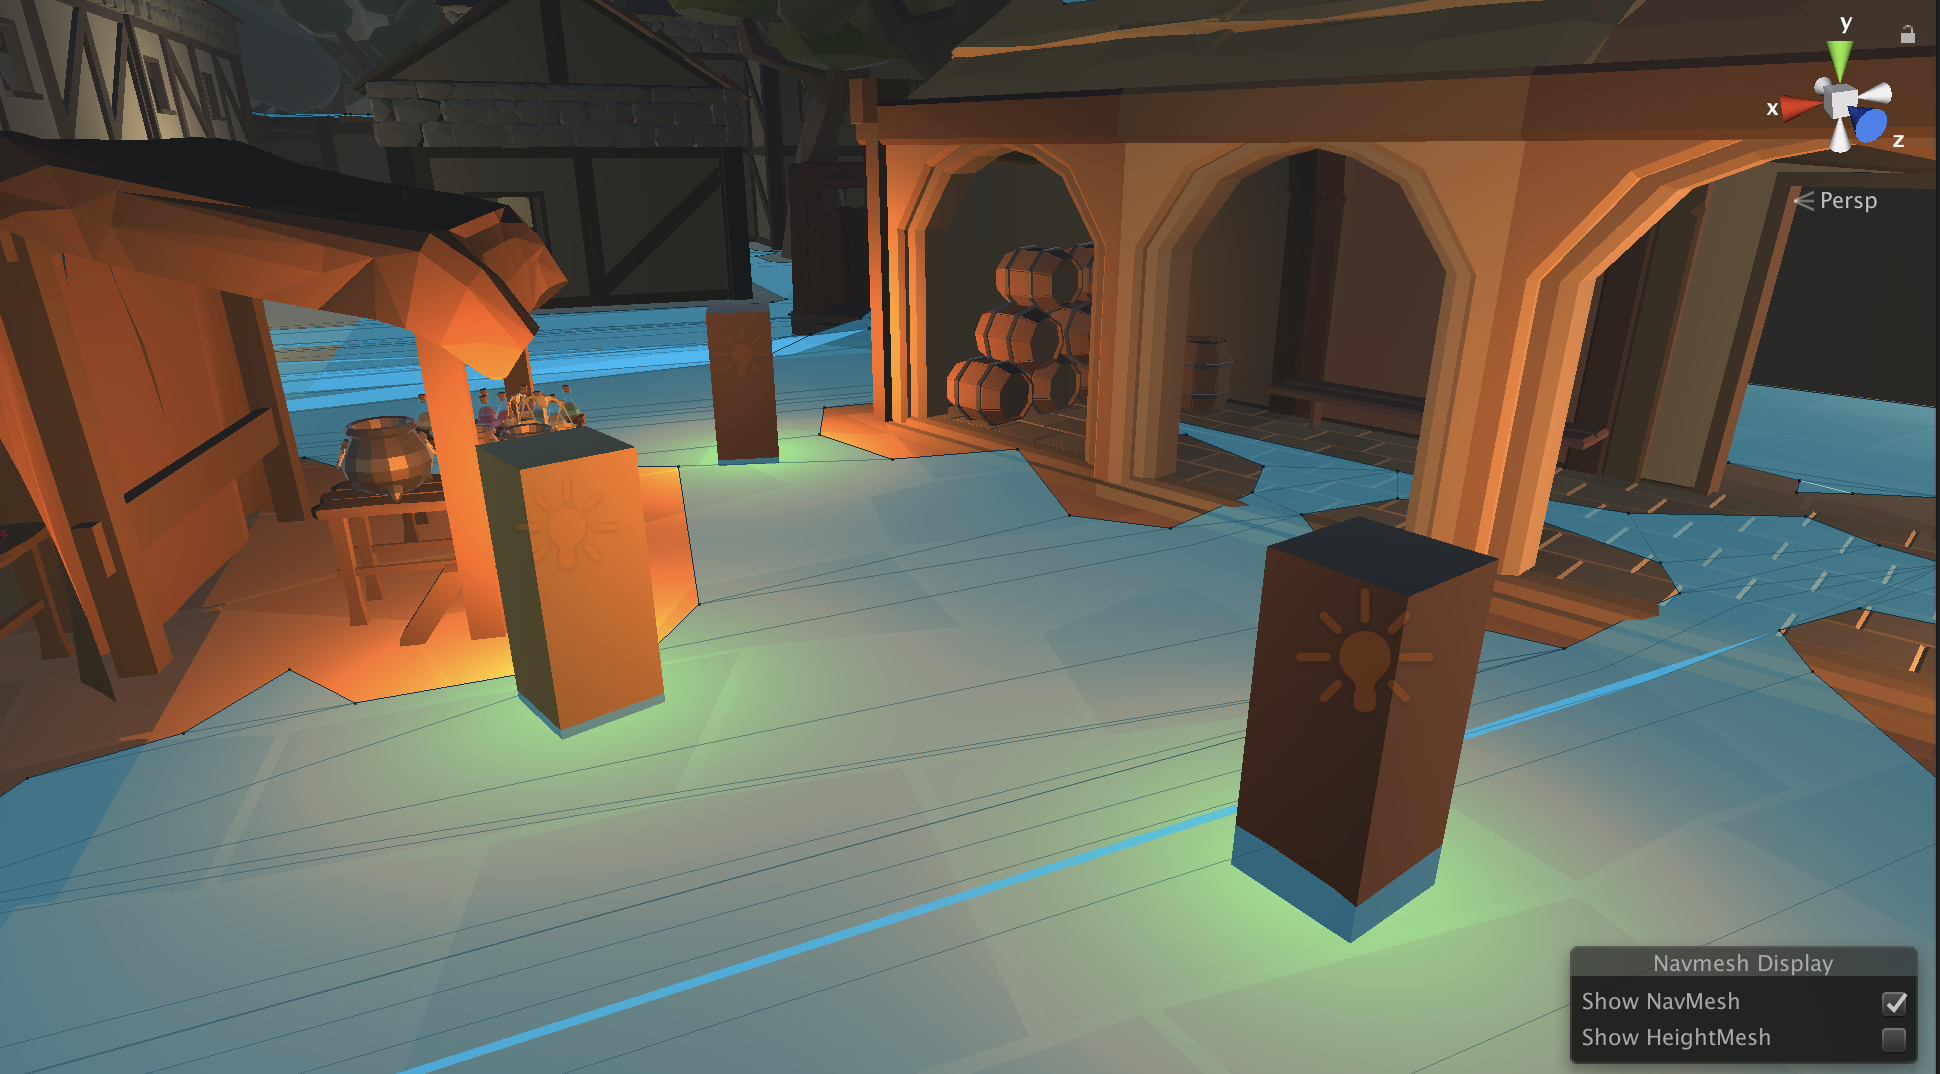
\includegraphics[scale=0.4]{images/village/village_navmesh_2.png}
\caption{Agenten navigieren über das NavMesh}
\label{fig:village_navmesh_2}
\end{figure}


\subsubsection{Maskieren von Aktionen}
Die Größe des Aktionsraum des Agenten ändert sich mit dem Simulationszustand und den Parametern des Agenten. Nicht zu jeder Zeit sind alle Aktionen ausführbar. Stattdessen ist jeder ActionPlan, den der Agent ausführen kann, an bestimmte Bedingungen geknüpft. ML-Agents bietet die Möglichkeit, Aktionen zu \Fachbegriff{maskieren}. Das bedeutet, dass diese Aktionen bei der Entscheidungsfindung nicht in Erwägung gezogen werden. Das neuronale Netz liefert also garantiert einen Output, bei dem die maskierten Aktionen nicht gewählt werden.
Die Erzeugung der \Fachbegriff{ActionMask} ist im folgenden Listing \ref{lst:village_action_mask_creation} erkennbar.

\begin{minipage}{\linewidth}
\begin{lstlisting}[linewidth=16.4cm, label=lst:village_action_mask_creation, caption=Erzeugung der \Fachbegriff{ActionMask} für Aktionen, xleftmargin=1cm]
_actionMask = new List<string>();

foreach (string actionId in NpcActions.ALL_ACTIONS) {
    if (!_actionHandler.areRequirementsMet(actionId)) _actionMask.Add(actionId);
}
\end{lstlisting}
\end{minipage}

Im Abschnitt \ref{action_plans} wurde bereits beschrieben, wie Aktionen mit String-Identifiern verbunden werden. Die Maskierung wird im \inlinecode{ActionMaskingHandler} vorgenommen. Der Aufbau dieser Klasse ist in der folgenden Abbildung \ref{fig:architecture_diagram_actionmaskinghandler} zu erkennen:

\begin{figure}[H]
\centering
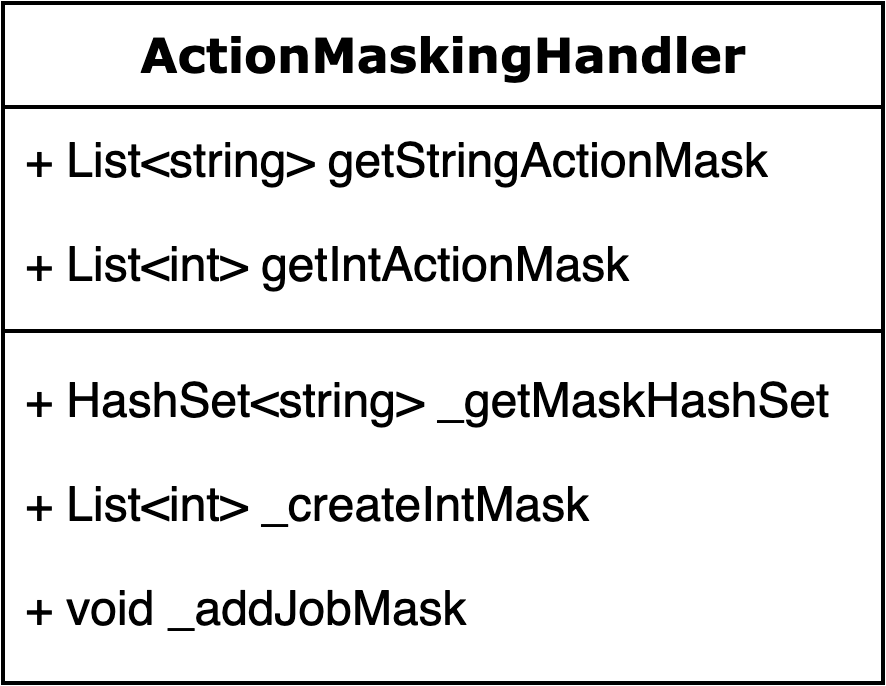
\includegraphics[scale=0.18]{images/village/architecture_diagram_actionmaskinghandler.png}
\caption{Methoden der Klasse \inlinecode{ActionMaskingHandler}}
\label{fig:architecture_diagram_actionmaskinghandler}
\end{figure}

Die eigentliche Erzeugung der ActionMask geschieht in der Funktion \inlinecode{\_getMaskHashSet}. Der \inlinecode{ActionMaskingHandler} iteriert dort über die Identifier aller möglichen Aktionen. Über den Identifier der Aktion erhält dieser vom \inlinecode{ActionHandler} den jeweiligen ActionPlan und ruft dessen Funktion \inlinecode{areRequirementsMet} auf. Wenn eine oder mehrere Bedingungen nicht zutreffen, wird die Aktion maskiert, sodass sie nicht ausgeführt wird. Es wird ein \inlinecode{HashSet<string>} verwendet, welches wie ein Dictionary funktioniert, in dem jedem Schlüssel nur ein einzelner Wert zugewiesen werden kann. Maskierte Aktionen können daher nur einmal in der Kollektion vorkommen - dies wird von ML-Agents gefordert.
Weiterhin wird für das Maskieren ein numerischer Identifier erwartet. Für spätere Verfahren werden hingegen Identifier in Form von \inlinecode{string}s erwartet. Daher wird ein umgekehrtes Mapping verwendet, das aus den String-Identifiern erneut numerische Identifier erzeugt. Weiterhin wird ein Wert vom Typ \inlinecode{List} statt \inlinecode{HashSet} erwartet. Für das Abfragen von integerbasierten oder stringbasierten ActionMasks gibt es daher die Funktionen \inlinecode{getStringActionMask} und \inlinecode{getIntActionMask}.


\subsubsection{Ausführungsfluss des Agenten}
Während der Durchführung von Aktionen interagiert der Agent mit einer Reihe verschiedener Komponenten. Die Architektur des Ausführungsflusses lässt sich anhand eines Komponentendiagramms beschreiben, wie in Abbildung \ref{fig:architektur_agent} zu sehen.

Das Diagramm dient als ergänzende Beschreibung zusätzlich zur generellen Architekturübersicht in Abbildung \ref{fig:architecture_general} und zeigt daher Gemeinsamkeiten. Hier wird jedoch mehr ins Detail gegangen und es besteht ein näherer Bezug zum Agenten selbst.

\bigskip
\begin{figure}[H]
\centering
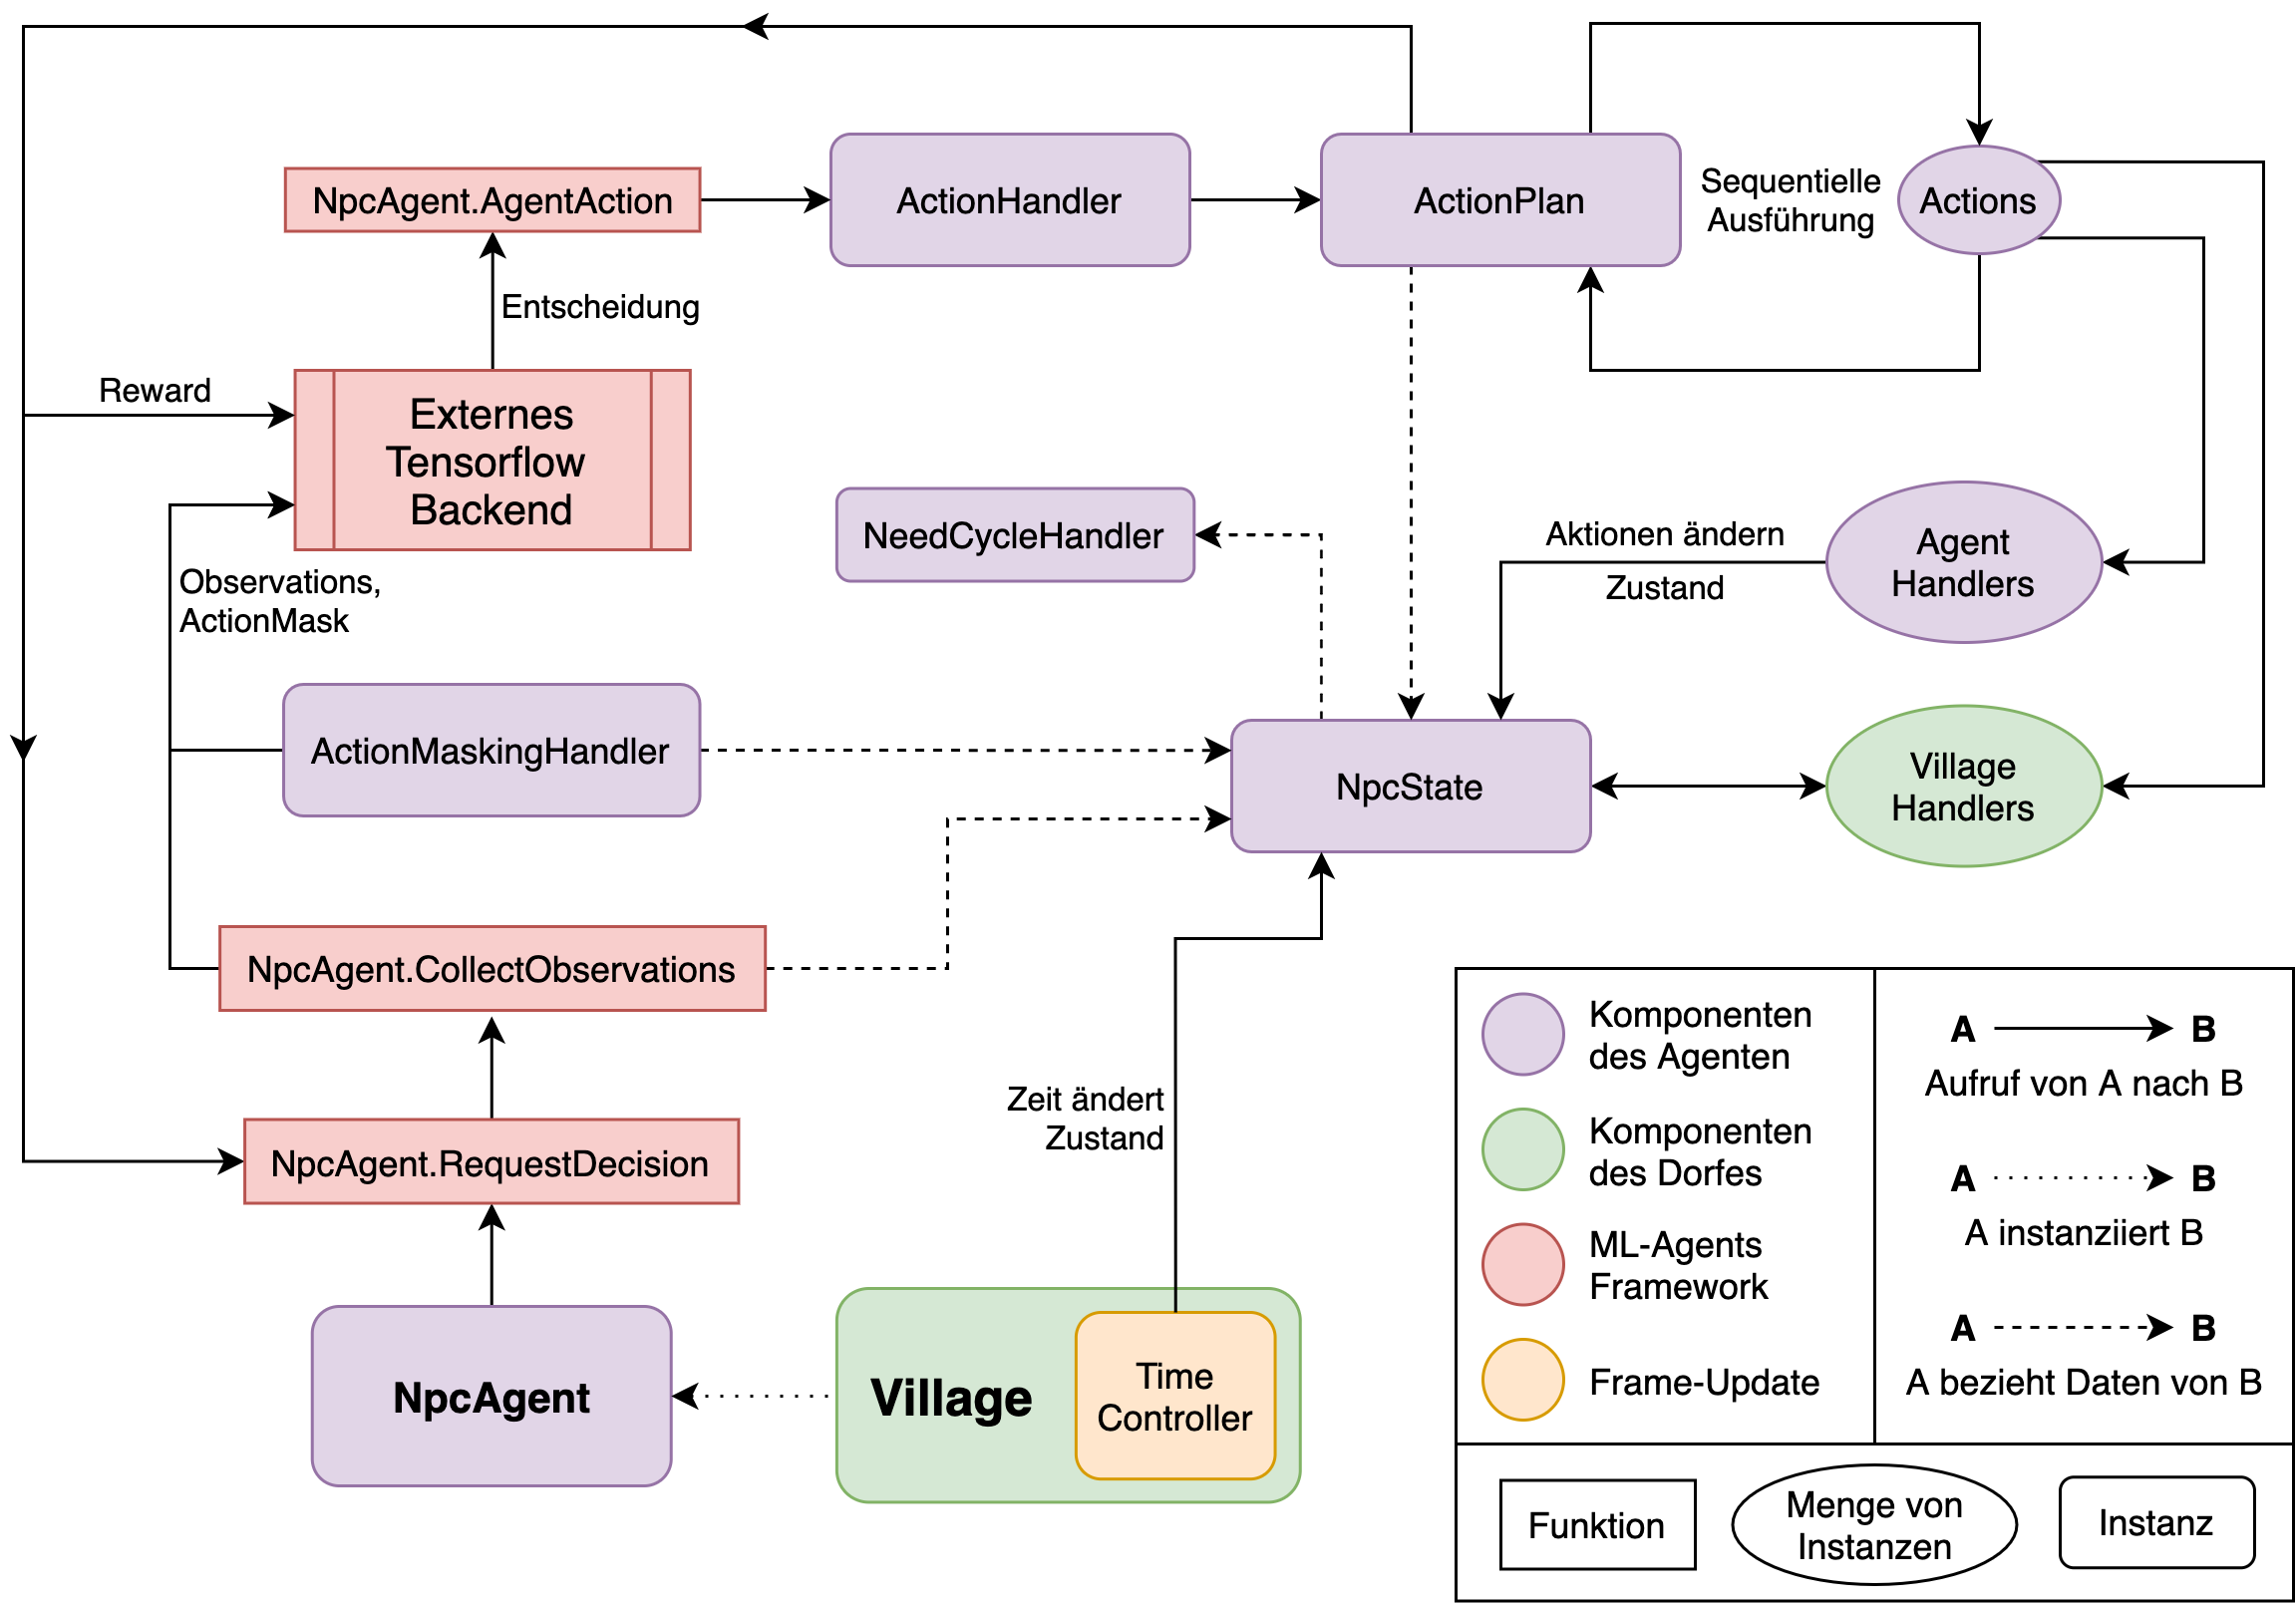
\includegraphics[scale=0.20]{images/village/Master-Thesis_Diagram_Architecture_3.png}
\caption{Architektur der Agenten}
\label{fig:architektur_agent}
\end{figure}

Als erstes sammelt der \ac{npc} eine Menge von Observations. Für die Observations wird der \inlinecode{NpcState} konsultiert. Weiterhin wird der \inlinecode{ActionMaskingHandler} aufgerufen, um den Aktionsraum zu begrenzen. ActionMask und Observations werden dann über die Verbindung des ML-Agents-Frameworks zum externen Tensforflow-Backend geschickt. Als Antwort darauf erhält der Agent eine neue Aktion. Die Funktion \inlinecode{AgentAction} wird aufgerufen und stellt die neue Aktion bereit. Diese wird durch den \inlinecode{ActionHandler} behandelt, der den entsprechenden ActionPlan bereitstellt. Nun werden die einzelnen Sub-Aktionen des ActionPlans ausgeführt. In der Regel sind das \Fachbegriff{Move}- und \Fachbegriff{Wait}-Aktionen. Weitere Aktionen werden in diesem Diagramm vernachlässigt. Die Move-Aktionen werden durch den \inlinecode{MoveHandler} ausgeführt, der mit dem \inlinecode{LocationHandler} kommuniziert. Der \inlinecode{WaitHandler} führt die Wait-Aktionen aus.
Wenn der Agent schließlich alle Sub-Aktionen ausgeführt hat, wird der \inlinecode{NpcState} aktualisiert. Aktionen haben Auswirkungen sowohl auf den Zustand des Agenten als auch unter Umständen auf den Zustand des Dorfes. Die neuen Bedürfnisse werden vom \inlinecode{NeedCycleHander} berechnet. Ressourcen werden aktualisiert und Bedürfnisse angepasst oder zurückgesetzt. Außerdem wird der \inlinecode{MonitorHandler} mit neuen Werten aus dem \inlinecode{NpcState} aktualisiert, um im HUD der Simulation aktuelle Werte anzuzeigen.
Außerdem wird eine Belohnung bzw. Bestrafung für die Aktion verteilt. Über eine Callbackfunktion im ActionPlan schließt sich der Ausführungskreislauf. Eine neue Aktion wird durch den Agenten gestartet, indem \inlinecode{RequestDecision} aufgerufen wird.
Zusätzlich zu diesem Ausführungsablauf wird in regelmäßigen Abständen die Update-Funktion der Komponente \inlinecode{TimeController} des Moduls \inlinecode{Village} aufgerufen, welche die Zustände aller Agenten verändert, indem sich durch das Voranschreiten der Zeit deren Bedürfnisse verändern.











\subsubsection{Belohnungen}\label{agents_rewards}
Die Belohnungen des Agenten hängen grundsätzlichen von seinen Bedürfnissen und dem Zweck der Aktion ab. Sie werden jeweils am Ende einer Aktionen verteilt und in den ActionPlans definiert. Jeder ActionPlan ist mit einem bestimmten Bedürfnis des Agenten verbunden, das durch ihn befriedigt wird. Die Berechnung der Belohnung berücksichtigt, wie ausgeprägt dieses bestimmte Bedürfnis zum Zeitpunkt der Ausführung war. Wenn der Agent beispielsweise sehr hungrig ist, also etwa einen Hungerwert $g_{hunger} = 0$ hat und eine Aktion \Fachbegriff{Essen} auswählt, welche das Hungergefühl stillt, so wird er eine hohe Belohnung bekommen. Wenn er bereits vollkommen gesättigt ist ($g_{hunger} = 1$) und die Aktion \Fachbegriff{Essen} auswählt, wird er eine Bestrafung erhalten. Der Agent soll dadurch lernen, Aktionen zu wählen, die seine Bedürfnisse sinnvoll befriedigen. Wenn alle Bedürfnisse befriedigt sind hat der Agent einen niedrigen Recreationwert, sodass er Freizeitaktivitäten nachgehen kann. Die Belohnungen funktionieren hier auf eine ähnliche Art und Weise. Dies ist ebenfalls beim Arbeits- und Schlafbedürfnis der Fall, obwohl diese Bedürfnisse nicht durch die Aktion aufgefüllt werden, sondern von der Tageszeit abhängen.


Die Belohnungen bestimmter Aktionen hängen außerdem von den Attributen der Agenten ab. Um den Agenten eine Persönlichkeit zu verleihen, werden Attribute wie \Fachbegriff{Intelligence}, \Fachbegriff{Companionship} oder \Fachbegriff{Fitness} im \inlinecode{NpcState} festgelegt.
Dadurch sollen allgemeine Unterschiede zwischen den Agenten, aber auch Unterschiede zwischen verschiedenen Gruppen von Agenten entstehen. Diese Gruppen werden durch die Berufe der Agenten bestimmt. Grundsätzlich werden die Attribute zufällig verliehen, zusätzlich wird bestimmten Berufen die Tendenz gegeben, bei bestimmten Attributen durchschnittlich höhere Werte zu erzielen als andere Berufe. Die Verleihung von Attributen aufgrund des Berufs spiegelt nicht die realen Welt, sondern wurde willkürlich festgelegt. Die Festlegung dieser Attribute wird in der statischen Klasse \inlinecode{AttributeHandler} durchgeführt. Die statische Methode \inlinecode{getAttributesByJobId} erhält als Parameter einen Identifier für den Job des Agenten und gibt ein \inlinecode{Dictionary<string,float>} mit den jeweiligen Attributen zurück. In einer \inlinecode{switch-case}-Anweisung werden die Attribute aufgrund des Berufs vergeben. Die Funktion wird vom \inlinecode{NpcState} aufgerufen.
Beispielsweise wird im ActionPlan \inlinecode{RecreationTavernActionPlan} eine Freizeitaktion definiert, die Agenten besuchen dabei die Taverne. Die Belohnung der Aktion skaliert invertiert mit dem Fitness- und Intelligenzlevel des \ac{npc}. Je niedriger die Fitness- und Intelligenzattribute des Agenten sind, desto höher fällt die Belohnung aus. So kommt es dazu, dass man mehr Minenarbeiter als Jäger in der Taverne antrifft, weil diese durchschnittlich über einen niedrigen Fitnesslevel sowie einen leicht niedrigeren Intelligenzlevel verfügen. Jäger werden mit einem überdurchschnittlich hohen Fitnesslevel häufiger auf dem Fußballplatz statt in der Taverne angetroffen. Beim Training werden diese Gegebenheiten durch die Veränderung des Rewards automatisch in den Lernvorgang mit einbezogen.

Für die Festlegung von Belohnung werden unter anderem die Hilfsfunktionen \inlinecode{\_getNeedReward}, \inlinecode{\_getRecreationReward}, \inlinecode{\_getNeedReward} der Klasse \inlinecode{BaseActionPlan} und die Funktion \inlinecode{\_getWorkReward} der Klasse \inlinecode{WorkActionPlan} verwendet. Mithilfe von Funktionen wie \inlinecode{\_calculateAttributeMultReward} werden Multiplikatoren für die Attribute berechnet, um die Belohnungen negativ oder positiv zu beeinflussen.
Weiterhin wird für sämtliche Belohnungen, die am Ende einer Aktion ausgeführt wurden, stets die Werte des Zustands des Agenten verwendet, die zum Anfang der Ausführung der Aktion vorhanden waren. Dadurch wird verhindert, dass der berechnete Reward direkt mit den vorher gesammelten Observations des Agenten übereinstimmen und eine Beziehung aufgebaut werden kann.











%  Der \inlinecode{JobHandler} ist unter anderem dafür zuständig, den Agenten in Abhängigkeit von den aktuell verfügbaren Ressourcen Berufe zuzuweisen.
\subsection{VillageAgent}\label{village_village_agent}
Den Agenten werden bei der Initialisierung Berufe zugewiesen. Für die Behandlung der Berufe der Agenten können mit der Anpassung des Parameters \inlinecode{ignoreJobMask} der Klasse \inlinecode{GameAcademy} zwei Modi gewählt werden. Der Parameter wurde eingeführt da sich beim Training herausgestellt hat, dass die Wahl der beruflichen Aktionen der Agenten eine Schwierigkeit darstellt.

Wenn der Parameter gesetzt ist wird der Beruf des Agenten ignoriert. Der Aktionsraum eines jeden Agenten verfügt dann über alle möglichen Berufsaktionen. Es wird also jeweils die berufliche Aktion gewählt, die für den Agenten voraussichtlich die höchste zukünftige Belohnung zuweist. Dadurch soll gewährleistet werden, dass das Ressourcensystem in einem stabilen Zustand gehalten wird, da das Ressourcenmanagement durch die Auswahl der beruflichen Aktivitäten der Agenten automatisch in einer Balance gehalten wird. Wenn von einer benötigte Ressource nur noch geringe Mengen vorhanden sind, sollten Agenten automatisch den Beruf ausführen, der die entsprechende Ressource herstellt. Die Agenten müssen in diesem Fall also Observations über die vorhandenen Ressourcen sammeln.    

Wenn der Parameter \inlinecode{ignoreJobMask} nicht gesetzt wird werden hingegen alle Jobs, die nicht dem Job des Agenten entsprechen, permanent maskiert und deren Ausführung dadurch blockiert. Der Agent hat dann also einen festen Job und wird von allen weiteren Jobs ausgeschlossen. Vor dem Trainingsvorgang ist allerdings nicht bekannt, wie viele Agenten welchen Job ausführen müssen, um eine Balance im Ressourcensystem herzustellen, wie oben beschrieben. Die Agenten müssen in diesem Fall keine Observations über die vorhandenen Ressourcen sammeln, da ohnehin keine Auswahl des Jobs möglich ist.    

Aus diesem Grund wird neben dem \inlinecode{NpcAgent} ein weiterer \ac{reinforcement_learning}-basierter Agent verwendet, der ML-Agents nutzt und sich darum kümmern soll, den Agenten in Abhängigkeit von den vorhandenen Ressourcen Jobs zuzuweisen. Die Implementierung ist in der Klasse \inlinecode{VillageAgent} zu finden. Die Aufgabe dieses Agenten ist es, den NPCs in Abhängigkeit von den vorhandenen Ressourcen in der Simulation Jobs zuzuweisen. Der Agent hat keinerlei visuelle Repräsentation im Spiel, sondern nimmt eine Art Beobachterrolle ein.
Nach einer gewissen Anzahl von Aktionen der Agenten wird durch die Academy automatisch eine neue Aktion des \inlinecode{VillageAgent} mittels \inlinecode{RequestDecision} gestartet. Der \inlinecode{VillageAgent} analysiert die Ressourcen und ermittelt, welche Ressource am wenigsten vorhanden ist. Weiterhin prüft er, welche Ressource am meisten vorhanden ist. Durch ein Mapping von den Ressourcen zu den dazugehörigen Jobs werden anschließend neue Jobs zugewiesen, wie in Listing \ref{lst:village_village_agent_actions} zu sehen. Der Agent verwendet anders als der \inlinecode{NpcAgent} insgesamt elf kontinuierliche Aktionen. Statt 24 diskreten, auswählbaren Aktionen wird hier für jede der elf Ressourcen immer ein kontinuierlicher Wert geliefert.

\begin{minipage}{\linewidth}
\begin{lstlisting}[linewidth=16.4cm, label=lst:village_village_agent_actions, caption=Aktionen des \inlinecode{VillageAgent}, xleftmargin=1cm]
public override void AgentAction(float[] vectorAction, string textAction) {
    float smallestValue = 1;
    int smallestIndex = -1;
    float largestValue = -1;
    int largestIndex = -1;
    for (int i = 0; i < vectorAction.Length; i++) {
        float value = vectorAction[i];
        if (value < smallestValue) {
            smallestValue = value;
            smallestIndex = i;
        } else if (value > largestValue) {
            largestValue = value;
            largestIndex = i;
        }
    }
    // Don't do anything, no change needed.
    if (largestValue < 0.3f && smallestValue > -0.3f) return; 

    string negJob = _indexToJob[smallestIndex];
    string negResource = _jobToResource[negJob];
    string posJob = _indexToJob[largestIndex];
    string posResource = _jobToResource[posJob];

    _assignNewWorkerJob(negJob, posJob);
    _addRewardsNew(negJob, posJob);
}
\end{lstlisting}
\end{minipage}

Wenn die Differenz groß genug ist, wird dem Beruf, der am meisten Ressourcen produziert hat, ein \inlinecode{NpcAgent} entzogen und dem Beruf, der am wenigsten produziert hat, hinzugefügt. So soll automatisch eine Balance gefunden werden, da die Berufe nicht alle gleich viele Ressourcen produzieren. Die kontinuierlichen Werte, die im Parameter \inlinecode{vectorAction} enthalten sind, beschreiben also, in welchen Berufen zu viele und in welchen Berufen zu wenige Agenten arbeiten.
Für die Belohnung des Agenten werden die durchschnittlichen Abweichungen der jeweiligen Ressourcen für den hinzugefügten und entfernten Job verwendet. Wenn einem Agent ein Job zugewiesen wird, in dem aktuell nur wenige Ressourcen vorhanden sind, so resultiert dies also in einer hohen Belohnung. Eine Zuweisung in einen Beruf mit bereits hohen verbundenen Ressourcenwerten resultiert in einer Bestrafung.
Der \inlinecode{VillageAgent} wird durch die Funktion \inlinecode{IncrementNumAgentActions} in der Klasse \inlinecode{GameAcademy} zurückgesetzt. Für jede Aktion eines Agenten wird diese Funktion aufgerufen und inkrementiert einen Zähler. Wenn dieser Zähler einen bestimmten Wert erreicht, der von den Parametern der \inlinecode{GameAcademy} abhängt, werden der \inlinecode{VillageAgent} und die Berufe aller Agenten zurückgesetzt. 







\subsection{UI}
Um Informationen zur Simulation an einem zentralen, leicht zugänglichen Ort anzeigen zu lassen, wurden verschiedene UI-Elemente entwickelt. Im Folgenden werden diese erläutert.

\paragraph{Dorfstatistiken}
Für das UI wird die Klasse \inlinecode{Monitor} aus dem ML-Agents Framework verwendet. Auf dieser Grundlage wurde eine eigene Klasse \inlinecode{GameMonitor} erstellt. Sie bietet eine einfache Möglichkeit, Informationen als UI-Elemente anzeigen zu lassen und erweitert die Klasse \inlinecode{Monitor} um einige anwendungsspezifische Funktionen. Bei den verwendeten UI-Elementen handelt es sich um Textelemente und Balken. Der visuelle Aspekt spielt hier keine wesentliche Rolle, sondern die Vermittlung von Informationen. Zusätzlich wurden in der Basisklasse \inlinecode{Monitor} einige Änderungen vorgenommen, um die Darstellung von Informationen anzupassen und für das zugrunde liegende Szenario zu verbessern.
Die nötigen Informationen werden in der Klasse \inlinecode{VillageInfo} gesammelt. Zum Beispiel wird immer dann, wenn ein Agent eine Aktion ausführt, ein entsprechender Zähler in der Klasse verändert. Im UI wird für alle möglichen Aktionen ein Textfeld eingeblendet, das die jeweilige Anzahl der Agenten beschreibt, die in diesem Moment die Aktion ausführen. Zusätzlich werden Werte wie Ressourcen und die aktuelle Zeit dargestellt.


\paragraph{Agentenspezifische Informationen}
Während der Ausführung der Simulation kann auf Agenten geklickt werden, um im UI agentenspezifische Informationen anzeigen zu lassen. Dafür muss eine bestimmte Kamera ausgewählt werden, die über die Komponente \inlinecode{OrbitCameraBehaviour} verfügt. Diese verfügt über ein Script, das eine Steuerung der Position und Rotation der Kamera über Tastatureingaben ermöglicht \cite{unity_camera_rotation_script}. Das Script wurde so modifiziert, dass es nun möglich ist, innerhalb der Simulation NPCs anzuklicken. Dieses Verhalten wird durch die Klasse \inlinecode{InteractionHandler} geregelt. Die Kamera wird dann mit dem Transform des Agenten verbunden, sodass diese ihm folgt und man die virtuelle Welt aus den Augen des NPCs betrachtet. Weiterhin wird in der Klasse \inlinecode{NpcAgent} der Boolsche Wert \inlinecode{\_shouldMonitor} gleich \inlinecode{true} gesetzt. Eine Instanz der Klasse \inlinecode{MonitorHandler} prüft in regelmäßigen Abständen den Zustand dieser Variable. Dadurch werden weitere UI-Elemente aktiviert, die für diesen spezifischen Agenten Informationen zu seinen Bedürfnissen, der aktuellen Aktion etc. anzeigt. Alternativ kann im Editor der Wert \inlinecode{\_shouldMonitor} für beliebige Agenten direkt beeinflusst werden, um bestimmte Informationen anzuzeigen. Jeder Agent besitzt die beiden Komponenten \inlinecode{MonitorHandler} und \inlinecode{InteractionHandler}.
In der Abbildung \ref{fig:village_ui_example_1} ist ein Beispiel für das im Spiel angezeigte UI aus der Perspektive eines Agenten erkennbar.

\begin{figure}[H]
\centering
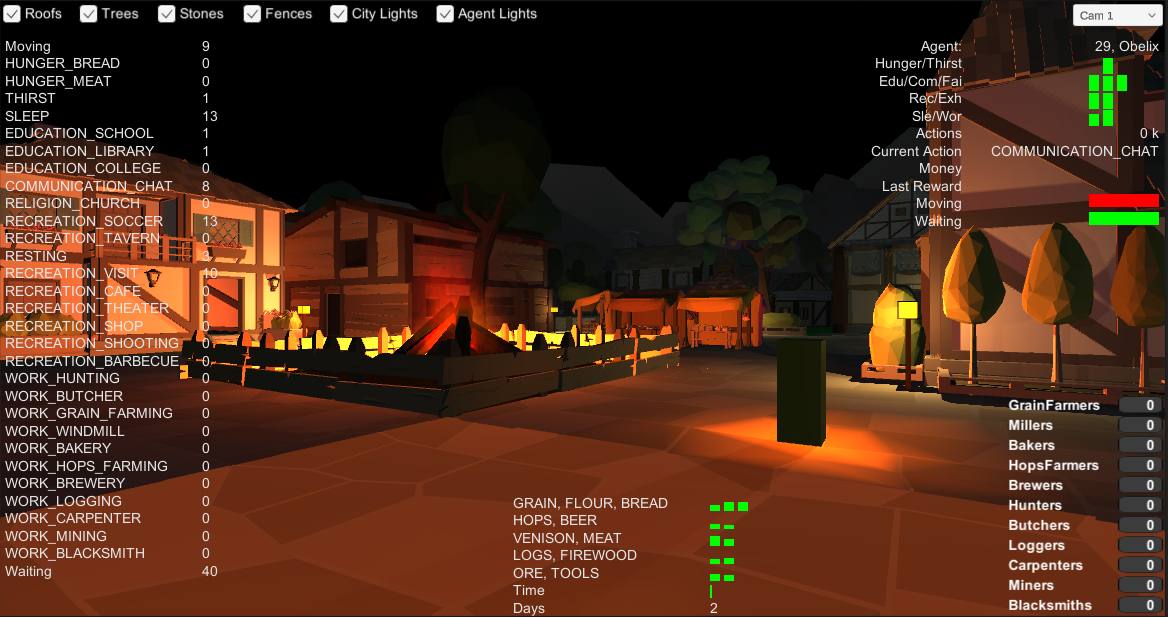
\includegraphics[scale=0.53]{images/village/village_ui_example_1.PNG}
\caption{UI aus Sicht eines Agenten}
\label{fig:village_ui_example_1}
\end{figure}

\paragraph{Anpassung der Szene}\label{szene_anpassung_ui}
Weiterhin wurden UI-Elemente entwickelt, um Anpassungen in der Szene vorzunehmen. Sämtliche Dächer der Gebäude im Dorf können über einen Agenten deaktiviert und aktiviert werden. Dadurch kann besser gesehen werden, wo die Agenten sich aufhalten. Zusätzlich können weitere Mesh-Elemente deaktiviert werden, um die Performance der Simulation zu erhöhen oder einen besseren Überblick zu bekommen. Konkret lässt sich das Mesh von Bäumen, Zäunen, Gebäuden und Felsen über einen Button deaktivieren. Zusätzlich können sämtliche Lichter in der Stadt deaktiviert werden. Dabei wird zwischen den Lichtquellen der Agenten und den Lichtquellen der Stadt unterschieden.
Weiterhin besteht die Möglichkeit, über einen Dropdown-Menü die Wahl der aktiven Kamera anzupassen. Dadurch kann ebenfalls die Spielerkamera aktiviert werden, sodass der \Fachbegriff{Player} gesteuert werden kann (siehe Abschnitt \ref{player}).
Diese Anpassungen werden in der Klasse \inlinecode{GameUI} vorgenommen. Die Klasse steuert die entsprechenden UI-Elemente bzw. nimmt Befehle von ihnen entgegen. Bei einer Verwendung mehrerer Dörfer wird nicht zwischen einzelnen Dörfern unterschieden. Die Änderungen treten stets für die gesamte Szene in Kraft. Die Komponente \inlinecode{GameUI} ist ein MonoBehavior und wird schon vor der Ausführung an ein GameObject angehängt. Innerhalb der Funktion \inlinecode{Start} werden Meshelemente und Lichtquellen innerhalb der Szene gesucht. Anschließend wird durch die Klasse \inlinecode{GameAcademy} die Funktion \inlinecode{initAgents} aufgerufen, nachdem die Initialisierung der Dörfer und Agenten abgeschlossen ist. Die Funktion \inlinecode{initAgents} bekommt eine Liste aller Agenten als Parameter und bezieht daraus deren Lichtquellen.


\subsection{Logging}\label{village_logging}
Für eine erleichterte Analyse der Simulation wird eine Menge von Daten mitgeschrieben. Informationen zu den Aktionen der Agenten werden gesammelt, die für die Auswertung der trainierten Policy relevant sind. Dabei werden keine Daten in Dateien geschrieben, sondern in Dictionaries gespeichert, die durch Debugging ausgelesen werden können. Neben den für die Darstellung im UI gesammelten Daten werden zusätzlich die Dauer von Aktionen sowie deren durchschnittliche Dauer mitgeschrieben (\inlinecode{VillageInfo.addActionDuration}). Außerdem werden die akkumulierten Belohnungen sowie die durchschnittlichen Belohnungen für getätigte Aktionen gespeichert (\inlinecode{ActionHandler.logReward}). Zusätzlich wird für alle Aktionen eine \inlinecode{Queue} gespeichert, sodass die letzten 100 konkreten Belohnungen abgefragt werden können. In der Klasse \inlinecode{VillageInfo} werden außerdem die durchschnittlichen Attribute der Agenten für die jeweiligen Aktionen gespeichert. Die \inlinecode{ActionMask}s können darüber hinaus nachvollzogen werden, indem sie im \inlinecode{ActionMaskingHandler} mitgeschrieben werden.

Um den Tagesablauf der Agenten anhand ihrer Bedürfnisse sichtbar zu machen, musste weiterhin ein Weg gefunden werden, die Bedürfnisse der Agenten zu bestimmten Zeitpunkten zu speichern. In der Klasse \inlinecode{Village} werden in der Funktion \inlinecode{updateTime} immer dann, wenn bestimmte zeitliche Thresholds überschritten wurden, die Bedürfnisse aller Agenten in einer verschachtelten Datenstruktur aus \inlinecode{List} und \inlinecode{Dictionary} hinterlegt. Durch die Nutzung eines Debuggers kann ein Schreibvorgang gestartet werden, der einen String aus der Datenstruktur erstellt und die enthaltenenen Daten in eine CSV-Datei schreibt. Dieser Vorgang wurde verwendet, um die im nachfolgenden Kapitel erkennbaren Abbildungen \ref{fig:reinforcement_needs_day_cycle} und \ref{fig:rulebased_day_cycle} zu erstellen. Die Granularität der Datenpunkte kann im \inlinecode{TimeController} durch eine Anpassung der Konstante \inlinecode{NEED\_LOG\_TIME\_INTERVAL} angepasst werden. Standardmäßig wurde der Wert so gewählt, dass nach jeweils zehn im Spiel vergangenen Minuten ein Logpunkt erstellt wird.

Das Logging kann in den Parametern der \inlinecode{GameAcademy} aktiviert werden (siehe Abschnitt \ref{gameacademy}).





\subsection{Fake Inference}\label{modes_fake_inference_etc}
Mit der Erhöhung des TimeScale-Faktors werden alle physikalische Vorgänge, die in der Engine beschrieben werden, ungenauer, da für jedes Update relativ gesehen mehr Zeit vergeht. Simuliert man beispielsweise den Wurf eines Balls und verzehnfacht die TimeScale, so werden während dieses Wurfes bei gleichbleibender Framerate nur ein Zehntel so häufig die Update-Funktionen aufgerufen.
Für die Navigation des Agenten über das NavMesh stellt dies ein essentielles Problem dar. Besonders die Navigation in engen Bereichen wird dadurch erschwert. Das hat zur Folge, dass NavMeshAgents mit steigender Timescale Türen verfehlen. Man stelle sich vor, dass ein Agent links von einer Tür steht und hindurch gehen möchte. Dazu muss er ein Stück weit nach rechts gehen. Wenn die Timescale zu hoch ist, so hat der Agent sich unter Umständen bereits beim Aufruf der nächsten Update-Funktion so weit nach rechts bewegt, dass er nun rechts von der Tür steht. Der Agent fängt nun an, zu oszillieren und schafft es nicht, die Tür zu durchschreiten. Durch eine Anpassung von Geschwindigkeit, Beschleunigung und Drehgeschwindigkeit kann dieses Phänomen nur bis zu einem bestimmten Grade unterbunden werden. Weiterhin wirken die Bewegungen der Agenten dann möglicherweise bei einer normalen Timescale falsch.

Aus diesem Grund wurde der sogenannte \Fachbegriff{Fake Inference}-Modus entwickelt, in dem keinerlei Bewegung der Agenten durch das NavMesh vorkommt. Die \inlinecode{MoveAction} agiert dann auf andere Weise und ruft nicht mehr den \inlinecode{MoveHandler} für die Navigation auf. Stattdessen wird die Zeit berechnet, die ein Agent normalerweise bei seiner durchschnittlichen Geschwindigkeit benötigen würde, um den Weg zu einem Ziel zu beschreiten. Mithilfe des NavMesh findet im \inlinecode{LocationHandler} die Berechnung des Pfades statt, den der NavMeshAgent normalerweise wählen würde. Diese Berechnung wurde in der Funktion \inlinecode{calculatePathLength} implementiert, die in Listing \ref{lst:calculate_path_length} zu erkennen ist.


\begin{minipage}{\linewidth}
\begin{lstlisting}[linewidth=16.4cm, label=lst:calculate_path_length, caption=Berechnung der Pfadlänge durch \inlinecode{calculatePathLength}, xleftmargin=1cm]
public IEnumerator calculatePathLength(Vector3 origin, Vector3 destination, NavMeshAgent navMeshAgent, int agentId) {
    yield return Ninja.JumpToUnity;
    NavMeshPath path = new NavMeshPath();
    navMeshAgent.CalculatePath(destination, path);
    yield return Ninja.JumpBack;

    float pathLength = 0f;
    Vector3[] wayPoints = new Vector3[path.corners.Length + 2];
    wayPoints[0] = origin;
    wayPoints[wayPoints.Length - 1] = destination;

    for (int i = 0; i < path.corners.Length; i++) {
        wayPoints[i + 1] = path.corners[i];
    }
    for (int i = 0; i < wayPoints.Length - 1; i++) {
        pathLength += Vector3.Distance(wayPoints[i], wayPoints[i + 1]);
    }
    _calculatedPathLengths[agentId] = pathLength;
    yield return null;
}
\end{lstlisting}
\end{minipage}

Hierfür muss eine Coroutine verwendet werden, da die Berechnung eines Pfades über das NavMesh kein unmittelbares Ergebnis liefert. Die Funktionen \inlinecode{Ninja.JumpToUnity} und \inlinecode{Ninja.JumpBack} aus der \Fachbegriff{Thread Ninja}-Bibliothek \cite{ninja} müssen verwendet werden, da in C\#-Coroutinen normalerweise kein Unity-Code verwendet werden können. Durch diese Anweisung findet ein Sprung aus dem Thread heraus in den Unity-Kontext und wieder zurück statt.
\inlinecode{navMeshAgent.CalculatePath} berechnet dann den eigentlichen Pfad mit dem Typen \inlinecode{NavMeshPath}. Alle Wegpunkte des Pfades inklusive dem Start- und Zielort werden anschließend in ein Array geschrieben. Anschließend wird für jeden Wegpunkt die jeweilige Distanz zum nächsten Wegpunkt durch \inlinecode{Vector3.Distance} ermittelt und in einer Variablen aufaddiert. Da kein anderer Wert als \inlinecode{IEnumerator} zurückgegeben werden kann, wird das Ergebnis in \inlinecode{\_calculatedPathLengths} gespeichert und kann anschließend durch die Funktion \inlinecode{getCalculatedPathLength} abgerufen werden.

In der \inlinecode{GameAcademy} kann festgelegt werden, ob der normale Inference-Modus oder der Fake Inference-Modus verwendet werden soll. Entsprechend ändert sich der in der statischen Variable \inlinecode{GameAcademy.GAME\_MODE} festgelegte Spielmodus. Dieser Wert wird in der Klasse \inlinecode{MoveAction} geprüft. Dafür werden die Methoden \inlinecode{\_handleInference} und \inlinecode{\_handleFakeInference} gebraucht. Diese wird im Listing \ref{lst:moveaction_fakeinference} beschrieben.

\begin{minipage}{\linewidth}
\begin{lstlisting}[linewidth=16.4cm, label=lst:moveaction_fakeinference, caption=Behandlung der Fake Inference in der Klasse \inlinecode{MoveAction}, xleftmargin=1cm]
private IEnumerator _handleFakeInference(Vector3 destination) {
    yield return _moveHandler.StartCoroutine(_locationHandler.calculatePathLength(_npc.transform.position, destination, _moveHandler.NavAgent, _npc.AgentId));
    float pathLength = _locationHandler.getCalculatedPathLength(_npc.AgentId);
    float speed = _moveHandler.NavAgent.speed;
    if (pathLength < 1f) _duration = 1f;
    else _duration = (pathLength / speed) * PATH_LENGTH_DURATION_MULTIPLIER;

    _npc.transform.position = destination;

    WaitAction waitAction = new WaitAction(_actionType, _npc, _duration);
    _npc.StartCoroutine(waitAction.execute(_finishedMoving, _cancelCallback));
}
\end{lstlisting}
\end{minipage}

Im Fake Inference-Modus wird zunächst die Länge des Pfades ermittelt, wie bereits oben beschrieben. Schließlich wird die Länge des Pfades durch die Maximalgeschwindigkeit des Agenten geteilt, um die ideal nötige Dauer zu erhalten. Diese wird mit einem Faktor multipliziert, der empirisch ermittelt wurde und mit ausreichender Genauigkeit ähnliche Ergebnisse liefert, wie durch die tatsächliche Navigation eines NavMeshAgent. Der Agent wird anschließend zum Zielort teleportiert. Die berechnete Dauer, die eine Navigation zum Zielort in Anspruch nehmen würde, wird nun genutzt, um stattdessen eine \inlinecode{WaitAction} zu erzeugen. Der Agent wartet also so lange, wie die Aktion normalerweise benötigen würde.
Da die Navigation der Agenten zum Ziel lediglich aus visuellen Gründen nötig ist, stellt dieses Verfahren einen legitimen Ersatz dar und beeinflusst nicht die Entscheidungsfindung des Agenten.

\paragraph{Nutzung des Fake Inference-Verfahrens für den Trainingsfall}
Das gleiche Verfahren wird ebenfalls für das Training des Agenten angewendet, da hier mit sehr hohen TimeScale-Faktoren gearbeitet wird, um möglichst schnell Ergebnisse zu erhalten. Im Trainingsmodus wird dann ebenfalls die Funktion \inlinecode{\_handleFakeInference} aufgerufen.
Eine Ausnahme besteht jedoch, wenn mit lediglich einem einzelnen Agenten gearbeitet wird. Normalerweise regelt der \inlinecode{TimeController} das Voranschreiten der Zeit durch den Aufruf einer \inlinecode{Update}-Funktion. Wenn nur ein Agent verwendet wird, kann eine drastische Beschleunigung erzielt werden, indem der Agent selbst die Zeit voranschreiten lässt. Wie bei der Fake Inference wird jede \inlinecode{MoveAction} des Agenten in eine \inlinecode{WaitAction} umgewandelt, die auf der Länge des theoretischen Pfades basiert. Anstatt zu warten, werden alle \inlinecode{WaitAction}s des Agenten allerdings direkt übersprungen. Der Zeit des \inlinecode{TimeController}s schreitet äquivalent zur Dauer der \inlinecode{WaitAction} voran. Dadurch muss nicht auf die \inlinecode{WaitAction} gewartet werden und der \inlinecode{TimeController} berechnet trotzdem korrekte Werte für die Bedürfnisse des Agenten, die nun für die Observations einer neuen Entscheidung genutzt werden können.
Anstatt Aktionen auszuführen, werden diese übersprungen und die Zeit wird künstlich vorgespult, um sofort eine weitere Aktion auszuführen. Dadurch wird der Intervall zwischen der Ausführung von Aktionen extrem verringert. Der große Nachteil dieser Methode ist jedoch, dass nur ein einzelner Agent verwendet werden kann, da mehrere Agenten schon nach der ersten Aktion nicht mehr synchron zueinander wären bzw. die Zeit zu weit voranschreiten lassen würden. Jeder Agent bräuchte dann seinen eigenen \inlinecode{TimeController}, was den Sinn einer Dorfgemeinschaft zunichte machen würde.


\subsection{Player}\label{player}
Um die erreichte Immersion der Simulation zu beurteilen, wurde ein einfacher spielbarer Charakter implementiert. Für dessen Steuerung wird eine Instanz der bereits in Unity vorhandenen Klasse \inlinecode{CharacterController} genutzt, die die Bewegung eines Charakters erlaubt. Dafür werden Tastatureingaben genutzt, die dem \inlinecode{CharacterController} zur Verfügung gestellt werden müssen. Dafür wird die Klasse \inlinecode{PlayerController} verwendet. Die Implementierung der Klasse ist in Listing \ref{lst:player_controller} zu sehen.

\begin{minipage}{\linewidth}
\begin{lstlisting}[linewidth=16.4cm, label=lst:player_controller, caption=Implementierung des \inlinecode{PlayerController}, xleftmargin=1cm]
public class PlayerController : MonoBehaviour {
    public CharacterController characterController;
    private float _lastYPos;

    private void Start() {
        characterController.detectCollisions = true;
        _lastYPos = transform.position.y;
    }

    private void Update() {
        float moveInput = Input.GetAxis("Vertical");
        float turnInput = Input.GetAxis("Horizontal");
        float currentYPos = transform.position.y;
        bool alreadyJumping = !Mathf.Approximately(_lastYPos, currentYPos);

        float moveSpeed = 0.25f;
        if (Input.GetKey(KeyCode.LeftShift)) moveSpeed = 0.65f;
        else if (Input.GetKey(KeyCode.LeftAlt)) moveSpeed = 0.1f;

        Vector3 move = transform.TransformDirection(Vector3.forward * moveInput * moveSpeed);
        if (Input.GetKey(KeyCode.Space) && !alreadyJumping) move.y = 4f;
        else move.y -= 9.81f * Time.deltaTime;

        characterController.Move(move);
        transform.Rotate(0, turnInput * 2.5f, 0);
        _lastYPos = currentYPos;
    }
}
\end{lstlisting}
\end{minipage}

Die Inputs werden kontinuierlich in der Funktion \inlinecode{Update} durch eine Abfrage von \inlinecode{Input.GetAxis("Vertical")} und \inlinecode{Input.GetAxis("Horizontal")} geprüft und dem \inlinecode{CharacterController} zur Verfügung gestellt, um den Spieler zu bewegen. Die verwendeten Achsen und die mit ihnen assoziierten Eingabetasten können im \Fachbegriff{Input}-Fenster in den Projekteinstellungen des Unity-Editors verändert werden. Klassischerweise werden die Tasten \textit{W}, \textit{A}, \textit{S} und \textit{D} verwendet. Zusätzlich werden die Tasten \textit{Alt}, \textit{Shift} und \textit{Space} genutzt, um den Spieler langsamer oder schneller laufen zu lassen bzw. einen Sprung auszuführen.

Aus den einzelnen Inputs wird ein Vektor konstruiert, der die Bewegung des Charakters durch \inlinecode{characterController.Move(move)} herbeiführt. Weiterhin wird der Spieler durch \inlinecode{transform.Rotate(0, turnInput * 2.5f, 0)} gedreht.








\section{Start und Bedienung der Dorfsimulation}
Für die Nutzung der Simulation muss Unity installiert werden \cite{unity_download}. Eine der Versionen \textit{2019.2.x} ist zwingend erforderlich. Idealerweise sollte die Version \textit{2019.2.8f1} verwendet werden - für alle weiteren Versionen \textit{2019.2.x} wird ansonsten eine automatische Migration des Projekts durch Unity durchgeführt. Im Rahmen dieser Thesis wurde eine Migration des Projektes nicht überprüft oder getestet, sodass Nebenerscheinungen auftreten können. Das Projekt, das die Simulation beinhaltet, ist auf dem mitgelieferten Speichermedium oder im entsprechenden GitHub-Repository zu finden \cite{thesis_github_project}.
Für die Einstellung bestimmter Features wie dem NavMesh muss Unity Pro installiert sein. Diese Features können auch mit der normalen Version verwendet, aber nicht verändert werden.
Die wichtigsten Parameter zur Einstellung der Simulation (siehe Abschnitt \ref{tab:game_academy_parameters}) können in der \inlinecode{GameAcademy} angepasst werden, die in einem GameObject mit dem Titel \Fachbegriff{Academy} als Komponente zu finden ist. Weiterhin können den Agenten und das Dorf betreffende Einstellungen in Prefabs mit den Namen \Fachbegriff{Agent} und \Fachbegriff{Village} angepasst werden. Dafür werden die Komponenten \inlinecode{NpcAgent} und \inlinecode{Village} verwendet.



\chapter{Training und Ergebnisse}\label{agenten_training}
Im folgenden Kapitel werden die Trainingsvorgänge der Agenten beschrieben und die Ergebnisse vorgestellt und diskutiert.


\section{Optimierung der Trainingsumgebung}
Verschiedene Optimierungen wurden vorgenommen, um die Performance der Dorfsimulation zu erhöhen und sowohl den Trainingsvorgang als auch die Framerate im Inference-Modus zu verbessern.

\paragraph{Training}
Für das Training wurde ein Rechner mit einer Intel i5-8400 CPU mit sechs Kernen und 16 GB RAM verwendet. Für Testdurchläufe wurde das Training im Unity Editor durchgeführt, für längere Trainigsvorgänge wurden Unity-Builds des Projekts ausgespielt, um diese zu beschleunigen. Für das Training wurden gleichzeitig sechs Dörfer verwendet, in denen jeweils 50 Agenten erzeugt wurden. Dadurch sollten die sechs Kerne der CPU sinnvoll belastet werden. Empirisch wurde ermittelt, dass die Verwendung mehrerer Dörfer keine Beschleunigung des Vorgangs zur Folge hatte.
Um das Training weiter zu beschleunigen, wird automatisch sämtliches irrelevantes Mesh der Szene deaktiviert, wie in Abschnitt \ref{szene_anpassung_ui} beschrieben. Das bringt besonders für das Training innerhalb des Unity-Editors Geschwindigkeitsvorteile. Für die Erzeugung der Unity-Builds wird ein sogenannter \Fachbegriff{Headless-Modus} oder \inlinecode{Server-Modus} verwendet. Damit wird eine ausführbare Version des Projekts erzeugt, die sich besonders für die netzwerkbasierte Anwendungen eignet, die auf einem Server laufen. In diesem Fall stellt die Anwendung lediglich die Ausgabe der Unity-Konsole dar. Die Darstellung der Szene fällt gänzlich weg. Es müssen keine Texturen geladen werden und es findet keinerlei Rendering statt. Dadurch ergibt sich ein Geschwindigkeitsvorteil durch eine geringere Belastung der Hardware. Weiterhin können etwaige Fehlermeldungen während des Trainings innerhalb der Konsole betrachtet werden, was mit einem auf herkömmliche Art und Weise gebauten Projekt nicht möglich wäre.
Um das Projekt im Headless-Modus auszuspielen, muss lediglich eine entsprechende Flag in den Build-Einstellungen des Editors gesetzt werden.
Die Verwendung eines exportierten Builds im Headless-Modus führt zu einer Beschleunigung des Trainingsvorgangs um ca. den Faktor $1,9$. Wenn man die Anzahl der Dörfer von 1 auf 6 erhöht, wird eine zusätzliche Beschleunigung um den Faktor 1,5 erreicht. So konnte in einem Testtrainingslauf mit $100.000$ ausgeführten Schritten und 50 aktiven Agenten pro Dorf die benötigte Zeit für den gesamten Trainingsvorgang von ca. 209 Minuten ohne jegliche Optimierungen auf ca. 134 Minuten durch die Verwendung eines Headless-Builds reduziert werden. Die zusätzliche Nutzung eines Multi-Village-Ansatzes führte zu einer Verringerung der benötigten Zeit auf ca. 71 Minuten. Insgesamt wurde das Verfahren so fast um den Faktor $3$ beschleunigt.

\paragraph{Inference-Modus}
Auch für den Inference-Modus wurden Optimierungen vorgenommen, um ein flüssigeres Spielerlebnis zu gewährleisten. Ein Verfahren namens \Fachbegriff{Occlusion Culling} wird verwendet, sodass das Rendering der Simulation auf genau die Bereiche limitiert wird, die von der Kamera aus sichtbar sind. Objekte können die Sicht der Kamera einschränken und dahinter liegende Objekte verdecken, sodass diese für den Rendervorgang ignoriert werden können. Effektiv muss die GPU dadurch weniger Berechnungen durchführen. Occlusion Culling wird von Unity über das Menü \Fachbegriff{Occlusion} angeboten. Dafür müssen alle gewünschten Objekte in diesem Menü für das Occlusion Culling gekennzeichnet werden. In der Dorfsimulation wurden dafür alle statischen Objekte mit einer Mesh-Komponente in der Szene genutzt.







\section{Ablauf des Trainings}
Im Folgenden wird der generelle Ablauf des Trainings erläutert. Zunächst wird dafür beschrieben, welche Änderungen sich für die Simulation im Trainingsmodus ergeben.   

Das Training verändert die Ausführung einiger Vorgänge innerhalb der Simulation. In der \inlinecode{GameAcademy} wird die statische Variable \inlinecode{IS\_TRAINING} verwendet. Alle Komponenten der Simulation können auf diese Variable zugreifen.

Wie bereits im Abschnitt \ref{modes_fake_inference_etc} angedeutet, haben hohe TimeScale-Faktoren die Eigenschaft, alle physikbasierten Vorgänge innerhalb der Engine zum Oszillieren zu bringen. Da für das Training eine möglichst hohe TimeScale verwendet werden sollte, um die Dauer des Vorgangs maßgeblich zu beschleunigen, ist dieses Problem hier von hoher Relevanz. Der beschriebene \Fachbegriff{Fake Inference}-Modus wird daher auch während des Trainings für alle Agenten verwendet. Jede \inlinecode{MoveAction} der NPCs wird in eine \inlinecode{WaitAction} transformiert, die in einer Teleportation des Agenten zu seinem Zielort endet.

Die bereits im vorherigen Abschnitt diskutierten Optimierungen verändern ebenfalls den Ausführungsablauf. Der \inlinecode{LightHandler} wird deaktiviert, da er während des Trainings nicht benötigt wird. Weiterhin wird der \inlinecode{GameMonitor} deaktiviert. UI-Funktionen sind während des Trainings nicht nutzbar.
Logischerweise werden außerdem Vorgänge innerhalb des ML-Agents Frameworks verändert. Die Entscheidungsfindung des Agenten beruht nicht mehr auf einem trainierten Modell, sondern wird von dem verwendeten Tensorflow-Backend gesteuert. 

Die nötige Vorgehensweise für den Start des Trainings wurde bereits in Abschnitt \ref{ml_unity} erläutert. Das Training läuft so lange, bis ein maximaler Wert für die von der \inlinecode{Academy} ausgeführten Zeitschritte erreicht wurde. Da ausschließlich On-Decmand-Decisions verwendet werden, resultiert nicht jeder Schritt der \inlinecode{GameAcademy} zwangsweise in einer Aktion der Agenten. Es ist daher nicht bekannt, wie viele Aktionen tatsächlich ausgeführt werden. Die Anzahl der maximalen Zeitschritte wird über den Parameter \inlinecode{max\_steps} in der verwendeten YAML-Konfigurationsdatei festgelegt. Typischerweise liegt dieser im Bereich von mehreren Zehntausend bis wenigen Millionen Schritten.

\begin{figure}[H]
\centering
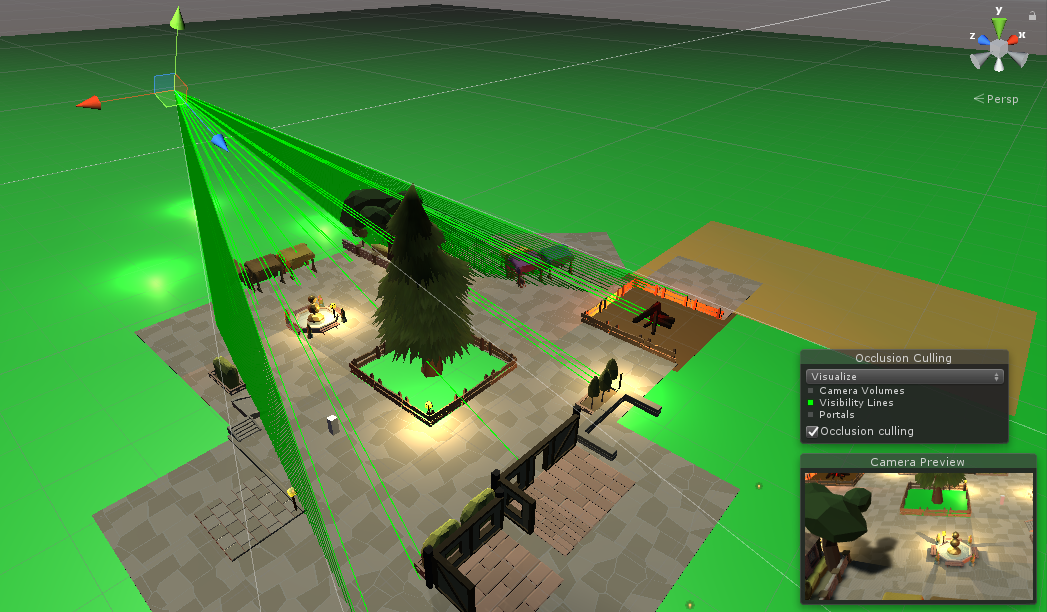
\includegraphics[scale=0.475]{images/village/occlusion_culling.PNG}
\caption{Occlusion Culling, Ignorieren von Objekten außerhalb des Sichtfeldes}
\label{fig:occlusion_culling}
\end{figure}

Unity stellt weiterhin eine Visualisierung für das Verfahren zur Verfügung. In der Abbildung \ref{fig:occlusion_culling} ist ein Beispiel für Occlusion Culling zu sehen. Das ausgewählte Objekt, das an den drei Achsen erkannt werden kann, ist die aktive Kamera der Szene. Ihre Position, Ausrichtung und die Breite ihres Sichtfelds bestimmen, welche Objekte berechnet werden müssen. In der rechten unteren Ecke der Abbildung ist der Ausschnitt der Szene zu erkennen, der von der Kamera wahrgenommen wird. In der Szene kann einfach erkannt werden, dass alle weiteren Objekte des Dorfes nicht angezeigt werden, weil sie vom Blickwinkel der Kamera nicht erfasst werden.
Die folgende Grafik \ref{fig:occlusion_culling_2} zeigt weiterhin, wie Objekte durch andere Objekte verdeckt werden. Hinter dem großen Gebäude im Vordergrund werden keine Objekte berechnet, das sie durch das Haus verdeckt werden. 

\begin{figure}[H]
\centering
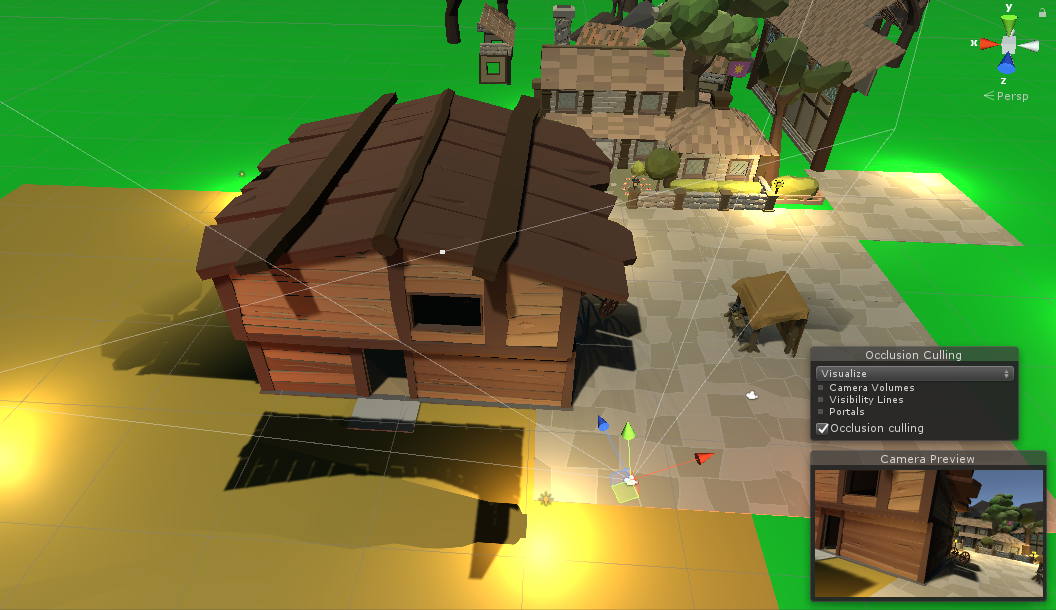
\includegraphics[scale=0.475]{images/village/occlusion_culling_2.PNG}
\caption{Occlusion Culling, Ignorieren von Objekten durch Verdeckung}
\label{fig:occlusion_culling_2}
\end{figure}



% anfangs wurden berufe nicht fest zugewiesen. bei der entscheidungsfindung konnten agenten aus allen work-aktionen auswählen, basierend auch auf der menge der resourcen. das hat dazu geführt, dass viele npcs das gleiche tun. daher wurden jobs fest zugewiesen. damit dann trotzdem die richtige menge von ressourcen produziert wurde, wurde der villageagent eingeführt. aber der funktioniert halt leider nicht.


\section{Verschiedene Ansätze für Ressourcensystem und VillageAgent}
Wie bereits in den Abschnitten \ref{village_village_agent} und \ref{gameacademy} beschrieben, sind durch die Parameter der \inlinecode{GameAcademy} verschiedene Ansätze für die Behandlung von Ressourcen und Berufen in der Simulation auswählbar. Insgesamt ergeben sich drei Möglichkeiten für die Verwaltung von Ressourcen:

\begin{itemize}
    \item \textit{Ansatz 1}: Keine Zuweisung von Berufen für Agenten. Es werden keine Berufsaktionen maskiert, stattdessen können Agenten die Aktionen frei wählen. Die Ressourcen werden durch die Auswahl der Aktionen der Agenten indirekt in der Balance gehalten.
    \item \textit{Ansatz 2}: Nutzung fest zugewiesener Berufe für Agenten sowie Maskierung aller Aktionen, die nicht zum Beruf gehören. Kontinuierliche Anpassung der Berufe durch den \inlinecode{VillageAgent} zur indirekten Verwaltung der Ressourcen.
    \item \textit{Ansatz 3}: Nutzung fest zugewiesener Berufe für Agenten ohne eine Anpassung durch den \inlinecode{VillageAgent}. Statt eine Lösung für das Ressourcenproblem zu finden, werden Ressourcen vollständig ignoriert und sind für die Entscheidungsfindung nicht mehr relevant.
\end{itemize}

Die Verwendung eines Ressourcensystems führt dazu, dass die Agenten lernen müssen, mit diesen Ressourcen umzugehen. Es besteht das Risiko, dass die Ressourcen des Dorfsystems ab einem gewissen Punkt nicht mehr in der Balance gehalten werden. Vor dem Training ist nicht absehbar, wie viele Ressourcen von den Agenten verbraucht werden, da nicht klar ist, welche Entscheidungen diese treffen. Es ist daher schwierig, für die Aktionen der Agenten sinnvolle Parameter bezüglich der Kosten und Erlöse von Ressourcen festzulegen. Daher werden Tests durchgeführt, die bestimmen sollen, mit welcher der drei oben genannten Verfahren das Problem am besten gelöst werden kann. Dazu gehört auch unter Umständen die Maßnahme, auf die Nutzung von Ressourcen gänzlich zu verzichten (Ansatz 3), falls kein zufriedenstellendes Ergebnis erzielt werden kann. 

Bevor weitere Aspekte des Trainings betrachtet werden, wird zunächst ein Vergleich zwischen drei Testtrainingsvorgängen der drei vorgeschlagenen Ansätze aufgestellt. In der Abbildung \ref{fig:diagram_test_resource_run_1} werden die Trainigsverläufe dargestellt.

\begin{figure}[H]
\centering
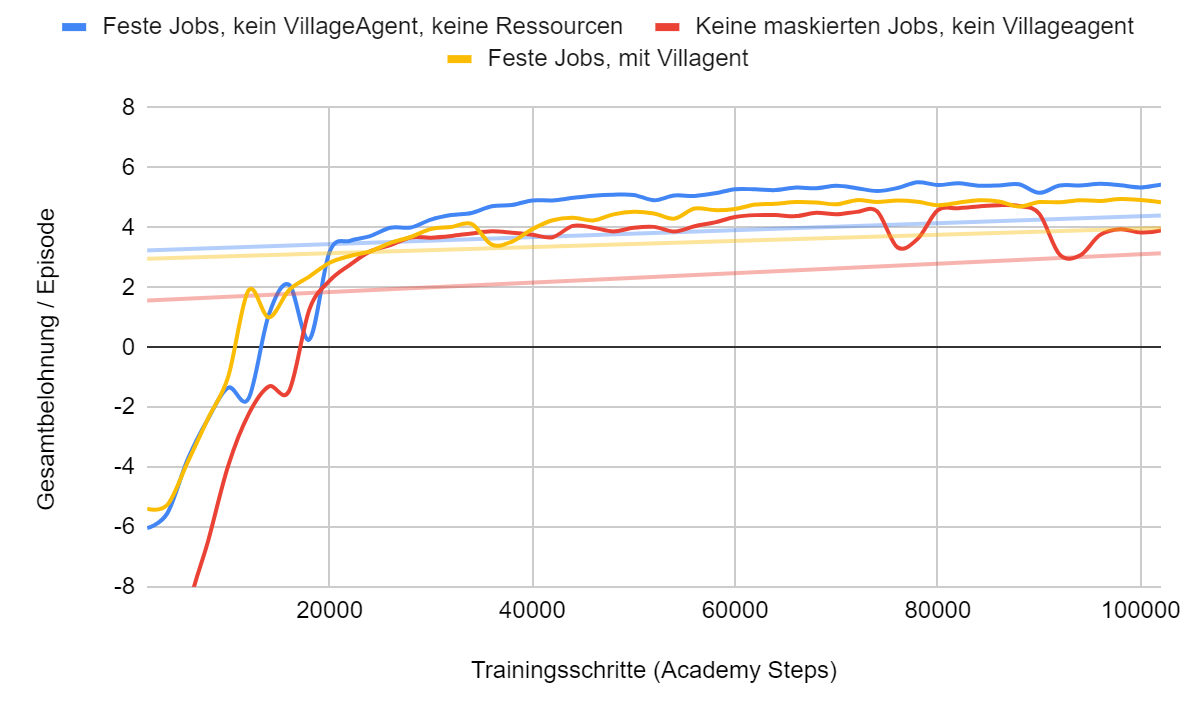
\includegraphics[scale=0.475]{images/training/diagram_test_resource_run_1.png}
\caption{Trainingsverläufe für \inlinecode{NpcAgent}s, verschiedene Ansätze für das Ressourcensystem}
\label{fig:diagram_test_resource_run_1}
\end{figure}

Grundsätzlich haben sich für alle Ansätze ähnliche Verläufe ergeben. Anhand der eingezeichneten Trendlinien kann man erkennen, dass sich für den ersten Ansatz insgesamt die niedrigsten akkumulierten Belohnungen ergeben haben. Das kann dadurch erklärt werden, dass ein insgesamt größerer Aktionsraum verwendet wurde. Dadurch wird das Training erschwert, weil dieser größere Aktionsraum erforscht werden muss, um Assoziationen zwischen Aktionen und Beobachtungen herzustellen. Für den zweiten Ansatz ergibt sich eine nur geringfügig niedrigere Belohnung im Vergleich zum ersten Ansatz. Aktionen werden im zweiten Ansatz öfter maskiert, weil Ressourcen nicht zur Verfügung stehen. Das kann dazu führen, dass Agenten gewünschte Aktionen nicht ausführen können, weil zu wenig Ressourcen vorhanden sind. Da diese Limitierungen für den dritten Ansatz nicht gelten und der Aktionsraum kleiner ist, wurden dort die höchsten Belohnungen erreicht. Nur im zweiten Ansatz wurde der \Fachbegriff{VillageAgent} verwendet. Neben den \inlinecode{NpcAgent}s mussten im entsprechenden Trainingsvorgang also auch \inlinecode{VillageAgent}s trainiert werden.
Insgesamt konvergieren alle drei Ansätze bereits nach etwa 400.000 Trainingsschritten. Die Graphen beschreiben anschließend einen nahezu flachen Verlauf. Ein signifikanter Lernvorgang ist nach dem Erreichen dieses Punktes nicht mehr zu erwarten.  

\begin{figure}[H]
\centering
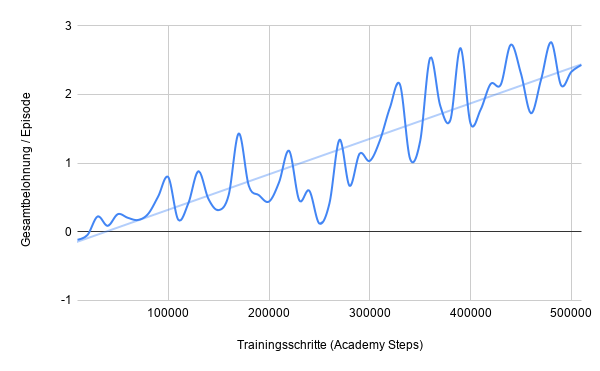
\includegraphics[scale=0.7]{images/training/diagram_test_resource_run_villageagent.png}
\caption{Trainingsverlauf des \inlinecode{VillageAgent}}
\label{fig:diagram_test_resource_run_villageagent}
\end{figure}

 In Abbildung \ref{fig:diagram_test_resource_run_villageagent} ist der Trainingsverlauf des \inlinecode{VillageAgent} zu erkennen. Der Verlauf der akkumulierten Belohnung steigt nicht monoton an. Es bildet sich ein eher unstabiles Training mit vielen lokalen Maxima und Minima ab. An der Trendlinie ist jedoch klar erkennbar, dass insgesamt ein Lernvorgang durch ein Wachstum der Belohnungen stattfindet. Weiterhin wird durch den Graphen bis zum Ende des Trainingsvorgangs kein Plateau abgebildet. Die akkumulierten Belohnungen verändern sich kontinuierlich. Aus diesem Grund wird ein erweiterter Trainingsprozess für den \inlinecode{VillageAgent} mit einer höheren Anzahl von Trainingsschritten durchgeführt, wie in Abbildung \ref{fig:diagram_test_resource_run_villageagent_LARGE} zu sehen.
 
\begin{figure}[H]
\centering
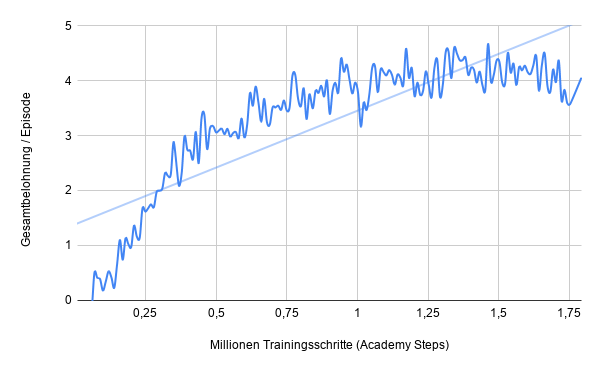
\includegraphics[scale=0.7]{images/training/diagram_test_resource_run_villageagent_LARGE.png}
\caption{Erweiterter Trainingsverlauf des \inlinecode{VillageAgent}}
\label{fig:diagram_test_resource_run_villageagent_LARGE}
\end{figure}

Auch im erweiterten Trainingsprozess ist zu erkennen, dass der entsprechende Graph nicht monoton steigt, sondern starke Schwankungen aufweist. Trotzdem ist wie bereits oben beschrieben ein konstantes Wachstum zu verzeichnen. Zum Ende des Verlaufs ist zu erkennen, dass der Graph einen flachen Verlauf beschreibt und das Wachstum der Belohnungen zum Stillstand kommt. Nach knapp mehr als einer Million Schritten wird annähernd ein Plateau erreicht.





% experimentiert mit resource rewards?


% rewards wurden erklärt, jetzt das wa seigentlich schief gelaufen ist (agenten sind dumm, oszillierender villageagent)







% beschreiben wie die trainingsverläufe aussehen


Die Betrachtung der akkumulierten Belohnungen alleine reicht allerdings noch nicht aus, um das Verhalten der Agenten zu beurteilen. Die aus den Trainingsvorgängen enstandenen Modelle bzw. Policies wurden daher im Inference-Modus der Simulation verwendet, um das Verhalten der Agenten zu betrachten und dadurch die Auswahl der verwendeten Ansätze zu beeinflussen. Es wurden jeweils mehrere Spielzeittage betrachtet, um das resultierende Verhalten der Agenten zu analysieren.

Im ersten Ansatz war auffällig, dass häufig viele Agenten den selben Beruf gewählt haben. Zeitweise haben etwa die Hälfte der 50 pro Dorf verwendeten Agenten dieselbe berufliche Tätigkeit ausgeführt. Die Agenten haben also nicht gelernt, Berufsaktionen aufgrund der aktuell vorhandenen Ressourcen zu wählen. Das führte dazu, dass das Ressourcensystem nicht in der Balance gehalten wurde und Defizite für bestimmte Ressourcen entstanden. Aus diesem Grund konnten nach einiger Zeit bestimmte Aktionen nicht mehr ausgeführt werden, weil ihre ressourcenbasierten Bedingungen nicht erfüllt wurden. Die trotzdem hohe Belohnung der Agenten ist darauf zurückzuführen, dass für maskierte Aktionen aufgrund von fehlenden Ressourcen in der Regel Alternativen verfügbar sind. Wenn zum Beispiel kein Bier mehr vorhanden ist, kann zwar die Freizeitaktion \Fachbegriff{Taverne} nicht mehr ausgeführt werden, wohl aber die Freizeitaktion \Fachbegriff{Visit}. Die Vielfältigkeit der Aktionen der Agenten wird dadurch jedoch eingeschränkt. Weiterhin bringt etwa das Ausführen der Berufsaktion \inlinecode{Logging} bei einem gegebenen Arbeitsbedürfnis die gleiche Belohnung wie die Aktion \inlinecode{Hunting}, sodass kein direkter Anreiz in Form von Belohnungen geboten wird, um unterschiedliche Berufsaktionen auszuführen. Die Verwendung der Ressourcen als Observations reicht daher nicht aus, um die Wahl der Beufsaktionen maßgeblich zu beeinflussen.
Verschiedene Ideen wurden verfolgt, um dieses Problem einzudämmen. Beispielsweise wurde für jede ausgeführte Aktion des Agenten eine zusätzliche Belohnung bzw. Bestrafung verteilt, die auf die Menge der Ressourcen zurückgeführt wurde - unabhängig davon, welche Aktion ausgeführt wurde. Außerdem wurde der Versuch unternommen, die Belohnungen beruflicher Aktionen an den produzierten Ressourcen im Vergleich zur aktuellen Menge der entsprechenden Ressource zu messen. Eine hohe Belohnung wurde dann erzielt, wenn ein Job ausgeführt wurde, dessen mit ihm verbundene Ressource nicht ausreichend vorhanden war.
Diese unternommenen Versuche konnten das Problem jedoch nicht beheben bzw. verschlechterten dieses teilweise. 

Daher wurde der im zweiten Ansatz verwendete \Fachbegriff{VillageAgent} entwickelt, der die Menge Ressourcen auf einem stabilen Level halten soll. Weiterhin wurden dafür die festen Berufe bzw. \Fachbegriff{Jobs} für Agenten eingeführt, die dazu führen, dass alle Aktionen eines Agenten, die nicht mit seinem Job assoziiert sind, maskiert werden. Für den Inference-Modus wurde der zweite, erweiterte Trainingsverlauf des \inlinecode{VillageAgent} verwendet (siehe Abbildung \ref{fig:diagram_test_resource_run_villageagent_LARGE}), um die bestmögliche Policy zu nutzen.
Wie bereits in Abschnitt \ref{village_village_agent} angedeutet, fällen alle verwendeten Agenten vom Typ \inlinecode{VillageAgent} immer dann eine Entscheidung, wenn ein Zähler in der \inlinecode{GameAcademy} einen bestimmten Wert erreicht. Die laufende Episode wird abgebrochen, sobald eine bestimmte Anzahl von Entscheidungen getroffen wurde. Der Zähler wird jedes mal inkrementiert, wenn ein \inlinecode{NpcAgent} eine Aktion ausführt. Die entsprechenden Parameter in der \inlinecode{GameAcademy} wurden so gewählt, dass alle \inlinecode{VillageAgent}s Entscheidungen ausführen, sobald jeder \inlinecode{NpcAgent} fünf Aktionen ausgeführt hat. Insgesamt sind zehn dieser Entscheidungen notwendig, um die Episode abzuschließen. Mit sechs verwendeten Dörfer und 50 pro Dorf verwendeten Agenten werden daher 1500 NPC-Aktionen gebraucht, um eine Entscheidung auszulösen und 15.000, um die Episode zu beenden.
Der \inlinecode{VillageAgent} erhält Belohnungen, wenn richtige Entscheidungen getroffen werden und Bestrafungen, wenn kontraproduktive Entscheidungen getroffen werden. Trotz eines kontinuierlichen Lernvorgangs und einer deutlich positiven akkumulierten Gesamtbelohnung kommt es nicht dazu, dass das Ressourcensystem durch eine Anpassung der Berufe in Waage gehalten wird. Das System oszilliert stark und lernt nicht ausreichend, Entscheidungen zu treffen, die auf der aktuellen Menge der Ressourcen beruhen. Ein grundlegendes Problem bei diesem Vorgang ist die Häufigkeit der Entscheidungen, die durch den Agenten gefällt werden - auf 1000 gesammelte Erfahrungen durch \inlinecode{NpcAgent}s kommen lediglich ca. 4 Erfahrungen des \inlinecode{VillageAgent}s. Der \inlinecode{VillageAgent} muss also aus einer Menge von Entscheidungen eine Policy erlernen, die nur einem Anteil von 0.4\% der entsprechenden Menge des \inlinecode{NpcAgent} entspricht. Um den Zustandsraum des Agenten hinreichend zu erkunden, muss vermutlich eine deutlich höhere Anzahl von Erfahrungen gesammelt werden. Ein zusätzliches potentielles Problem besteht darin, dass die Auswirkungen der Entscheidungen auf die tatsächlichen Ressourcenmengen eine starke zeitliche Verzögerung haben, da Agenten nur etwa ein mal am Tag arbeiten. Das kann theoretisch dazu führen, dass die gleichen Aktionen mehrfach ausgeführt werden, weil die Menge der Ressourcen sich seit der letzten Entscheidung nicht signifikant verändert hat. Es wurden Versuche unternommen, diese Probleme zu lösen, indem die Belohnungen und die Intervalle der \inlinecode{VillageAgent}-Entscheidungen angepasst wurden. Diese Versuche führten ebenfalls dazu, dass den NPCs falsche Berufe zugewiesen wurden.

Aus diesem Grund wird der dritte Ansatz verwendet, in dem das Ressourcensystem ignoriert wird. Aktionen produzieren und verbrauchen dann keinerlei Ressourcen mehr. Weiterhin werden keine ressourcenbasierte Observations getätigt und keine Belohnungen an Ressourcen gebunden.

Dadurch wird der Simulation ein kleiner Teil ihrer Komplexität genommen. Die Glaubwürdigkeit der Entscheidungsfindung der NPCs wird dadurch allerdings nicht beeinflusst, da diese maßgeblich von den Bedürfnissen des Agenten abhängt. Die Nutzung von Ressourcen fungiert viel mehr als limitierender Faktor. Um die Agenten tatsächlich authentischer wirken zu lassen, müsste das Ressourcensystem um Faktoren wie Handel zwischen verschiedenen Dörfern erweitert werden. Da dies nicht gegeben ist, stellt das Ignorieren des Ressourcensystems keine Verschlechterung dar.    




\section{Wahl der initialen Hyperparameter}\label{village_training_hyperparameter}
Die Tabelle \ref{tab:ml-agents_training_hyperparameters} zeigt eine Übersicht über die wichtigsten Hyperparameter für das Training der Agenten. Diese werden in einer Konfigurationsdatei definiert, wie in Abschnitt  \ref{ml_unity} beschrieben. Für die Erstellung der Übersicht dient eine Tabelle aus der ML-Agents Dokumentation als Grundlage \cite{ml-agents_documentation_hyperparameter_ppo}, die Empfehlungen für die Parameter ausspricht. Alle nicht \ac{ppo}-basierten Parameter wurden aus der Tabelle entfernt, da sie für diese Arbeit nicht weiter relevant sind.

\smallskip
\begin{table}[H]
\begin{tabular} {|  p{3.2cm}  |  p{12.4cm}  |} \hline
\textbf{Setting} & \textbf{Description} \\ \hline
batch\_size & The number of experiences in each iteration of gradient descent. \\ \hline
beta & The strength of entropy regularization. \\ \hline
buffer\_size & The number of experiences to collect before updating the policy model. \\ \hline
epsilon & Influences how rapidly the policy can evolve during training. \\ \hline
hidden\_units & The number of units in the hidden layers of the neural network. \\ \hline
lambd & The regularization parameter. \\ \hline
learning\_rate & The initial learning rate for gradient descent. \\ \hline
max\_steps & The maximum number of simulation steps to run during a training session. \\ \hline
memory\_size & The size of the memory an agent while training with a recurrent network. \\ \hline
normalize & Whether to automatically normalize observations. \\ \hline
num\_epoch & The number of passes to make through the experience buffer when performing gradient descent optimization. \\ \hline
num\_layers & The number of hidden layers in the neural network. \\ \hline
behavioral\_cloning & Use demonstrations to bootstrap the policy neural network. \\ \hline
reward\_signals & The reward signals used to train the policy. Curiosity and GAIL can be enabled here. Gamma can also be set here. \\ \hline
sequence\_length & Defines how long the sequences of experiences must be while training. Only used for training with a recurrent neural network. \\ \hline
summary\_freq & How often, in steps, to save training statistics. This determines the number of data points shown by TensorBoard. \\ \hline
time\_horizon & The amount of experiences collected per-agent before adding it to the experience buffer. \\ \hline
use\_recurrent & Train using a recurrent neural network. \\ \hline
\end{tabular}
\caption{ML-Agents-Hyperparameter für das Training \cite{ml-agents_documentation}}
\label{tab:ml-agents_training_hyperparameters}
\end{table}

Ein Großteil dieser Parameter wurde bereits durch mathematische Grundlagen im Kapitel \ref{reinforcement_learning}  definiert. Die Funktion weiterer Parameter geht entweder aus der Beschreibung innerhalb der Tabelle hervor oder wird in der folgenden Tabelle \ref{village_training_hyperparameter} erläutert. Einige der Parameter sind optional.


Für das Training der Agenten wurden mehrere Trainingsvorgänge mit unterschiedlichen Hyperparametern durchgeführt, die später miteinander verglichen werden. Als Grundlage für das Training wird der im vorherigen Abschnitt beschriebene Trainingsvorgang für den dritten Ansatz der Lösung für den Umgang mit Ressourcen verwendet. Die in diesem Vorgang verwendete Trainingskonfiguration, die im Folgenden vorgestellt wird, stellt eine Basiskonfiguration dar, die das Fundament für weitere Trainingsvorgänge bildet. In diesen Vorgängen werden jeweils einzelne Parameter aus der Konfiguration angepasst. Dadurch sollen möglichst ideale Hyperparameter identifiziert werden. Bereits die in der Basiskonfiguration festgelegten Parameter wurden empirisch ermittelt, indem während der Entwicklung des Dorfes zahlreiche Trainingsvorgänge durchgeführt wurden.
Schließlich wird ein finales Training durchgeführt, das die besten verwendeten Hyperparameter nutzt und so ein optimales Ergebnis erzielen soll. Im Folgenden werden Hyperparameter für den zugrunde liegenden Trainingsvorgang beschrieben. Für die initiale Festlegung der Trainingsparameter wurden teilweise Empfehlungen aus der Dokumentation des ML-Agents Frameworks hinzugezogen \cite{ml-agents_documentation_hyperparameter_ppo}. Ein Großteil der Parameter wurde bereits im Kapitel \ref{reinforcement_learning} erläutert und ist auf die mathematischen Grundlagen des Verfahrens zurückzuführen. Folgende Parameter wurden für das Basistraining verwendet:

\smallskip
\begin{table}[H]
\footnotesize
\centering
\begin{tabular} {|  p{3.5cm}  |  p{3cm}  |} \hline
\textbf{Parameter} & \textbf{Beschreibung} \\ \hline

\Fachbegriff{trainer}  &  ppo  \\ \hline
\Fachbegriff{epsilon}  &  0.2  \\ \hline
\Fachbegriff{lambd}  &  0.925  \\ \hline
\Fachbegriff{learning\_rate\_schedule}  &  linear  \\ \hline
\Fachbegriff{learning\_rate}  &  4e-4  \\ \hline
\Fachbegriff{max\_steps}  &  5e5  \\ \hline
\Fachbegriff{normalize}  &  false  \\ \hline
\Fachbegriff{batch\_size}  &  32  \\ \hline
\Fachbegriff{buffer\_size}  &  8192  \\ \hline
\Fachbegriff{num\_epoch}  &  4  \\ \hline
\Fachbegriff{time\_horizon}  &  512  \\ \hline
\Fachbegriff{beta}  &  1.2e-2  \\ \hline
\Fachbegriff{summary\_freq}  &  2000  \\ \hline
\Fachbegriff{num\_layers}  &  3  \\ \hline
\Fachbegriff{hidden\_units}  &  256  \\ \hline
\Fachbegriff{use\_recurrent}  &  false  \\ \hline
\Fachbegriff{memory\_size}  &  128  \\ \hline
\Fachbegriff{sequence\_length}  &  128  \\ \hline
\Fachbegriff{reward\_signals}  &  extrinsic  \\ \hline
\Fachbegriff{reward\_strength}  &  1.0  \\ \hline
\Fachbegriff{gamma}  &  0.93  \\ \hline

\end{tabular}
\caption{Gewählte Hyperparameter für das Basistraining.}
\label{tab:base_training_hyperparameters}
\end{table}

Als zugrunde liegender Algorithmus wird \ac{ppo} verwendet. \Fachbegriff{epsilon} wird auf $ 0.2 $ festgelegt. Der Wert bestimmt, wie groß Änderungen der Policy minimal sein müssen. Über den Parameter \Fachbegriff{lambd} kann definiert werden, wie sehr sich der Algorithmus auf die Vorhersage (bzw. \Fachbegriff{Value Estimate}) der Belohnung im Gegensatz zur eigentlichen erfahrenen Belohnung einer Aktion verlässt. Es wird eine Lernrate mit dem Wert $4 * 10^{-4}$ verwendet, die sich im Verlauf des Trainingsvorgangs linear bis zum Wert $0$ beim letzten Trainingsschritt verringert. Insgesamt werden dafür 500.000 Trainingsschritte verwendet. Eine Normalisierung der Observations findet nicht statt, da alle Beobachtungen manuell normalisiert werden.
Weiterhin muss ein Wert für die \Fachbegriff{buffer\_size} festgelegt werden. Dadurch wird beschrieben, wie viele Entscheidungen gesammelt werden sollen, bevor ein Update der Policy stattfindet. Dieser Buffer wird in Batches von der Größe \Fachbegriff{batch\_size} aufgeteilt. Für jeden dieser Batches wird ein Gradientenverfahren durchgeführt, um das neue, angepasste Modell zu berechnen. Der Parameter \Fachbegriff{num\_epoch} legt fest, wie oft dieser Prozess wiederholt werden soll. Der Parameter \Fachbegriff{time\_horizon} legt fest, wie viele Entscheidungen auf einmal in den Buffer geschrieben werden sollen. Wenn die Kapazität des Buffers vor dem Beenden einer Episode erreicht wurde, wird ein \Fachbegriff{Value Estimate} gebildet, um die zukünftigen Belohnungen des Agenten der Episode zu schätzen. \Fachbegriff{buffer\_size} und \Fachbegriff{time\_horizon} müssen daher logischerweise ein Vielfaches der \Fachbegriff{batch\_size} sein. Diese Parameter wurden durch Empfehlungen des Frameworks und empirische Beobachtungen ausgewählt. Konkret wurden noch während der Entwicklung der Dorfsimulation verschiedene Trainingsvorgänge ausgeführt, wobei sich bestimmte Parameter bewährt haben.

Über den Wert \Fachbegriff{beta} wird definiert, wie zufällig die Aktionen der Agenten ausgewählt werden, um zu gewährleisten, dass der Aktionsraum des Agenten sinnvoll erkundet wird. Damit wird also direkt die Entropie beeinflusst, die festlegt, wie zufällig die Entscheidungen eines Brains sind. Der Wert sollte so ausgewählt werden, dass die Entropie des Trainingsvorgangs stetig sinkt.

Über die \Fachbegriff{summary\_freq} kann die Schrittgröße für die Ausgabe der durchschnittlichen akkumulierten Belohnung der Agenten in der Konsole bestimmt werden. Größere Werte führen zu einem zu hohen Intervall zwischen Statusberichten. Zu kleine Werte führen zu einer starken Varianz bezüglich der erfahrenen Belohnungswerte. In diesem Fall wird für jeweils 2.000 durchgeführte Trainingsschritte ein Statusbericht angegeben. 

Die Parameter \Fachbegriff{num\_layers} und \Fachbegriff{hidden\_units} sind essentiell für den Aufbau des neuronalen Netzes. Insgesamt werden drei Schichten mit je 512 enthaltenen Neuronen verwendet. Es wird kein rekurrentes neuronales Netz verwendet, da der Parameter \Fachbegriff{use\_recurrent} auf \Fachbegriff{false} gesetzt wird. Die \Fachbegriff{memory\_size} bestimmt die Größe für einzelne \sogenannt{Erinnerungen} für die Rückkopplungen in dem rekurrenten Netz. Über den Parameter \Fachbegriff{sequence\_length} wird zudem festgelegt, wie viele dieser Erinnerungen verwendet werden sollen. Diese Parameter werden nur für rekurrente neuronale Netze verwendet und sind daher zunächst nicht relevant.

Der Wert des \Fachbegriff{reward\_signals} bestimmt, welche Art von Belohnungen das Verfahren verwendet und wird daher auf \Fachbegriff{extrinsic} festgelegt. Damit sind die Belohnungen gemeint, die in der Simulation festgelegt wurden. Es können zusätzliche \Fachbegriff{reward\_signals} festgelegt werden, um mehrere Belohnungsarten zu nutzen. Durch \Fachbegriff{curiosity}-Belohnungen erhält der Agent immer dann Belohnungen, wenn er von seiner Policy abweicht, um den Aktionsraum zu erkunden. Das ist dann sinnvoll, wenn extrinsische Belohnungen sehr selten sind und nur durch \sogenannt{Ausprobieren} gefunden werden können. Da in diesem Fall jede Aktion eine Belohnung zur Folge hat, werden zunächst keine derartigen Belohnungen verwendet. Zusätzlich können \Fachbegriff{GAIL}-Belohnungen verwendet werden, die nicht relevant sind, da sie bei Imitation Learning zum Einsatz kommen.
Konkret werden extrinsische Belohnungen mit einem Multiplikator \Fachbegriff{reward\_strength} von $1.0$ verwendet, da die in der Simulation definierten Belohnungen nicht verändert werden sollen. Weiterhin wird ein relativ niedriger Wert \Fachbegriff{gamma} festgelegt. Dieser Parameter beschreibt den in Kapitel \ref{reinforcement_learning} definierten Wert $ \gamma $ und bestimmt, wie sehr zukünftige Belohnungen Entscheidungen des Agenten beeinflussen. 
Für $ \gamma\ $ wird ein niedriger Wert gewählt, sodass zukünftige Zustände des Agenten weniger relevant sind. Es wird davon ausgegangen, dass für die Befriedigung von menschlichen Bedürfnissen hauptsächlich der aktuelle Zustand relevant ist. 



\section{Güteüberprüfung}
Beim überwachten Lernen werden häufig direkte Bewertungskriterien genutzt, indem Werte für \Fachbegriff{Precision}, \Fachbegriff{Recall} oder \Fachbegriff{F1} gebildet werden. Da beim \ac{reinforcement_learning} keine Klassifizerung stattfindet und keine gelabelten Daten vorhanden sind, ist ein derartiges Vorgehen hier nicht möglich. Ein exakter Wert für die Genauigkeit der Ergebnisse kann daher nicht gebildet werden.
Um die Güte der Trainingsergebnisse zu überprüfen, können alternative Metriken verwendet werden. Neben der Höhe der Belohnungen wird die \Fachbegriff{Value Loss}-Funktion verwendet. Sie beschreibt die Verlustfunktion (siehe Abschnitt \ref{loss_functions}) bezüglich der Value Function des Agenten und gibt damit an, wie gut das Modell Belohnungen zukünftiger Zustände vorhersagen kann. Weiterhin wird der  Entropieverlauf genutzt, der die Zufälligkeit der gewählten Aktionen bestimmt. Die Daten können im Tensorboard betrachtet und von dort exportiert werden. Im Normalfall kann man auch an der Länge der Episoden den Lernvorgang bewerten. Die Länge der Episoden der Agenten ist hier aber nicht relevant, da die Episoden stets nach einer festgelegten Anzahl von Aktionen enden.

Mit den genannten Metriken kann zwar der Erfolg des Trainingsvorgang aus einer mathematischen Sicht evaluiert werden, sie bieten jedoch nur Hinweise darüber, wie authentisch das resultierende Verhalten der Agenten ist. Um das tatsächliche Verhalten zu bewerten, reichen diese Metriken also nicht aus. Hohe Belohnungen könnten zum Beispiel auch entstehen, wenn ein Agent lernt, einen Fehler in der Simulation auszunutzen. Daher müssen die Agenten konkret innerhalb der Simulation im Inference-Modus beobachtet werden. Dafür können die entwickelten UI-Elemente, die Auskunft über verschiedene Informationen des Dorfes wie der Anzahl der aktuell ausgeführten Aktionen bieten, genutzt werden. Diese Informationen bieten einen schnellen Überblick über das erlernte Verhalten der Agenten. Im Abschnitt \ref{7_result_agent_behavior} wird neben Metriken wie der Entropie oder den Belohnungen der Agenten daher zusätzlich das Verhalten der Agenten betrachtet.













\section{Trainingsergebnisse}
Wie im vorherigen Abschnitt erwähnt, wurde eine Basiskonfiguration für Trainingsvorgänge erstellt, auf deren Grundlage Trainingsvorgänge durchgeführt werden. Einzelne Parameter werden für diese Vorgänge angepasst, anschließend wird ein Vergleich der Ergebnisse durchgeführt.

Zunächst wird der Basistrainingsvorgang näher betrachtet.

\subsection{Basistraining}
In den Abbildungen \ref{fig:diagram_test_resource_run_entropy}, \ref{fig:base_value-loss} und \ref{fig:base_reward} sind Informationen zum Basistrainingsverlauf zu erkennen. Auf den horizontalen Achsen der Diagramme ist jeweils die Anzahl der Trainingsschritte eingezeichnet.

\begin{figure}[H]
\centering
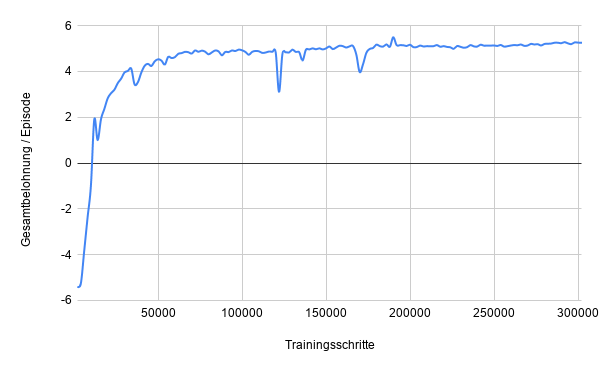
\includegraphics[scale=0.7]{images/training/base_reward.png}
\caption{Akkumulierte Belohnungen im Basistraining des \inlinecode{NpcAgent}}
\label{fig:base_reward}
\end{figure}

\begin{figure}[H]
\centering
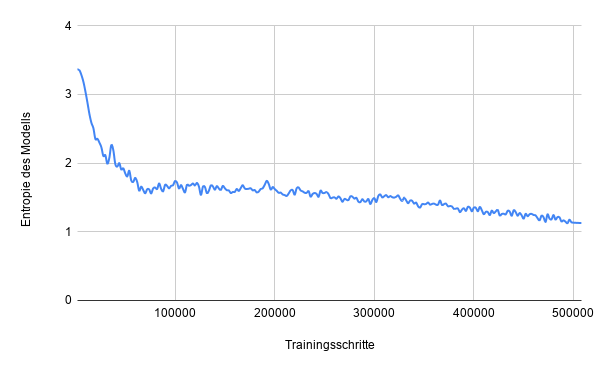
\includegraphics[scale=0.7]{images/training/base_value-loss.png}
\caption{Value Loss im Basistraining des \inlinecode{NpcAgent}}
\label{fig:base_value-loss}
\end{figure}

Die Abbildung \ref{fig:base_value-loss} zeigt den Verlauf des \Fachbegriff{Value Loss}, also die Verlustfunktion bezüglich der Value Function. Solange der Graph einen absteigenden Verlauf beschreibt, lernt der Agent, die Value Function zu optimieren.

\begin{figure}[H]
\centering
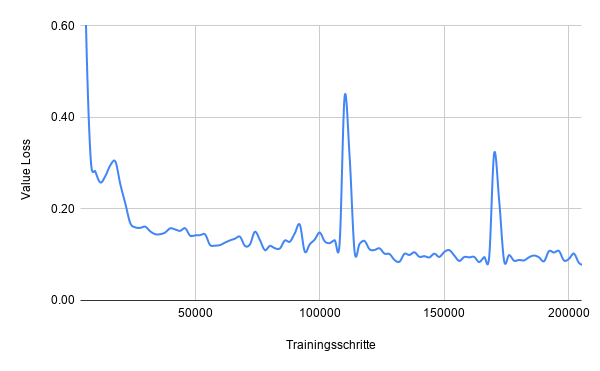
\includegraphics[scale=0.7]{images/training/base_entropy.png}
\caption{Entropieverlauf im Basistraining des \inlinecode{NpcAgent}}
\label{fig:diagram_test_resource_run_entropy}
\end{figure}

Die Entropie wurde auf den Wert $ 1.2 * 10^{-2}$ festgelegt. Daraus ergibt sich der in Abbildung \ref{fig:diagram_test_resource_run_entropy} sichtbare Entropieverlauf. Die stetige Verringerung der Entropie mit einer steigenden Anzahl der Trainingsschritte belegt, dass ein guter Wert gewählt wurde.

Weiterhin beschreibt die Abbildung \ref{fig:base_reward} die akkumulierten Belohnungen für das Basistraining, wie bereits in Teilen in Abbildung \ref{fig:diagram_test_resource_run_1} zu sehen. Man kann erkennen, dass sich die Spitzen der Belohnungsfunktion bei etwa  125.000 und 170.000 Zeitschritten im Value Loss-Diagramm widerspiegeln. Typischerweise sinkt die Verlustfunktion so lange, wie die Belohnung des Agenten zunimmt. Weiterhin sind keine Auffälligkeiten zu erkennen.










\subsection{Optimierung der Ergebnisse durch Anpassung der Hyperparameter}
Um optimale Parameter zu definieren, wurde eine Reihe von Trainingsvorgängen durchgeführt. In jedem dieser Durchläufe wurde ein einzelner Parameter aus der Basiskonfiguration angepasst, um die Auswirkungen der Änderung isoliert zu betrachten. Das Ergebnis wird mit anderen Trainingsvorgängen verglichen, in dem der selbe Parameter verändert wurde. Es wird geprüft, ob die Veränderung eine Verbesserung erzielt. Der Parameter mit dem besten Trainingsresultat wird anschließend für ein finales Training gewählt und in die finale Konfigurationsdatei eingetragen. Über mehrere Tage wurden dafür Trainingsdurchläufe durchgeführt. 
Die jeweilige Dauer der durchgeführten Trainingsvorgänge kann in der Abbildung \ref{fig:training_durations} betrachtet werden. Auffällig ist, dass das Training mit einem rekurrenten Netzwerk deutlich mehr Zeit beansprucht, da durch die zusätzlichen Verbindungen der Neuronen im Netzwerk ein höherer Rechenaufwand entsteht. Darüber hinaus sind keine Besonderheiten zu verzeichnen. Alle Trainingsvorgänge haben in etwa die selbe Zeit in Anspruch genommen. Für weitere leichte Schwankungen wird eine variable Auslastung der CPU verantwortlich gemacht, da die verwendete Hardware zur Trainingszeit teilweise mit weiteren Aufgaben gefordert wurde.

\begin{figure}[H]
\centering
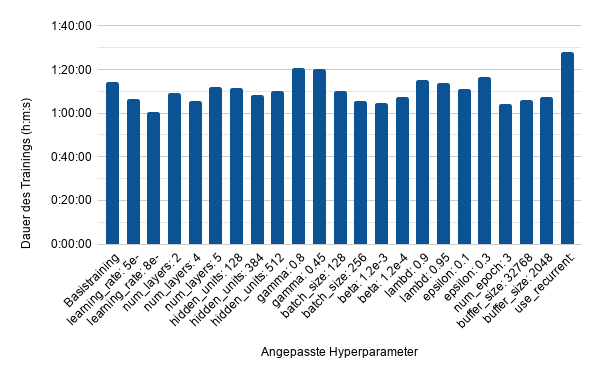
\includegraphics[scale=0.65]{images/training/training_durations.png}
\caption{Dauern der unterschiedlichen Trainingsvorgänge}
\label{fig:training_durations}
\end{figure}

Nach dem Vergleich der Ergebnisse sollte ein verlängertes, finales Training durchgeführt werden. Es wurde davon ausgegangen, dass die Parameter unabhängig voneinander verändert und schließlich kombiniert werden können, um ein optimales Ergebnis zu erzielen. Es hat sich allerdings gezeigt, dass die Nutzung mehrerer Parameteränderungen, die jeweils ein besseres Ergebnis im Vergleich zum Basistraining erzielt haben, in Kombination nicht zwangsweise ein besseres Ergebnis zur Folge haben. Damit wurde gezeigt, dass es starke Abhängigkeiten zwischen den einzelnen Parametern gibt.
In der Abbildung \ref{fig:final_training_failure} ist die entstandene Belohnungsfunktion aus diesem Training zu sehen. Es ist leicht zu erkennen, dass die Gesamtbelohnungen mit einem Maximalwert von ca. $2.6$ deutlich unter dem Niveau des Basistrainings liegen.

\begin{figure}[H]
\centering
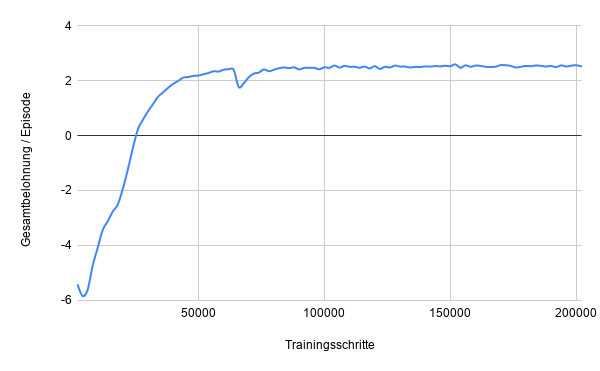
\includegraphics[scale=0.65]{images/training/final_training_failure.png}
\caption{Belohnungsfunktion durch Kombination der optimalen Einzelparameter}
\label{fig:final_training_failure}
\end{figure}

Die Ergebnisse der ausgeführten Einzeltrainings geben trotzdessen eine Auskunft über die Anpassung der Parameter im Einzelnen. Sie sind im Anhang A zu finden und werden durch Diagramme dokumentiert.

Um bei vorhandenen Abhängigkeiten zwischen den Parametern die optimalen Werte zu finden, hätte nach der Ermittlung eines neues, besseren Parameters bereits die Basiskonfiguration mit diesem Parameter angepasst werden müssen, sodass die Anpassung bei weiteren Trainingsvorgängen bereits miteinbezogen wurde.

Insgesamt stellt die Wahl der Hyperparameter ein schwieriges Problem dar, da extrem viele Kombinationen verschiedener Werte für Hyperparameter durchgeführt werden können. Einige Werkzeuge und Frameworks für Machine Learning bieten eine automatisierte Auswahl für Hyperparameter an, indem eine Menge von Kombinationen verschiedener Kandidaten für Parameter geprüft werden, um das beste Ergebnis zu erlangen. Ein Beispiel für dieses Vorgehen ist die sogenannte \Fachbegriff{Exhaustive Grid Search} \cite{scikit_gridsearch} des Frameworks \Fachbegriff{scikit-learn} \cite{scikit-learn}. Im Falle von ML-Agents gibt es so eine automatisierte Suche der Parameter nicht. Die Dauer der nötigen Trainingsvorgänge würde weiterhin deutlich zu hohe Maßstäbe annehmen.


\subsection{Finaler Trainingsvorgang}
Im vorherigen Abschnitt wurde der Versuch unternommen, optimale Trainingsparameter zu ermittelt, in dem eine Reihe von Testtrainingsdurchläufen ausgeführt wurde. Anschließend wurde ein verlängertes Trainingsvorgang mit diesen Parametern durchgeführt, wodurch schlechte Werte für die Belohnungen der Agenten erreicht wurden.   

Da nicht das gewünschte Ergebnis erzielt wurde, wurden weitere Testtrainingsvorgänge durchgeführt. Es wurde festgestellt, dass bei einer Verringerung der Lernrate auf $1e-4$ und einer Erhöhung der Batchgröße auf $64$ bessere Ergebnisse erzielt werden können. Zusätzlich wird die Anzahl der Trainingsschritte auf \Fachbegriff{1e6} erhöht. Mit diesen Parametern wird nun ein finales, verlängertes Training durchgeführt, das zu einem verbesserten Lernvorgang führen soll. In den folgenden Diagrammen sind die Resultate dieses Trainingsvorgangs abgebildet.

Im Vergleich zum Basistraining wurden unmittelbar leicht verbesserte Ergebnisse für alle drei verwendeten Metriken erzeugt. Durch die Verlängerung des Trainings konnte weiterhin ein leichter, stetiger Anstieg bei der Belohnungsfunktion und ein leichter, stetiger Abstieg für die Entropie und den Value Loss ausgenutzt werden, um insgesamt bessere Ergebnisse zu erlangen.
Die maximale Belohnung beträgt im Basistraining 5,241 und im finalen Training 5,429. Die Gesamtbelohnung pro Episode wurde damit um ca. 3,6\% gesteigert. Der minimale Value Loss wurde von 0,073 auf 0,037 verbessert. Weiterhin konnte die Entropie von 1,127 auf 0,642 verringert werden.

\begin{figure}[H]
\centering
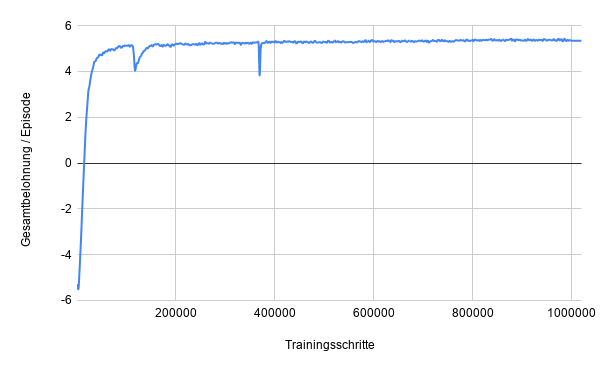
\includegraphics[scale=0.7]{images/training/final/final_rewards.png}
\caption{Akkumulierte Belohnungen im finalen Training des \inlinecode{NpcAgent}}
\label{fig:final_rewards}
\end{figure}

\begin{figure}[H]
\centering
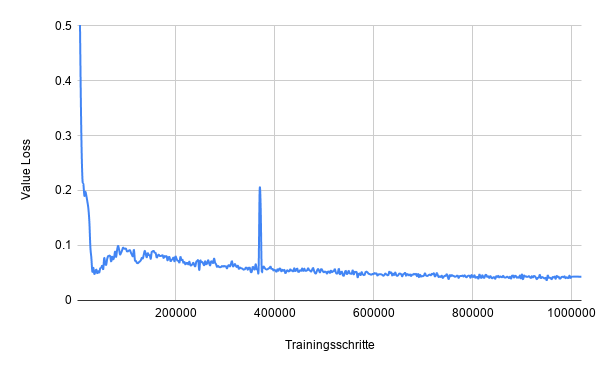
\includegraphics[scale=0.7]{images/training/final/final_loss.png}
\caption{Value Loss im finalen Training des \inlinecode{NpcAgent}}
\label{fig:final_loss-loss}
\end{figure}

\begin{figure}[H]
\centering
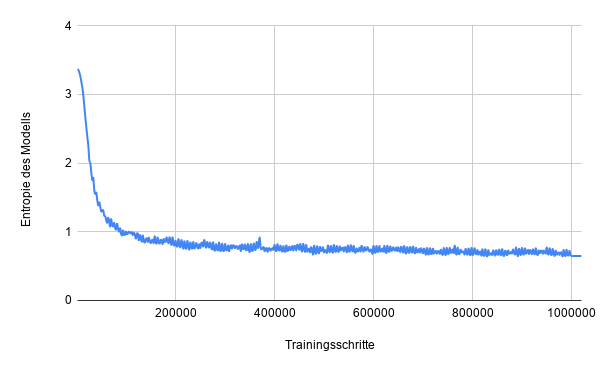
\includegraphics[scale=0.7]{images/training/final/final_entropy.png}
\caption{Entropieverlauf im finalen Training des \inlinecode{NpcAgent}}
\label{fig:final_entropy}
\end{figure}








\subsection{Verhalten der Agenten}\label{7_result_agent_behavior}
Durch den finalen Trainingsvorgang wurde ein Modell für die Entscheidungsfindung der NPCs erzeugt. Das Modell bestimmt das Verhalten der Agenten, das im Folgenden untersucht wird.


\subsubsection{Eindruck}
Der erste Eindruck erweckt den Anschein einer belebten Stadt, in der viele NPCs unterschiedliche Tätigkeiten ausführen. Es wirkt lebendig, da in allen Bereichen des Dorfes NPCs umherlaufen. Damit wird zunächst genau der Eindruck erzielt, der vermittelt werden soll. Dem Anschein nach befindet sich der Spieler in einer belebten Welt, in der eine Vielzahl von Agenten ihrem persönlichen Leben nachgehen. Durch die Betrachtung der Informationen im UI ist weiterhin auffällig, dass unterschiedliche Aktionen ausgeführt werden.


\subsubsection{Auswahl von Aktionen aufgrund von Bedürfnissen}
Über einen längeren Zeitraum wurden mehrere Agenten näher betrachtet. Dabei wurde für jede Aktion, die sie ausgeführt haben, auf ihre Bedürfnisse geachtet, um zu bewerten, ob die Entscheidungen der Agenten sinnvoll sind. Dabei wurde festgestellt, dass die Agenten in fast allen Fällen eine Entscheidung treffen, die für einen Beobachter unter Berücksichtigung der Bedürfnisse des Agenten sinnvoll erscheinen. Aus diesen Beobachtungen kann gefolgert werden, dass die Agenten erfolgreich gelernt, haben, aufgrund ihrer Bedürfnisse Entscheidungen zu treffen, die diese befriedigen. In dem überwiegenden Großteil der Beobachtungen wählten die Agenten Aktionen für das Bedürfnis, das den niedrigsten Bedürfniswert hatte.
Im \inlinecode{NeedCycleHandler} wurden für die Bedürfnisse \Fachbegriff{Hunger}, \Fachbegriff{Durst}, \Fachbegriff{Bildung}, \Fachbegriff{Kommunikation} und \Fachbegriff{Glauben} Konstanten festgelegt. Diese bestimmen den Zyklus der Bedürfnisse und damit die Steigung der Bedürfnisfunktion und die Dauer bis zum Erreichen eines kritischen Bedürfnislevels. In den Beobachtungen aus der Dorfsimulation spiegelt sich die unterschiedliche Dauer der Zyklen wider. Die verschiedenen Bedürfnisse werden in unterschiedlichen zeitlichen Abständen befriedigt. Die definierten Konstanten decken sich dabei mit dem Ausführungsrhytmus der jeweiligen Aktionen. Das Glaubensbedürfnis erreicht zum Beispiel nach drei Tagen den Wert $0$. Etwa alle drei Tage wird das Bedürfnis gestillt.

Im Gegensatz zu den genannten Basisbedürfnissen kann weiterhin festgestellt werden, dass die NPCs in regelmäßigen Abständen arbeiten und schlafen. Das ist sinnvoll, weil das Schlaf- und das Arbeitsbedürfnis direkt von der simulierten Zeit des Dorfes abhängt. Dadurch entsteht für die Agenten ein grober Tagesablauf. Zusätzlich wurde die Beobachtung aufgestellt, dass die Agenten relativ genau ein mal pro Tag schlafen und arbeiten.



\subsubsection{Beitrag der Attribute zur Entscheidungsfindung}
Während der Entwicklung der Simulation kam es häufig dazu, dass Agenten bestimmte Aktionen bevorzugt haben, da für diese die höchste Belohnung erwartet wurde. Das ist besonders für \Fachbegriff{Recreation}-Aktionen relevant, da diese Aktionen alle dasselbe Bedürfnis befriedigen. Um das Problem zu umgehen, wurden die Belohnungen der Aktionen von den Attributen der Agenten abhängig gemacht. Weiterhin ist der Beruf des Agenten ausschlaggebend für die Attribute der Agenten. In der folgenden Abbildung ist die resultierende Verteilung der Attribute in Abhängigkeit von den Berufen zu sehen:

\begin{figure}[H]
\centering
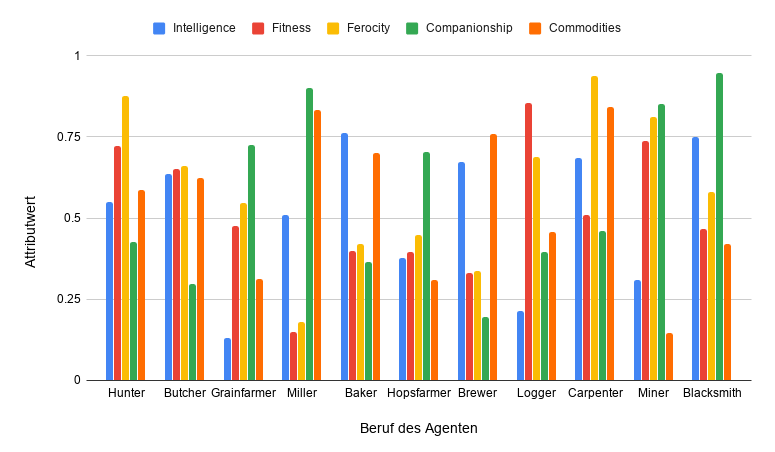
\includegraphics[scale=0.6]{images/training/attribute_job_results.png}
\caption{Verteilung der Attribute und Berufe der Agenten}
\label{fig:attribute_job_results}
\end{figure}

Weiterhin wird in der folgenden Grafik \ref{fig:attribute_action_results} die durchschnittlichen Höhe der Attribute von Agenten für Recreation-Aktionen dargestellt. In einer Tabelle werden zusätzlich die jeweiligen Attribute festgehalten, die für die Belohnungen der Recreation-Aktionen genutzt werden. Dafür werden die Identifier für die Aktionen und Attribute genutzt. Die Belohnungen für Attribute können invertiert werden, sodass ein hohes Attribut für die Aktion zu einer Strafe führt. 

\begin{figure}[H]
\centering
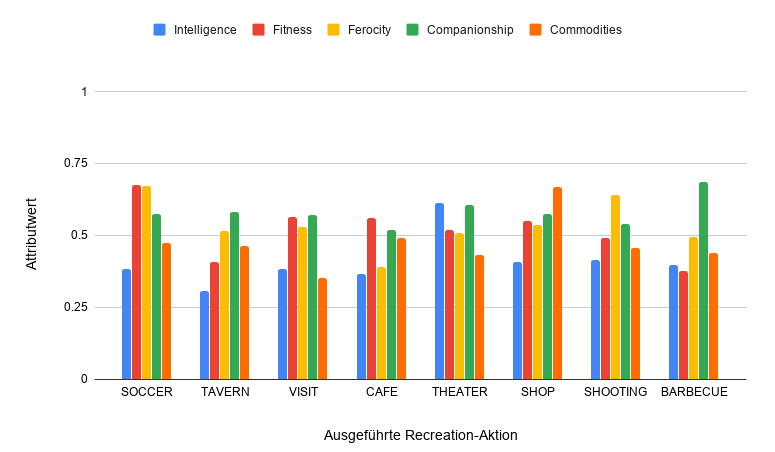
\includegraphics[scale=0.6]{images/training/attribute_action_results.png}
\caption{Verteilung der Attribute und Berufe der Agenten}
\label{fig:attribute_action_results}
\end{figure}

\smallskip
\begin{table}[H]
\begin{tabular} {|  p{5cm}  |  p{10.6cm}  |} \hline
\textbf{Aktion} & \textbf{Attribute} \\ \hline
RECREATION\_SOCCER & ATT\_FITNESS, ATT\_FEROCITY. \\ \hline
RECREATION\_TAVERN & ATT\_INTELLIGENCE (invertiert), ATT\_FITNESS (invertiert). \\ \hline
RECREATION\_VISIT & ATT\_COMPANIONSHIP, ATT\_COMMODITIES (invertiert). \\ \hline
RECREATION\_THEATER & ATT\_INTELLIGENCE. \\ \hline
RECREATION\_CAFE & ATT\_COMPANIONSHIP, ATT\_FEROCITY (invertiert). \\ \hline
RECREATION\_SHOP & ATT\_COMMODITIES, ATT\_FEROCITY (invertiert). \\ \hline
RECREATION\_SHOOTING & ATT\_FEROCITY, ATT\_COMPANIONSHIP (invertiert). \\ \hline
RECREATION\_BARBECUE & ATT\_COMPANIONSHIP, ATT\_FITNESS (invertiert). \\ \hline

\end{tabular}
\caption{Beeinflussing der Belohnungen von Recreation-Aktionen durch Attribute}
\label{tab:recreation_actions_attributes}
\end{table}

Die Verteilung der Attribute deckt sich ungefähr mit den Attributboni, die in der obigen Tabelle dargestellt werden. Dadurch wird gezeigt, dass die Attribute der Agenten bei der Wahl der Recreation-Aktion eine Rolle spielen. Agenten mit Attributen, die einen Bonus für die Belohnung einer bestimmten Aktion zur Folge haben, führen diese Aktion also statistisch gesehen häufiger aus als andere Aktionen. Die im Abschnitt \ref{agents_rewards} angesprochene Einteilung der Agenten in Gruppen wurde daher erreicht. Auch durch simple Beobachtungen lässt sich diese Eigenschaft überprüfen; beispielsweise trifft man in der Taverne tatsächlich häufiger Agenten mit einem niedrigen Intelligenzlevel an, wie etwa Bauern oder Holzarbeiter.




\subsubsection{Tagesablauf und Bedürfnisverlauf}
Die durchschnittlichen Bedürfnisse der Agenten wurden über einen Zeitraum von 100 Simulationstagen beobachtet und zu bestimmten Tageszeiten festgehalten. Schließlich wurden von allen Agenten die mittleren Bedürfniswerte für bestimmte Tageszeiten berechnet, wie in Abschnitt \ref{village_logging} beschrieben. Daraus hat sich der folgende Bedürfnisverlauf ergeben:

\begin{figure}[H]
\centering
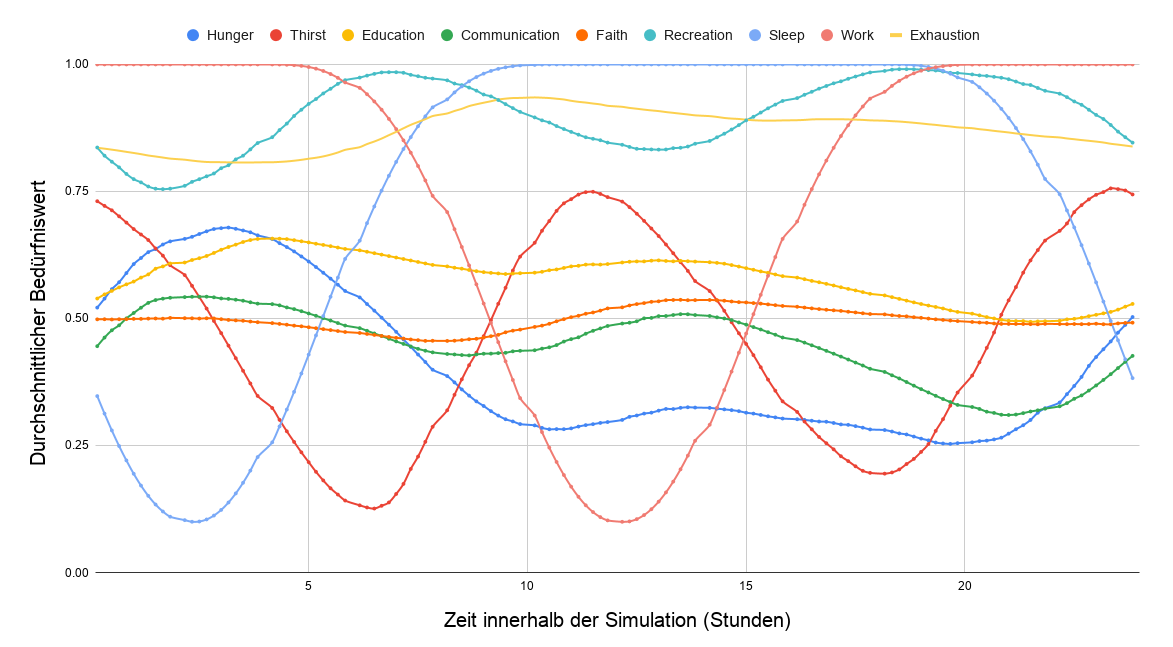
\includegraphics[scale=0.4]{images/training/reinforcement_needs_day_cycle.png}
\caption{\ac{reinforcement_learning}-Ansatz, Verlauf der durchschnittlichen Bedürfniswerte}
\label{fig:reinforcement_needs_day_cycle}
\end{figure}

Zum Verlauf der Bedürfnisse wird angemerkt, dass die Variable \inlinecode{\_rythmVariation} zur Erzeugung eines Offsetes zwischen Agenten im \inlinecode{NeedCycleHandler} (siehe Abschnitt \ref{npc_needs_architecture}) für die Aufzeichnung der Daten deaktiviert wurde. Dadurch sollen Unterschiede zwischen den Agenten eliminiert werden. Der gezeigte Verlauf ist zwar repräsentativ für alle Agenten, normalerweise würde für jeden einzelnen Agenten jedoch eine horizontale Verschiebung der Bedürfnisse durch die Verwendung des Offsets entstehen.
Weiterhin entsprechen die gewählten Schlaf- und Arbeitszeiten nicht unbedingt dem durchschnittlichen Menschen unserer heutigen Gesellschaft, da bei der Entwicklunge der Zyklen mit normalisierten Float-Werten zwischen 0 und 1 gearbeitet wurde. Die Schlaffunktion erreicht ihr Minimum erst um etwa 2:30 Uhr nachts. Für das Verhalten des Agenten spielt dies jedoch keine Rolle. Durch eine simple Transformation könnten die Zyklen verschoben werden, in dieser Analyse werden sie jedoch in der vorliegenden Form akzeptiert.

Weiterhin kann man feststellen, dass sich die Bedürfnisse nicht zufällig entwickeln, sondern von der jeweiligen Tageszeit abhängen. Es sind Kurven entstanden, die Hinweise darauf geben, wann Bedürfnisse befriedigt werden.

Die Hungerfunktion wurde so gewählt, dass sie nach einem halben Tag den Wert $0$ erreicht. Am Verlauf des Hungers ist zu erkennen, dass das Bedürfnis in der Nacht zunächst zunimmt und dann sinkt, sobald sich die Agenten schlafen legen. Das Hungergefühl wächst dann automatisch an, weil der Agent mit der Aktion \Fachbegriff{Schlafen} beschäftigt ist. Über den Tag verteilt bleibt das Hungergefühl auf einem relativ gleichbleibenden aber akzeptablen Level. Das spricht dafür, dass die Agenten zu unterschiedlichen Zeiten essen. Ob der Agent direkt nach dem Aufwachen essen muss, hängt von den zuvor getätigten Aktionen und somit den aktuellen Bedürfnissen des Agenten ab.
Das Durstgefühl des Agenten wird hingegen von einer deutlich stärker schwankenden Funktion beschrieben, die einer Sinuskurve ähnelt. Die Durstfunktion wurde so definiert, dass sie etwa drei mal am Tag den Wert $0$ erreicht, wenn das Durstgefühl nicht gestillt wird. Tatsächlich ist an dem Graphen zu erkennen, dass die Agenten zwei mal am Tag ihr Durstgefühl stillen - nach dem Aufwachen und nach der Arbeit. Schlussfolgernd muss sich das Durstgefühl des Agenten für eine gewisse Zeit auf dem Wert $0$ befinden. Das bedeutet nicht, dass der Agent die falschen Aktionen getroffen hat - zur gleichen Zeit können mehrere Bedürfnisse den Wert $0$ annehmen. Die Belohnungen für die Bedürfnisse \Fachbegriff{Arbeit} und \Fachbegriff{Schlaf} sind darüber hinaus deutlich höher als die Belohnungen für weitere Bedürfnisse. Das bedeutet, dass ein Agent, der hungrig und durstig ist, sich trotzdem für die Aktion \Fachbegriff{Arbeit} entscheiden würde, wenn das entsprechende Bedürfnis klein genug ist. Die Belohnungen wurden so gewählt, um einen gleichbleibenden Tagesablauf des Agenten zu gewährleisten. Weiterhin haben alle Aktionen eine gewisse Dauer. Erst nachdem die Dauer der Aktion vorüber ist, kann eine weitere Aktion ausgeführt werden, die ein zwischenzeitlich auf den Wert $0$ gesunkenes Bedürfnis befriedigen soll. Solange die erste Aktion und selbst die zweite Aktion noch ausgeführt wird, kann dieses Bedürfnis auf dem Wert $0$ stagnieren. Erst nachdem die zweite Aktion beendet wurde, wird das Bedürfnis aufgefüllt.
Es ist daher logisch, dass der Agent nur zwei mal am Tag seinen Durst stillt, obwohl das Bedürfnis theoretisch drei mal am Tag auf den Wert $0$ sinkt, denn die Ausführung der \Fachbegriff{richtigen} Aktion ist nicht immer möglich, etwa, weil der Agent mit anderen Dingen beschäftigt ist.

Die Bedürfnisse nach Bildung und Glauben bleiben über den gesamten Tag auf einem relativen ähnlichen Level. Das liegt daran, dass erst nach 1,9 Tagen das Bildungs- und erst nach drei Tagen das Glaubensbedürfnis auf den Wert $0$ abgefallen ist. Da Exponentialfunktionen für die Berechnung der Bedürfnisse verwendet wurden, sind die beiden Bedürfnisse für den Großteil dieser Zeit auf einem hohen Level in der Nähe des Wertes $1$. Beide Bedürfnisse verzeichnen einen leichten Anstieg um etwa 10:00 Uhr, was darauf hindeutet, dass Agenten um diese Zeit häufig ihr Glaubens- und Bildungsbedürfnis befriedigen. Weiterhin hat das Bildungsbedürfnis einen leichten Anstieg um etwa 22:00 Uhr.

Das Bedürfnis nach Kommunikation verhält sich auf ähnlich wie das Bedürfnis nach Bildung. Dieses Bedürfnis sinkt nach 0,95 Tagen auf den Wert $0$ ab. Besonders häufig wird es um etwa 20:30 befriedigt, nachdem der Agent von der Arbeit gekommen ist und etwas getrunken hat. Analog zu diesem Verlauf sind etwa um diese Zeit in der Simulation viele Dorfbewohner auf dem Marktplatz zu sehen, die sich treffen, um zu kommunizieren.
Die \Fachbegriff{Exhaustion} sinkt über den Tag langsam ab. Sobald die Agenten schlafen, erhöht sich das Bedürfnis automatisch wieder, da die Agenten sich erholen. Es sind keine starken Steigungen zu beobachten, die darauf hinweisen, dass sich Agenten zu bestimmten Zeiten ausruhen.

Sowohl das Schlaf- als auch das Arbeitsbedürfnis werden nicht durch die Aktionen der Agenten beeinflusst. Stattdessen hängen sie direkt von der Zeit in der Simulation ab. Sie erfüllen lediglich den Zweck, die Belohnungen der Agenten von einer Bedürfnisfunktion abhängig zu machen, die Bedürfnisse lassen sich aber nicht auffüllen. Sobald ein Agent schläft oder arbeitet, dauern die entsprechenden Aktionen so lange, dass bei der Beendigung wieder der Wert $1$ für das Bedürfnis erreicht wird. Die in der Abbildung \ref{fig:village_diagram_sleep_work_functions} dargestellten Funktionen sind in der oben zu sehenden Grafik gut wiederzuerkennen. Die Zeitpunkte der Befriedigung der weiteren Bedürfnisse hängt vom Schlaf- und Arbeitsbedürfnis indirekt ab. Durch die Etablierung dieser beiden zeitabhängigen Bedürfnisse wurde das Fundament für den weiteren Tagesablauf der Agenten gelegt. Sie bestimmen, wann der Agent Zeit für weitere Aktionen hat. Durch die hohe Dauer der Aktionen verringern sich weiterhin automatisch stark die Bedürfnisse des Agenten, sobald er arbeitet oder schläft. Es ist daher logisch und notwendig, dass ein NPC direkt nach dem Arbeiten oder Schlafen etwas trinken muss.





\subsubsection{Dauer der Aktionen}
Über einen Zeitraum von 100 Simulationstagen wurde die Dauer aller Aktionen gespeichert. Schließlich wurde aus der Menge der Dauer für eine Aktion der jeweilige Durchschnitt berechnet, wie in Abbildung \ref{fig:avereage_action_durations} zu sehen.

\begin{figure}[H]
\centering
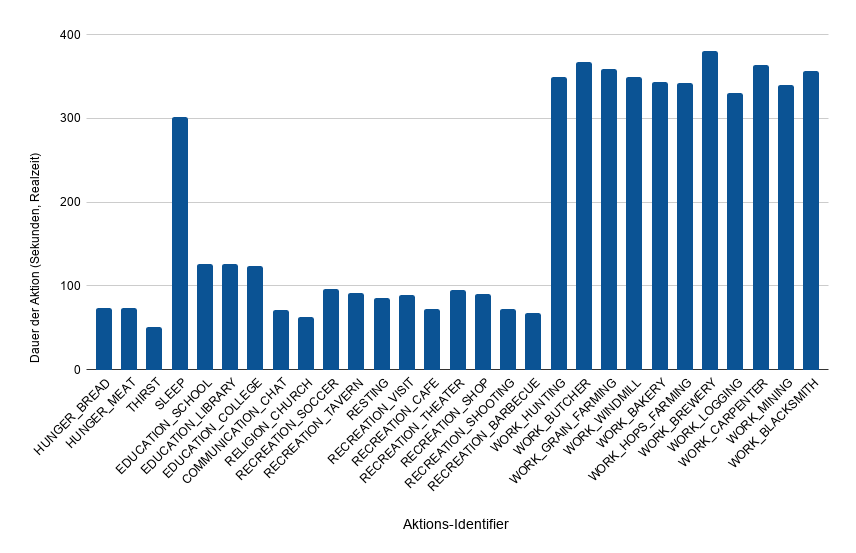
\includegraphics[scale=0.5]{images/training/avereage_action_durations.png}
\caption{Durchschnittliche Dauer der Aktionen}
\label{fig:avereage_action_durations}
\end{figure}

Die Teilaktionen der ActionPlans wurden so festgelegt, dass Aktionen, die dasselbe Bedürfnis befriedigen, möglichst gleich viel Zeit benötigen. Die Abbildung zeigt, dass die Ausführung der Recreation-Aktionen ähnlich viel Zeit braucht. Weiterhin stimmen die Dauern der beruflichen Aktionen ungefähr überein. Die in den Teilaktionen festgelegten Dauern wurden daher korrekt gewählt.

Die Festlegung der Dauern ist besonders schwierig, weil sich der Startort eines Agenten bei der Ausführung einer Aktion stets ändert. Daher variiert die benötigte Dauer, um zum Zielort zu gelangen. Die Abbildung zeigt, dass die Teilaktionen der ActionPlans gut definiert wurden, da insgesamt die gewünschten Dauern erreicht wurden.  


\subsubsection{Anzahl der Aktionen im Verhältnis}
Um einen Eindruck über die relativen Häufigkeiten der Aktionen zu erlangen, wurden über einen Zeitraum von 100 Simulationstagen die Mengen der jeweils ausgeführten Aktionen gespeichert. Dieses Verhältnis wird in der folgenden Abbildung dargestellt:
 
\begin{figure}[H]
\centering
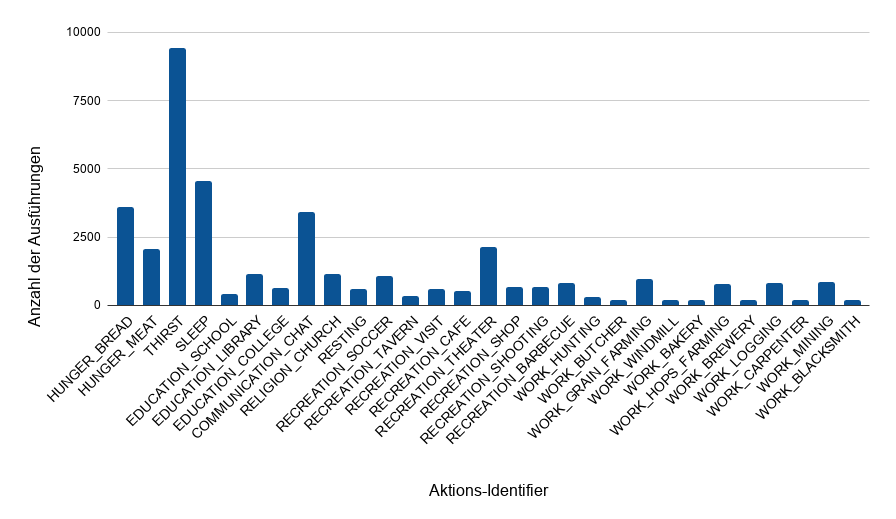
\includegraphics[scale=0.5]{images/training/actions_amounts_relation.png}
\caption{Verhältnis der Menge der ausgeführten Aktionen}
\label{fig:actions_amounts_relation}
\end{figure}

Insgesamt wurden 38.799 Aktionen von 50 Agenten ausgeführt. Im Durchschnitt hat jeder Agent also ca. 804 Aktionen insgesamt bzw. ca. 7,76 Aktionen pro Tag ausgeführt. Die jeweilige Anzahl der entsprechenden Aktionen deckt sich mit den im \inlinecode{NeedCycleHandler} festgelegten Zyklusdauern sowie den in der Abbildung \ref{fig:reinforcement_needs_day_cycle} beobachteten Verläufen. Das Bedürfnis \Fachbegriff{THIRST} wird zum Beispiel deutlich häufiger befriedigt als das Bedürfnis \Fachbegriff{FAITH}, da unterschiedliche Zyklusdauern festgelegt wurden.

Die Aktion \inlinecode{EDUCATION\_LIBRARY} wurde deutlich häufiger als andere Bildungs-Aktionen ausgeführt. Das liegt daran, dass die Altersgruppe für die Bibliothek deutlich mehr Agenten beinhaltet als die des College oder der Schule.

Auffällig ist lediglich, dass unproportional viele Agenten die Aktion \inlinecode{RECREATION\_THEATER} ausgeführt haben. Diese Anomalie könnte zum einen damit erklärt werden, dass ein Fehler im Programmcode vorliegt, oder zum anderen, dass der Trainingsvorgang nicht ideal verlaufen ist. 


\subsubsection{Maskierte Aktionen}
Weiterhin wurde die Anzahl der maskierten Aktionen untersucht. Für die Entscheidungen aller Agenten wurde dafür die Menge der maskierten Aktionen gespeichert. Da NPCS feste Berufe haben und deswegen nur eine berufliche Aktion ausführen können, beträgt die Menge der maskierten Berufsaktionen - mit Ausnahme der Aktion, die zum Job des Agenten gehört - genau der Menge der insgesamt ausgeführten Aktionen. Ähnlich verhält es sich mit den Bildungs-Aktionen, da diese vom Alter des Agenten abhängen. Alle anderen Aktionen wurden im Durchschnitt lediglich zwei Mal maskiert, was bei über 800 ausgeführten Aktionen für das Training nicht nennenswert ins Gewicht fallen sollte.
\chapter{Weitere entwickelte Ansätze}\label{weitere_ansaetze}
Um einen Vergleich des entwickelten Ansatzes zu weiteren Technologien aufstellen zu können, wurden zwei weitere Verfahren für die Implementierung der Entscheidungsfindung intelligenter Agenten verwendet. 
Die grundsätzliche Struktur der Dorfsimulation bleibt dabei erhalten. Die Entscheidungsfindung der Agenten dagegen ändert sich maßgeblich.
Es wurde ein regelbasierter sowie ein \ac{goap}-basierter Ansatz entwickelt. Im Folgenden werden diese vorgestellt.


\section{Regelbasierter Ansatz}
Für den regelbasierten Ansatz wurde die Klasse \inlinecode{ManualDecisionMaker} erstellt. Der Aufbau der Klasse ist in Abbildung \ref{fig:architecture_diagram_manualdecisionmaker} zu erkennen:

\begin{figure}[H]
\centering
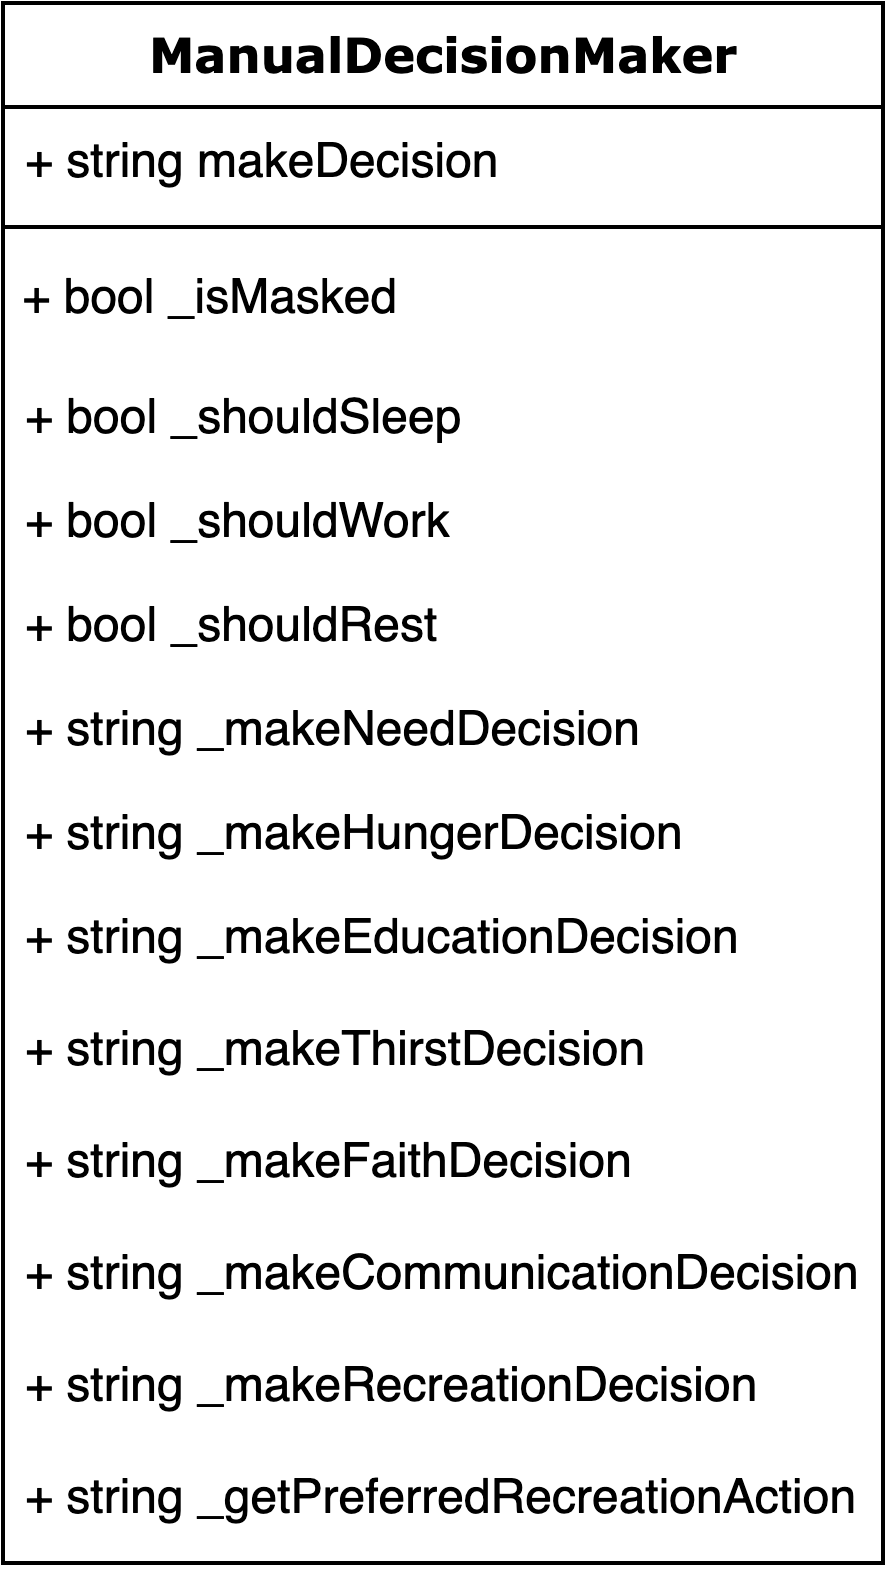
\includegraphics[scale=0.20]{images/village/architecture_diagram_manualdecisionmaker.png}
\caption{Methoden der Klasse \inlinecode{Manual Decision Maker}}
\label{fig:architecture_diagram_manualdecisionmaker}
\end{figure}

Der \inlinecode{ManualDecisionMaker} übernimmt die Entscheidungsfindung, indem er den Zustand des Agenten betrachtet und auf der Grundlage von bestimmten Regeln die beste Aktion auswählt. Die Klasse ersetzt im Architekturdiagram (siehe Abbildung \ref{fig:architecture_general}) die Rolle des externen Tensorflow-Backends welches für die Entscheidungsfindung zuständig ist. Die Klasse \inlinecode{NpcAgent} wird also weiterhin verwendet, alle Funktionen des ML-Agents-Frameworks werden aber deaktiviert. Da der \inlinecode{NpcAgent} bereits über alle nötigen Abhängigkeiten, Handler und Komponenten verfügt, wird der generelle Aufbau der Architektur nicht weiter verändert. Die Methode \inlinecode{requestModelOrManualDecision} ruft dann statt der ML-Agents-Funktion \inlinecode{RequestDecision} die Funktion \inlinecode{makeDecision} in der Klasse \inlinecode{ManualDecisionMaker} auf, um abhängig vom Zustand des Agenten Entscheidungen zu treffen. Die Funktion \inlinecode{makeDecision} ist im folgenden Listing \ref{lst:manual_decision_maker_make_decision} zu sehen:

\begin{minipage}{\linewidth}
\begin{lstlisting}[linewidth=16.4cm, label=lst:manual_decision_maker_make_decision, caption=Funktion \inlinecode{makeDecision} im \inlinecode{ManualDecisionMaker}, xleftmargin=1cm, basicstyle=\footnotesize]
public string makeDecision() {
    _mask = _npc.ActionMaskingHandler.getStringActionMask(_npc);

    if (_shouldSleep()) return NpcActions.SLEEP;
    if (_shouldWork()) return _npc.NpcState.AgentInfo.JobId;
    if (_shouldRest()) return NpcActions.RESTING;

    string action = _makeRecreationDecision();
    if (action != null) return action;

    action = _makeNeedDecision();
    if (action != null) return action;

    Debug.LogWarning("Could not find a good action for the agent. Choosing a random action that is not masked instead.");
    List<string> unmaskedActions = new List<string>();
    foreach (string actionId in NpcActions.ALL_ACTIONS) {
        if (!_mask.Contains(actionId)) unmaskedActions.Add(actionId);
    }
    if (unmaskedActions.Count != 0) {
        return unmaskedActions[Mathf.RoundToInt(Random.value * (unmaskedActions.Count - 1))];
    }
    Debug.LogWarning("Could not manage to find ANY actions for the agent! Choosing an action that IS MASKED instead.");
    return NpcActions.ALL_ACTIONS[Mathf.RoundToInt(Random.value * (NpcActions.ALL_ACTIONS.Length - 1))];
}
\end{lstlisting}
\end{minipage}

Eine Reihe von Bedingungen werden der Reihe nach mit absteigender Priorität abgearbeitet. Unter anderem wird dabei die Ausführbarkeit der Aktion geprüft, indem ermittelt wird, ob diese durch \inlinecode{\_mask} maskiert ist. Sobald eine Bedingung zutrifft, gibt die jeweils aufgerufene Funktion den Identifier einer Aktion in Form eines Strings zurück. Wenn der Rückgabewert \Fachbegriff{null} ist, wird die nächste Bedingung bearbeitet. Zunächst wird geprüft, ob der Agent schlafen, arbeiten oder ruhen muss.
Wenn keine dieser Bedingungen zutrifft, wird mittels \inlinecode{\_makeRecreationDecision} ermittelt, ob ein niedriger Wert für die Recreation des Agenten vorliegt, sodass dieser eine Freizeitaktivität ausführen sollte. Es werden ebenfalls die Attribute des Agenten mit einbezogen. Eine Liste aus allen Attributen des Agenten wird absteigend sortiert. Mit der Funktion \inlinecode{getPreferredAttributeAction} aus der Klasse \inlinecode{AttributeHandler} wird nun für jedes Attribut in der Liste nacheinander geprüft, ob die durch die Attribute des Agenten präferierte Aktion ausführbar ist.

Falls keine Recreation-Aktion gefunden wurde, werden schließlich die Bedürfnisse des Agenten betrachtet. Die entsprechende Funktion ist in Listing \ref{lst:manual_decision_maker_need_decision} zu finden. Ähnlich wie bei den Attributen wird eine Liste von allen Bedürfnissen sortiert, hier jedoch aufsteigend. Der Reihe nach wird dann in einem \Fachbegriff{switch-case} geprüft, ob die mit dem Bedürfniss verbundenen Aktionen ausführbar sind.

\begin{minipage}{\linewidth}
\begin{lstlisting}[linewidth=16.4cm, label=lst:manual_decision_maker_need_decision, caption=Funktion \inlinecode{makeNeedDecision} im \inlinecode{ManualDecisionMaker}, xleftmargin=1cm, basicstyle=\footnotesize]
private string _makeNeedDecision() {
    List<KeyValuePair<string, float>> needs = new List<KeyValuePair<string, float>>();
    foreach (string needType in NpcState.ALL_NEEDS) {
        needs.Add(new KeyValuePair<string, float>(needType, _npcState.getNeedByType(needType)));
    }
    needs.Sort((x, y) => x.Value.CompareTo(y.Value));

    foreach (KeyValuePair<string, float> need in needs) {
        string decision = null;
        switch (need.Key) {
            case NpcState.NEED_HUNGER:
                decision = _makeHungerDecision();
                break;
            case NpcState.NEED_THIRST:
                decision = _makeThirstDecision();
                break;
            case NpcState.NEED_EDUCATION:
                decision = _makeEducationDecision();
                break;
            case NpcState.NEED_COMMUNICATION:
                decision = _makeCommunicationDecision();
                break;
            case NpcState.NEED_FAITH:
                decision = _makeFaithDecision();
                break;
        }
        if (decision == null) continue;
        else return decision;
    }
    return null;
}
\end{lstlisting}
\end{minipage}

Wenn auch bei diesem Vorgehen keine gültige Aktion gefunden wird, wird eine zufällige Aktion gewählt, die nicht maskiert ist. Wenn auch das scheitert, wird eine zufällige maskierte Aktion ausgewählt. Alternativ könnte der Agent ebenfalls so lange keine Aktion ausführen, bis eine Aktion verfügbar ist.







\section{Goal Oriented Action Planning}
Weiterhin wurde ein Ansatz entwickelt, der auf \ac{goap} basiert (siehe Kapitel \ref{goap}). Nicht alle Features des Dorfes, die im Kapitel \ref{entwicklung_dorf} vorgestellt wurden, sind in diesem Verfahren funktionsfähig. Es handelt sich eher um ein Proof-Of-Concept, das das generelle Vorgehen der Implementierung von \ac{goap} dokumentieren soll.

Im Folgenden wird die Architektur des Ansatzes beschrieben. Zunächst wird auf die wichtigsten Komponenten der verwendeten Bibliothek eingegangen.


\subsection{Verwendete GOAP-Bibliothek}
Für die Implementierung wurde die Open Source-Bibliothek \Fachbegriff{GOAP} genutzt \cite{goap_library}. Zunächst werden die wichtigsten Klassen der Bibliothek beschrieben.

\subsubsection{GoapAction}
Die Klasse \inlinecode{GoapAction} beschreibt eine ausführbare GOAP-Aktion, die bestimmte Bedingungen erfordert und Effekte verursacht. Sie dient als Grundlage für die Erzeugung des Aktionsbaumes, der den Weg von einem Startpunkt über Aktionen zu einem Ziel bzw. Goal beschreibt.

Im Konstruktor der Klasse werden Effekte hinzugefügt. Diese werden in der Klasse \inlinecode{Effects} definiert und im Feld \inlinecode{List<string> effects} gespeichert. Äquivalent dazu werden in der Variablen \inlinecode{preconditions} Bedingungen festgehalten. Weiterhin muss eine Reichweite \inlinecode{requiredRange} festgelegt werden. Später wird dieser Wert für die Navigation des Agenten zum Zielort benutzt. In dem Feld \inlinecode{cost} werden darüber hinaus die Kosten für die Aktion festgelegt.
Schließlich muss die Funktion \inlinecode{Perform} überschrieben werden, um die eigentlich Aktion auszuführen - beispielsweise das Warten eines Agenten für einen bestimmten Zeitraum an einem bestimmten Ort.

\subsubsection{GoapGoal}
Um das Ziel eines Agenten zu beschreiben, wird in der Klasse \inlinecode{Goal} ein Identifier für ein neues Goal anhand einer String-Konstante erzeugt. Dieses Ziel wird einer bestimmten Aktion zugewiesen, deren Ausführung das Erreichen des Ziels beschreiben soll. Die Zuweisung erfolgt in dem Feld \inlinecode{goal} der \inlinecode{GoapAction}.
Weiterhin muss eine neue Klasse erstellt werden, die von der Klasse \inlinecode{GoapGoal} erbt und direkt mit dem definierten Ziel verbunden ist. Die entsprechende String-Konstante, die das Ziel beschreibt, ist ein Parameter für den Konstruktor des \inlinecode{GoapGoal}. Nun wird eine Liste aller Aktionen erstellt, die das entsprechende Ziel haben.

\subsubsection{GoapAgent}
Die Klasse \inlinecode{GoapAgent} verwaltet alle Aktionen und Goals des Agenten. Der Aktionsbaum für die Entscheidungsfindung des Agenten wird hier aufgebaut.
Zunächst werden alle verfügbaren Aktionen mithilfe der Funktion \inlinecode{AddAction} hinzugefügt. Ebenfalls werden alle erzeugten Goals in das Feld \inlinecode{Dictionary<string, GoapGoal>} mit aufgenommen.
Für jedes der Goals wird nun anhand der Effekte und Bedingungen der Aktionen ein Aktionsbaum erzeugt. Mithilfe der jeweils definierten Kosten kann dann der kürzeste Weg zum Ziel berechnet werden, der mit den niedrigsten Kosten verbunden ist.
Zusätzlich muss die Funktion \inlinecode{Move} überschrieben werden, um eine Navigation des Agenten zum Zielort der Aktionen zu ermöglichen.


\subsection{Architektur}
% wie wird das überhaupt in die bestehende simulation integriert?
In der \inlinecode{GameAcademy} kann durch den Parameter \inlinecode{useGoap} bestimmt werden, ob \ac{goap}-basierte Agenten anstelle eines trainierten Modells für \ac{reinforcement_learning}-basierte Agenten verwendet werden sollen. Die GOAP-Implementierung nimmt hier, ähnlich wie bereits der \inlinecode{ManualDecisionMaker} im vorherigen Abschnitt, die Rolle des externen Tensorflow-Backends ein, um Entscheidungen für den Agenten in Abhängigkeit von seinem Zustand zu treffen. Obwohl \ac{goap}-basierte Agenten verwendet werden, müssen Agenten vom Typ \inlinecode{NpcAgent} erzeugt werden, da die Komponenten dieser Klasse für die \ac{goap}-Agenten verwendet werden. Lediglich die eigentliche Entscheidungsfindung der \inlinecode{NpcAgent}s wird deaktiviert. Dafür wird in der Funktion \inlinecode{requestModelOrManualDecision} der Klasse \inlinecode{NpcAgent} der entsprechende Parameter geprüft.
In der Funktion \inlinecode{\_initAgent} in der Klasse \inlinecode{Village} wird ein einzelner \inlinecode{NpcAgent} initialisiert. Zusätzlich werden dort \ac{goap}-Agenten vom Typ \inlinecode{NpcGoapAgent} erzeugt, wie im Listing \ref{lst:create_goap_agents} zu sehen:

\begin{minipage}{\linewidth}
\begin{lstlisting}[linewidth=16.4cm, label=lst:create_goap_agents, caption=Erzeugung \ac{goap}-basierter Agenten \inlinecode{NpcGoapAgent}, xleftmargin=1cm]
if (GameAcademy.USE_GOAP) {
    yield return Ninja.JumpToUnity;
    goapAgent = npcAgent.gameObject.AddComponent<NpcGoapAgent>();
    VillageGoapActionAdder goapActionAdder = new VillageGoapActionAdder();
    yield return goapActionAdder.createGoapActions(npcAgent, goapAgent, _villageInfo);
    goapAgent.Init(npcAgent, goapActionAdder.GoapActions);
}
\end{lstlisting}
\end{minipage}

Die Funktion \inlinecode{Init} der Klasse \inlinecode{NpcGoapAgent} initialisiert den Agenten mit zwei benötigten Parametern, dem verbundenen \inlinecode{NpcAgent} und einer Liste der möglichen Aktionen \inlinecode{List<GoapAction>}. Weiterhin werden dort alle Goals des Agenten hinzugefügt.
Die Methode \inlinecode{Move} wird wie folgt überschrieben und zusätzlich eine Funktion \inlinecode{\_moveFinished} hinzugefügt:

\begin{minipage}{\linewidth}
\begin{lstlisting}[linewidth=16.4cm, label=lst:move_goap_agent, caption=Implementierung der Funktion \inlinecode{Move} in der Klasse \inlinecode{NpcGoapAgent}, xleftmargin=1cm]
protected override void Move(GoapAction nextAction) {
    Vector3 moveAgentPosition = _npcAgent.MoveHandler.NavAgent.transform.position;
    Vector3 moveAgentDestination = _npcAgent.MoveHandler.NavAgent.destination;
    Vector3 nextActionDestination = nextAction.target.transform.position;
    if (Equals(moveAgentDestination, nextActionDestination) ||
        Equals(moveAgentPosition, nextActionDestination)) return;

    _npcAgent.VillageInfo.changeAmountMoving(true);
    _npcAgent.MoveHandler.moveAgent(nextAction.target.transform.position, nextAction.GetType().ToString(), null);
}

private void _moveFinished() {
    _npcAgent.VillageInfo.changeAmountMoving(false);
}
\end{lstlisting}
\end{minipage}
Für die Bewegung des Agenten wird also der \inlinecode{MoveHandler} des \inlinecode{NpcAgent} verwendet. Falls das Ziel des Agenten bereits mit dem Ziel der nächsten Aktion übereinstimmt, befindet sich der Agent bereits auf dem Weg zum Ziel, sodass ein erneuter Aufruf von \inlinecode{moveHandler.move} nicht nötig ist. Das gilt auch für den Fall, dass der Agent sich bereits an der Zielposition befindet. Sobald der Bewegungsvorgang abgeschlossen wurde, wird die Funktion \inlinecode{\_moveFinished} aufgerufen, um im UI die korrekte Anzahl bewegender Agenten zu zeigen.
Zusätzlich wird die Getter-Funktion \inlinecode{ActiveActionInRange} überschrieben:

\begin{minipage}{\linewidth}
\begin{lstlisting}[linewidth=16.4cm, label=lst:activeactioninrange_goapagent, caption=Implementierung der Getter-Funktion \inlinecode{ActiveActionInRange} in der Klasse \inlinecode{NpcGoapAgent}, xleftmargin=1cm]
protected override bool ActiveActionInRange {
    get {
        if (ActiveAction == null) return true;
        float distance = Vector3.Distance(transform.position, ActiveAction.target.transform.position);
        return distance <= GameAcademy.AGENT_STOPPING_DISTANCE;
    }
}
\end{lstlisting}
\end{minipage}

\inlinecode{ActiveActionInRange} wird regelmäßig aufgerufen um zu prüfen, ob ein Agent an der Zielposition der aktuellen Aktion angekommen ist. Wenn der Abstand des Ziels zum Agent kleiner ist als die \Fachbegriff{Stopping Distance} des Agenten \inlinecode{GameAcademy.AGENT\_STOPPING\_DISTANCE}, so ist die Bewegung abgeschlossen und die Aktion kann ausgeführt werden.

Nun muss eine Reihe von Goals und Aktionen definiert werden, um für die jeweiligen Goals Aktionsbäume aufzubauen. Zunächst wurde für jedes Bedürfnis des Agenten ein Goal definiert. Dafür wurden die Klassen \inlinecode{CommunicationGoapGoal}, \inlinecode{EducationGoapGoal}, \inlinecode{ExhaustionGoapGoal}, \inlinecode{FaithGoapGoal}, \inlinecode{HungerGoapGoal}, \inlinecode{RecreationGoapGoal}, \inlinecode{SleepGoapGoal}, \inlinecode{ThirstGoapGoal} und \inlinecode{WorkGoapGoal} erzeugt, sowie entsprechende Konstanten für die jeweiligen Identifier der Goals.
Anschließend wurde für die grundsätzlichen Aktionen des Agenten, die zuvor durch ActionPlans beschrieben wurden, eigene \inlinecode{GoapAction}s entwickelt. Da in ActionPlans mehrere Subaktionen genutzt werden können, was in dem Fall von \inlinecode{GoapAction}s nicht möglich ist, wurden zusätzlich weitere Aktionen erstellt, um die einzelnen in den ActionPlans definierten Teilaktionen zu modellieren. Die definierten Aktionen können im Unterordner \inlinecode{GoapActions} betrachtet werden.




\section{Ähnliche Ansätze}\label{schliecker}
Bedürfnisbasierte Agenten kommen in verschiedenen Spielen zum Einsatz. Recherchen legen allerdings die Vermutung nahe, dass es bisher keine Beispiele für die Nutzung von Reinforcement Learning in Kombination mit bedürfnisbasierten Agenten gibt. Es konnte allerdings eine Bachelorarbeit mit dem Titel \Fachbegriff{Verhaltenssteuerung bedürfnisorientierter NPCs in Rollenspielen mithilfe Neuronaler Netze} gefunden werden, in der überwachtes Lernen genutzt wurde \cite{dorf_agents_kevin}. Der Lernvorgang wurde ebenfalls genutzt, um den Agenten beizubringen, Entscheidungen aufgrund ihrer Bedürfnisse zu treffen. In der Arbeit wird die Bedürfnistheorie nach Maslov berücksichtigt, um den Agenten ein möglichst menschliches Verhalten zu verleihen \cite{maslov_needs}. Für den Lernprozess wurden auf der Grundlage von Formeln, die von Maslov aufgestellt wurden, Trainingsdaten generiert.




\section{Vergleich der Ansätze}
Im Folgenden werden die drei entwickelten Ansätze im Bezug auf den Entwicklungsaufwand und das resultierende Verhalten der Agenten untersucht und verglichen. Alle Verfahren beruhen auf derselben zugrunde liegenden Architektur der Dorfsimulation. Sie unterscheiden sich lediglich in der Art und Weise, wie die Agenten Entscheidungen fällen, um Aktionen auszuführen. Die Analyse bezieht sich nicht auf die Architektur der gesamten Dorfsimulation, sondern nur auf den jeweiligen Entscheidungsprozess und der jeweils damit verbundenen Implementierung.

\subsection{Benötigter Entwicklungsaufwand}
Im Folgenden wird der nötige Entwicklungsaufwand für die Implementierungen der einzelnen Ansätze betrachtet.


\subsubsection{GOAP}
Die GOAP-Implementierung benötigte einen höheren Entwicklungsaufwand, da bestehende ActionPlans nicht genutzt werden konnten. Diese Änderungen waren notwendig, weil GOAP und die verwendete Bibliothek für die Ausführung von Aktionen eine andere Architektur erwarten. 

Ein großes Problem war dabei die Definition von Effekten und Bedingungen für GoapActions. Für das Erreichen eines Ziels werden bei GOAP einzelne Aktionen ausgeführt, die essentiell sind - für einen Bäcker beispielsweise \Fachbegriff{Hole Mehl} oder \Fachbegriff{Backe Brot}. Die für die anderen Ansätze verwendeten ActionPlans definieren ganze Sequenzen von Aktionen, die zusammen eine größere Aktion beschreiben. Solche Sequenzen können durch GOAP nicht beschrieben werden, da einzelne Aktionen dort jeweils genau einen Zielort haben und die Auswahl der elementaren Aktionen vollständig durch die Bibliothek übernommen wird. Zum Beispiel werden im ActionPlan \inlinecode{WorkBakeryActionPlan} sequentielle Teilaktionen definiert, sodass der Agent erst zur Bäckerei, dann zum Hauptlager, dann wieder zur Bäckerei und schließlich wieder zurück zum Hauptlager geht. Dadurch soll auf sehr einfache Weise simuliert werden, dass der Bäcker Mehl aus dem Lager holt (vorhandes Mehl ist eine Voraussetzung für die Ausführung der Aktion), dann Brot backt und schließlich das fertige Brot in das Lager bringt. Wenn man diesen Vorgang in GOAP modellieren möchte, muss eine große Menge von Effekten und Bedingungen eingeführt werden. Zunächst braucht der Bäcker entweder ein eigenes Inventar und für jede Ressource einen Effekt \Fachbegriff{HAS\_RESOURCE} mit der jeweiligen Aktion \Fachbegriff{FETCH\_RESOURCE\_FROM\_STORAGE}. Für jede Ressource muss geprüft werden können, ob der Bäcker diese bereits in seinem Inventar besitzt. Falls dies nicht der Fall ist, muss die Ressource geholt werden. Anschließend benötigt man die Aktion \Fachbegriff{BAKE\_BREAD} mit einem Effekt \Fachbegriff{HAS\_BREAD} und einer weiteren Aktion \Fachbegriff{MOVE\_RESOURCE\_TO\_STORAGE}, um das Brot zum Lager zu bringen. 
In welcher Reihenfolge diese Aktionen ausgeführt werden, ist dabei nicht kontrollierbar. Insgesamt erreicht man schnell eine sehr hohe Anzahl von Effekten, Bedingungen und Aktionen. Diese hohe Anzahl ist dadurch bedingt, dass die Dorfsimulation nicht mit der Idee entwickelt wurde, GOAP zu verwenden. Ein weiteres Problem besteht darin, dass in der verwendeten Bibliothek für jede GoapAction stets nur ein Zielort definiert werden kann. Die Dorfsimulation baut aber darauf auf, dass Gebäude über bestimmte Kapazitäten verfügen und die Zielorte von Aktionen daher dynmaisch durch den \inlinecode{LocationHandler} definiert werden. GoapActions erwarten aber bereits bei der Initialisierung einen Zielort. Die entstandene Architektur eignet sich daher insgesamt wenig für die Anwendung von GOAP. Die GOAP-Bibliothek verwendet darüber hinaus die Bibliothek \cite{ninja} und beruht auf der asynchronen Ausführung von Coroutines. Wegen der Eigenheiten von GOAP und des verwendeten Multithreadings mussten zahlreiche Änderungen vorgenommen werden, um GOAP zu nutzen - beispielsweise im \inlinecode{LocationHandler}.

Konkret traten in der Bibliothek Fehler bei der Erzeugung der Aktionsbäume zum Erreichen von Zielen auf. Es wurden Änderungen im Programmcode der Bibliothek vorgenommen, sodass beispielsweise die Größe der entstandenen Bäume auf einen Maximalwert beschränkt wurden, was die Probleme nur teilweise lösen konnten. Tatsächlich entstanden dadurch im Gegenteil zusätzliche Probleme, da nicht alle eigentlich notwendigen Aktionen für das Erreichen eines Ziels in dem erzeugten Baum vorhanden waren. Es besteht die Vermutung, dass insgesamt zu viele Effekte, Bedingungen und Aktionen verwendet wurden, um effizient Bäume zu erzeugen und zu traversieren. Insgesamt spricht das nicht für die Nutzung von GOAP in größeren Anwendungen wie etwa komplexen Spielen.
Zusätzlich ist die Möglichkeit nicht auszuschließen, dass bei der Definition von Aktionen und deren Effekten und Bedingungen Fehler gemacht wurden, die in sich Widersprüche bilden. Potentiell können solche Probleme dazu führen, dass ein Ziel niemals erreicht werden kann, weil eine Bedingung niemals wahr sein kann. Mit einer zunehmenden Anzahl von Effekten etc. enstehen solche Fehler leicht, was ein Risiko bei der Nutzung von GOAP darstellt.

Es hat sich herausgestellt, dass die Nutzung GOAP und speziell der Bibliothek nicht in jedem Anwendungsfall sinnvoll ist. GOAP sollte eher verwendet werden, wenn eine Umgebung mit elementaren Aktionen verwendet wird, deren Ausführungsreihenfolge nicht relevant ist. Erhebliche Probleme bei der Verwendung der Bibliothek haben zusätzlich dazu geführt, dass lediglich ein Protoyp entstanden ist, der nicht vollständig funktionsfähig ist. Stattdessen kommt es zu Performanceproblemen und Fehlersituationen, in denen Agenten aufhören, Aktionen auszuführen. Ab einem gewissen Zeitpunkt kommt die Simulation daher zu einem Stillstand.

Die Theorie von GOAP ist mit der Definition von Goals, Actions, Effekten und Bedingungen simpel. Mit steigender Anzahl nötiger Aktionen, Effekten etc. entsteht jedoch ein komplexes, unüberschaubares Konstrukt, in dem man leicht den Überblick verlieren kann. 



% goap: theorie ist leicht, in der praxis aber kompliziert zu implementieren weil mit steigener anzahl von aktionen auch mehr effekte, bedingungen etc. entstehen. regelbasierte entscheidungsfindung konnte einfach ersetzt werden. für GOAP mussten einige sachen geändert werden, weil es spezielle architektur hat (durhc bibliothek vorgegeben). actionplans konnten nicht genutzt werden, viele aktionen mussten für goap erstellt werden, die bäume wurden nicht richtig gebildet weil überfordert. (zu viele aktionen, braucht sehr lange um bäume zu bilden, irgendwelche race conditions. daher wurden sachen in der bibliothek angepasst aber dann ging iwie nix mehr).

% aktionen haben jweils nur einen zielort

%goap ist aber weniger statisch weil elementare aktionen nicht immer hinetreinander gleichj asgeführt werden



\subsubsection{Regelbasierter Ansatz}
Für die Implementierung des regelbasierten Ansatzes war insgesamt wenig Zeit erforderlich, da kein Framework verwendet werden und nur eine Menge von Regeln aufgestellt werden musste. In Abhängigkeit vom Zustand des Agenten werden mit absteigender Priorität die Bedürfnisse des Agenten geprüft, um eine passende Aktion zu finden.
Die Regeln werden durch einfache \Fachbegriff{if-else}-Konstrukte abgefragt. Sobald eine Regel zutrifft, ist klar, welche Aktion ausgeführt werden soll. Bestimmte Komponenten des \inlinecode{NpcAgent}, die für ML-Agents-Entscheidungen benötigt wurden, sind in diesem Fall obsolet. Der \inlinecode{ActionHandler}, der über ein Mapping von Identifiern für Aktionen zu ActionPlans verfügt, könnte in einem rein regelbasierten Ansatz weggelassen werden, um stattdessen direkt ActionPlans auszuführen.


\subsubsection{Reinforcement Learning-basierter Ansatz}
Für die Nutzung des ML-Agents-Frameworks müssen bestimmte Klassen und Funktionen implementiert werden, sodass der Entscheidungsprozess grundsätzlich an eine bestimmte Architektur gekoppelt ist. Diese Architektur ist intuitiv verständlich und einfach zu implementieren.
Ein hoher Aufwand ist für die Erstellung der ActionPlans nötig, die hier aber nicht diskutiert werden, da sie nicht Teil des Entscheidungsprozesses sind und zum Beispiel auch vom regelbasierten Ansatz genutzt werden. Insgesamt benötigt die Implementierung des eigentlichen Entscheidungsprozesses nur einen geringen Aufwand. Dafür muss lediglich eine Klasse erzeugt werden, die von \inlinecode{Agent} erbt und wenige Funktionen überschreibt.
Ein extrem hoher Aufwand ist jedoch mit dem Training der Agenten und der Wahl der Hyperparameter und Belohnungen verbunden, der durch die Verwendung von Ansätzen, die nicht auf Machine Learning bzw. Reinforcement Learning basieren, wegfällt.

\subsubsection{Ansatz mit überwachtem Lernen}
In dem oben genannten Ansatz (siehe Abschnitt \ref{schliecker}) wurde ebenfalls eine Dorfsimulation entwickelt, in der intelligente Agenten leben. Im Gegensatz zu dieser Arbeit wurde statt Reinforcement Learning überwachtes Lernen verwendet. Dabei entsteht ein zusätzlicher Aufwand für die Generierung von Trainingsdaten. Diese Gegebenheit stellt ein essentielles Problem bei der Nutzung von überwachtem Lernen dar.



\subsection{Verhalten der Agenten}\label{vergleich_verhalten}
Im Folgenden wird das Verhalten der Agenten, das aus den entwickelten Ansätzen resultiert, betrachtet. Der GOAP-Ansatz wird dabei ignoriert, da kein einwandfrei funktionierendes Ergebnis erzeugt werden konnte.

In der oben genannten Bachelorarbeit (siehe Abschnitt \ref{schliecker}) ist insgesamt ein Verhalten entstanden, das dem Verhalten der auf Reinforcement Learning basierten Agenten in dieser Thesis scheinbar stark ähnähnelt. Es ist ebenfalls ein Tagesablauf entstanden, der in der Abbildung \ref{fig:schliecker_tagesablauf} zu sehen ist. Daraus kann abgeleitet werden, dass unterschiedliche Methoden aus Machine Learnings-Bereich für die Steuerung bedürfnisorientierter Entscheidungen gewählt werden können.

\begin{figure}[H]
\centering
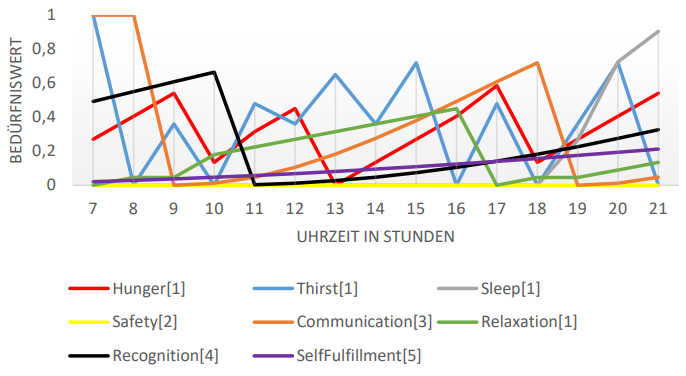
\includegraphics[scale=0.75]{images/schliecker_tagesablauf.PNG}
\caption{Regelbasierter Ansatz, Verlauf der durchschnittlichen Bedürfniswerte}
\label{fig:schliecker_tagesablauf}
\end{figure}

Aus der Verwendung von Regeln ergibt sich theoretisch ein statisches Verhalten, das unter Umständen vorhergesagt werden kann. Da es sich in der Simulation aber um Hintergrundcharaktere mit definierten Aktionen handelt, fallen diese statischen Eigenschaften nicht auf. Da die Bedürfnisse des Agenten nach außen hin nicht sichtbar sind, verhalten sich die Agenten zunächst ähnlich wie die trainierten NPCs. In der Abbildung \ref{fig:rulebased_day_cycle} werden die Verläufe der Bedürfnisse gezeigt, die sich beim regelbasierten Ansatz ergeben. Weiterhin zeigt die Abbildung \ref{fig:action_amounts_manual_vs_ril} einen Vergleich der Häufigkeiten der gewählten Aktionen zum \ac{reinforcement_learning}-Ansatz.

\begin{figure}[H]
\centering
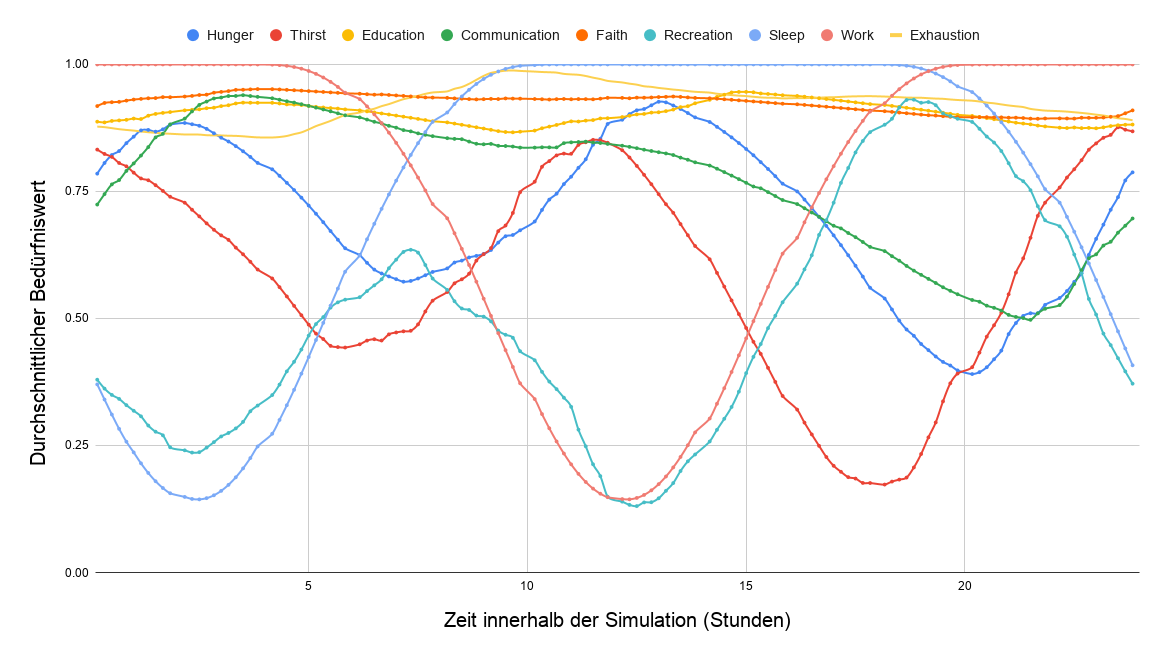
\includegraphics[scale=0.37]{images/rulebased/rulebased_day_cycle.png}
\caption{Regelbasierter Ansatz, Verlauf der durchschnittlichen Bedürfniswerte}
\label{fig:rulebased_day_cycle}
\end{figure}


\begin{figure}[H]
\centering
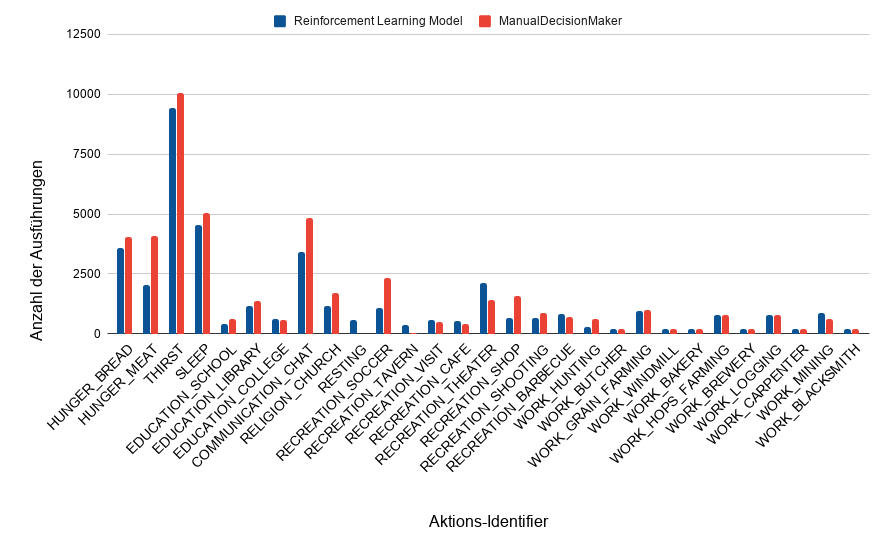
\includegraphics[scale=0.5]{images/training/action_amounts_manual_vs_ril.png}
\caption{Häufigkeiten der Aktionen, regelbasierter Ansatz und ML-Agents-Ansatz}
\label{fig:action_amounts_manual_vs_ril}
\end{figure}

Die beiden Abbildungen zeigen, dass sich insgesamt ein ähnliches Verhalten entwickelt hat. Ein ähnlicher Tagesablauf ist entstanden und die Häufigkeiten der gewählten Aktionen für beide Ansätze weisen hohe Gemeinsamkeiten auf. Erst sobald man einen regelbasierten NPC für einen längeren Zeitraum näher betrachtet, wird klar, dass sein Verhalten durch statische Regeln beeinflusst wird, da Aktionen sofort ausgelöst werden, sobald bestimmte Bedürfniswerte erreicht wurden. In einem realen Spiel kennt der Spieler die Bedürfnisse der Agenten jedoch nicht. Weiterhin handelt es sich hier um Hintergrundcharaktere. In der Regel würde ein Spieler keine Hintergrundcharaktere für eine so lange Zeit beobachten, dass ihm dieses statische Verhalten aufhalten könnte. Der Vorteil aus der Nutzung von Reinforcement Learning ist in diesem Fall also limitiert, da auch ein regelbasierter Ansatz zu einem akzeptablen Ergebnis führt. Der größte Vorteil ergibt sich vielmehr aus der Tatsache, dass die Agenten Entscheidungen aufgrund von sich verändernden Bedürfnissen treffen, die wiederum eine Auswirkung auf die Bedürfnisse des Agenten haben. Dadurch wird glaubwürdig das menschliche Verhalten imitiert.
Die Nutzung von Reinforcement Learning bietet jedoch Vorteile über das eigentliche Verhalten der Agenten hinaus an. Zwar ist der Ansatz mit einem höheren initialen Aufwand verbunden, doch resultiert daraus ein Verfahren, das sehr gut erweiterbar ist. Da der Trainingsvorgang die Auswahl von Aktionen übernimmt, können nun leicht neue Aktionen und Bedürfnisse hinzugefügt werden. Der initiale Aufwand für die Erzeugung eines regelbasierten Ansatzes ist geringer, allerdings ist dabei eine geringere Erweiterbarkeit gegeben. Je mehr Regeln definiert werden müssen, desto höher ist zudem die Wahrscheinlichkeit, dass Regeln sich widersprechen oder durch die hohe Anzahl Fehler im Programmcode eingebaut werden. Weiterhin muss stets eine Priorisierung von Bedürfnissen vorgenommen werden, was im \ac{reinforcement_learning}-Prozess automatisiert und intrinsisch passiert. Der Lernvorgang übernimmt in gewisser Weise die beim \ac{reinforcement_learning}-Ansatz die Definition der Regeln.


Für beide verwendete Ansätze ergibt sich eine hohe Skalierbarkeit, da Entscheidungen pro Agent in einem Abstand von mehreren Sekunden getroffen werden müssen. Die zusätzlich erforderliche Leistung der Nutzung einer höheren Anzahl von Agenten ist daher überschaubar. In einem Test wurden bis zu 1.000 Agenten innerhalb des Dorfes verwendet, die zwar die Kapazitätsgrenzen der Gebäude in der Stadt deutlich überschreiten, aber ohne drastische Performanceverluste dargestellt werden können. 

\chapter{Fazit}\label{fazit}
In diesem abschließenden Kapitel wird zunächst eine Zusammenfassung der weiteren Kapitel und der Ergebnisse der Arbeit vorgenommen. Darauf folgen eine Bewertung und eine Analyse von Problemen mit Machine Learning in Spielen sowie spezifischen Problemen des entwickelten Verfahrens. Ein Ausblick bildet anschließend den Abschluss der Arbeit.


\section{Zusammenfassung}\label{zusammenfassung}
Im ersten Kapitel wurde nach einer Einleitung in das Thema mit einer Vorstellung der Beweggründe für die Arbeit die allgemeine Idee der Thesis vorgestellt, die die Entwicklung einer Dorfsimulation beinhaltet, die auf Reinforcement Learning basiert.

Mehrere Grundlagenkapiteln vermittelten anschließend nötiges Basiswissen. Zunächst wurde auf die Entwicklung intelligenter Agenten in Videospielen eingegangen. Es folgte ein Überblick über mögliche Technologien zur Implementierung intelligenter Agenten. Die vorgestellten Technologien wurden im Einzelnen erläutert.

Anschließend folgte eine Einführung in das Reinforcement Learning mit einer umfassenden Vorstellung des Verfahrens und einer Rekapitulation der grundlegenden Vorgehensweise von Machine Learning. Auch mathematische Aspekte wurden beispielsweise durch die Erläuterung von Markov-Entscheidungsproblemen berücksichtigt. Verschiedene modellfreie und modellbasierte Algorithmen für die Implementierung von Reinforcement Learning wurden anschließend beschrieben. 

Im nächsten Kapitel wurden einige Beispiele für die Nutzung von Machine Learning in Spielen vorgestellt. Diese Beispiele verdeutlichten das Potential von Machine Learning im Bereich der Videospiele. Es wurde gezeigt, dass in diesem Bereich bereits erfolgreiche Projekte existieren, die Machine Learning nutzen, und dass dadurch das Spielerlebnis verbessert werden kann.

Im anschließenden Kapitel wurden durch die Vorstellung des verwendeten Frameworks Grundlagen für die Implementierung der Dorfsimulation geschaffen. Ein Beispielprojekt wurde implementiert, das die grundlegende Struktur und den Umgang mit dem Framework verdeutlicht.

Anschließend wurde die Implementierung der Dorfsimulation vorgestellt. Zunächst wurden dafür Anforderungen aufgestellt. Danach folgte eine Beschreibung der nötigen Modellierung des Dorfes. Die grundlegende Architektur und das Software-Design der Anwendung wurde beschrieben. Schließlich wurde die Implementierung anhand der einzelnen Klassen und Komponenten der Simulation umfassend erläutert.

Im nächsten Kapitel folgte die Beschreibung des Trainingsvorgangs für das in der Simulation genutzte Reinforcement Learning-Verfahren. Dabei wurde der generelle Ablauf des Trainings und die Auswahl der optimalen Hyperparameter ausführlich beschrieben. Verschiedene Metriken dokumentierten dabei das entstandene Verhalten der Agenten. Es wurde gezeigt, dass die Agenten sich sinnvoll verhalten.

Schließlich wurden zwei weitere entwickelte Ansätze für die Nutzung intelligenter Agenten in der Dorfsimulation, die nicht auf Machine Learning basieren, vorgestellt. Ein Vergleich der drei Ansätze wurde angefertigt.















\section{Bewertung}
In der vorliegenden Arbeit sollte ein neuer Ansatz für die Erzeugung glaubwürdiger NPCs in Videospielen vorgestellt werden, die über menschliche Bedürfnisse verfügen und diese als Grundlage für einen intelligenten Entscheidungsprozess nutzen. Mithilfe von Reinforcement Learning sollten die Agenten lernen, ihre Bedürfnisse zu maximieren. Dadurch sollte ein authentisches Verhalten erreicht werden, dass die NPCs menschlicher wirken lässt.
Dieser Ansatz wurde anhand einer Dorfsimulation umgesetzt, in der NPCs leben. Diese NPCs verfügen über Bedürfnisse und nutzen diese als Grundlage für ihre Entscheidungsfindung, die mit Reinforcement Learning implementiert wurde. Insgesamt ergibt sich dadurch ein lebendiges Dorf, das mit überzeugenden Agenten gefüllt ist. Die grundsätzlichen Ziele der Arbeit wurden damit erfüllt. 

In der Einleitung der Thesis wurde von statischen NPCs gesprochen, die in stets gleiche Verhaltensmuster verfallen, wie beispielsweise in \Fachbegriff{The Witcher 3} oder \Fachbegriff{The Elder Scrolls V: Skyrim}. In \Fachbegriff{The Witcher 3} werden für die Befüllung der Welt Hintergrundcharaktere verwendet, die jedoch über keine Persönlichkeit verfügen, sondern je nach Bedarf erzeugt werden, um eine bestimmte Aktion wieder und wieder auszuführen. In \Fachbegriff{The Elder Scrolls V: Skyrim} werden keine namenlosen Hintergrundcharaktere verwendet, doch auch hier demonstrieren die Agenten häufig kein intelligentes Verhalten.
Mit dem entwickelten, bedürfnisbasierten Ansatz ist eine Anwendung entstanden, die eine Mischung aus den beiden genannten Ansätzen für NPCs darstellt. Effektiv handelt es sich um Hintergrundcharaktere, die eine Umgebung mit Leben befüllen sollen. Ab dem Startzeitpunkt der Anwendung wird jedoch eine feste Anzahl von Agenten verwendet, die bis zum Beenden der Anwendung bestehen bleibt, sodass diese nicht nach Bedarf hinzugefügt und entfernt werden können. Alle NPCs verfügen über eine begrenzte eigene Persönlichkeiten, die durch Attribute beschrieben werden, und einen persistenten Wohnort.

Im Unterschied zu den genannten Beispielen ergibt sich für die entwickelten Agenten jedoch ein weniger statisches Verhalten. Stattdessen treffen die Agenten kontinuierlich Entscheidungen, die nicht auf Scripting, sondern auf ihren aktuellen Bedürfnissen beruhen. Dadurch, dass NPCs unterschiedlichen Berufen nachgehen und ihre Freizeitaktivitäten auf Basis ihrer persönlichen Präferenzen wählen, wird ein dynamisches Verhalten erreicht. Da ihre Aktionen auf menschlichen Eigenschaften basieren und die Agenten eigenständig einen Tagesablauf entwickelt haben, wirken ihre gewählten Entscheidungen glaubwürdig. Insgesamt erweckt das Dorf einen belebten Eindruck und die Agenten wirken authentisch.
Das dynamischere Verhalten der Agenten ist nicht nur auf Reinforcement Learning, sondern auch zu großen Teilen auf die Bedürfnisorientierung der Agenten zurückzuführen.
Im Abschnitt \ref{vergleich_verhalten} wurde gezeigt, dass auch durch einen regelbasierten Ansatz ein Verhalten entstehen kann, das bis zu einem gewissen Grade ausreichend dynamisch ist, wenn bedürfnisorientierte Agenten verwendet werden. Aufgrund des initial niedrigeren Aufwands eines solches Verfahrens spricht diese Tatsache nicht für die Verwendung von Reinforcement Learning. Allerdings ergibt sich dadurch auch eine hohe Erweiterbarkeit der Anwendung, da der Entscheidungsprozess der Agenten durch das Modell übernommen wird und nicht explizit definiert werden muss, wodurch mehr Aufwand und Fehler entstehen können. Die hohe Erweiterbarkeit bietet nicht nur einen Vorteil gegenüber regelbasierten Ansätzen, sondern auch für weitere klassische Verfahren für die Entwicklung intelligenter Agenten, wie zum Beispiel Finite State Machines. Auch hier führt das Einführen neuer Aktionen und Bedürfnisse oder die Veränderung von bestehenden Komponenten zu einem höheren Entwicklungsaufwand und einer höheren Fehleranfälligkeit, da der Entwickler die eigentliche Entscheidungsfindung im Gegensatz zum Reinforcement Learning selbst implementieren muss.   
Insgesamt wurde außerdem gezeigt, dass Reinforcement Learning eine Alternative für die Entscheidungsfindung von NPCs darstellt. Durch eine hohe Erweiterbarkeit bieten sich Vorteile gegenüber den in Kapitel \ref{intelligente_agenten} genannten klassischen Verfahren. Insgesamt kann außerdem ein dynamischeres, authentischeres Verhalten erreicht werden, das nicht auf fest definierten Regeln beruht. Dafür muss ein häufig zeitintensiver Trainingsvorgang in Kauf genommen werden, dessen Ergebnis vorher nicht bekannt ist und der für jede Änderung des Programmcodes erneut ausgeführt werden muss.










\subsection{Probleme mit Machine Learning und Reinforcement Learning}
Im folgenden Abschnitt wird auf generelle Probleme aufmerksam gemacht, die sich aus der Verwendung von Machine Learning für intelligente Agenten ergeben. Weiterhin werden Probleme beschrieben, die während der Arbeit angetroffen wurden.

\subsection{Beschaffenheit des Aktionsraumes}\label{allgemeine_aktionen}
Die Art und Weise, in der Reinforcement Learning im Kontext dieser Thesis verwendet wurde, unterscheidet sich teilweise von den klassischen Anwendungsformen der Technologie. In typischen Anwendungsszenarien gibt es einen Agenten in einer Umgebung, in der die Kombination von beliebigen, unterschiedlichen Aktionen zu einem Ziel führt, das der Agent erreichen muss. Es ist nicht garantiert, dass jede Aktion des Agenten eine Belohnung oder eine Bestrafung zur Folge hat. Der Agent lernt, in Abhängigkeit seiner Zustandsvariablen eine Strategie zu entwickeln, die zu einem ganz bestimmten Ziel führt. In der Dorfsimulation hingegen gibt es solche Ziele nicht. Während des Trainingsvorgangs wird dort die laufende Episode nach einer beliebigen Anzahl ausgeführter Aktionen unterbrochen, anstatt nach dem erfolgreichen Erreichen eines Ziels. Statt durch das Erreichen eines Ziels führt hier jede einzelne Aktion zu einer Belohnung oder einer Bestrafung aufgrund der Bedürfnisse des Agenten. Die Aktionen, die dem Agenten zur Verfügung gestellt werden, sind dabei durch ActionPlans genau vorgegeben und beinhalten bereits exakt beschriebene Abläufe. In der Regel werden jedoch viel allgemeinere Aktionen vorgegeben, wie beispielsweise in der in Kapitel \ref{ml_unity} vorgestellten Beispielimplementierung für die Lösung eines Problems durch das ML-Agents-Framework. Dort wurden lediglich die Aktionen \Fachbegriff{rechts/links bewegen} und \Fachbegriff{vorwärts/rückwärts bewegen} definiert, bis der Agent schlussendlich sein Ziel erreicht. Durch die Definition von allgemein gehaltenen Aktionen ermöglicht man es dem Agenten, eine eigene Strategie zu entwickeln. So entsteht die theoretische Möglichkeit, komplexe Muster, die vor dem Trainingsvorgang nicht bekannt waren, erlernen zu können. In einem Projekt der Firma OpenAI, in dem Agenten sich vor anderen Agenten verstecken müssen, wurde zum Beispiel gezeigt, dass mithilfe von simplen Aktionen wie \Fachbegriff{Schieben} und \Fachbegriff{Bewegen} äußerst komplexes Verhalten erreicht werden kann \cite{hide_and_seek_openai} \cite{hide_and_seek_openai_paper}. Ohne jegliche Instruktionen haben die sich versteckenden Agenten sogar gelernt, ihre Umgebung so zu manipulieren, dass sie sich selbst in einem Käfig von Objekten einsperren, damit sie von den suchenden Agenten nicht gefunden werden können. 
Auch in der Dorfsimulation lernen die Agenten erfolgreich, eine Belohnungsfunktion zu maximieren. Durch die exakte Vorgabe und Beschreibung der möglichen Aktionen durch ActionPlans wird ihnen jedoch die Möglichkeit genommen, komplexere Verhaltensmuster zu entwickeln. Man entzieht den Agenten sozusagen ihre \Fachbegriff{Kreativität}, indem genaue Vorgaben gemacht werden. Ein wirklicher Lernvorgang im Bezug auf das intelligente Erlernen von Verhaltensmustern ist hier weniger gegeben. Stattdessen findet eher ein rein mathematischer Vorgang statt, indem Beziehungen zwischen Bedürfnissen und gesammelten Belohnungen gefunden werden.

Für die Entwicklung der Entscheidungsfindung von Hintergrundcharakteren ist das gewählte Verfahren trotzdem angemessen. Wenn alle Teilaktionen der ActionPlans in einzelne Aktionen konvertiert oder generell ein Aktionsraum mit einem deutlich höheren Level von Abstraktion gewählt worden wäre, hätte das die Komplexität des Problems deutlich erhöht und damit das Training erschwert. Beispielsweise war für das Training des genannten Versteckspiels der Firma OpenAI ein 98,8 Stunden langer Trainingsvorgang mit 167,4 Millionen abgeschlossenen Episoden nötig, bis eine Konvergenz des Modells erreicht wurde \cite{hide_and_seek_openai_paper}. OpenAI Five wurde sogar über mehrere Monate hinweg unter großem Hardwareaufwand trainert, bis übermenschliches Verhalten erreicht werden konnte \cite{openai_five_paper}. Es muss daher ein Kompromiss aus der \Fachbegriff{Intelligenz} der Agenten, den Möglichkeiten des Entwicklers und den Anforderungen gefunden werden.




\subsection{Dauer der Trainingsvorgänge}
Wie im vorherigen Abschnitt erwähnt, ist ein großes Problem bei der Entwicklung von Agenten mittels Machine Learning die notwendige Zeit, die für das Training und die Feinabstimmung von Belohnungen und Hyperparametern aufgewendet werden muss. Entscheidungsbäume, State Machines oder weitere Verfahren (siehe Kapitel \ref{intelligente_agenten}) verlangen zwar unter Umständen mehr Zeit für die eigentliche Implementierung des Programmcodes, danach ist die Entwicklung der Agenten jedoch größtenteils abgeschlossen. Wenn Machine Learning-Verfahren wie Reinforcement Learning verwendet werden, muss auch nach der Anfertigung des Programmcodes noch Zeit und Rechenleistung investiert werden, um die Agenten effektiv zu trainieren. Hier muss also klar erörtert werden, was die eigentlichen Anforderungen an die Anwendung sind. Wenn keine hohen Voraussetzungen an die Intelligenz der Agenten gestellt werden, ist die Wahl einer State Machine mit hoher Wahrscheinlichkeit sinnvoller als die Nutzung von Reinforcement Learning. Wenn die Agenten jedoch den Eindruck erwecken sollen, sich an bestimmte Situationen anpassen zu können und generell kluge Entscheidungen treffen sollen, kann Machine Learning einen großen Vorteil darstellen. OpenAI hat mit der Entwicklung von \Fachbegriff{OpenAi Five} gezeigt, dass durch eine durchdachte Anwendung von Reinforcement Learning übermenschliche Leistungen erbracht und Agenten mit extrem intelligentem Verhalten entwickelt werden können \cite{openai_five} (siehe Abschnnitt \ref{aktuelle_entwicklungen_rl}). Um diese Erfolge möglich zu machen, waren jedoch ebenfalls eine große Menge von Hardware und Zeit erforderlich. Die Dauer des Trainings stellt also ein grundlegendes Problem dar.
In der vorliegenden Arbeit bestand ebenfalls die Schwierigkeit, dass viele Trainingsvorgänge durchgeführt werden mussten. Dieses Verfahren beschreibt keine Notwendigkeit, sondern dient vielmehr zur Auffindung des optimalen Ergebnisses durch die Erzeugung einer Policy mit der höchsten Gesamtbelohnung und dem besten resultierenden Agentenverhalten. Ein weiterer legitimer Ansatz wäre es gewesen, das erste \Fachbegriff{brauchbare} Modell zu akzeptieren, das annehmbare Ergebnisse für das Verhalten der Agenten hervorbringt.

Weiterhin bringt die Verwendung der GPU für Berechnungen im neuronalen Netz keine Vorteile. Der limitierende Faktor ist nicht das Netz selbst, sondern die in Unity laufende Simulation, die einen großen Overhead erzeugt. Durch die parallele Verwendung mehrerer Dörfer kann dieses Problem nur bis zu einem gewissen Grad reduziert werden.

\subsection{Nichtdeterminismus als Hindernis}
Aus der Nutzung von Machine Learning resultiert unweigerlich ein nichtdeterministisches Verhalten. Für die Entwicklung von NPCs stellt das ein Problem dar. Wenn für ein Spiel Agenten entwickelt werden, mit denen der Spieler interagieren kann, so agieren diese typischerweise deterministisch. In den meisten Spielen müssen bestimmten Regeln verfolgt werden, damit Game Designer und Entwickler das Verhalten der Agenten vorhersagen und auf bestimmte Situationen anpassen können. Die Agenten müssen leicht zu kontrollieren sein und über ein verlässliches und vorhersehbares Verhalten verfügen. Game Designer haben klare Vorstellungen für das Verhalten eines NPC. Wenn dieser nicht über genau das modellierte Verhalten verfügt, behindert das die Entwicklung des Spiels.
Daher erscheint es nicht möglich, das gesamte Verhalten eines komplexen NPCs mit Verfahren wie Reinforcement Learning zu modellieren - es sei denn es handelt sich um Hintergrundcharaktere, wie in dieser Thesis. Diese dienen hauptsächlich zum Befüllen der Welt, sodass sie kein konkretes Verhalten an den Tag legen müssen. 

Machine Learning-Verfahren stellen häufig eine \sogenannt{Black Box} dar. Der genaue Entscheidungsprozess des Verfahrens ist für den Entwickler daher nicht immer nachvollziehbar, sodass das resultierende Verhalten nicht genau vorhergesagt werden kann. Stattdessen müssen Nicht-Hintergrund-NPCs jedoch kontrollierbar und berechenbar sein. Wenn ein NPC zum Beispiel für das Storytelling eines Spiels relevant ist, dann muss er sich auch immer so verhalten, wie der Game Designer, der die Geschichte entwirft, es vorsieht. Statt des gesamten Verhaltens des NPCs könnte nur ein Teil davon durch Machine Learning geregelt werden. So könnte er etwa Entscheidungen aufgrund von Bedürfnissen treffen, sobald er sich in einem Idle-Modus befindet und aktuell nicht für andere Komponenten des Spiels benötigt wird.





\subsection{Probleme mit ML-Agents}
Während der Implementierung der Dorfsimulation kam es zu Problemen mit dem ML-Agents Framework, besonders während der Ausführung der Trainingsvorgänge. Ein bekanntes Problem bei der Nutzung des Frameworks unter Windows ist, dass das Training aus unbekannten Gründen anhält. Dieser Fehler kommt häufig vor, wenn das Training im Hintergrund ausgeführt wird, also wenn das entsprechende Fenster minimiert ist. Der Vorgang kann dann wieder gestartet werden, indem das Fenster geöffnet und eine beliebige Taste gedrückt wird.
Da für das Training ohnehin viel Zeit investiert werden muss, stellt dieses Problem einen stark störenden Faktor dar.

Ähnliche Probleme entstehen, wenn ein Trainingsvorgang mit einer exportierten Unity-Anwendung läuft und zeitgleich im Unity-Editor gearbeitet wird. Das Training stürzt dann manchmal vollständig ab, auch im Editor kommt es zu Fehlermeldungen. Da es sich bei dem Framework noch um eine Beta-Version handelt, sind Fehler allerdings zu erwarten.

















\section{Ausblick}\label{ausblick}
In diesem Abschnitt werden weitere, zukünftige Möglichkeiten zur Verbesserung der entwickelten Agenten und zur Anwendung von Machine Learning in Spielen vorgeschlagen.

Die entwickelte Dorfsimulation beinhaltet Agenten, die individuell handeln. Sie haben kein Gemeinschaftsgefühl, sondern kennen lediglich ihre eigenen Bedürfnisse. Interessant wäre die Entwicklung eines Gemeinschaftsgefühls, sodass die Agenten auf gemeinsame Ziele hinarbeiten.
Für das Projekt OpenAI Five (siehe Abschnitt \ref{aktuelle_entwicklungen_rl}) wurde ein Hyperparameter \Fachbegriff{team spirit} eingeführt, sodass Agenten von den Belohnungsfunktionen anderer Agenten beeinflusst werden \cite{openai_five}. Die Erfolgsquote der Agenten konnte damit stark verbessert werden. Die Nutzung eines solchen Konzepts in einem Dorfsystem könnte dazu führen, dass Agenten für ein übergeordnetes Ziel zusammenarbeiten oder sich gegenseitig helfen.

Wenn eine sinnvoller Ansatz für die Implementierung eines Ressourcensystems gefunden wird, könnten außerdem mehrere Dörfer parallel verwendet werden, die miteinander interagieren können. Interessant wären nun die möglichen Auswirkungen eines Gemeinschaftsgefühls, wie oben beschrieben. Dadurch könnte der Versuch der Agenten entstehen, den Erfolg des eigenen Dorfes zu steigern. Durch Interaktionen zwischen den Dörfern wie Handel oder Krieg könnten dann interessante Verhaltensweisen entstehen.

Um die Entwicklung von komplexeren Verhaltensmustern anzuregen, könnten allgemeinere Aktionen für die Agenten definiert werden, wie in Abschnitt \ref{allgemeine_aktionen} vorgeschlagen. Das würde zwar die Komplexität des zugrunde liegenden Optimierungsproblems erhöhen, aber gleichzeitig die Möglichkeit bieten, ein intelligenteres Verhalten entstehen zu lassen. Interessant wäre es, dem Agenten auch die Navigation innerhalb des Dorfes zu überlassen, ähnlich wie im vorgestellten Beispiel in Kapitel \ref{ml_unity}. Bestimmte Aktionen würden dann erst verfügbar sein, wenn der Agent sich in der Nähe eines Gebäudes befindet. In diesem Fall müssten bestimmte Variablen in den Vektor von Observations mit aufgenommen werden, wie die Orte im Umkreis des Agenten und deren Positionen sowie der Position des Agenten.

Vorstellbar wäre auch die Entwicklung eines Ökosystems, in dem sich neben Dorfbewohnern auch Tiere aufhalten, die primitive Bedürfnisse erfüllen müssen. Beispielsweise könnten Jäger aus dem Dorf diese Tiere jagen, wobei die Tiere versuchen zu überleben.

Insgesamt könnte man äußere Einflüsse in Simulationen integrieren. Um ein absolut glaubhaftes Verhalten der Dorfbewohner zu erzeugen, müssen diese auf Aktionen des Spielers und auf Umstände aus der Umgebung reagieren. Diese sind nicht Teil der Arbeit, da es sich nicht um ein Spiel handelt, sondern um eine Simulation, in der die Bedürfnisse der Agenten im Vordergrund stehen. Zum Beispiel könnte es die Möglichkeit geben, dass sich Wetterbedingungen und Jahreszeiten verändern. Dies hätte etwa Auswirkungen auf die Ernte, sodass die NPCs lernen müssen, andere Nahrungsquellen zu finden oder im Sommer Vorräte anzuhäufen. Außerdem könnten die Agenten lernen, auf die Aktionen eines Spielers zu reagieren - zum Beispiel könnte dieser einen Diebstahl begehen oder einen Dorfbewohner angreifen. Hier könnte wieder das vorgeschlagene Gemeinschaftsgefühl genutzt werden. Eine weitere Möglichkeit besteht in der Implementierung von Moralvorstellungen, die abhängig von der Persönlichkeit eines Agenten sind.

Um das Verhalten der Agenten besser beurteilen zu können, wäre die parallele Ausführung von Agenten mit unterschiedlichen Verfahren zur Entscheidungsfindung denkbar. In diesem Fall würden zum Beispiel GOAP-Agenten, \ac{reinforcement_learning}-Agenten und regelbasierte Agenten in demselben Dorf leben, um einen einfachen Vergleich erstellen zu können.

Die meisten vorgeschlagenen Ideen gehen deutlich über die in dieser Arbeit entwickelten Möglichkeiten hinaus, bieten aber interessante Ansatzpunkte für weitere Forschungsarbeit. Dazu wäre voraussichtlich deutlich leistungsstärkere Hardware für den Trainingsvorgang nötig.

In den vorherigen Abschnitten wurde bereits gezeigt, dass Machine Learning sich nicht für die vollständige Modellierung des Verhaltens bestimmter NPCs eignet. Dazu gehören alle NPCs, die für den Spielfortschritt relevant sind und sich deterministisch verhalten müssen. Für diese Agenten könnten höchstens Teile ihrer Entscheidungsfindung dadurch implementiert werden. Stattdessen könnten zukünftig Verfahren wie Reinforcement Learning für die Entwicklung von Hintergrundcharakteren entwickelt werden. Besonders in Verbindung mit der Modellierung von menschlichen Eigenschaften wie Bedürfnissen ist die Kombination der Verfahren in diesem Anwendungsbereich vielversprechend. Auch in kompetitiven Online-Spielen zeigt Reinforcement Learning für die Zukunft ein hohes Potential.


\appendix

\chapter{Anhang A - Wahl der optimalen Hyperparameter}
Dieser Anhang beinhaltet die Dokumentation der Auswahl der optimalen Hyperparameter, die nicht zum gewünschten Erfolg geführt hat.


\subsection*{Lernrate}
Zunächst wurde die Lernrate angepasst. Neben der bereits definierten Lernrate von $4 * 10^{-4}$, beziehungsweise $4e-4$ in der Terminologie der ML-Agents-Konfigurationsdatei, wurden eine geringere Lernrate von $5e-5$ und eine höhere Lernrate von $8e-3$ verwendet. Die Ergebnisse sind in den folgenden Abbildungen zu erkennen.

\begin{figure}[H]
\centering
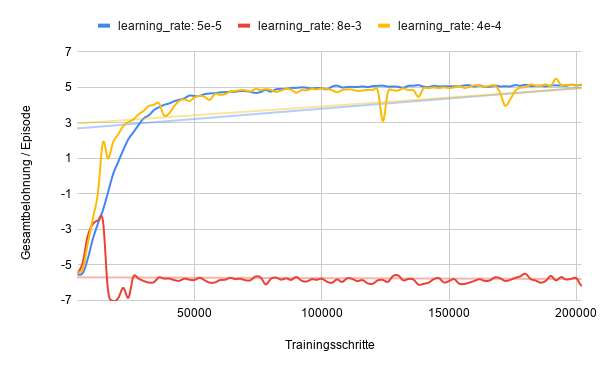
\includegraphics[scale=0.6]{images/training/base_results/result_learningrate_rewards.png}
\caption{Belohnungsverlauf, Anpassung von \Fachbegriff{learning\_rate}}
\label{fig:result_learningrate_rewards}
\end{figure}

\begin{figure}[H]
\centering
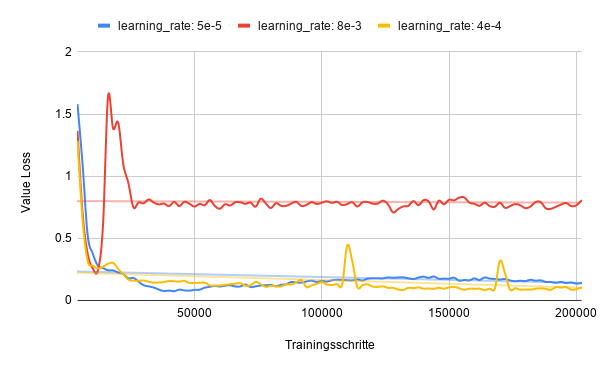
\includegraphics[scale=0.6]{images/training/base_results/result_learningrate_loss.png}
\caption{Verlauf des Value Loss, Anpassung von \Fachbegriff{learning\_rate}}
\label{fig:result_learningrate_loss}
\end{figure}

\begin{figure}[H]
\centering
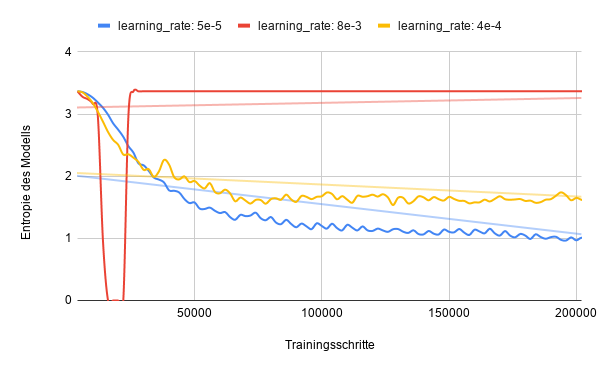
\includegraphics[scale=0.6]{images/training/base_results/result_learningrate_entropy.png}
\caption{Entropieverlauf, Anpassung von \Fachbegriff{learning\_rate}}
\label{fig:result_learningrate_entropy}
\end{figure}

Man erkennt deutlich, dass mit $8e-3$ eine deutlich zu hohe Lernrate gewählt wurde. Zwar steigt die Belohnungsfunktion anfangs im Vergleich leicht schneller, doch schließlich fällt die Kurve rapide ab und bleibt anschließend auf einem sehr schlechten Niveau. Es ist zu vermuten, dass durch den hohen Wert beim Gradientenaufstieg Maxima übersprungen werden. Die Policy wird also jeweils zu stark geändert. Das führt zu einem völlig unbrauchbaren Ergebnis. Auch anhand der Entropie und dem Value Loss wird dies deutlich.
Die Lernrate des Basistrainings mit dem Wert $4e-4$ führt zu einem deutlich besseren Ergebnis. Im Vergleich zu der Kurve mit einer Lernrate von $5e-5$ steigt sie schneller, weist jedoch zwischenzeitlich deutliche Einbrüche auf. Insgesamt wurde jedoch ein ähnlich gutes Ergebnis erzielt, da die Belohnungen nach etwa 100.000 Schritten fast identische Werte annehmen. Der Value Loss erreicht für die niedrigere Lernrate leicht schlechtere Ergebnisse, jedoch ist für die niedrige Lernrate auch zum Ende des Graphen hin eine Abnahme zu erkennen, während der Graph der mittelhohen Lernrate ein Plateau erreicht. Daher wird davon ausgegangen, dass sich der Value Loss mit einer höheren Anzahl von Trainingsschritten weiter verbessert.
Die Entropie zeigt deutlich, dass mit der geringeren Lernrate weniger zufällige Entscheidungen getroffen werden. Aufgrund dieser Tatsache und der deutlich höheren Stabilität der Belohnungsfunktion wird die Lernrate für das finale Training auf den Wert $5e-5$ festgelegt. Generell ist anzunehmen, dass mit einer geringeren Lernrate stets mindestens äquivalente Ergebnisse erzeugt werden können, sich aber insgesamt ein stabileres Training ergibt. Die Anzahl der Trainingsschritte kann dabei problemlos erhöht werden. Die höhere Steigung der Belohnungsfunktion für die mittelhohe Lernrate ist nicht relevant - das Endergebnis und die Stabilität des Trainings spielen eine höhere Rolle.


\subsection*{Anzahl der Schichten}
Weiterhin wurde die Anzahl der Schichten im neuronalen Netz angepasst. Das Basistraining beinhaltet ein Netz mit drei Schichten. Zusätzlich wurden zwei, vier und fünf Schichten getestet.

\begin{figure}[H]
\centering
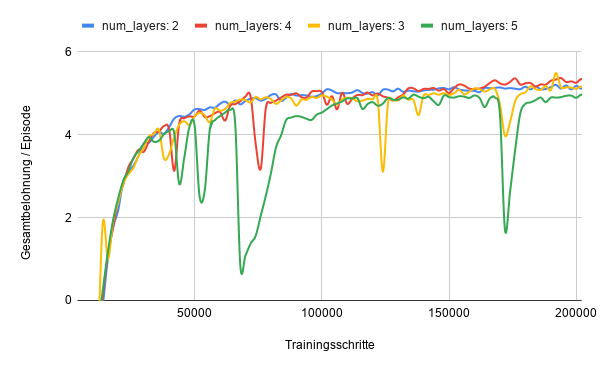
\includegraphics[scale=0.6]{images/training/base_results/result_layers_reward.png}
\caption{Belohnungsverlauf, Anpassung von \Fachbegriff{num\_layers}}
\label{fig:result_layers_reward}
\end{figure}

\begin{figure}[H]
\centering
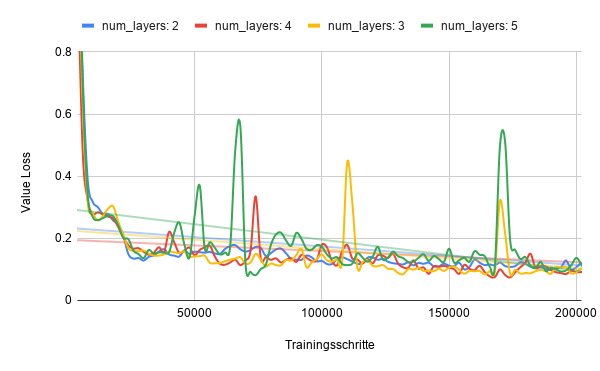
\includegraphics[scale=0.6]{images/training/base_results/result_layers_loss.png}
\caption{Verlauf des Value Loss, Anpassung von \Fachbegriff{num\_layers}}
\label{fig:result_layers_loss}
\end{figure}

\begin{figure}[H]
\centering
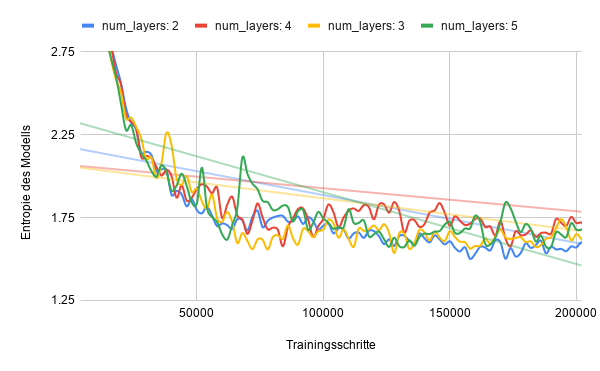
\includegraphics[scale=0.6]{images/training/base_results/result_layers_entropy.png}
\caption{Entropieverlauf, Anpassung von \Fachbegriff{num\_layers}}
\label{fig:result_layers_entropy}
\end{figure}

Anhand der Belohnungsfunktion kann man erkennen, dass die Verwendung von vier Schichten zu dem höchsten Reward führt. Insgesamt ist der allgemeine Verlauf der Funktionen ähnlich. Wenn allerdings fünf Schichten verwendet werden, entstehen starke Schwankungen und Einbrüche sowie eine insgesamt niedrigere Belohnung. Das lässt sich auch anhand des Entropieverlaufs und dem Value Loss erkennen. Die Nutzung von fünf Schichten ist daher nicht akzeptabel. Vier verwendete Schichten führen zu einem leicht erhöhten Entropieverlauf und einer Value Loss-Funktion, die sich mit den anderen Verläufen deckt. Da insgesamt aber eine höhere Belohnung erzielt wird, werden für das finale Training vier Schichten verwendet.   


\subsection*{Anzahl der Neuronen}
Die Anzahl der Neuronen wurde auf eine Anzahl von 128, 256, 384 und 512 festgelegt. Aufgrund der Erkenntnis des letzten Abschnitts wurden hierfür vier Schichten genutzt.

\begin{figure}[H]
\centering
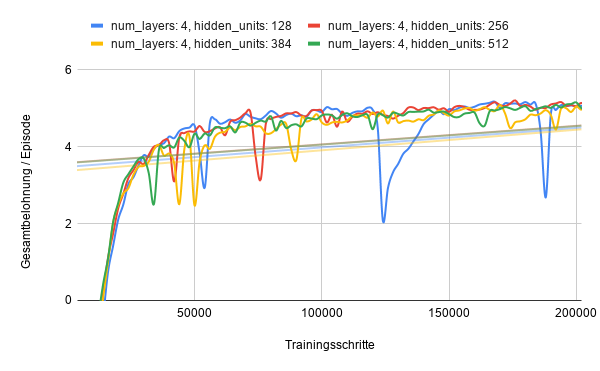
\includegraphics[scale=0.6]{images/training/base_results/result_neurons_rewards.png}
\caption{Belohnungsverlauf, Anpassung von \Fachbegriff{hidden\_units}}
\label{fig:result_neurons_rewards}
\end{figure}

\begin{figure}[H]
\centering
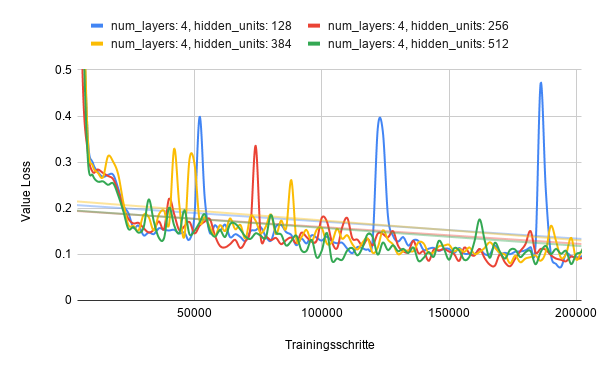
\includegraphics[scale=0.6]{images/training/base_results/result_neurons_loss.png}
\caption{Verlauf des Value Loss, Anpassung von \Fachbegriff{hidden\_units}}
\label{fig:result_neurons_loss}
\end{figure}

\begin{figure}[H]
\centering
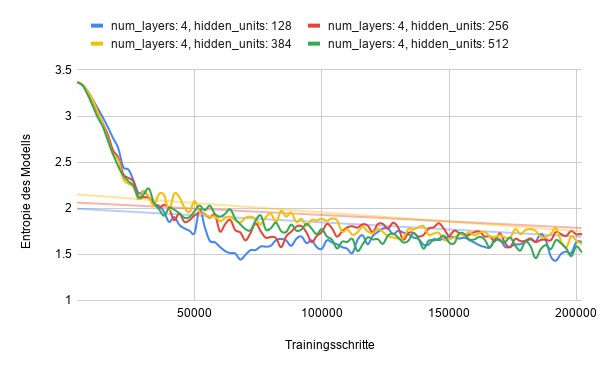
\includegraphics[scale=0.6]{images/training/base_results/result_neurons_entropy.png}
\caption{Entropieverlauf, Anpassung von \Fachbegriff{hidden\_units}}
\label{fig:result_neurons_entropy}
\end{figure}

An dem Verlauf der akkumulierten Belohnungen kann man erkennen, dass insgesamt sehr ähnliche Ergebnisse für die jeweils höchste Belohnung erzielt werden. Die Nutzung von 128 Neuronen pro Schicht führt allerdings zu häufigeren Einbrüchen, da durch die geringere Anzahl der Neuronen weniger kleinschrittige Änderungen des Modells möglich sind. 128 Neuronen sind daher nicht ausreichend. Für 384 und 512 Neuronen wird ein insgesamt leicht schlechteres und instabileres Ergebnis erreicht, als bei 256. Mit 384 Neuronen wurde also eine zu hohe Anzahl gewählt.

Die genannten Einbrüche mit 128 Neuronen sind ebenfalls in der Value Loss-Funktion zu betrachten. Die beiden Kurve für 256 und 384 Neuronen erreichen hingegen sehr ähnliche Ergebnisse. Ebenso ähneln sich deren Funktionen für die Entropie des Modells. Hier ist weiterhin zu erkennen, dass durch die Nutzung von weniger Neuronen eine schnellere Konvergenz erreicht wird, nach etwa 150.000 Trainingsschritten erreichen die Kurven jedoch ein ähnliches Level.
Es besteht zusätzlich die Vermutung, dass bei einer Erhöhung der Anzahl der Neuronen mehr Trainingsschritte benötigt werden, um das Modell hinreichend anzupassen. Daher wird ein erweiterter Trainingslauf in der folgenden Abbildung \ref{fig:result_neurons_rewards_extended} betrachtet:

\begin{figure}[H]
\centering
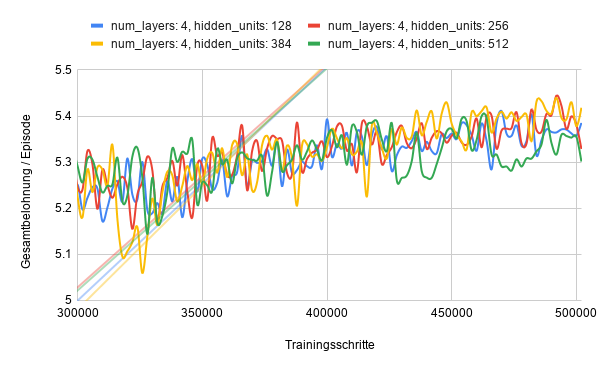
\includegraphics[scale=0.7]{images/training/base_results/result_neurons_rewards_extended.png}
\caption{Erweiterter Belohnungsverlauf, Anpassung von \Fachbegriff{hidden\_units}}
\label{fig:result_neurons_rewards_extended}
\end{figure}

In der Grafik ist zu erkennen, dass sich das Ergebnis für höhere Mengen von Neuronen mit steigender Anzahl von Trainingsschritten leicht verbessert. Aufgrund dieses Verlaufs und dem schlechteren Verlauf des Trainings mit 384 Neuronen werden insgesamt 256 Neuronen pro Schicht für das finale Training genutzt.


\subsection*{Rekurrentes Netz}
Der Parameter \Fachbegriff{use\_recurrent} wird auf \Fachbegriff{true} gesetzt, um ein rekurrentes neuronales Netz zu nutzen. Dabei wird eine \Fachbegriff{memory\_size} von der Größe $128$ genutzt. Die Ergebnisse sind in den folgenden Abbildungen zu sehen.

\begin{figure}[H]
\centering
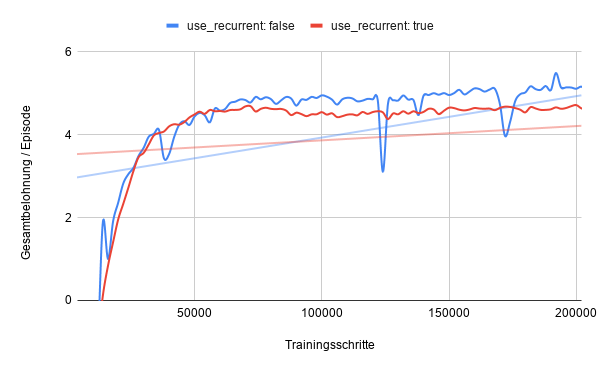
\includegraphics[scale=0.6]{images/training/base_results/result_userecurrent_rewards.png}
\caption{Belohnungsverlauf, Anpassung von \Fachbegriff{use\_recurrent}}
\label{fig:result_userecurrent_rewards}
\end{figure}

\begin{figure}[H]
\centering
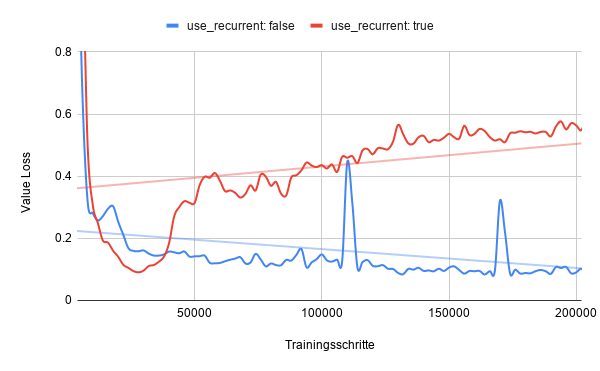
\includegraphics[scale=0.6]{images/training/base_results/result_userecurrent_loss.png}
\caption{Verlauf des Value Loss, Anpassung von \Fachbegriff{use\_recurrent}}
\label{fig:result_userecurrent_loss}
\end{figure}

\begin{figure}[H]
\centering
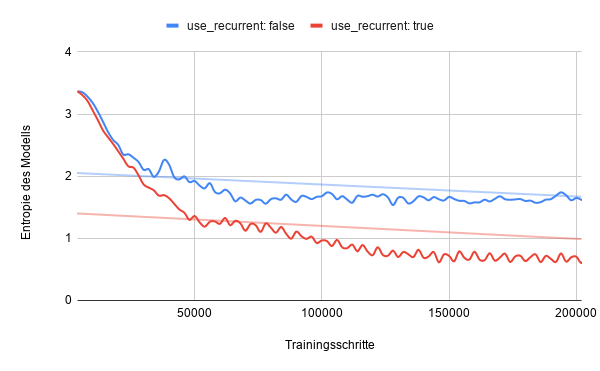
\includegraphics[scale=0.6]{images/training/base_results/result_userecurrent_entropy.png}
\caption{Entropieverlauf, Anpassung von \Fachbegriff{use\_recurrent}}
\label{fig:result_userecurrent_entropy}
\end{figure}

Insgesamt hat sich der Verlauf der Belohnungsfunktion stark verschlechtert. Die Kurve des Value Loss steigt nach einem initialen Abstieg stark an und erzielt schlussendlich ein extrem schlechtes Ergebnis. Zwar wird eine niedrigerer Wert für die Entropie erreicht, doch insgesamt ist das Ergebnis nicht akzeptabel. Daher wird von der Nutzung von rekurrenten Netzen abgesehen. Tatsächlich wurde durch das Training ein so viel schlechteres Ergebnis erzielt, dass von einer weiteren Anpassung der Parameter bezüglich rekurrenter Netze abgesehen wird.



\subsection*{Gamma}
Um den Einfluss zukünftiger Belohnungen auf die Entscheidungen des Agenten zu beeinflussen, wird der Parameter Gamma ($\gamma$) angepasst (siehe Abschnitt \ref{markov_decision_problems}). 

\begin{figure}[H]
\centering
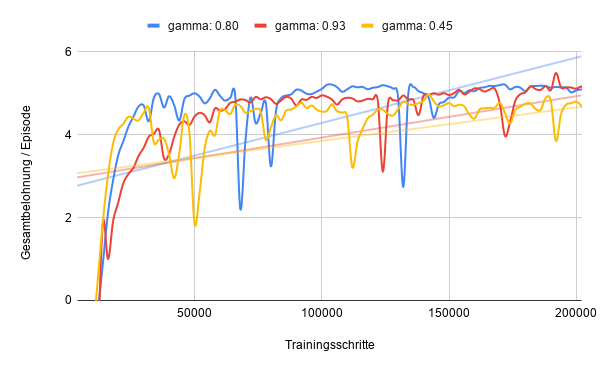
\includegraphics[scale=0.6]{images/training/base_results/result_gamma_rewards.png}
\caption{Belohnungsverlauf, Anpassung von \Fachbegriff{gamma}}
\label{fig:result_gamma_rewards}
\end{figure}

\begin{figure}[H]
\centering
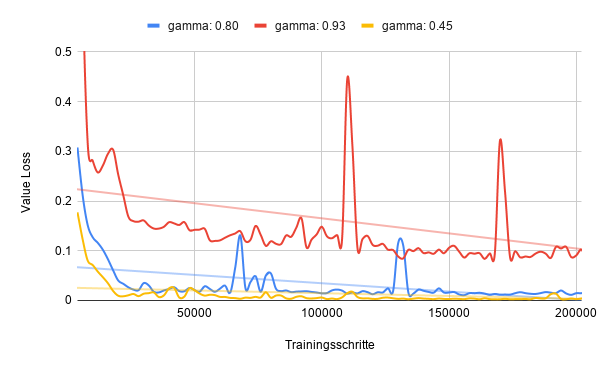
\includegraphics[scale=0.6]{images/training/base_results/result_gamma_loss.png}
\caption{Entropieverlauf, Anpassung von \Fachbegriff{gamma}}
\label{fig:result_gamma_loss}
\end{figure}

\begin{figure}[H]
\centering
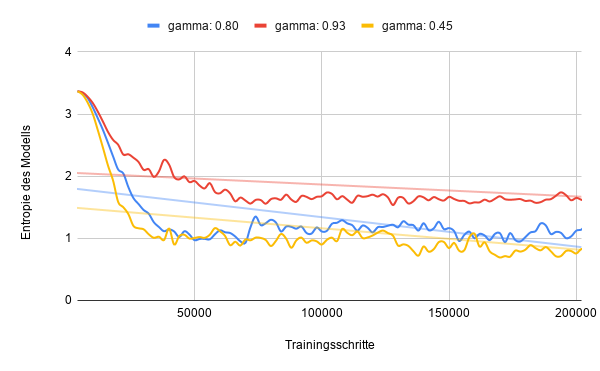
\includegraphics[scale=0.6]{images/training/base_results/result_gamma_entropy.png}
\caption{Verlauf des Value Loss, Anpassung von \Fachbegriff{gamma}}
\label{fig:result_gamma_entropy}
\end{figure}

An dem Entropieverlauf ist klar zu erkennen, dass die Wahl eines niedrigen Werts für $\gamma$ zu einem besseren Ergebnis führt. Ebenso verhält es sich mit der Entropie. Der Graph, der den niedrigsten Wert mit $\gamma = 0.45$ repräsentiert, zeigt das beste Ergebnis. Gleichzeitig erzielt der Trainingsvorgang mit diesem Wert deutlich schlechtere Werte für den Belohnungsverlauf. Das beste Ergebnis wird hier von dem Graphen erreicht, der durch den Wert $\gamma = 0.80$ entstanden ist. $\gamma$ wird daher auf diesen Wert festgelegt.



\subsection*{Größe der Batches}
Verschiedene Parameter innerhalb des empfohlenen Intervalls für den Parameter \Fachbegriff{batch\_size} wurden getestet. Die Ergebnisse sind im Folgenden zu erkennen:

\begin{figure}[H]
\centering
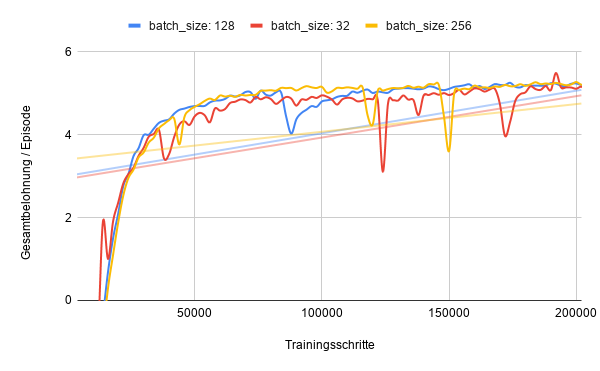
\includegraphics[scale=0.6]{images/training/base_results/result_batchsize_rewards.png}
\caption{Belohnungsverlauf, Anpassung von \Fachbegriff{batch\_size}}
\label{fig:result_batchsize_rewards}
\end{figure}

\begin{figure}[H]
\centering
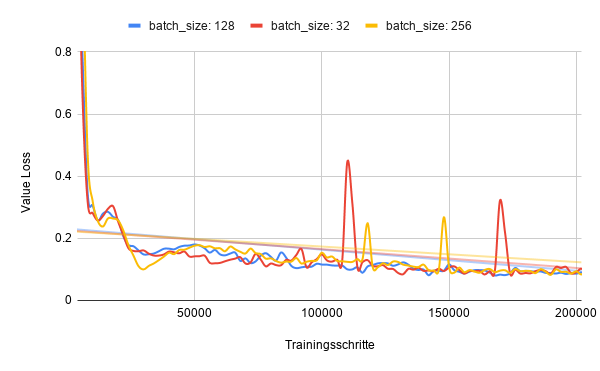
\includegraphics[scale=0.6]{images/training/base_results/result_batchsize_loss.png}
\caption{Verlauf des Value Loss, Anpassung von \Fachbegriff{batch\_size}}
\label{fig:result_batchsize_loss}
\end{figure}

\begin{figure}[H]
\centering
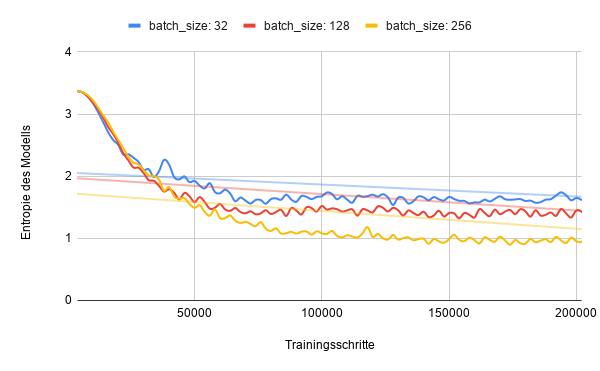
\includegraphics[scale=0.6]{images/training/base_results/result_batchsize_entropy.png}
\caption{Entropieverlauf, Anpassung von \Fachbegriff{batch\_size}}
\label{fig:result_batchsize_entropy}
\end{figure}

Es ist deutlich zu erkennen, dass sich für die höchste \Fachbegriff{batch\_size} die am wenigsten zufälligen Entscheidungen ergeben. Die Verläufe der Value Loss- und Belohnungsfunktionen sind weitestgehend identisch. Daher wird eine Batchgröße von 256 gewählt.



\subsection*{Beta}
Weiterhin wurden verschiedene Wert für den Parameter Beta ($\beta$) ausprobiert. Das Resultat ist in den folgenden Abbildungen erkennbar:

\begin{figure}[H]
\centering
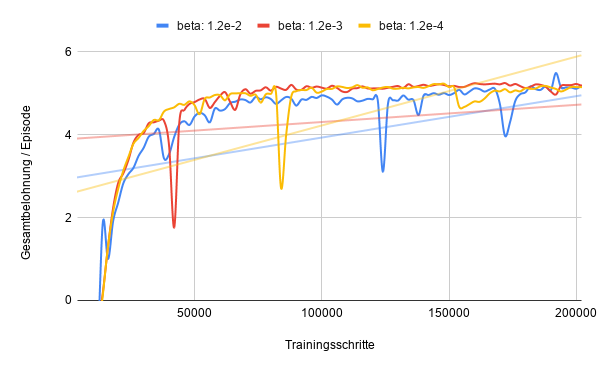
\includegraphics[scale=0.6]{images/training/base_results/result_beta_rewards.png}
\caption{Belohnungsverlauf, Anpassung von \Fachbegriff{beta}}
\label{fig:result_beta_rewards}
\end{figure}

\begin{figure}[H]
\centering
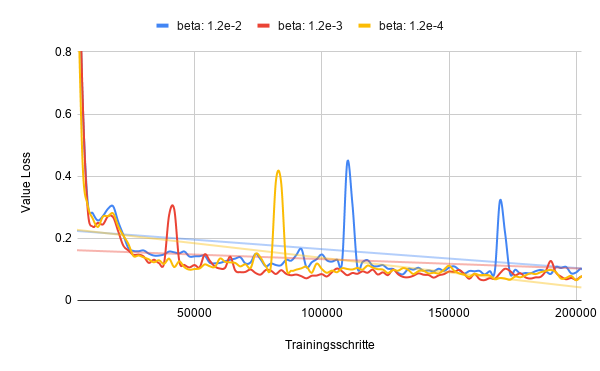
\includegraphics[scale=0.6]{images/training/base_results/result_beta_loss.png}
\caption{Verlauf des Value Loss, Anpassung von \Fachbegriff{beta}}
\label{fig:result_beta_loss}
\end{figure}

\begin{figure}[H]
\centering
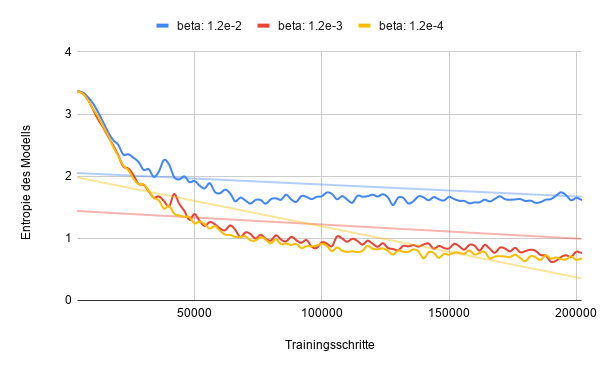
\includegraphics[scale=0.6]{images/training/base_results/result_beta_entropy.png}
\caption{Entropieverlauf, Anpassung von \Fachbegriff{beta}}
\label{fig:result_beta_entropy}
\end{figure}


Insgesamt konnten mit niedrigeren Werten für $\beta$ schneller ein besseres Ergebnis erzielt werden. Das gilt für die Belohnungsfunktion, den Value Loss und die Entropie des Modells. Da für den Wert $\beta = 1.2e-3$ jedoch höhere Belohnungen als für den Wert $\beta = 1.2e-4$ erreicht wurden, wird Beta auf den Wert $\beta = 1.2e-3$ festgelegt.



\subsection*{Lambda}
Der Parameter Lambda ($\lambda$) wurde ebenfalls angepasst, wie in den folgenden Grafiken zu erkennen:

\begin{figure}[H]
\centering
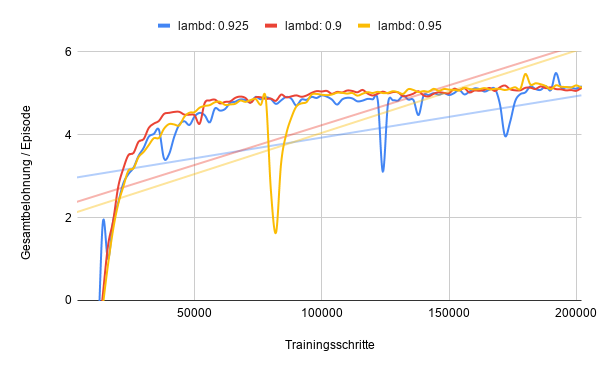
\includegraphics[scale=0.6]{images/training/base_results/result_lambd_rewards.png}
\caption{Belohnungsverlauf, Anpassung von \Fachbegriff{lambd}}
\label{fig:result_lambd_rewards}
\end{figure}

\begin{figure}[H]
\centering
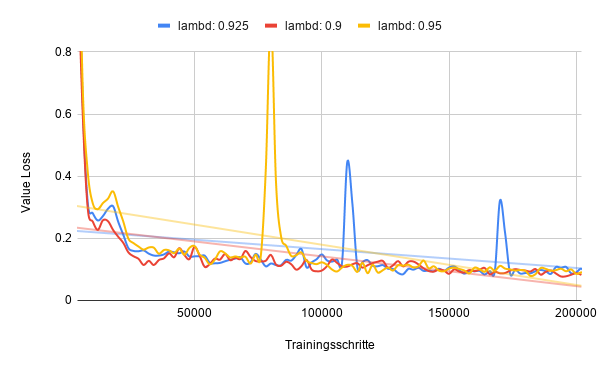
\includegraphics[scale=0.6]{images/training/base_results/result_lambd_loss.png}
\caption{Verlauf des Value Loss, Anpassung von \Fachbegriff{lambd}}
\label{fig:result_lambd_loss}
\end{figure}

\begin{figure}[H]
\centering
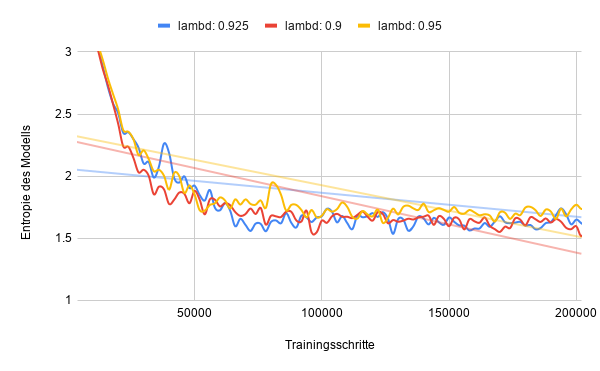
\includegraphics[scale=0.6]{images/training/base_results/result_lambd_entropy.png}
\caption{Entropieverlauf, Anpassung von \Fachbegriff{lambd}}
\label{fig:result_lambd_entropy}
\end{figure}

Die Belohnungsfunktion stabilisiert sich leicht durch die Verwendung eine niedrigeren Wertes für $\lambda$. Auch für die Value Loss- und Entropiefunktion ergibt sich ein leicht verbessertes Ergebnis. Der niedrigste Wert $\lambda = 0.9$ führt also insgesamt zum besten Ergebnis.



\subsection*{Anzahl der Epochen}
Ein weiterer Trainingsdurchlauf wird mit einer reduzierten Anzahl \Fachbegriff{num\_epoch} von vier auf drei Epochen durchgeführt. Dadurch wird derselbe Buffer weniger oft für den Gradientenabstieg verwendet. Geringere Werte sollten in einem stabileren, aber langsameren Training resultieren. ML-Agents empfiehlt einen Minimalwert von $\Fachbegriff{num\_epoch} = 3$.

\begin{figure}[H]
\centering
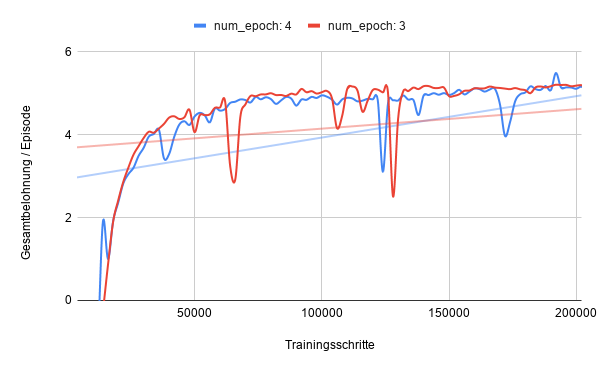
\includegraphics[scale=0.6]{images/training/base_results/result_numepochs_rewards.png}
\caption{Belohnungsverlauf, Anpassung von \Fachbegriff{num\_epochs}}
\label{fig:result_numepochs_rewards}
\end{figure}

\begin{figure}[H]
\centering
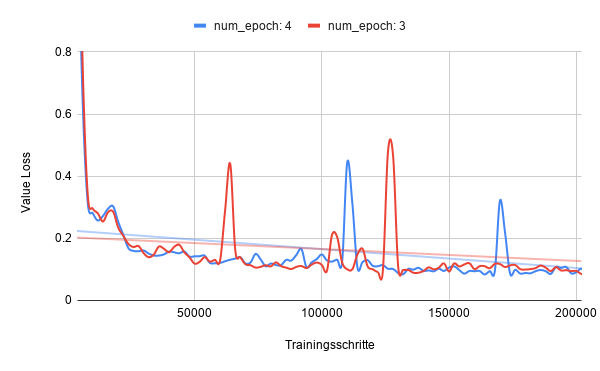
\includegraphics[scale=0.6]{images/training/base_results/result_numepochs_loss.png}
\caption{Verlauf des Value Loss, Anpassung von \Fachbegriff{num\_epochs}}
\label{fig:result_numepochs_loss}
\end{figure}

\begin{figure}[H]
\centering
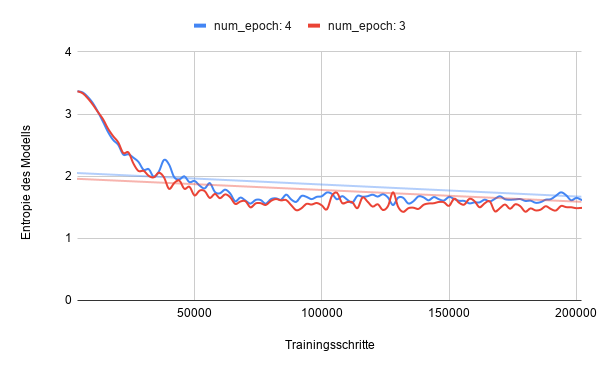
\includegraphics[scale=0.6]{images/training/base_results/result_numepochs_entropy.png}
\caption{Entropieverlauf, Anpassung von \Fachbegriff{num\_epochs}}
\label{fig:result_numepochs_entropy}
\end{figure}

Da die Belohnungsfunktion schneller ansteigt und insgesamt einen hohen Level erreicht und wegen der leicht verbesserten Entropie, wird der Parameter \Fachbegriff{num\_epoch} auf $3$ festgelegt. 



\subsection*{Epsilon}
Der Hyperparameter \Fachbegriff{epsilon} wird angepasst, um zu bestimmen, wie schnell sich eine Policy im Verlauf des Trainings verändern darf. Die Ergebnisse sind in den folgenden Abbildungen zu erkennen:

\begin{figure}[H]
\centering
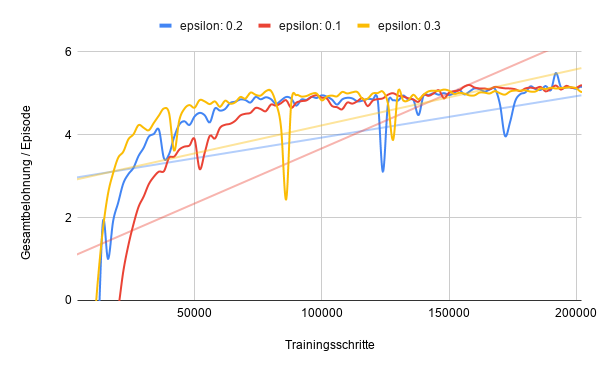
\includegraphics[scale=0.6]{images/training/base_results/result_epsilon_rewards.png}
\caption{Belohnungsverlauf, Anpassung von \Fachbegriff{epsilon}}
\label{fig:result_epsilon_rewards}
\end{figure}

\begin{figure}[H]
\centering
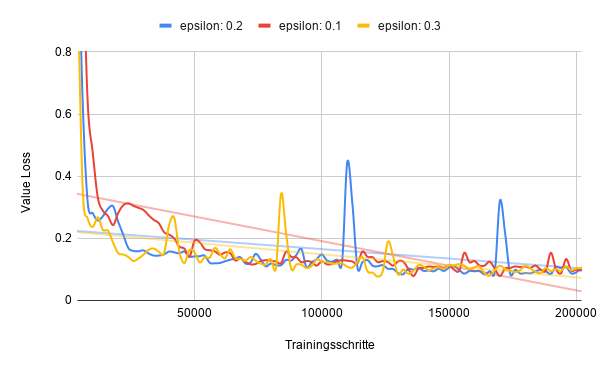
\includegraphics[scale=0.6]{images/training/base_results/result_epsilon_loss.png}
\caption{Verlauf des Value Loss, Anpassung von \Fachbegriff{epsilon}}
\label{fig:result_epsilon_loss}
\end{figure}

\begin{figure}[H]
\centering
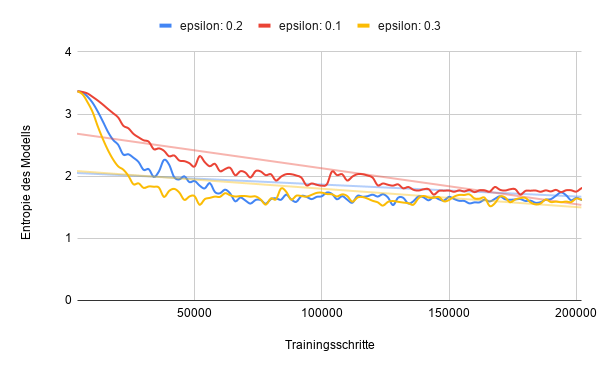
\includegraphics[scale=0.6]{images/training/base_results/result_epsilon_entropy.png}
\caption{Entropieverlauf, Anpassung von \Fachbegriff{epsilon}}
\label{fig:result_epsilon_entropy}
\end{figure}

Wenn der Wert $0.3$ für den Parameter \Fachbegriff{epsilon} gewählt wird, erfolgen daraus insgesamt leicht verbesserte Ergebnisse für alle drei Metriken. Weiterhin wird die Geschwindigkeit des Lernvorgangs erhöht. Dieser Wert wird daher für das finale Training verwendet.




\subsection*{Größe des Buffers}
Weiterhin wird die Größe des Buffers angepasst, um die Auswirkungen dieser Änderungen im Training zu betrachten.

\begin{figure}[H]
\centering
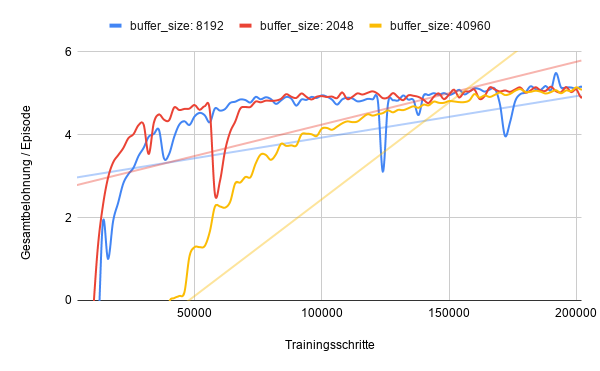
\includegraphics[scale=0.6]{images/training/base_results/result_buffer_rewards.png}
\caption{Belohnungsverlauf, Anpassung von \Fachbegriff{buffer\_size}}
\label{fig:result_buffer_rewards}
\end{figure}

\begin{figure}[H]
\centering
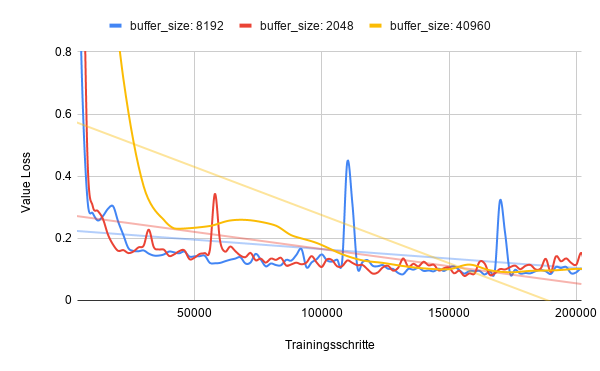
\includegraphics[scale=0.6]{images/training/base_results/result_buffer_loss.png}
\caption{Verlauf des Value Loss, Anpassung von \Fachbegriff{buffer\_size}}
\label{fig:result_buffer_loss}
\end{figure}

\begin{figure}[H]
\centering
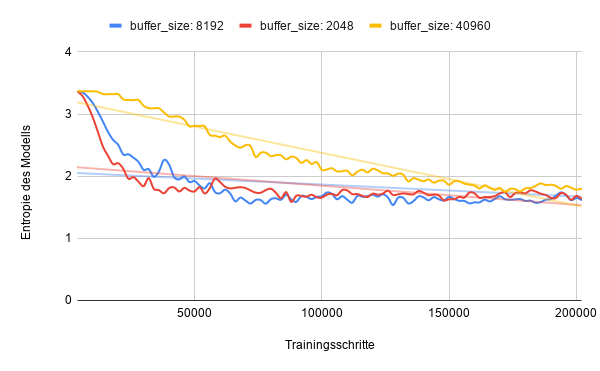
\includegraphics[scale=0.6]{images/training/base_results/result_buffer_entropy.png}
\caption{Entropieverlauf, Anpassung von \Fachbegriff{buffer\_size}}
\label{fig:result_buffer_entropy}
\end{figure}

Die höchste Buffergröße führt zu einem deutlich verlangsamten Trainingsvorgang mit insgesamt schlechteren Ergebnissen für Belohnungen, Value Loss und die Entropie.
Für niedrige Werte erfolgt ein leicht schnellerer Lernvorgang mit ähnlichen Endergebnissen für die Belohnungswerte. Da sich die Entropie und der Value Loss jedoch nicht verändern, wird weiterhin der Wert $8192$ für die Buffergröße gewählt.


%\chapter*{Literaturverzeichnis}
\bibliography{listings/thesis} % create with BibTeX

\newpage
\include{base/footer}

\end{document}
